\chapter{Proposed Non-local Modeling Method}
\graphicspath{{Chapter4/}}
\label{chap:chapter4}

\section{Motivation}
The HVS perceives image quality by capturing local distortions and aggregating non-local dependencies~\citep{golestaneh2021no, liu2020long}. In particular, the strong dependencies among neighborhood pixels carry essential information of the structure of objects, which is sensitively perceptive by HVS for quality evaluation~\citep{wang2004image}. On the other hand, the non-local features have also been revealed to play a complementary role in human quality rating~\citep{zontak2011internal}.

Following this vein, for the exploration of local quality clues, a pre-trained VGGNet~\citep{SimonyanZ14a} is adopted, whose effectiveness has been validated in acquiring highly quality-aware features and is widely used for both FR-IQA tasks~\citep{ding2021comparison} and NR-IQA tasks~\citep{liu2017rankiqa}. Nevertheless, there is a strong inductive bias in CNN,~\ie, locality. Suffered by the local priors to CNN, the non-local information is usually absent. To account for this, we further design a superpixel-based GNN approach to capture the non-local features. Finally, the local and non-local features are fused for image quality regression. Experimental results have demonstrated the complementary role of the local and non-local features, and superior performance can be achieved by combining the two types of features.

\section{Contribution}
\begin{itemize}
	\item We propose a novel NR-IQA framework based on the GNN. The non-local behavior of natural images is emphasized and learned in our proposed \textbf{N}on-\textbf{L}ocal dependency \textbf{Net}work (termed as NLNet).
	\item The spatial attention module is introduced to integrate the information of long- and short-range communications among graph nodes of the entire image.
	\item Extensive experimental results reveal that the proposed NLNet manages to extract the non-local information for quality prediction, and the superior performance in cross-dataset settings verifies the high generalization capability of our proposed method.
\end{itemize}

\section{The Proposed Scheme}
\begin{figure*}[ht]
	\centering
	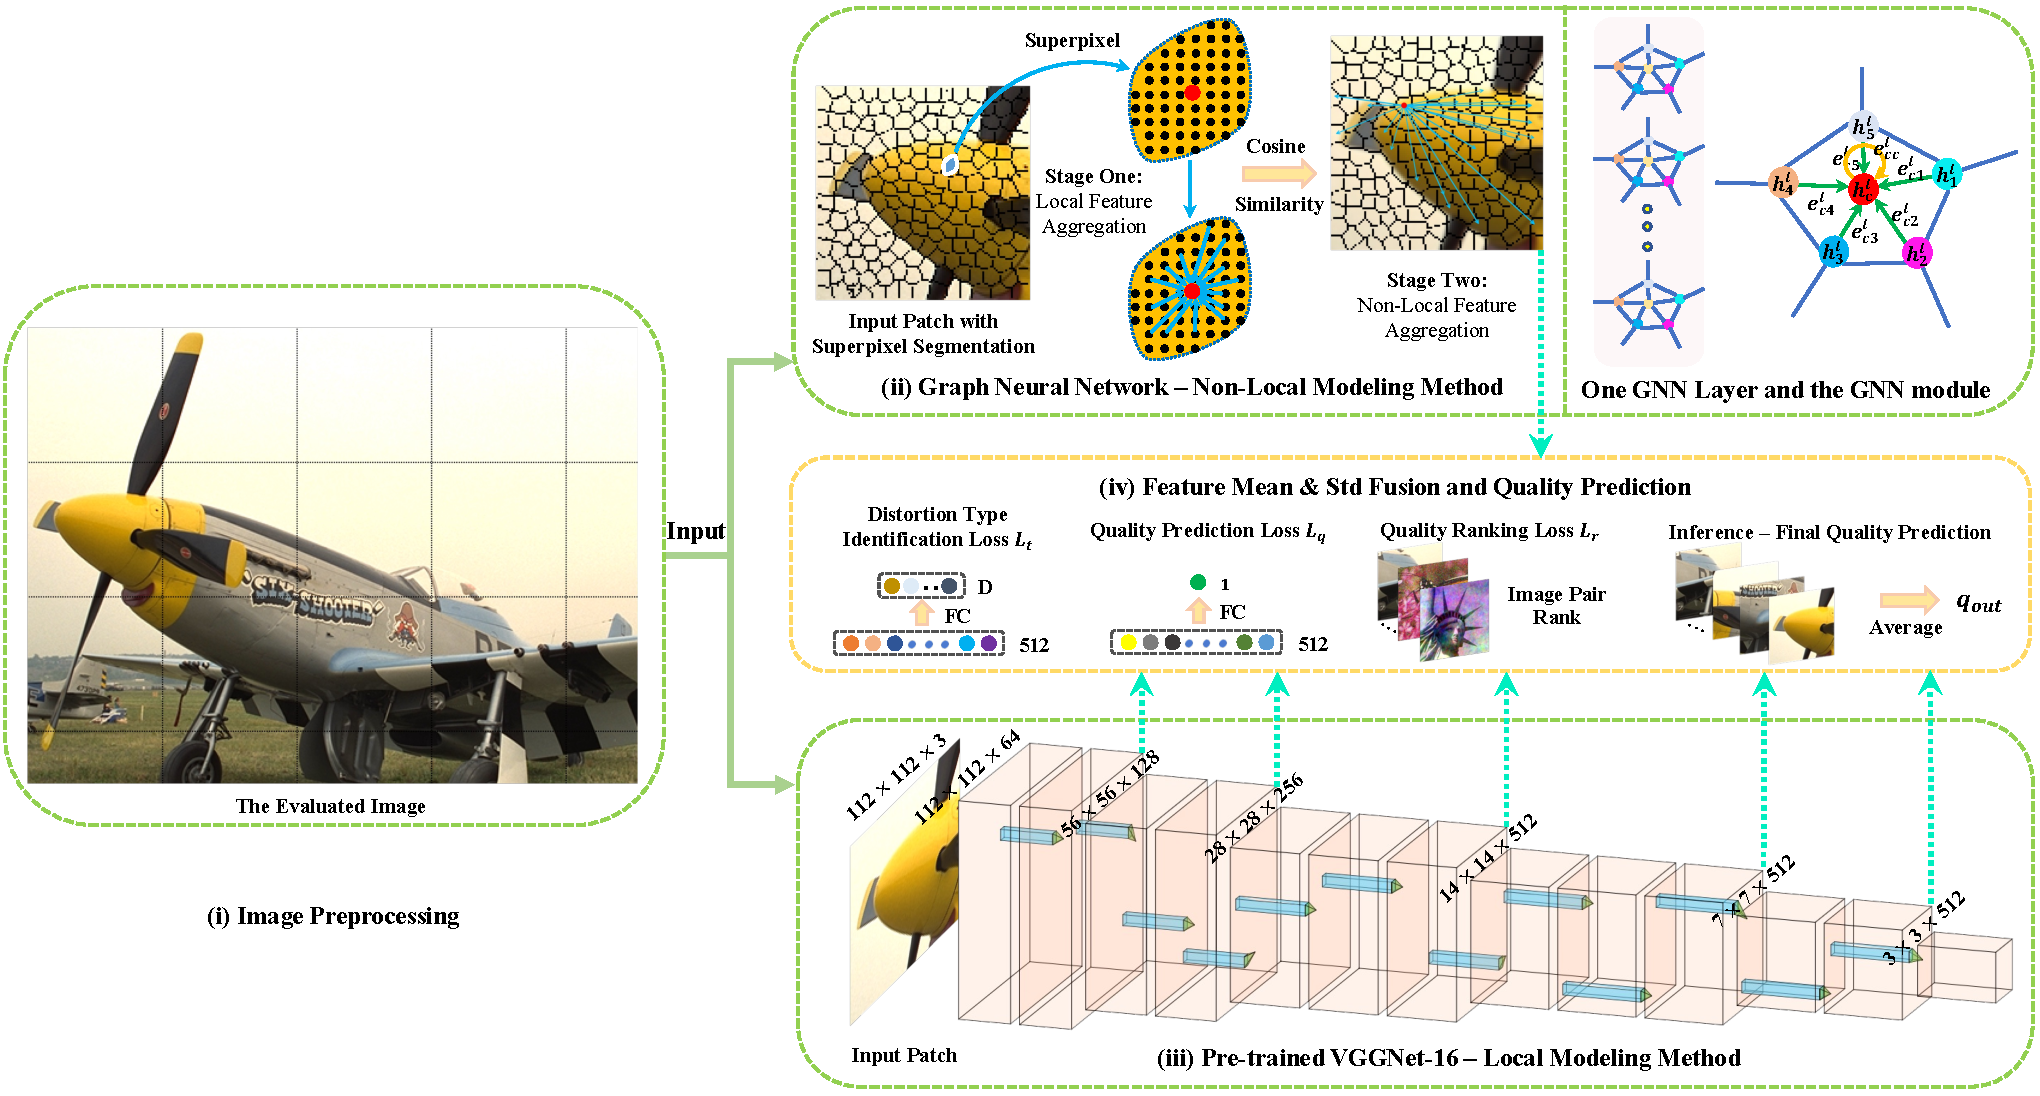
\includegraphics[width=\linewidth]{fig/overview.pdf}
	\caption{An overview of the proposed NLNet.}
	\label{Overview}
\end{figure*}

In~\reffig{Overview}, we present the proposed non-local modeling method. The details are described as follows:
\begin{enumerate}[label=\roman*.]
	\item The input image is pre-processed.
	\item A two-stage GNN approach is presented for the non-local feature extraction and long-range dependency construction among different regions. The first stage aggregates local features inside superpixels. The following stage learns the non-local features and long-range dependencies among graph nodes. It then integrates short- and long-range information based on an attention mechanism. The means and standard deviations of the non-local features are obtained from the graph feature signals.
	\item Local feature means and standard deviations are derived from the pre-trained VGGNet-16 considering the hierarchical degradation process of the HVS.
	\item The means and standard deviations of the local and non-local features are fused to deliver a robust and comprehensive representation for quality assessment. Besides, the distortion type identification loss $L_t$, quality prediction loss $L_q$, and quality ranking loss $L_r$ are utilized for training the NLNet. During inference, the final quality of the image is the averaged quality of all the non-overlapping patches.
\end{enumerate}

This work presents a hybrid of local and non-local feature extractions to assess image quality. We propose a superpixel-based GNN to learn the non-local features and capture long-range dependencies. Meanwhile, a pre-trained VGGNet-16 is employed to extract local features from spatially proximate neighborhoods. Finally, the non-local features from GNN and local features from CNN are fused to predict the quality. In the following paragraphs, we first introduce the superpixel segmentation. Then, the construction of GNN is provided, and finally, the local and non-local feature fusion is elaborated~\footnote{~Source codes of the proposed method are publicly accessible at https://github.com/SuperBruceJia/NLNet-IQA for scientific reproducible research.}.

	\subsection{Superpixel Segmentation and Divisive Normalization}
	\begin{figure*}[!ht]
		\centering
		\begin{minipage}[t]{.49\linewidth}
			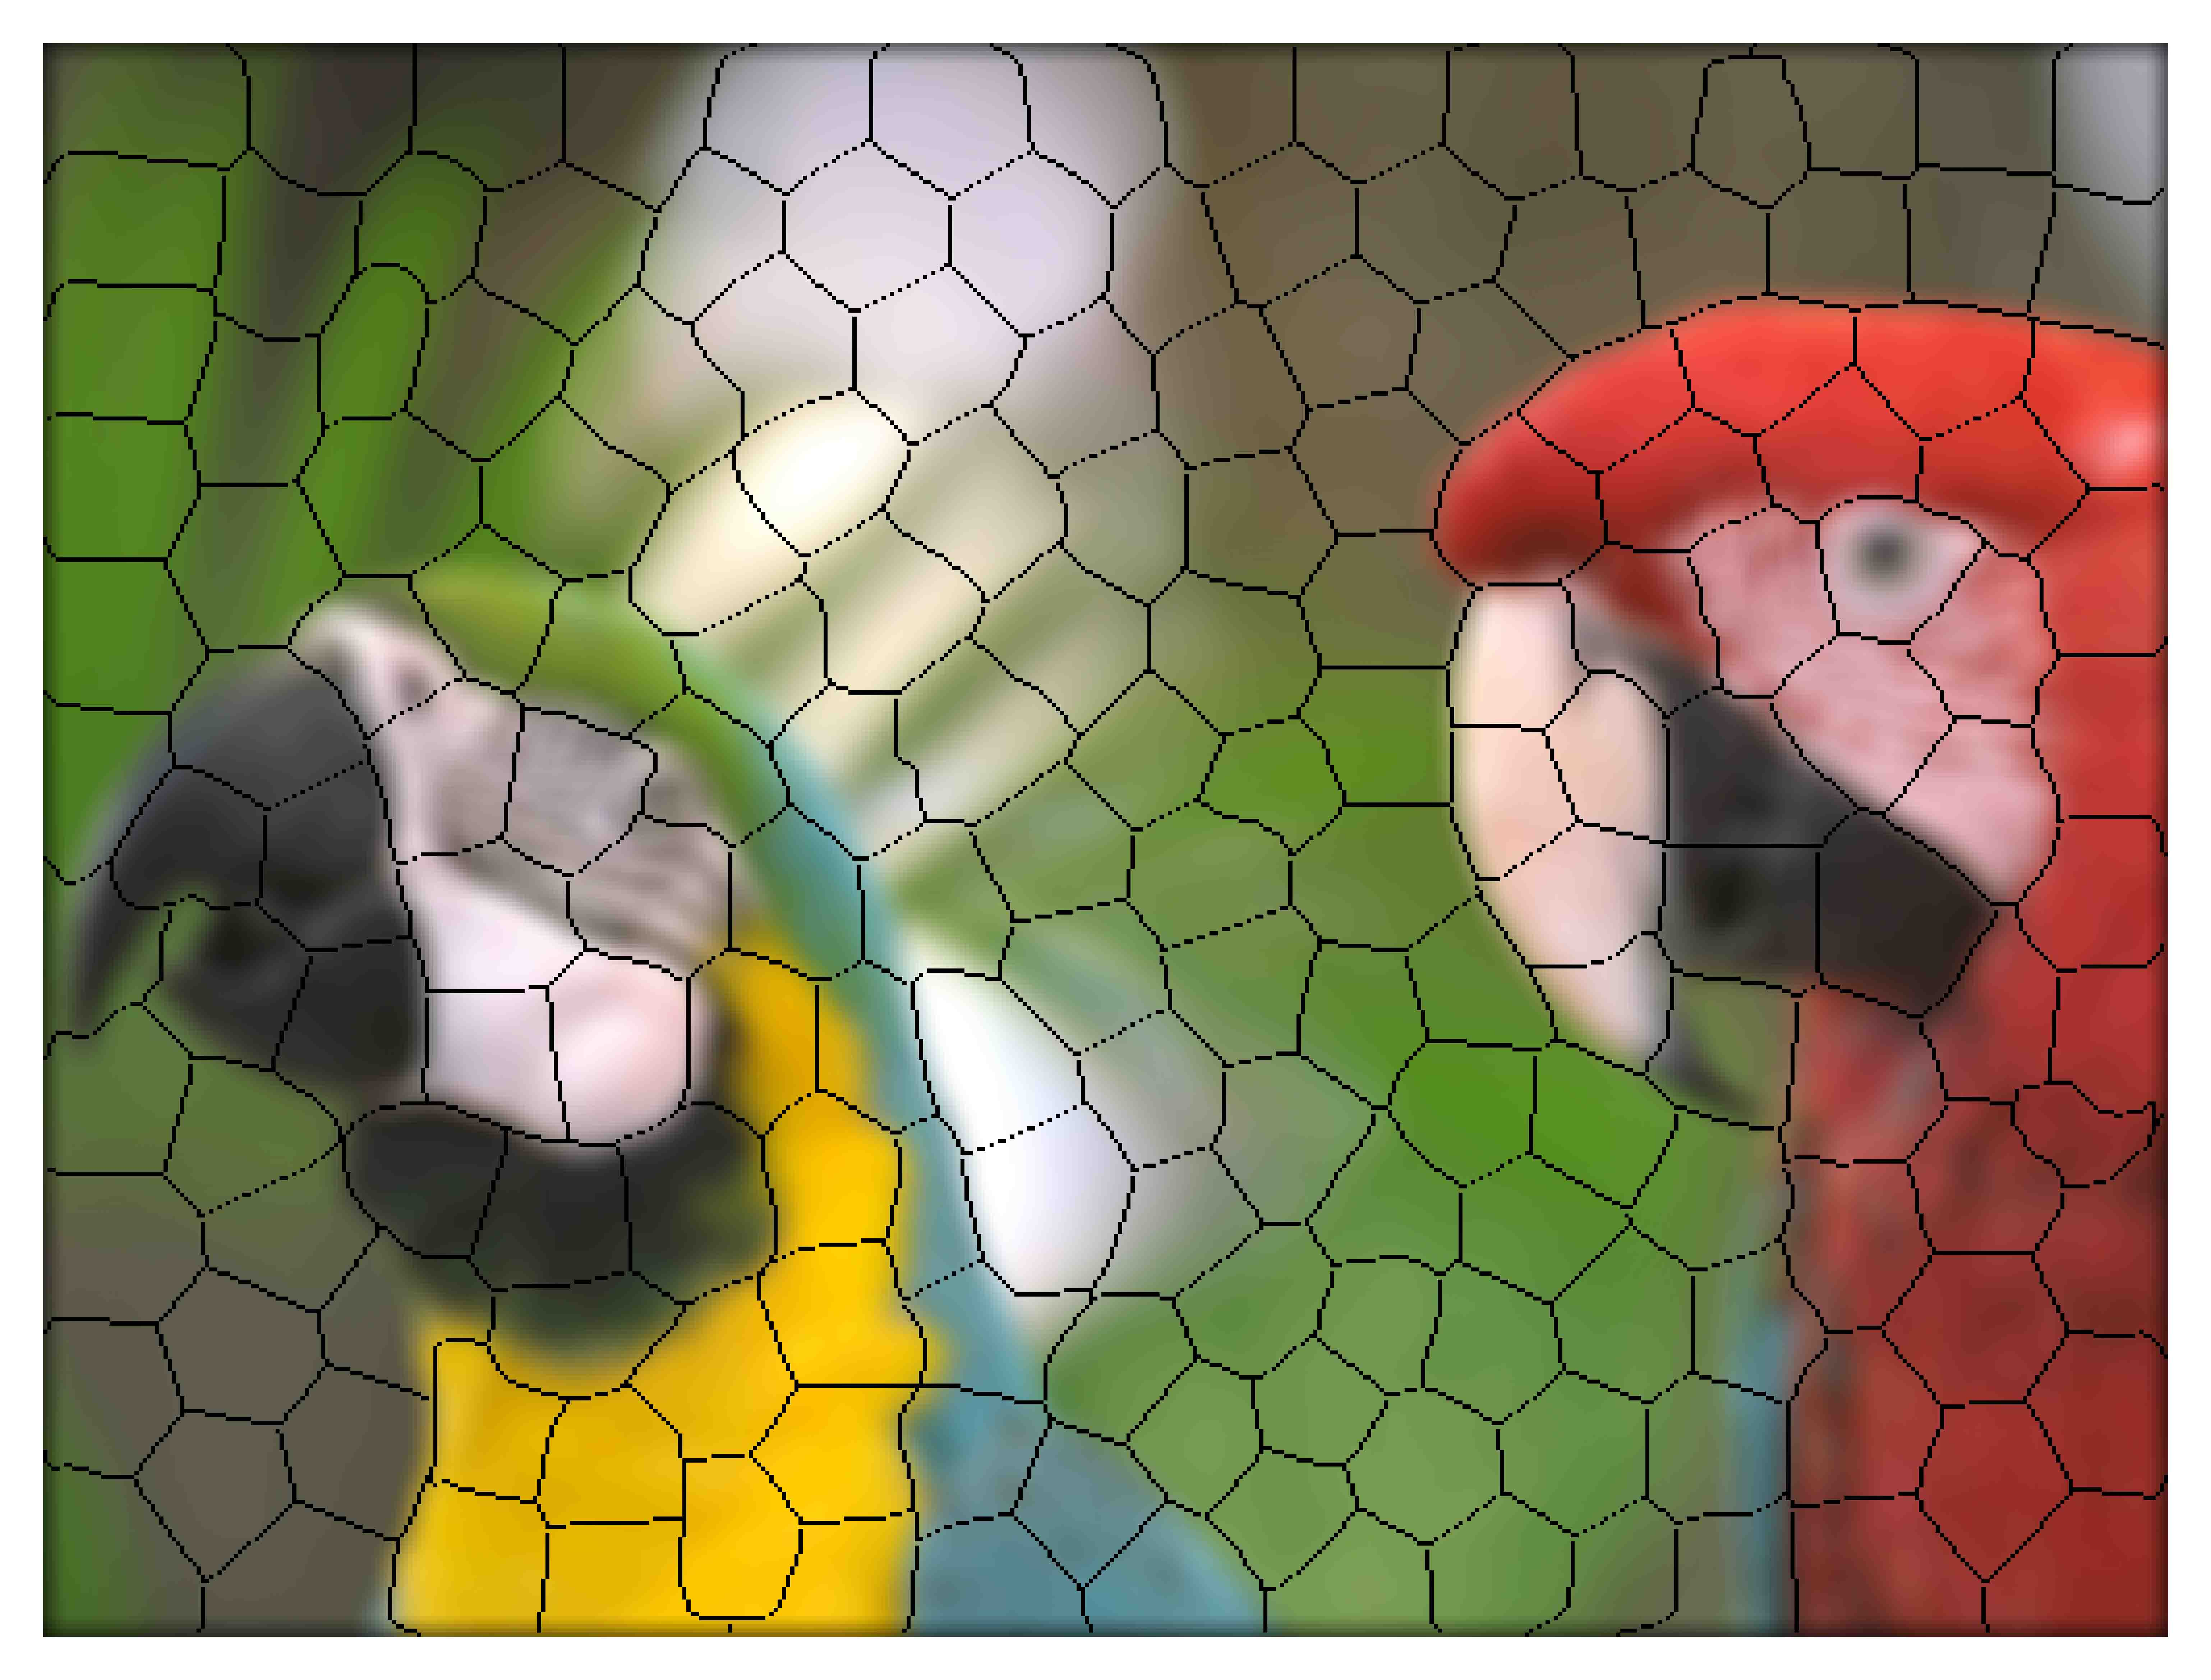
\includegraphics[width=2.8in]{fig/parrot_superpixel_gaussian_blur.jpg}
			\centerline{(a)}
			\label{PARROT-superpixel-Gaussian-Blur}
		\end{minipage}
		\begin{minipage}[t]{.49\linewidth}
			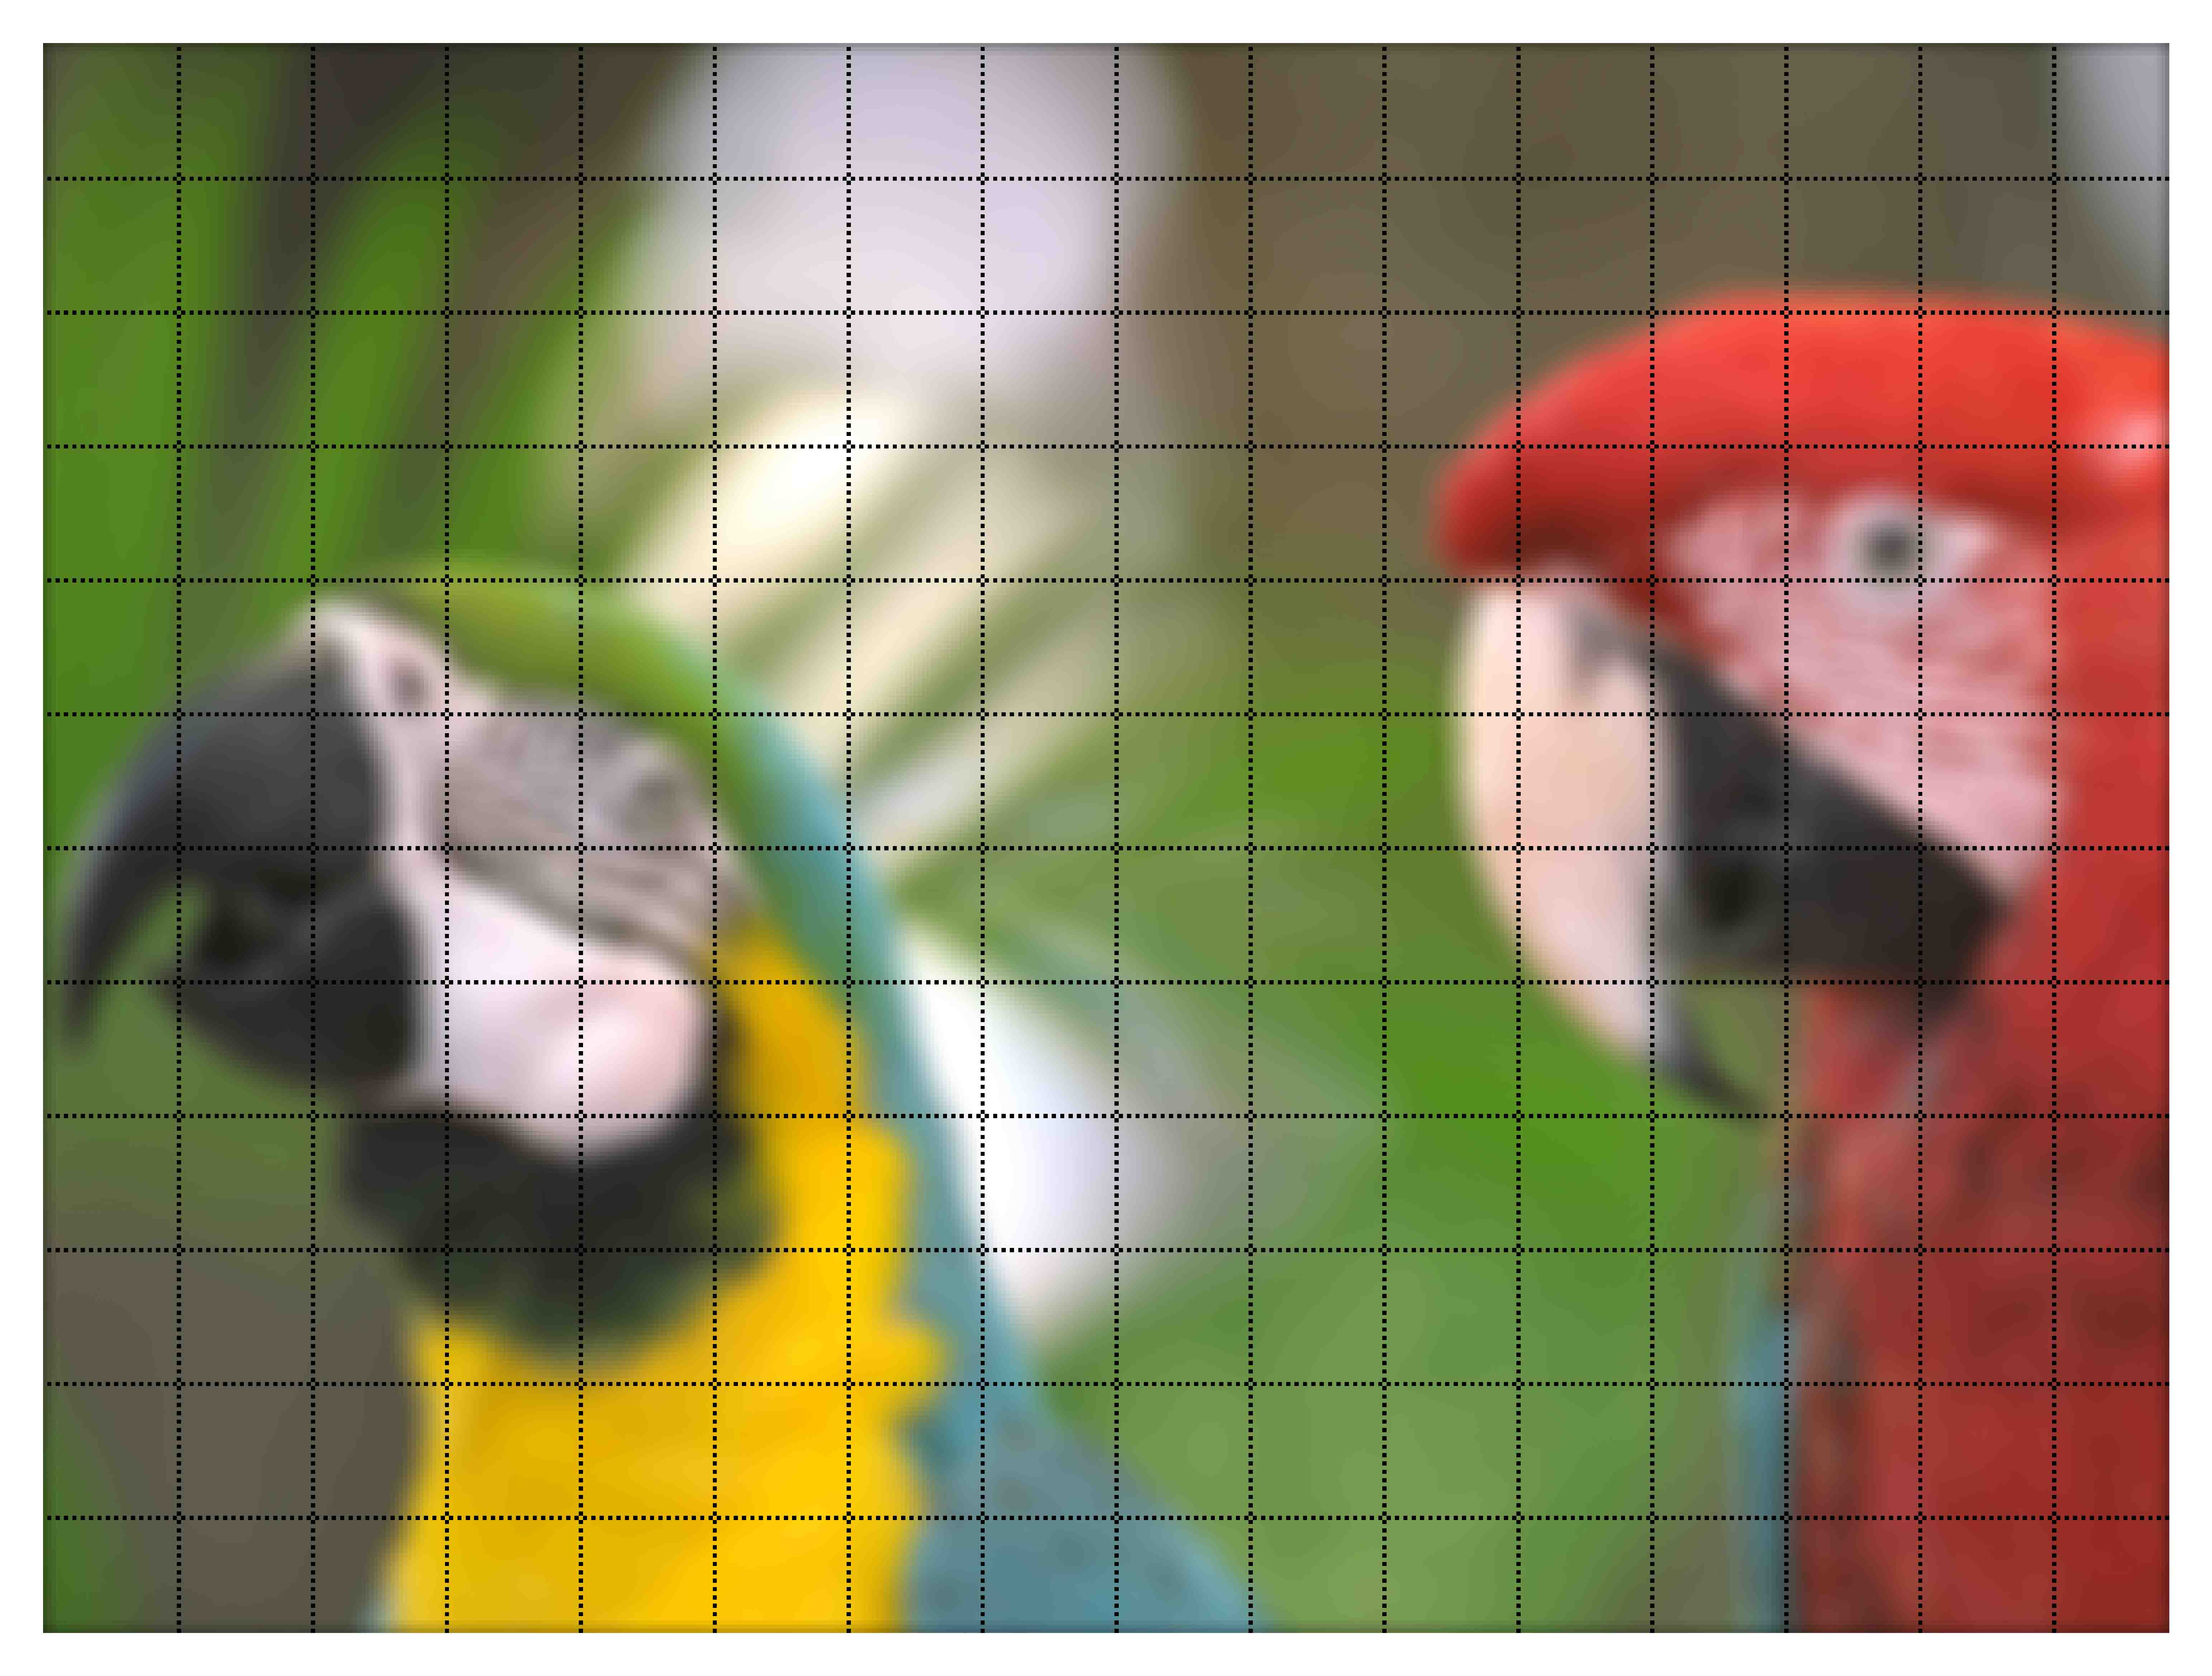
\includegraphics[width=2.8in]{fig/parrot_square_gaussian_blur.jpg}
			\centerline{(b)}
			\label{PARROT-square-grid-Gaussian-Blur}
		\end{minipage}
		\begin{minipage}[t]{.49\linewidth}
			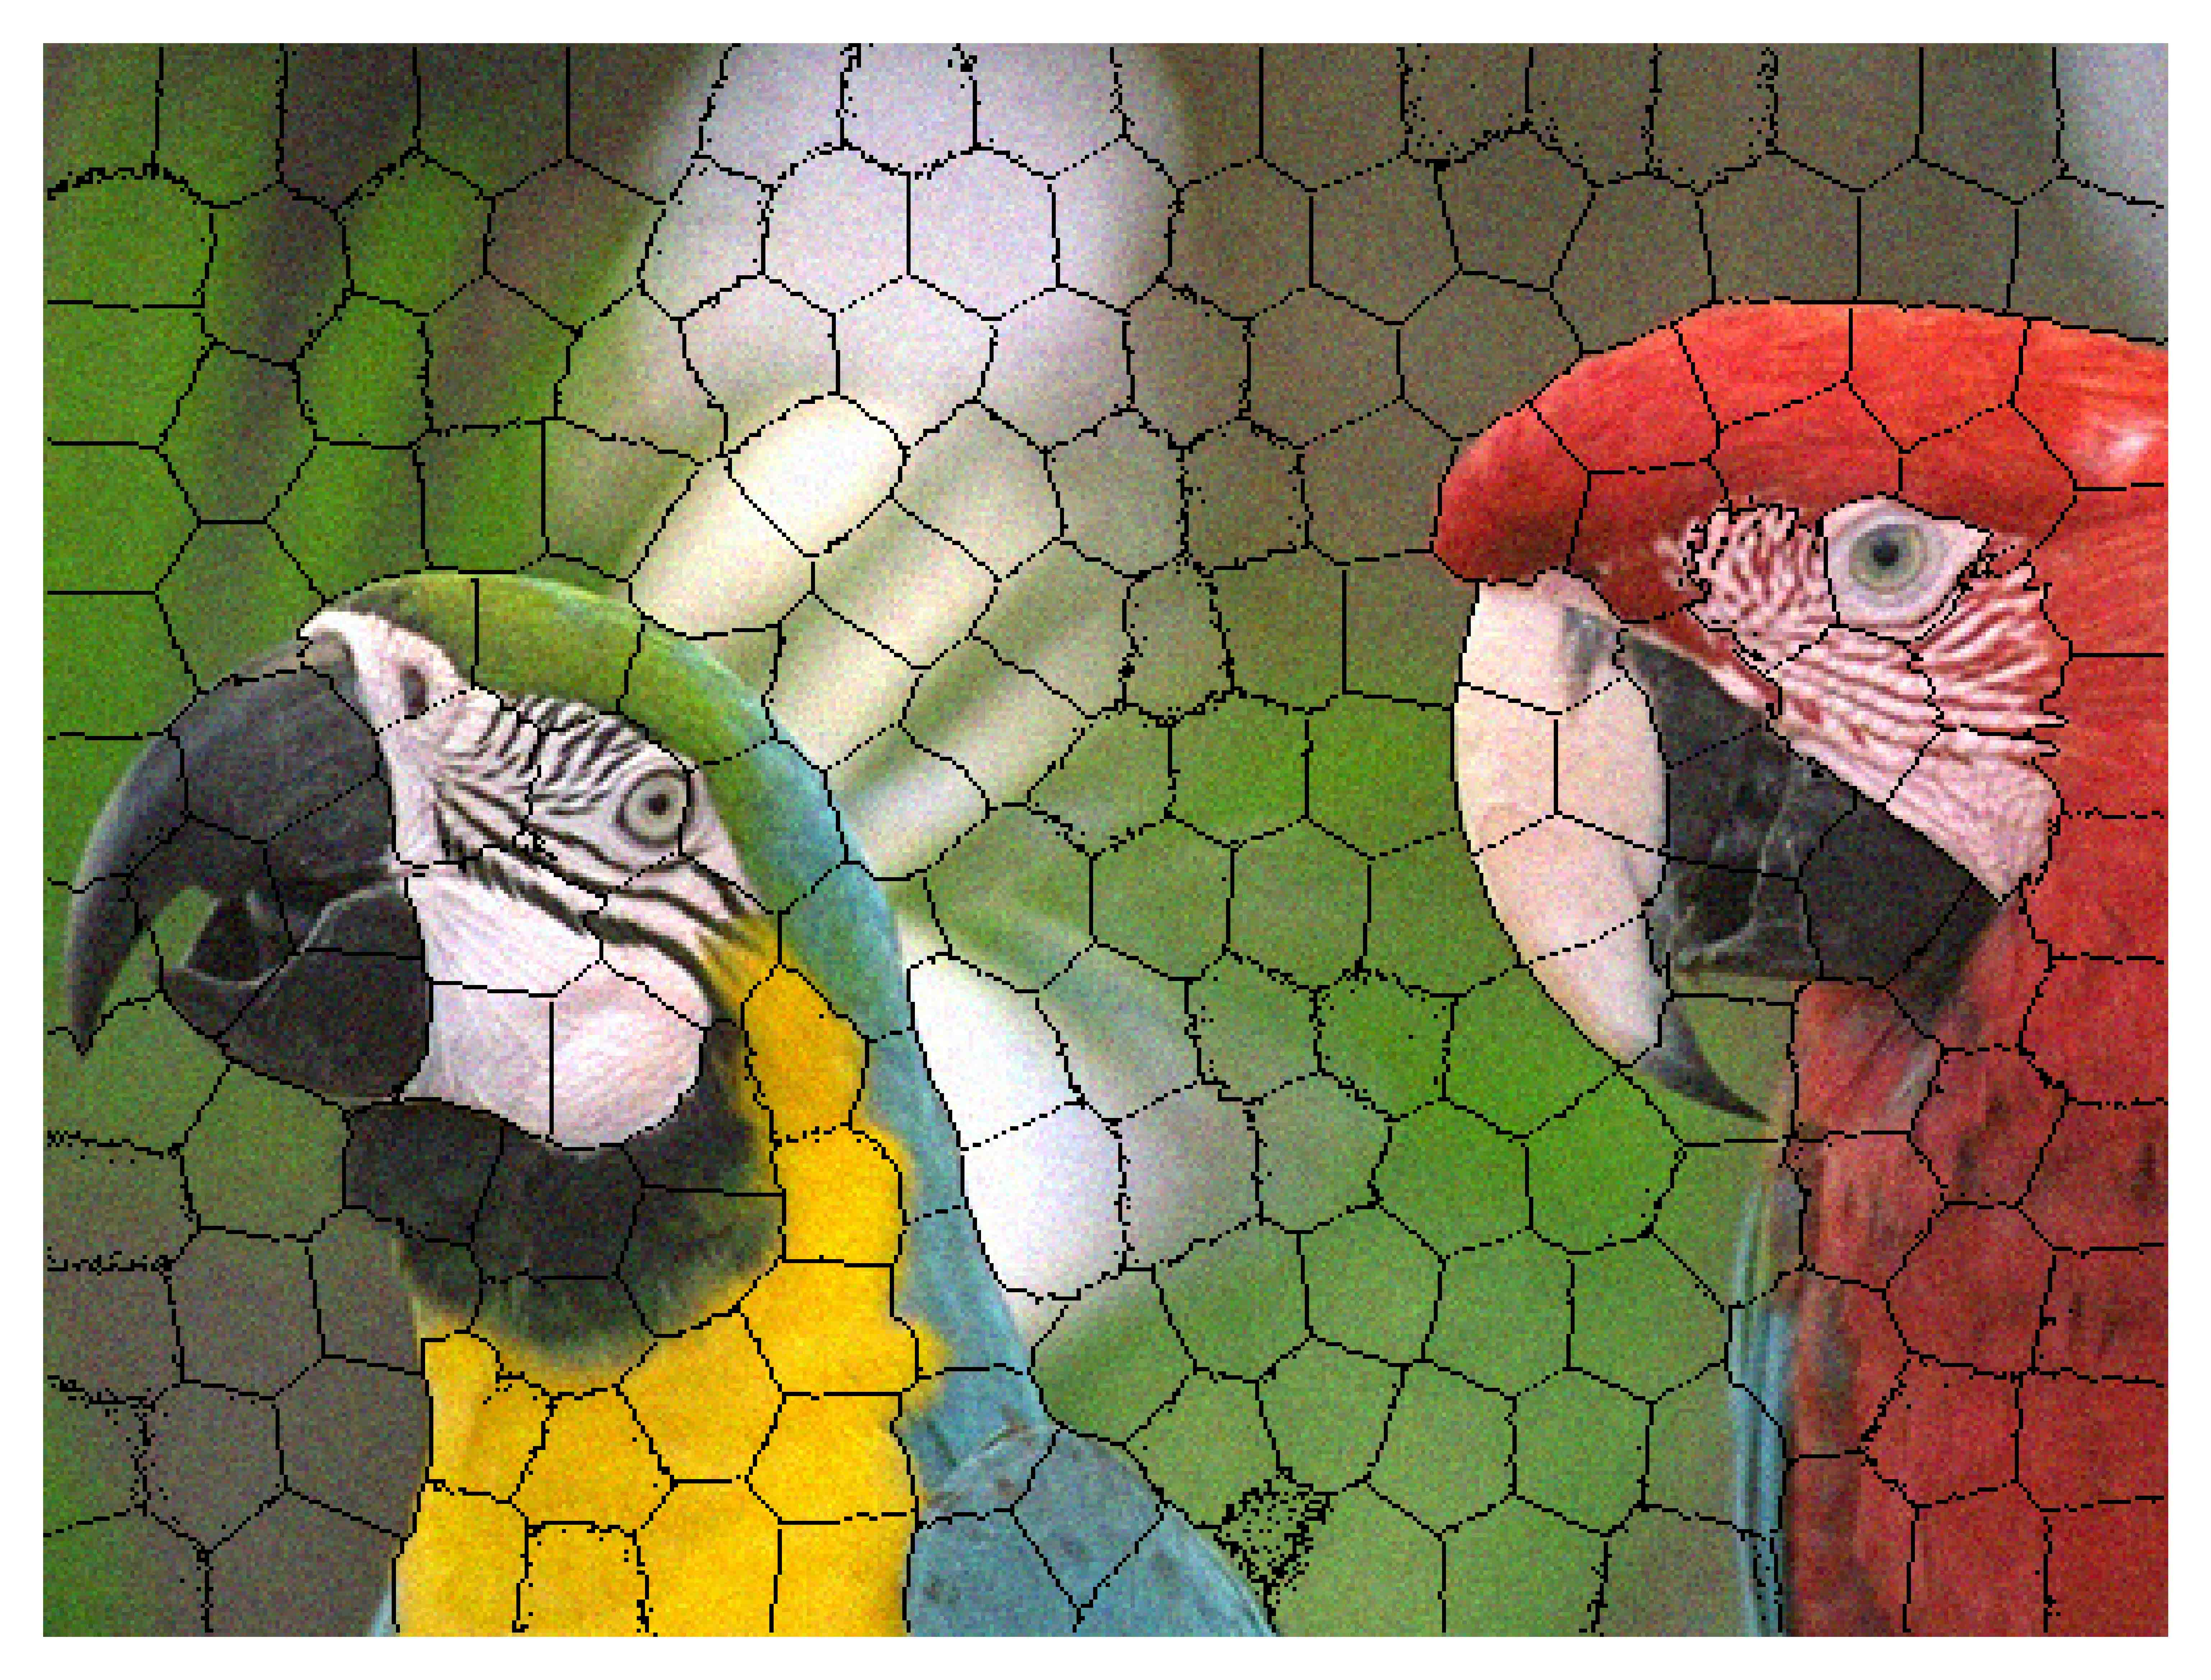
\includegraphics[width=2.8in]{fig/parrot_superpixel_gaussian_noise.jpg}
			\centerline{(c)}
			\label{PARROT-superpixel-Gaussian-Noise}
		\end{minipage}
		\begin{minipage}[t]{.49\linewidth}
			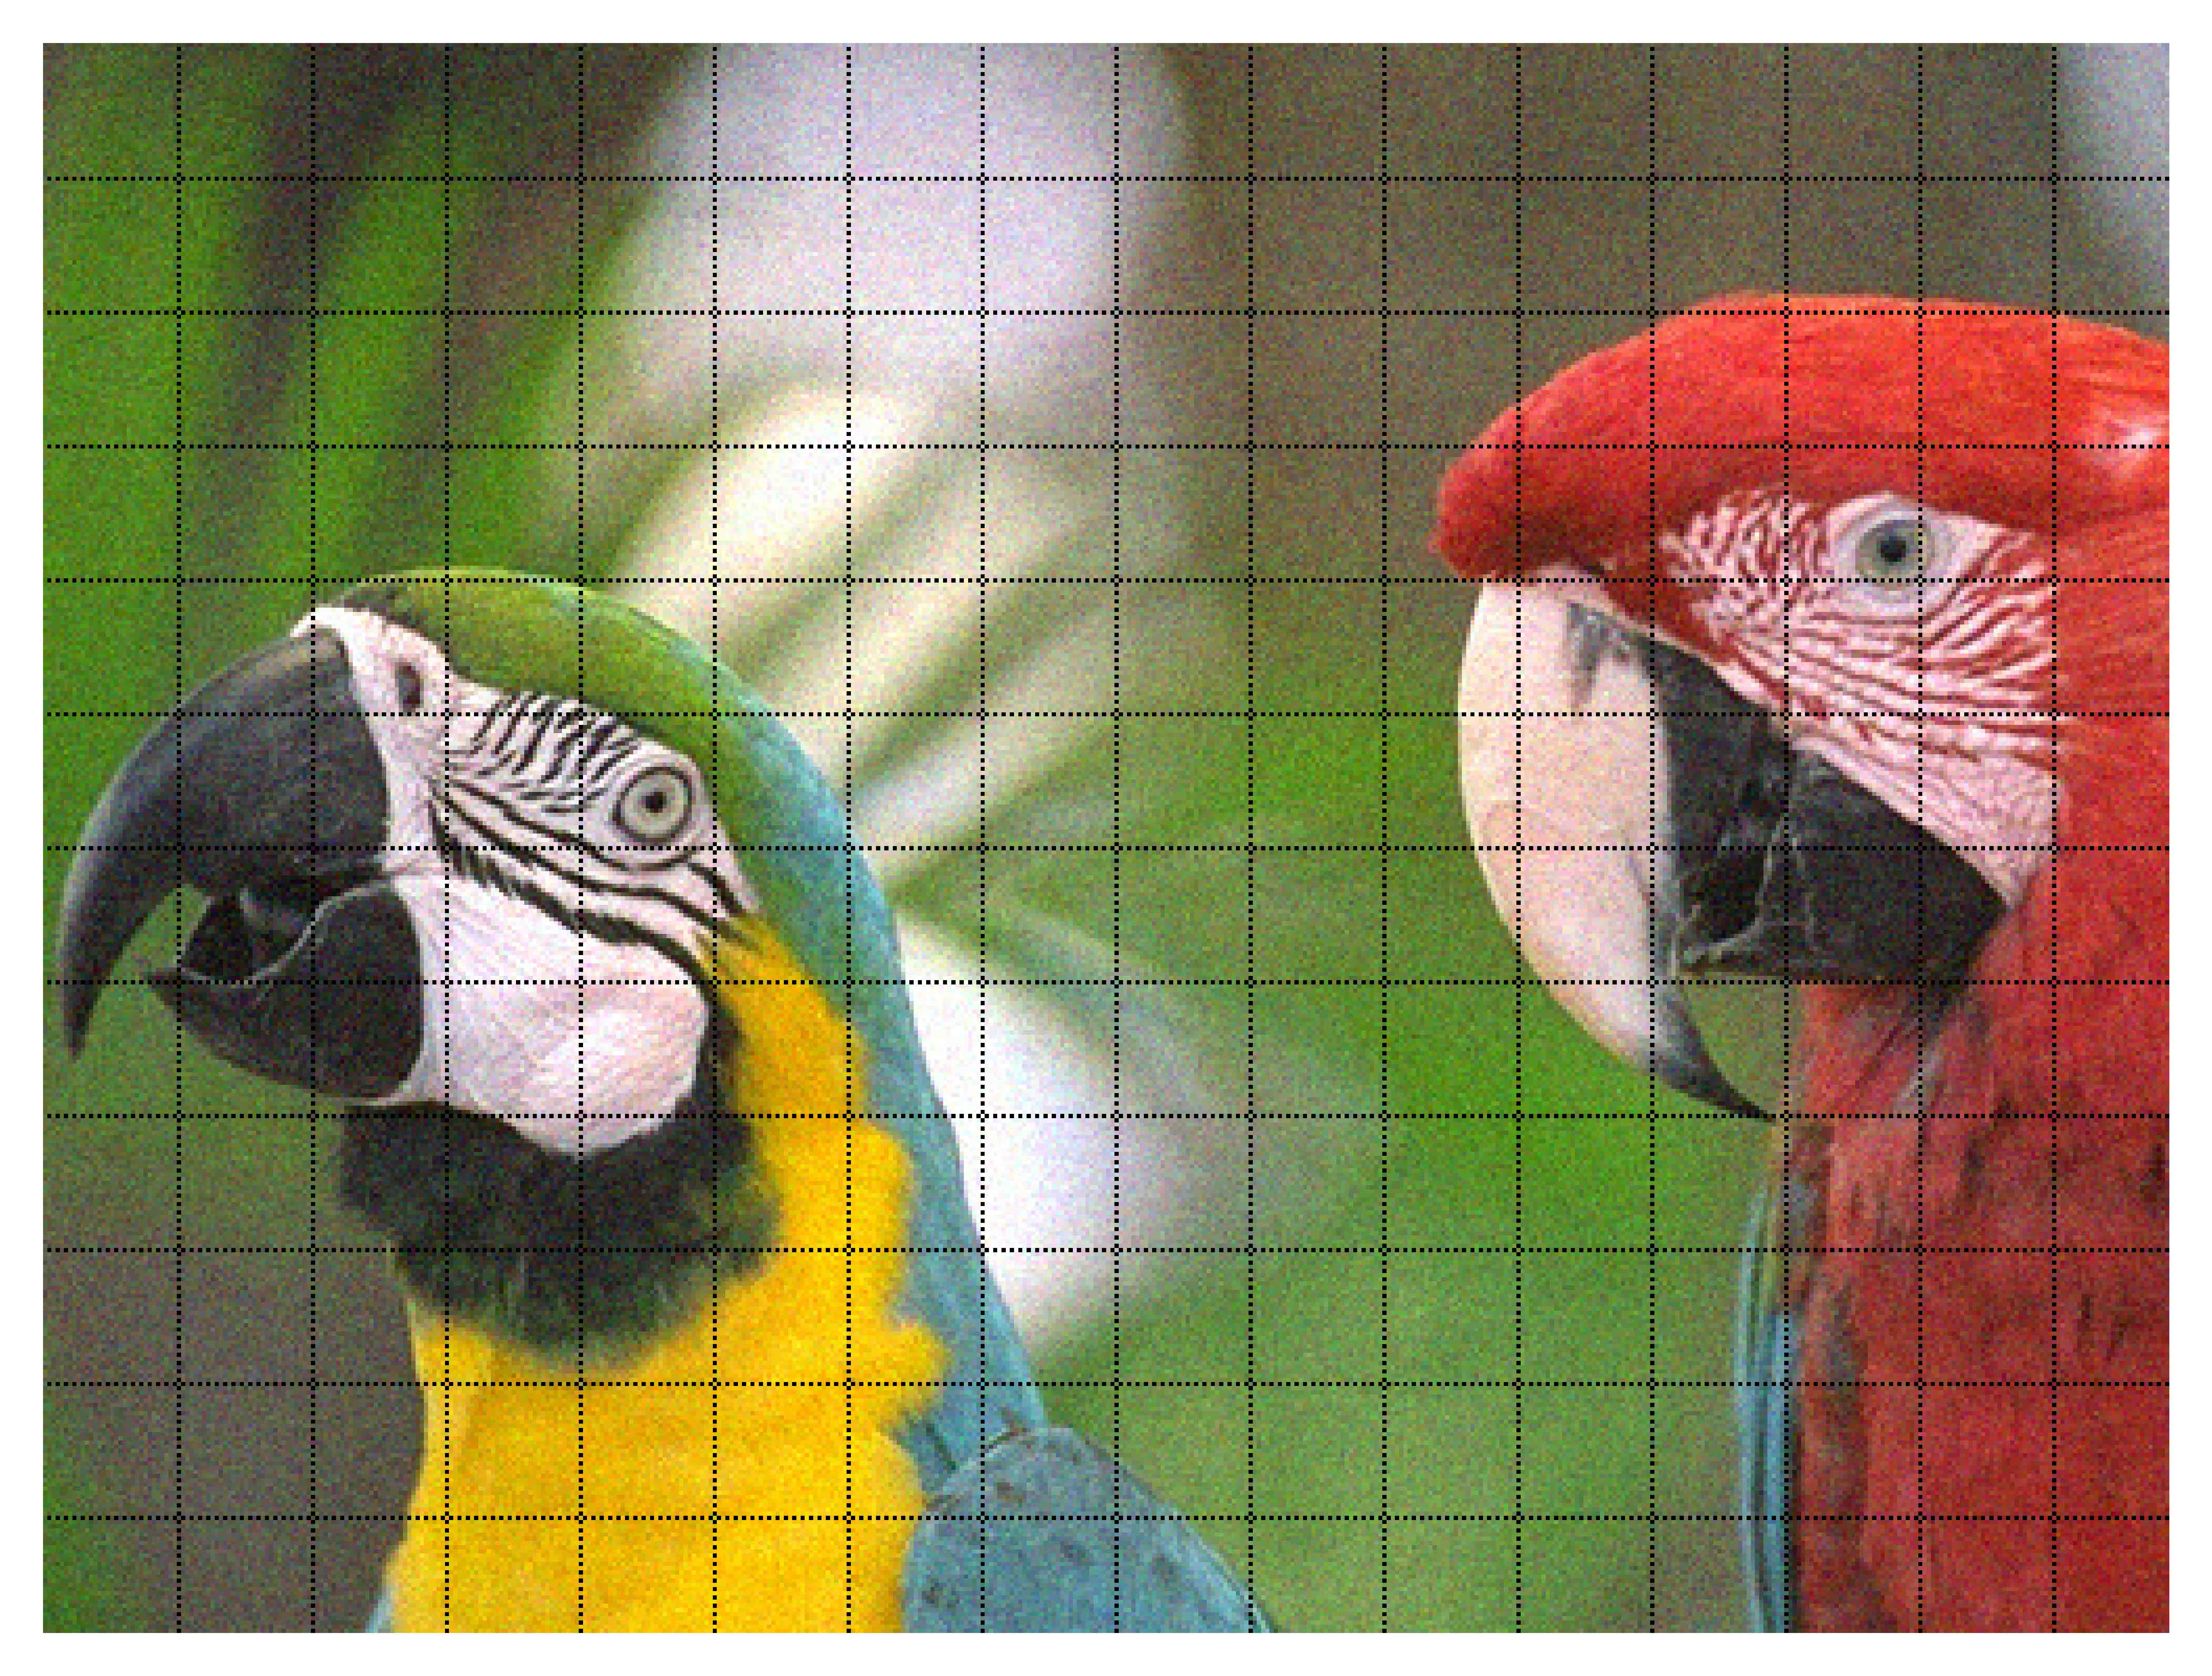
\includegraphics[width=2.8in]{fig/parrot_square_gaussian_noise.jpg}
			\centerline{(d)}
			\label{PARROT-square-grid-Gaussian-Noise}
		\end{minipage}
		\caption{The superpixel~\emph{vs.} square patch representation (with size of $\approx 32 \times 32$) of the parrot image from the TID2013 database.}
		\label{The superpixel versus square patch of the parrot image from the TID2013 database}
	\end{figure*}
	A superpixel is a group of pixels with similar visual characteristics, such as color, intensity, and spatial adjacency. The superpixel segmentation methods are broadly performed in the pre-processing stage for CV tasks, such as reducing dimensionality, alleviating the computational load, and removing outliers and irrelevant details~\citep{achanta2012slic}. Superpixels can be represented as graphs and processed via graph representation learning methods,~\eg, GNN~\citep{Giraldo2022Graph}. Compared with features derived from the standard pixel grids, superpixels can be adaptive to the regional content and generate more meaningful representations. Thus, the NSS can be well-exploited, which has been validated for FR-IQA~\citep{sun2018spsim, 9198131}. 
	
	We demonstrate superpixel segmentations in~\reffig{The superpixel versus square patch of the parrot image from the TID2013 database}.~\reffig{The superpixel versus square patch of the parrot image from the TID2013 database}~(a) to~\reffig{The superpixel versus square patch of the parrot image from the TID2013 database}~(d) are described as follows:~\reffig{The superpixel versus square patch of the parrot image from the TID2013 database}~(a) The superpixel segmentation of the parrot image distorted by the Gaussian blur.~\reffig{The superpixel versus square patch of the parrot image from the TID2013 database}~(b) The square patch representation of the parrot image distorted by the Gaussian blur.~\reffig{The superpixel versus square patch of the parrot image from the TID2013 database}~(c) The superpixel segmentation of the parrot image distorted by the white Gaussian noise.~\reffig{The superpixel versus square patch of the parrot image from the TID2013 database}~(d) The square patch representation of the parrot image distorted by the white Gaussian noise. Two advantages of applying superpixels are summarized as follows.
		
		\subsubsection{Adhere to Boundaries and Visually Meaningful}\label{Adhere to Boundaries and Visually Meaningful}
		As can be seen from~\reffig{The superpixel versus square patch of the parrot image from the TID2013 database}~(a), the aggregated pixels compose a visually and perceptually meaningful atomic region by sharing related features. They exhibit different structures and textures and reflect local image characteristics. Besides, HVS is adaptive to local content, which is multi-scale and spatially non-stationary. Image information inside regular square patches (see~\reffig{The superpixel versus square patch of the parrot image from the TID2013 database}~(b) and~\reffig{The superpixel versus square patch of the parrot image from the TID2013 database}~(d)) may not be precise and adequate to represent the multi-scale and dynamic visual contexts~\citep{sun2018spsim}. In contrast, superpixels adhere to image boundaries. Thus, they are adaptive to regional content and perceptually more meaningful.
		
		\subsubsection{Accurate Feature Extraction}\label{Accurate Feature Extraction}
		Extracting low-level features from superpixels is more accurate and reliable than square patches. Evidence for this is in~\reffig{The superpixel versus square patch of the parrot image from the TID2013 database}~(a) and~\reffig{The superpixel versus square patch of the parrot image from the TID2013 database}~(c), where pixels inside a superpixel share similar characteristics, such as texture and flat regions. Features inside superpixels describe the image in detail and preserve the topological properties of the image. A local square patch may contain regions of texture and flat, especially near their boundaries. The texture areas are sensitive to the Gaussian blur but robust to Gaussian noise, while the flat regions are opposite (\reffig{The superpixel versus square patch of the parrot image from the TID2013 database}~(a) and~\reffig{The superpixel versus square patch of the parrot image from the TID2013 database}~(c)). However, a superpixel is mainly a homogeneous area where local variations and structures are distributed within the boundary. Features, especially the low-level statistics obtained from superpixels, are much more accurate. Therefore, it is of great benefit to analyze the properties of local regions via superpixels.
	
	Our method explores the effectiveness of feature extraction from superpixels for NR-IQA. In this work, we adopt the Simple Linear Iterative Clustering (SLIC) algorithm to generate superpixels on account of its efficient computation and exceptional adherence to objects' boundaries~\citep{achanta2012slic, sun2018spsim, 9198131}. First of all, the image is converted and represented in the CIELAB color space~\citep{achanta2012slic}. Then, the SLIC algorithm uniformly allocates cluster centers over the image. Further, based on the K-means clustering~\citep{duda1973pattern}, it assigns each pixel to its nearest center by a pre-defined composite distance in a bounded region. Finally, each cluster center is updated as the mean position of group pixels during iterations. 
	
	Liu~\etal empirically advises to set the size of each superpixel to roughly $\sqrt{N_{ip} / 200}$, where $N_{ip}$ is the number of pixels in the image $\boldsymbol{\mathrm I}$. In this way, superpixels preserve objects' boundaries of a given image~\citep{liu2013superpixel}. The superpixels' value $I^{\prime}(i, j)$ is obtained from the locally normalized image $\boldsymbol{\mathrm{I^{\prime}}}$. We model the contrast-gain and masking process in HVS by removing the local mean $\mu(i, j)$ and dividing the local standard deviation $\sigma(i, j)$~\citep{ma2017end}.
	
	\begin{equation}
		I^{\prime}(i, j) = \frac{I(i, j) - \mu(i, j)}{\sigma(i, j) + C},
		\label{Normalization}
	\end{equation}
	
	\begin{equation}
		\mu(i, j) = \sum_{i^{\prime} j^{\prime}} \omega_{i^{\prime} j^{\prime}} I_{i^{\prime} j^{\prime}}(i, j),
	\end{equation}
	
	\begin{equation}
		\sigma(i, j)=\sqrt{\sum_{i^{\prime} j^{\prime}} \omega_{i^{\prime} j^{\prime}}\left(I_{i^{\prime} j^{\prime}}(i, j)-\mu(i, j)\right)^{2}},
	\end{equation}
	where the weighting matrix $\boldsymbol{\mathrm{\omega}}$ is a two-dimensional circularly-symmetric Gaussian band-pass filter and $C$ is a constant to stabilize training.
	
	\begin{equation}
		\boldsymbol{\mathrm{\omega}}=
		\left(
			\left[
				\begin{array}{lllll}
					1, & 4, & 6, & 4, & 1 \\
					4, & 16, & 24, & 16, & 4 \\
					6, & 24, & 36, & 24, & 6 \\
					4, & 16, & 24, & 16, & 4 \\
					1, & 4, & 6, & 4, & 1
				\end{array}
			\right]
		\right)~/~256.
	\end{equation}

\subsection{Non-local Modeling via GNN}
\begin{figure*}[!ht]
	\centering
	\begin{minipage}[t]{.49\linewidth}
		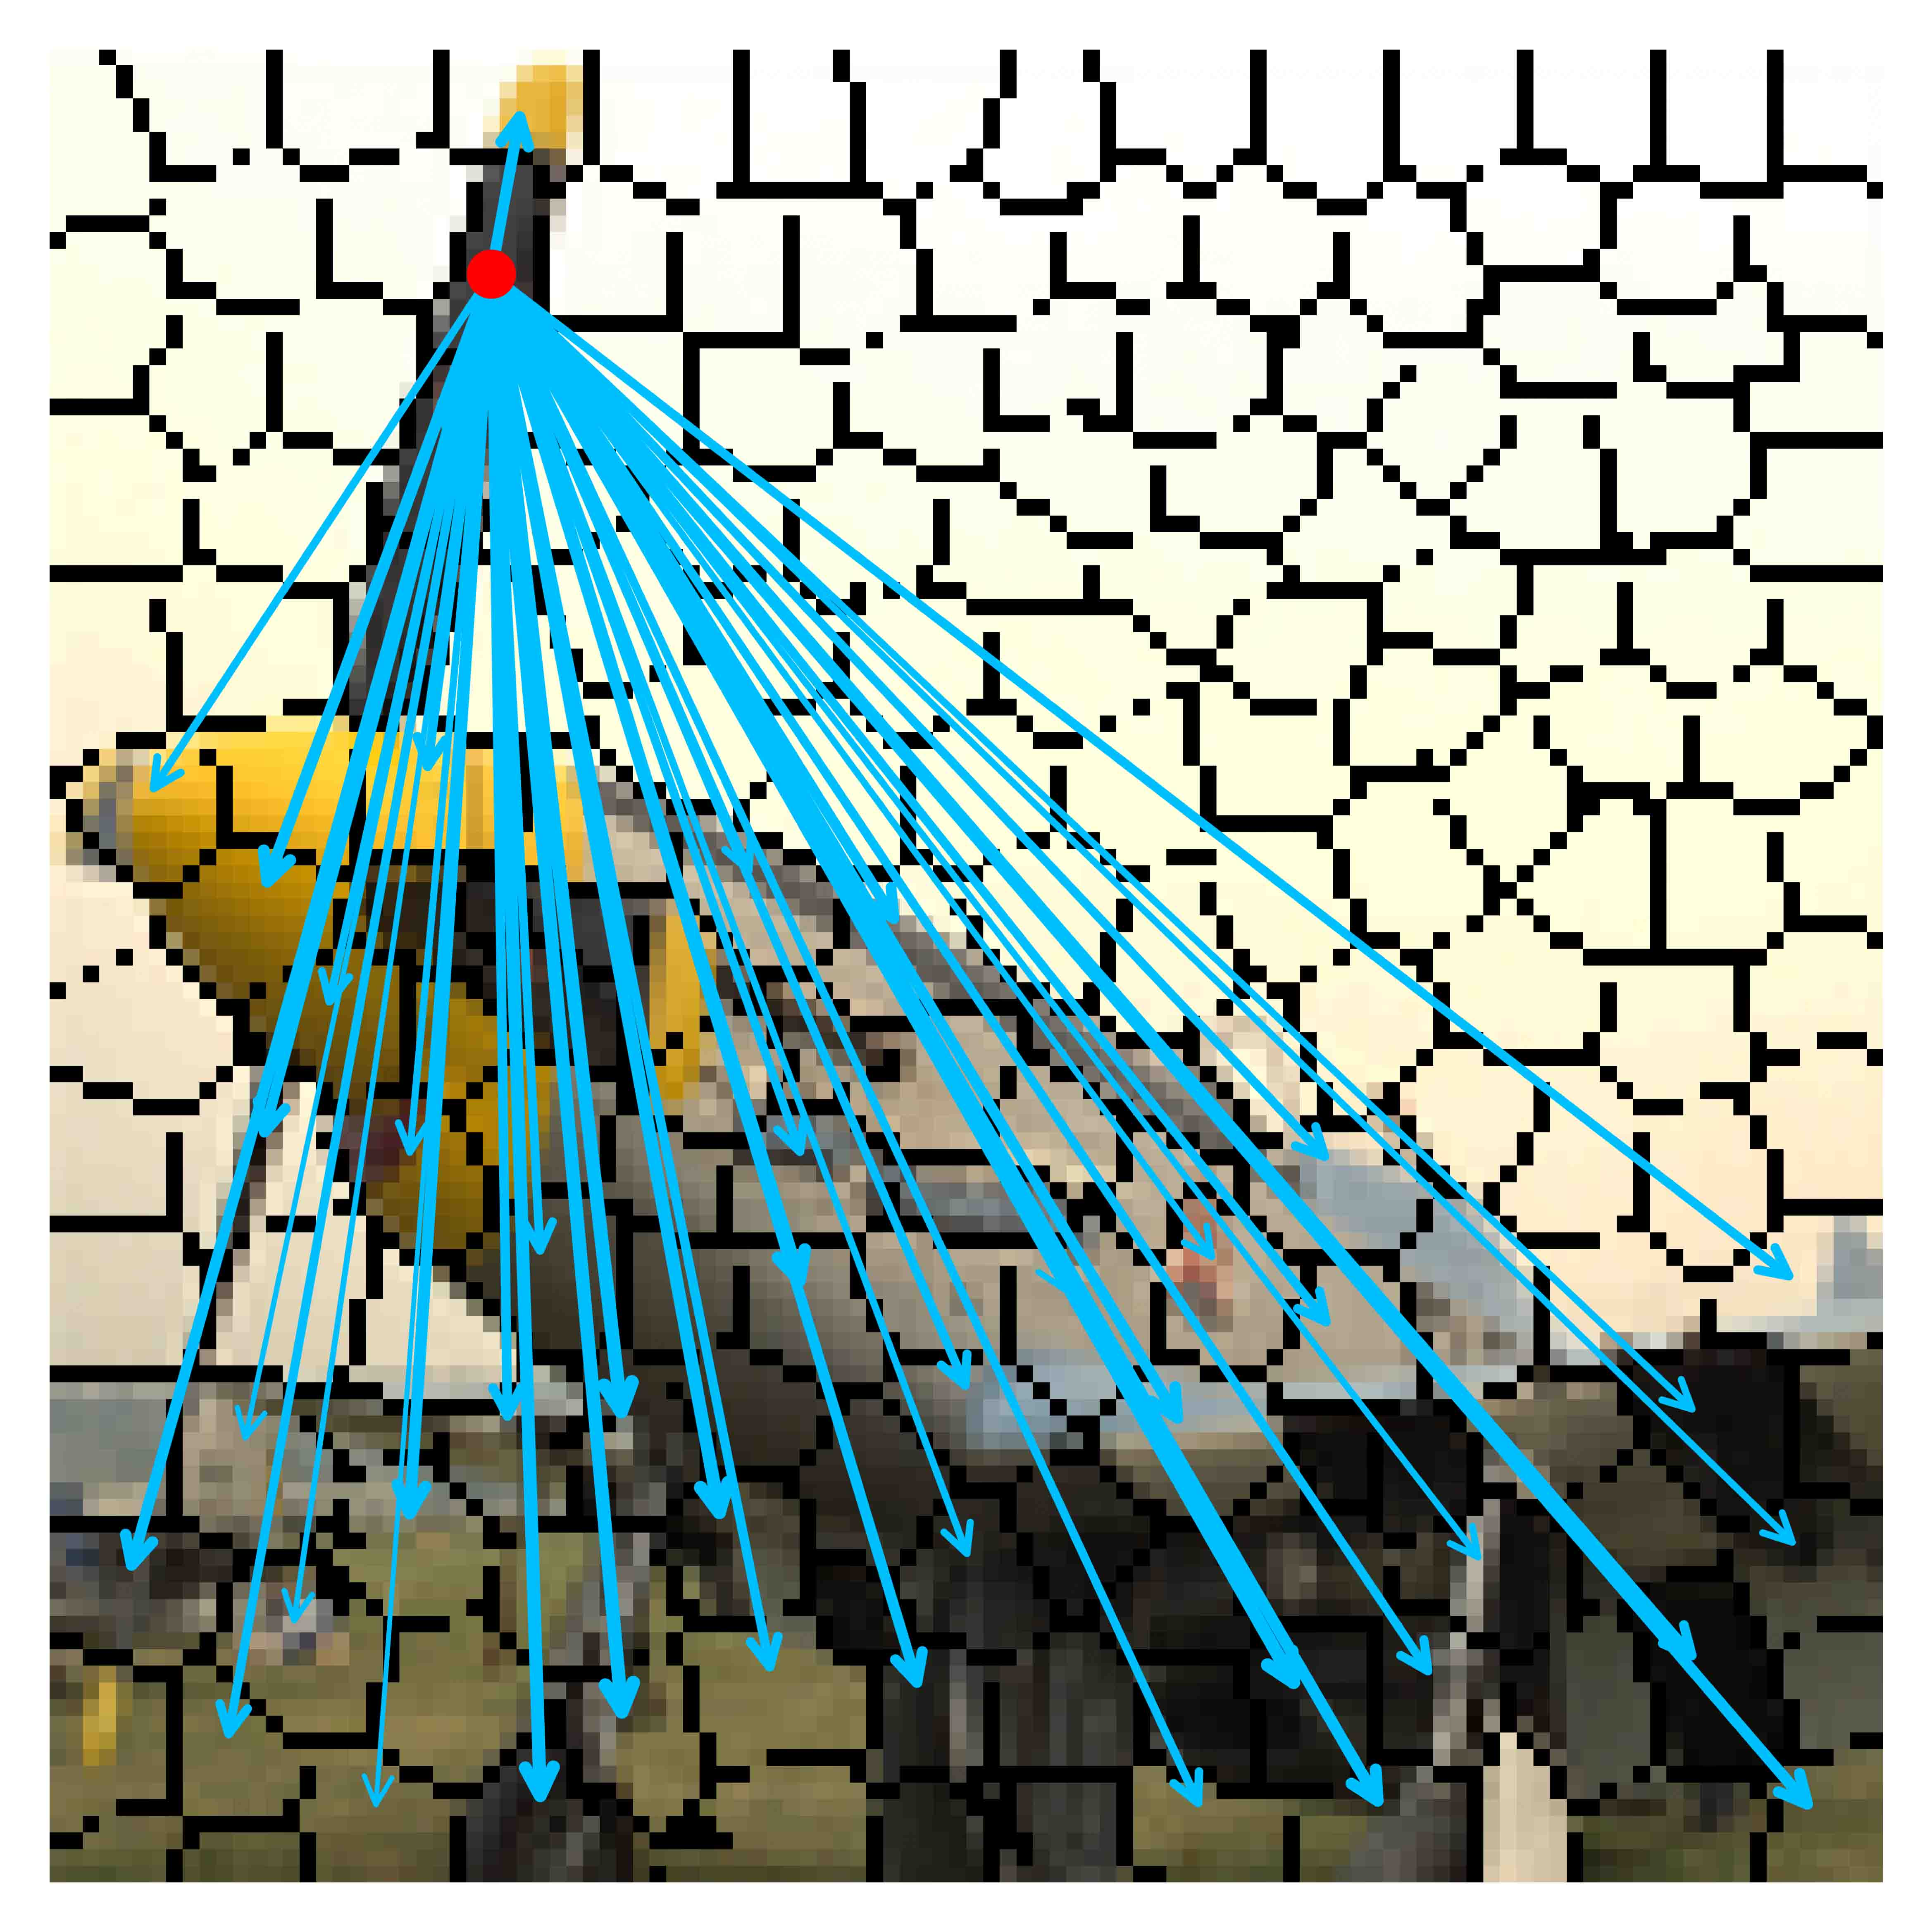
\includegraphics[width=2.8in]{images/jet_superpixel.jpg}
		\centerline{(a)}
		\label{JET}
	\end{minipage}
	\begin{minipage}[t]{.49\linewidth}
		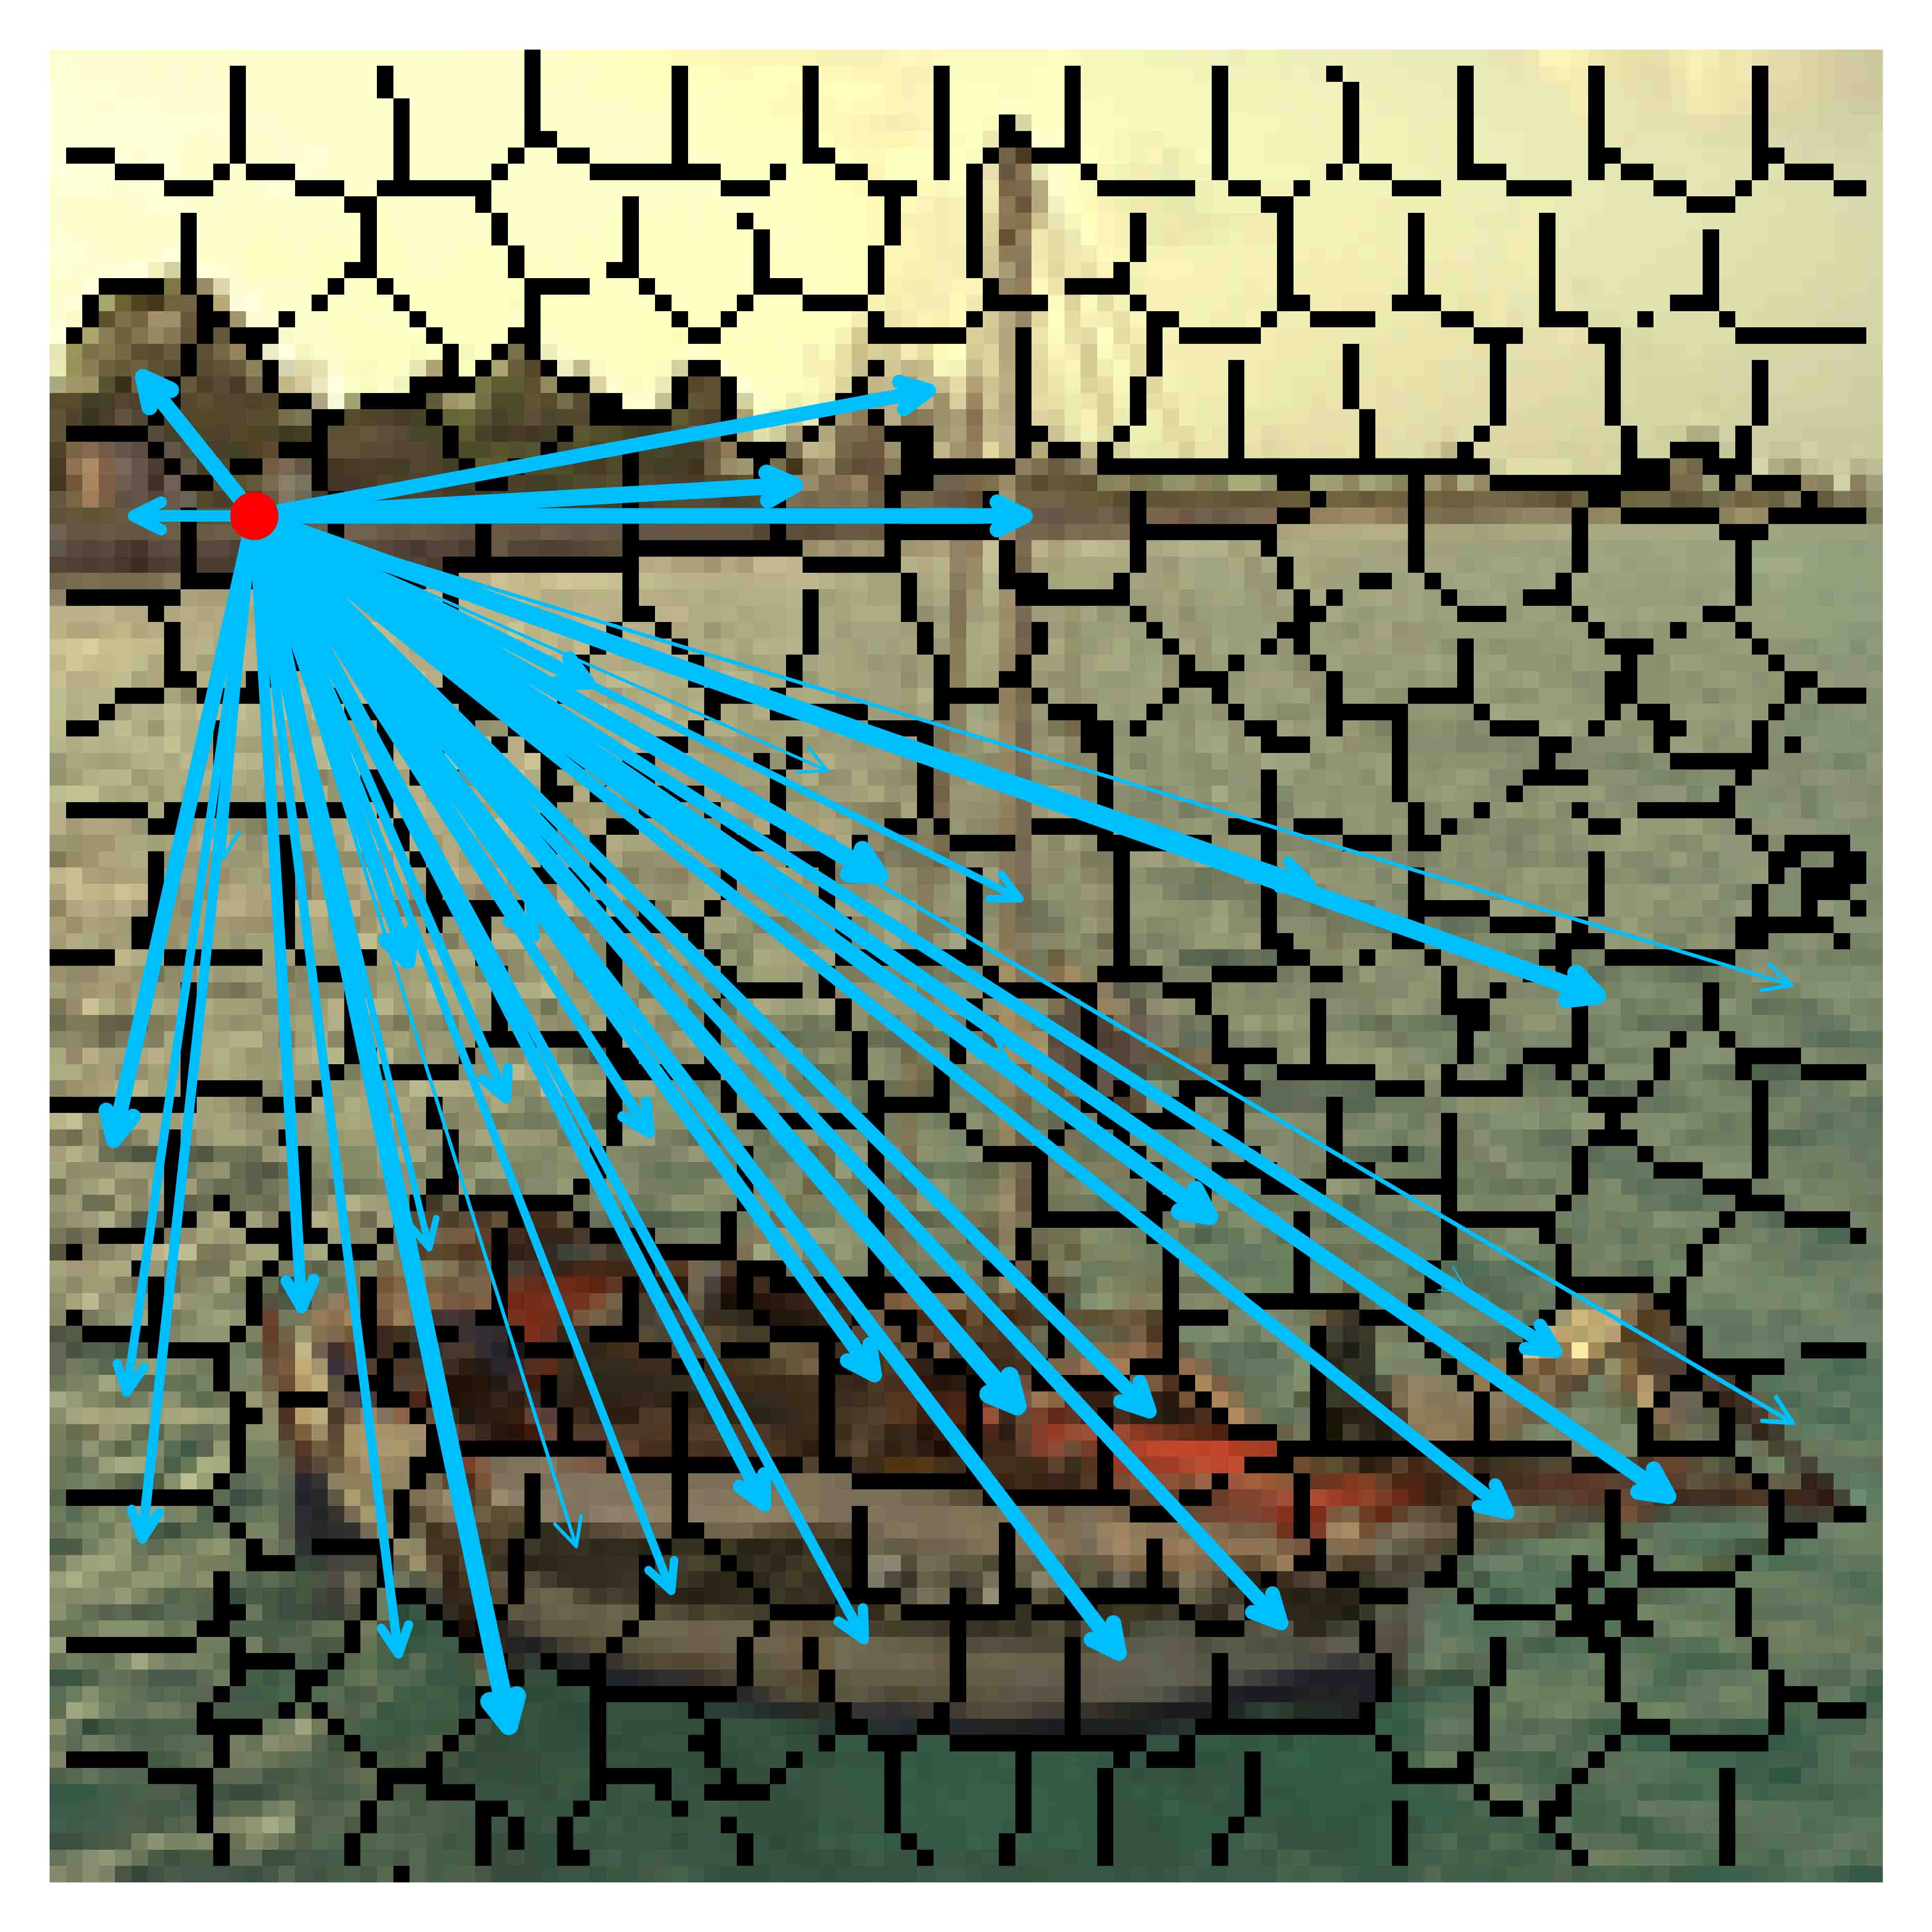
\includegraphics[width=2.8in]{images/I06_superpixel.jpg}
		\centerline{(b)}
		\label{BOAT}
	\end{minipage}
	\begin{minipage}[t]{.49\linewidth}
		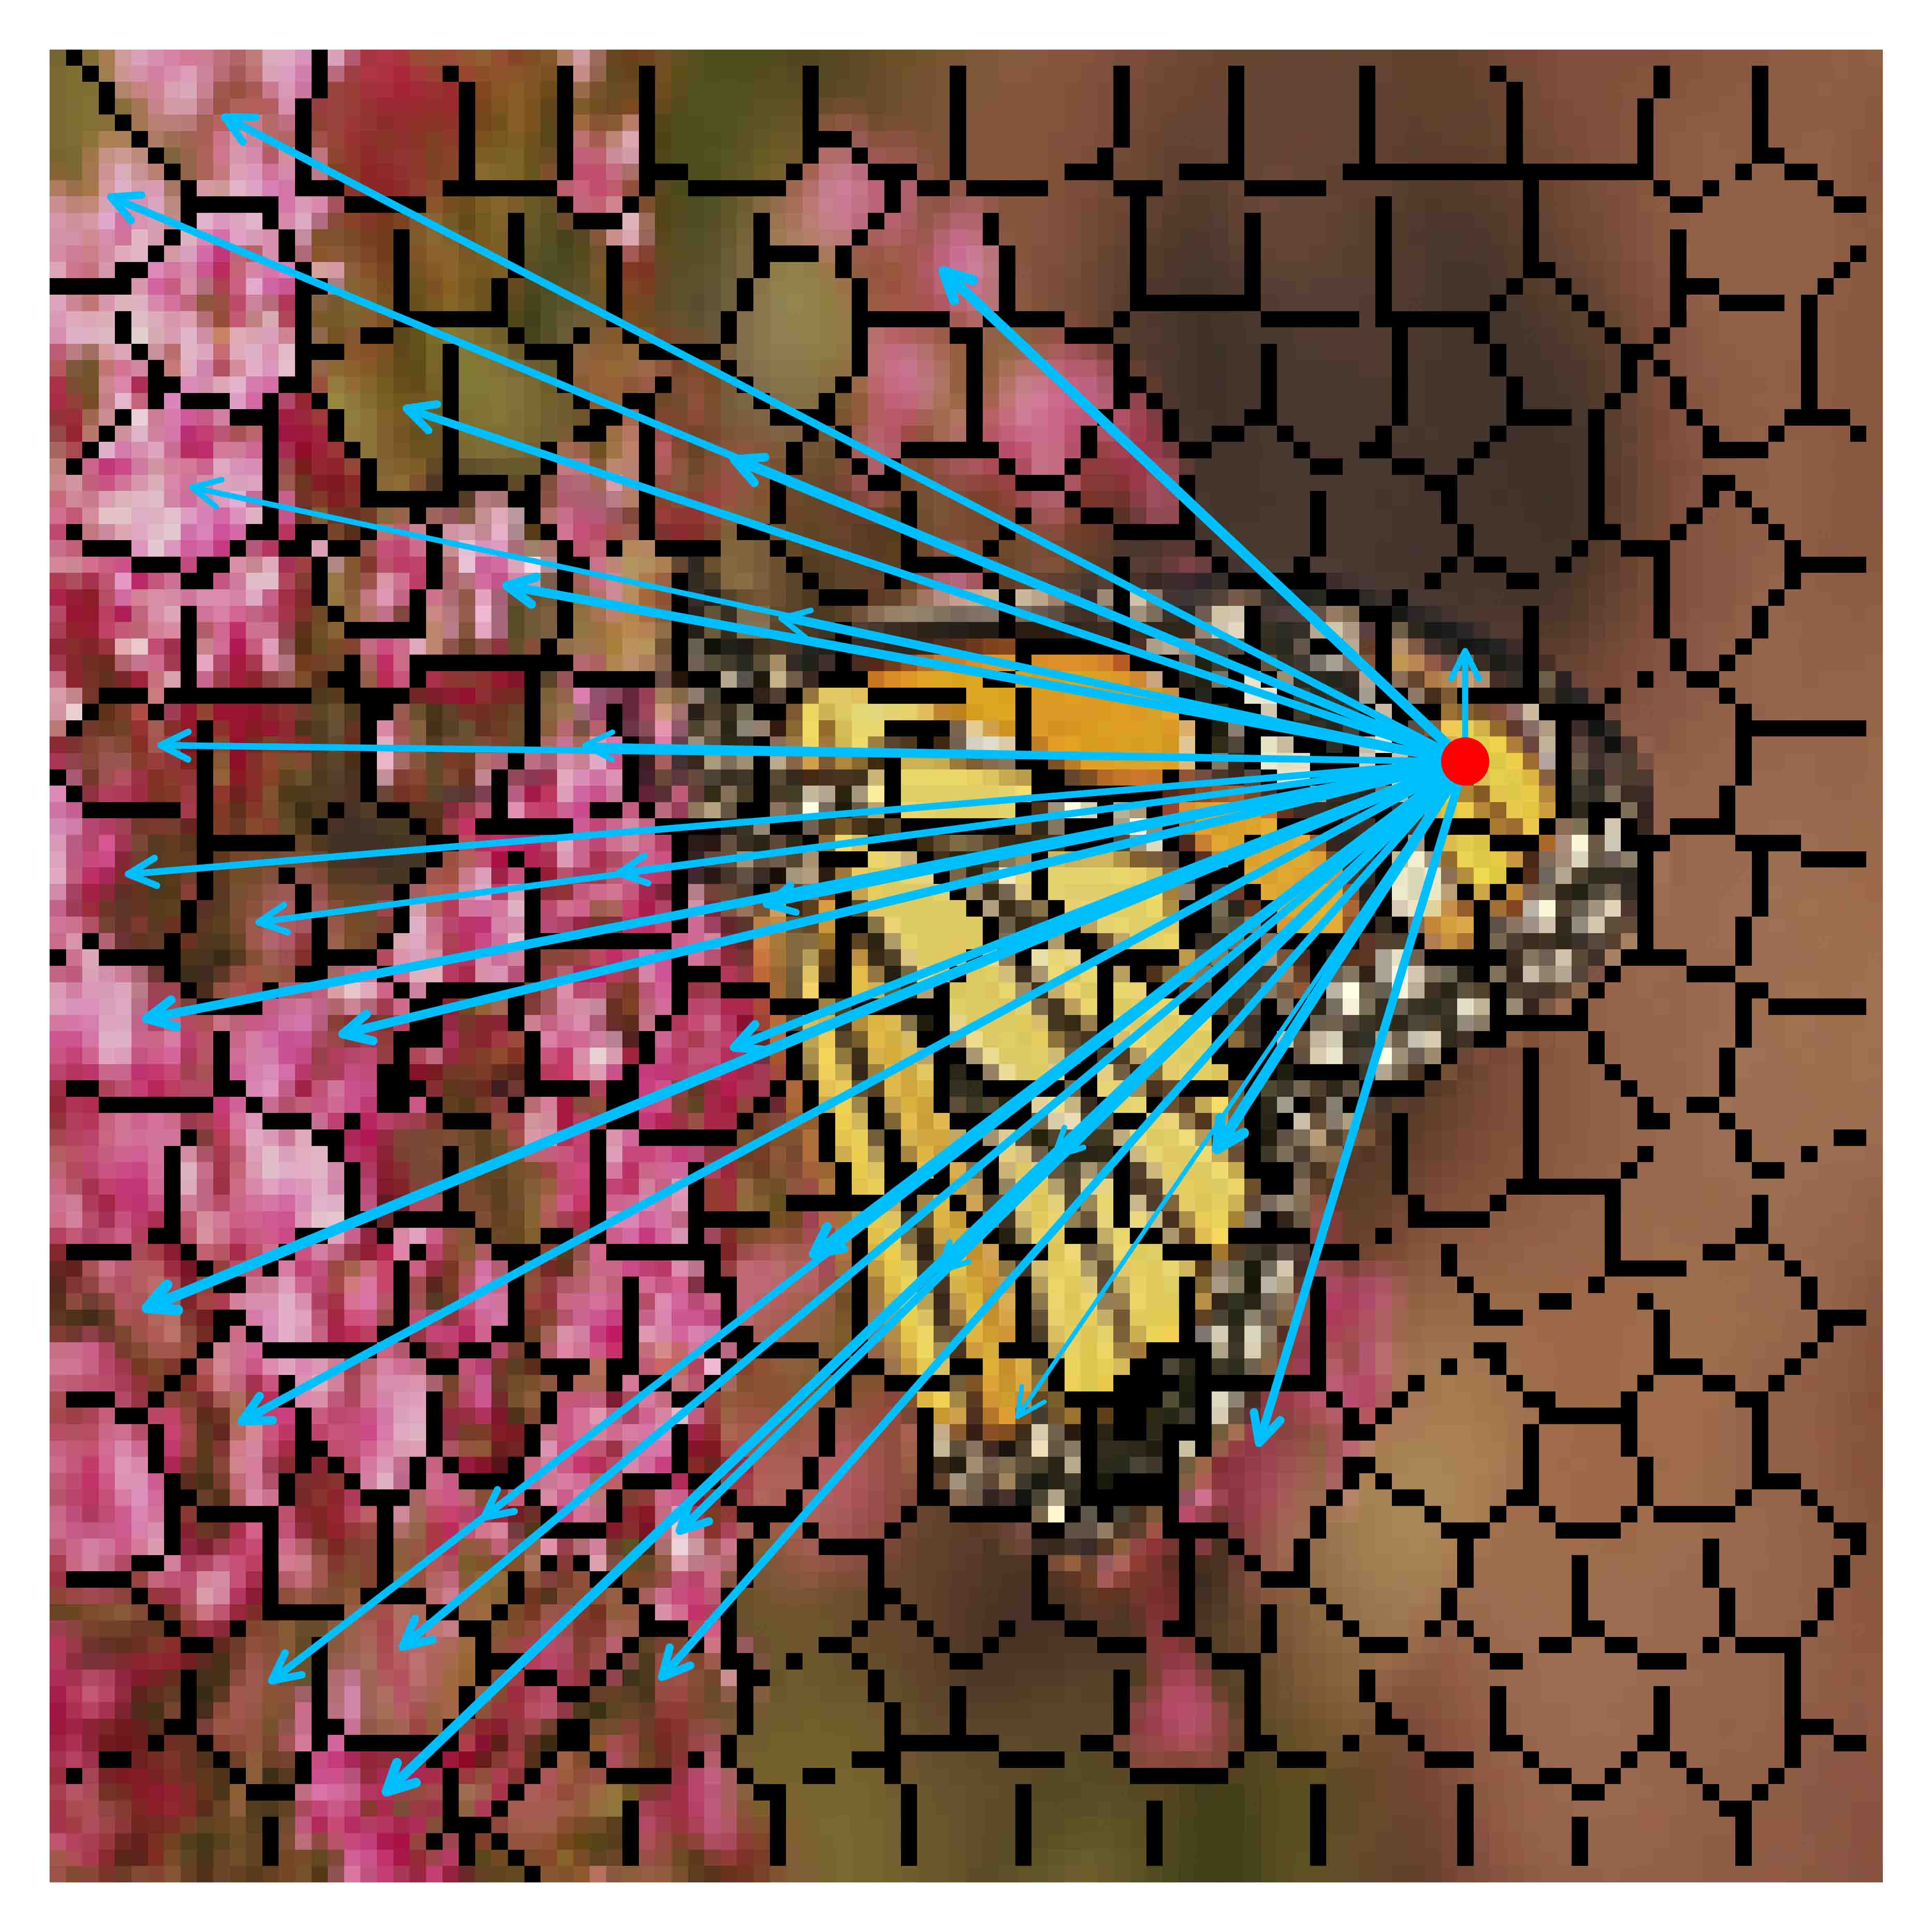
\includegraphics[width=2.8in]{images/monarch_superpixel.jpg}
		\centerline{(c)}
		\label{MONARCH}
	\end{minipage}
	\begin{minipage}[t]{.49\linewidth}
		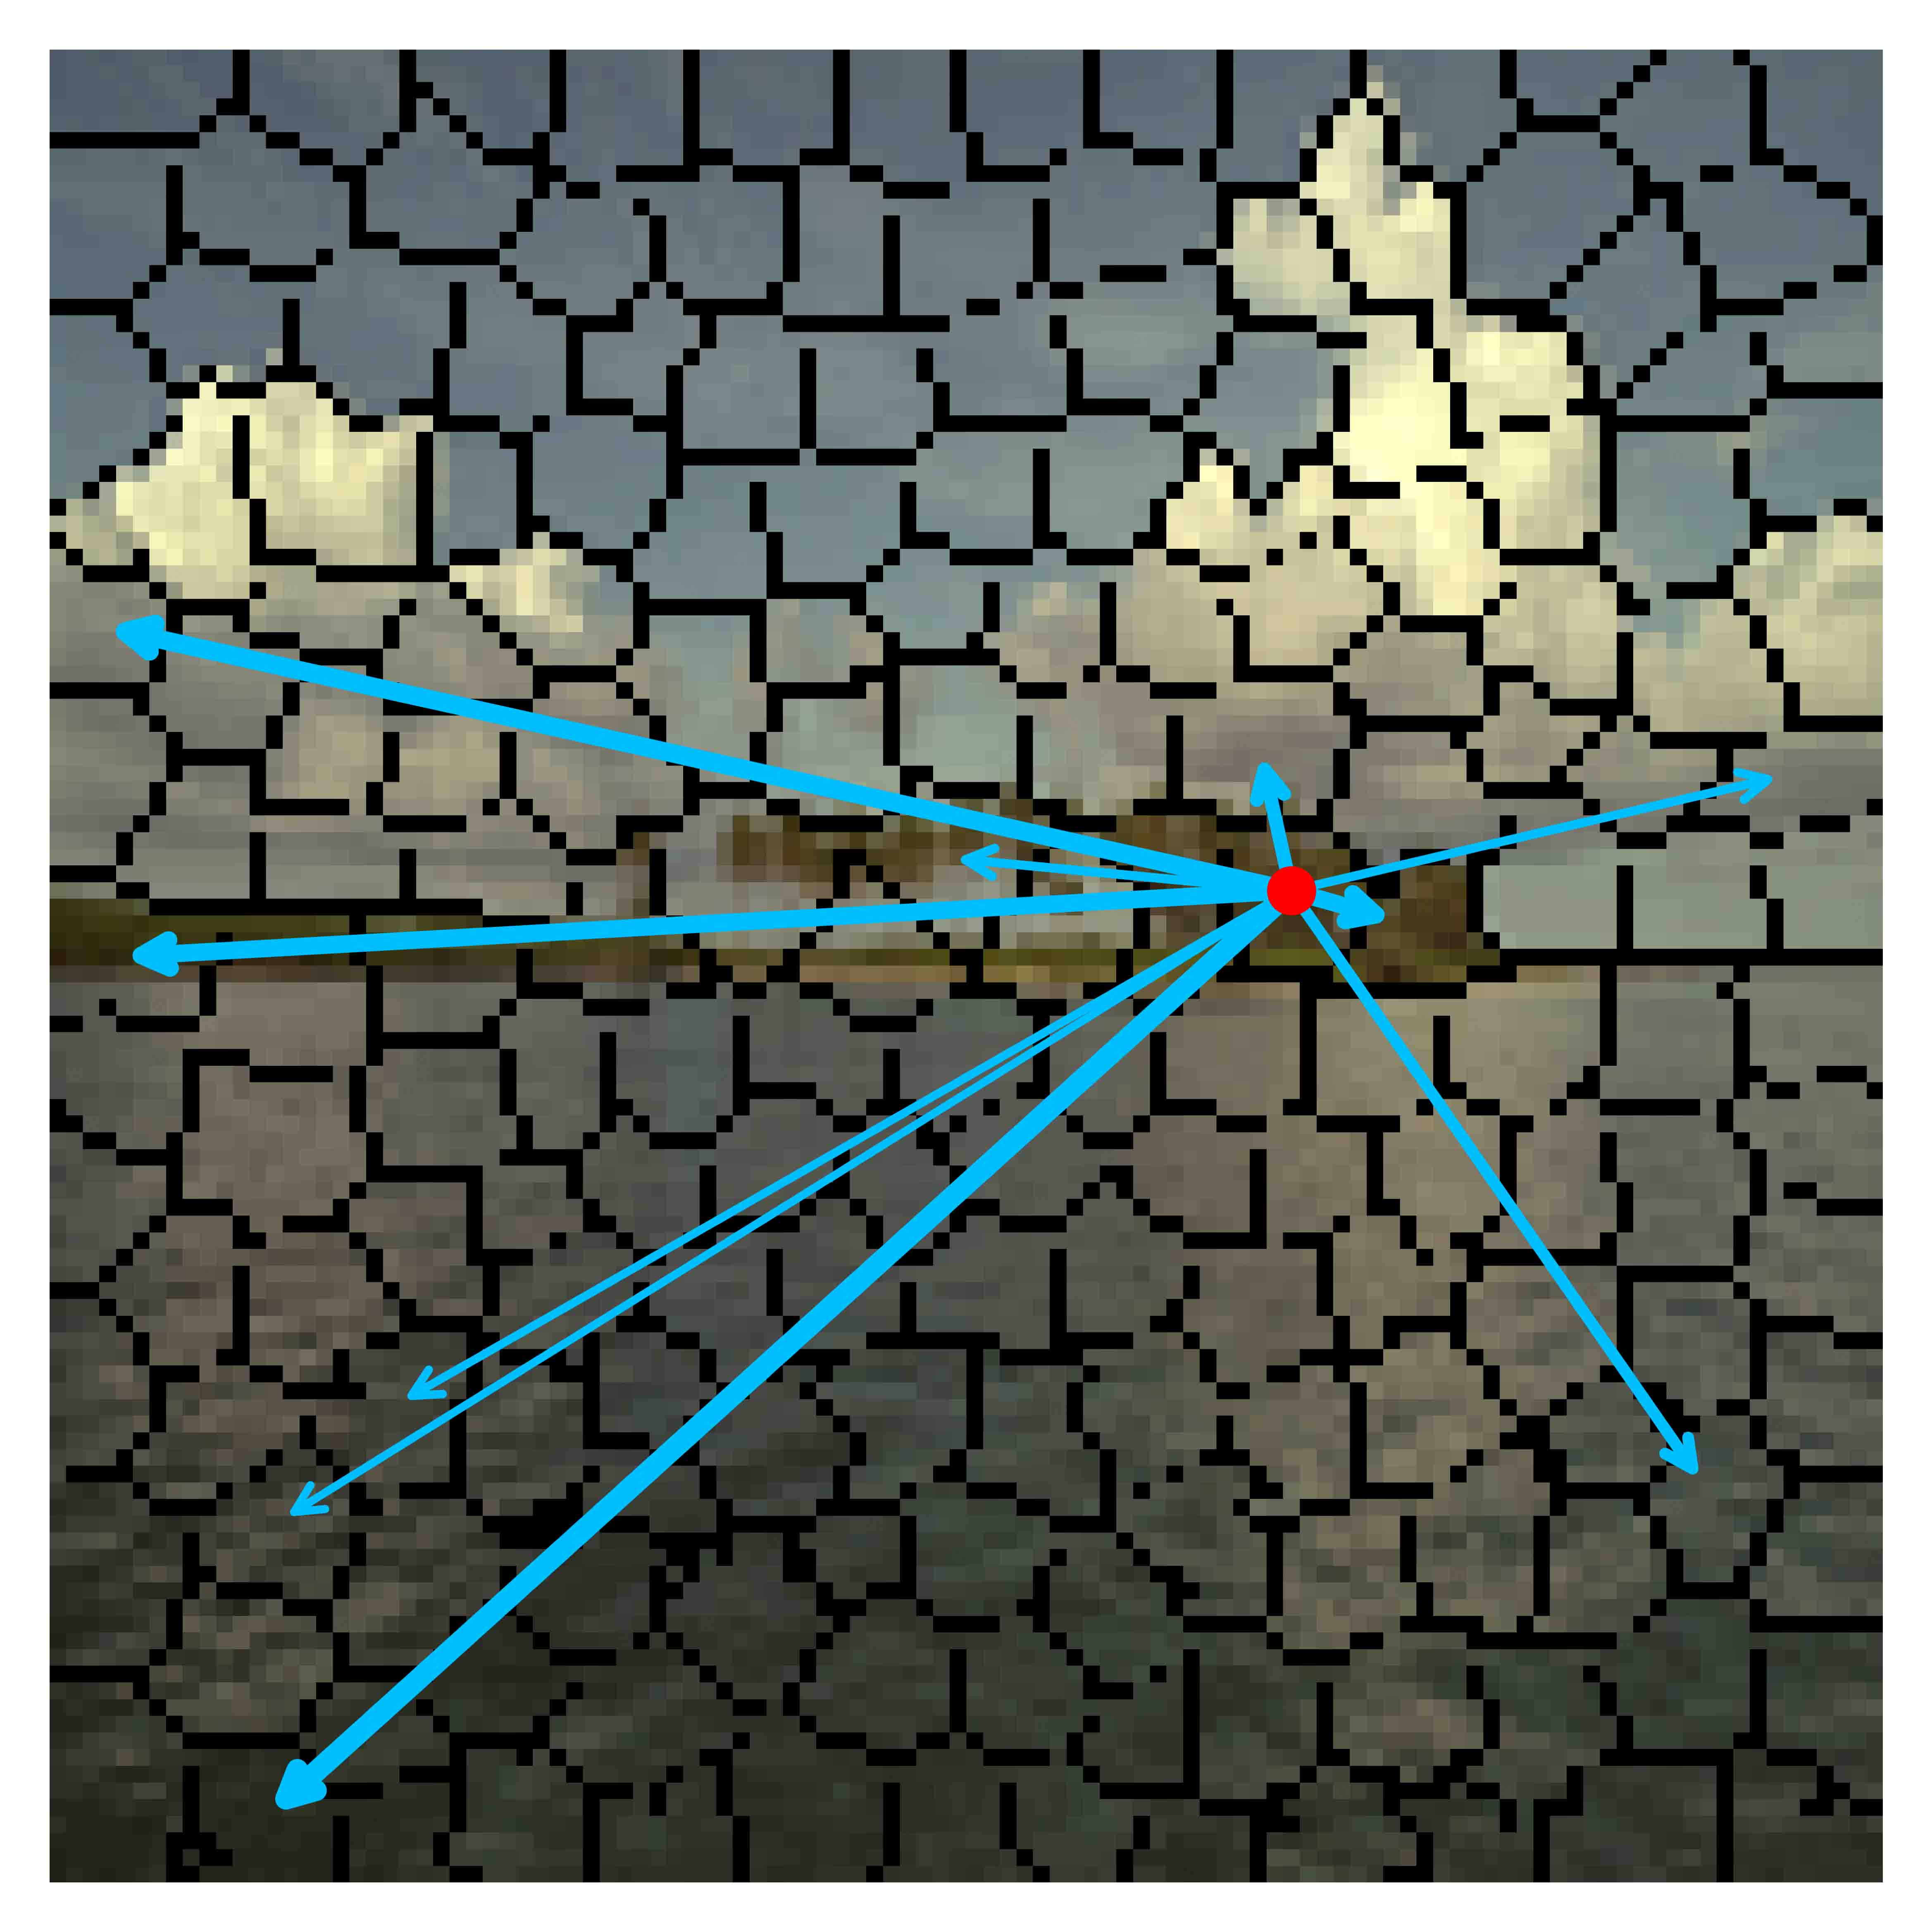
\includegraphics[width=2.8in]{images/ocean_superpixel.jpg}
		\centerline{(d)}
		\label{OCEAN}
	\end{minipage}
	\caption{Illustrations of the non-local behavior with superpixel segmentations. Images are randomly chosen from the TID2013 and LIVE databases for demonstrations. To verify the effectiveness of the non-local modeling and for better visibility, we resize the original image (\eg,~$384 \times 512$) to $112 \times 112$.}
	\label{Non-local Behavior from the TID2013 database with superpixel - 1}
\end{figure*}

We propose to extract the non-local features by GNN in a two-stage manner. In the first stage, a GNN layer is constructed to aggregate features within superpixels. In the second stage, the learned spatial features are integrated with a multi-head self-attention. We elaborate on the two stages as follows. 

In addition, in~\reffig{Non-local Behavior from the TID2013 database with superpixel - 1} and~\reffig{Non-local Behavior from the TID2013 database with superpixel - 2}, we illustrate some non-local behaviors with superpixel segmentations using some images from the TID2013, LIVE, and CSIQ databases. In detail, the figures are described as follows:~\reffig{Non-local Behavior from the TID2013 database with superpixel - 1}~(a) The plane image with a query on the wings.~\reffig{Non-local Behavior from the TID2013 database with superpixel - 1}~(b) The boat image with a query on the nearby river bank.~\reffig{Non-local Behavior from the TID2013 database with superpixel - 1}~(c) The butterfly image with a query on the wing.~\reffig{Non-local Behavior from the TID2013 database with superpixel - 1}~(d) The river image with a query on the riverbank.~\reffig{Non-local Behavior from the TID2013 database with superpixel - 2}~(a) The Statue of Liberty image with a query on the lady.~\reffig{Non-local Behavior from the TID2013 database with superpixel - 2}~(b) The shrooms image with a query on one shroom.~\reffig{Non-local Behavior from the TID2013 database with superpixel - 2}~(c) The Lafayette Square, Washington, D.C.~image with a query on one red flower.~\reffig{Non-local Behavior from the TID2013 database with superpixel - 2}~(d) The gecko image with a query on one gecko. Some of the results are analyzed and discussed in~\refsec{Non-local Dependency and Relational Modeling}.
\begin{figure*}[!ht]
	\centering
	\begin{minipage}[t]{.49\linewidth}
		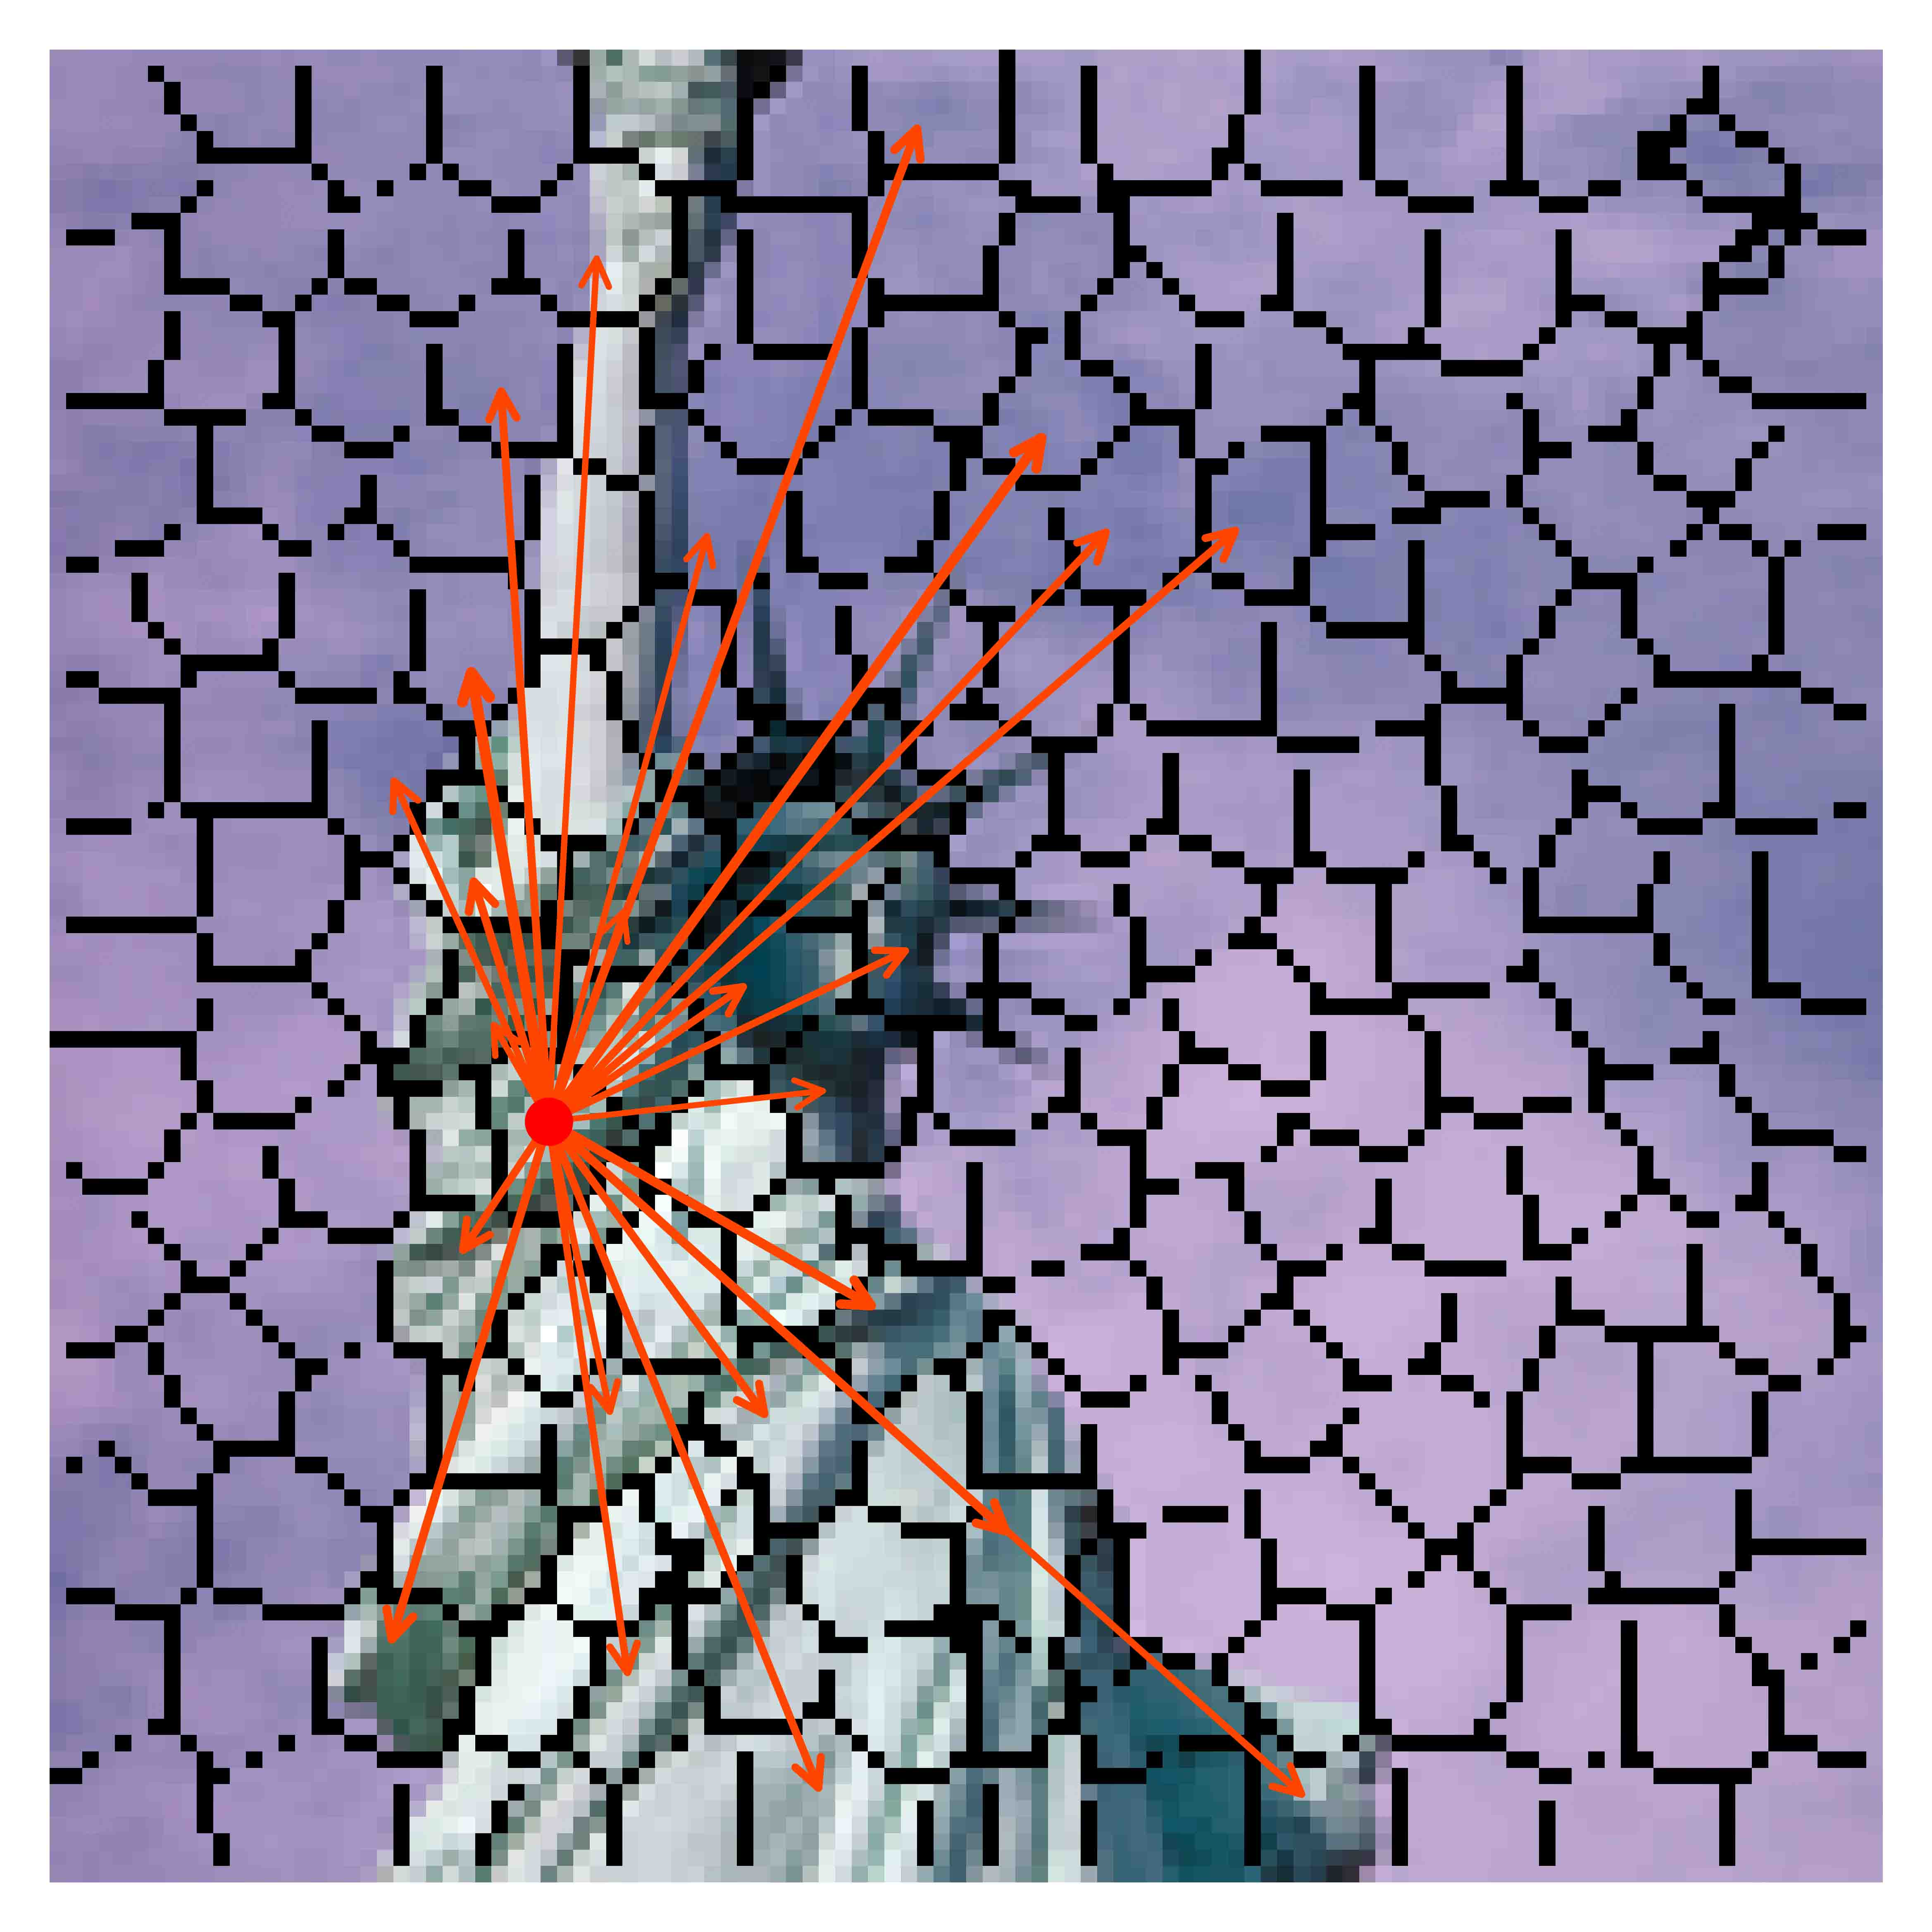
\includegraphics[width=2.8in]{images/lady_superpixel.jpg}
		\centerline{(a)}
		\label{LADY}
	\end{minipage}
	\begin{minipage}[t]{.49\linewidth}
		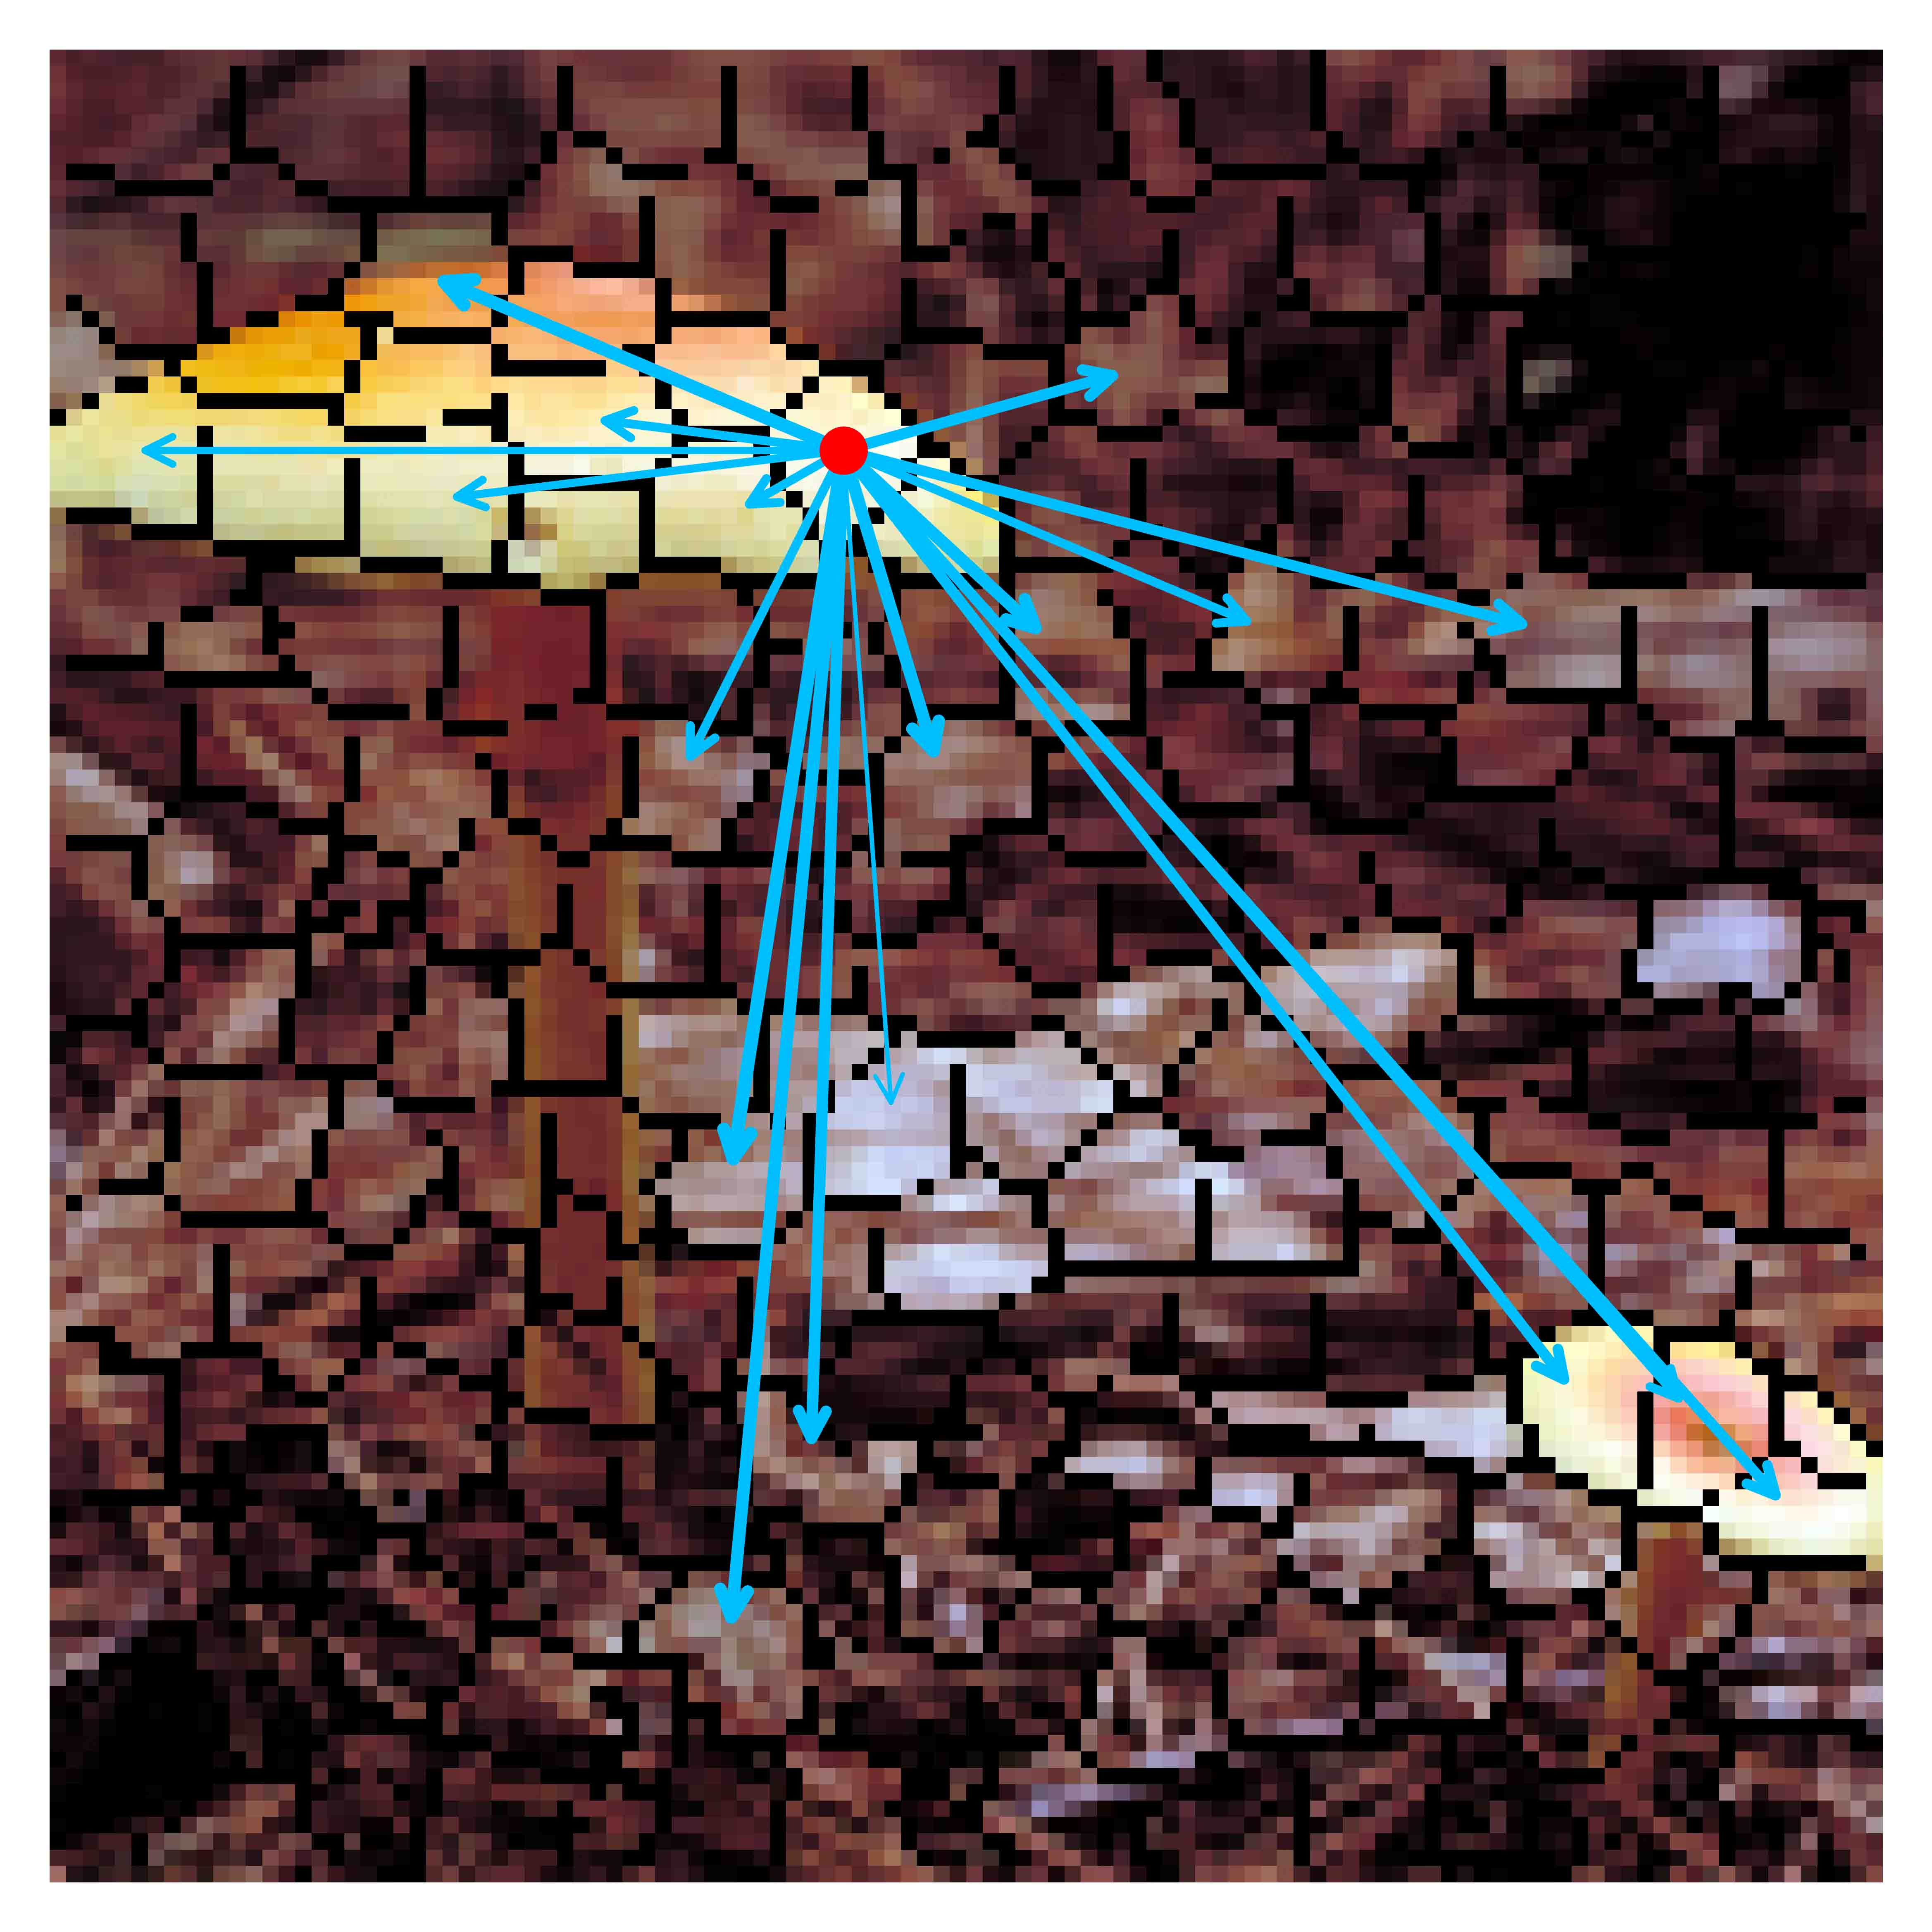
\includegraphics[width=2.8in]{images/shroom_superpixel.jpg}
		\centerline{(b)}
		\label{SHROOM}
	\end{minipage}
	\begin{minipage}[t]{.49\linewidth}
		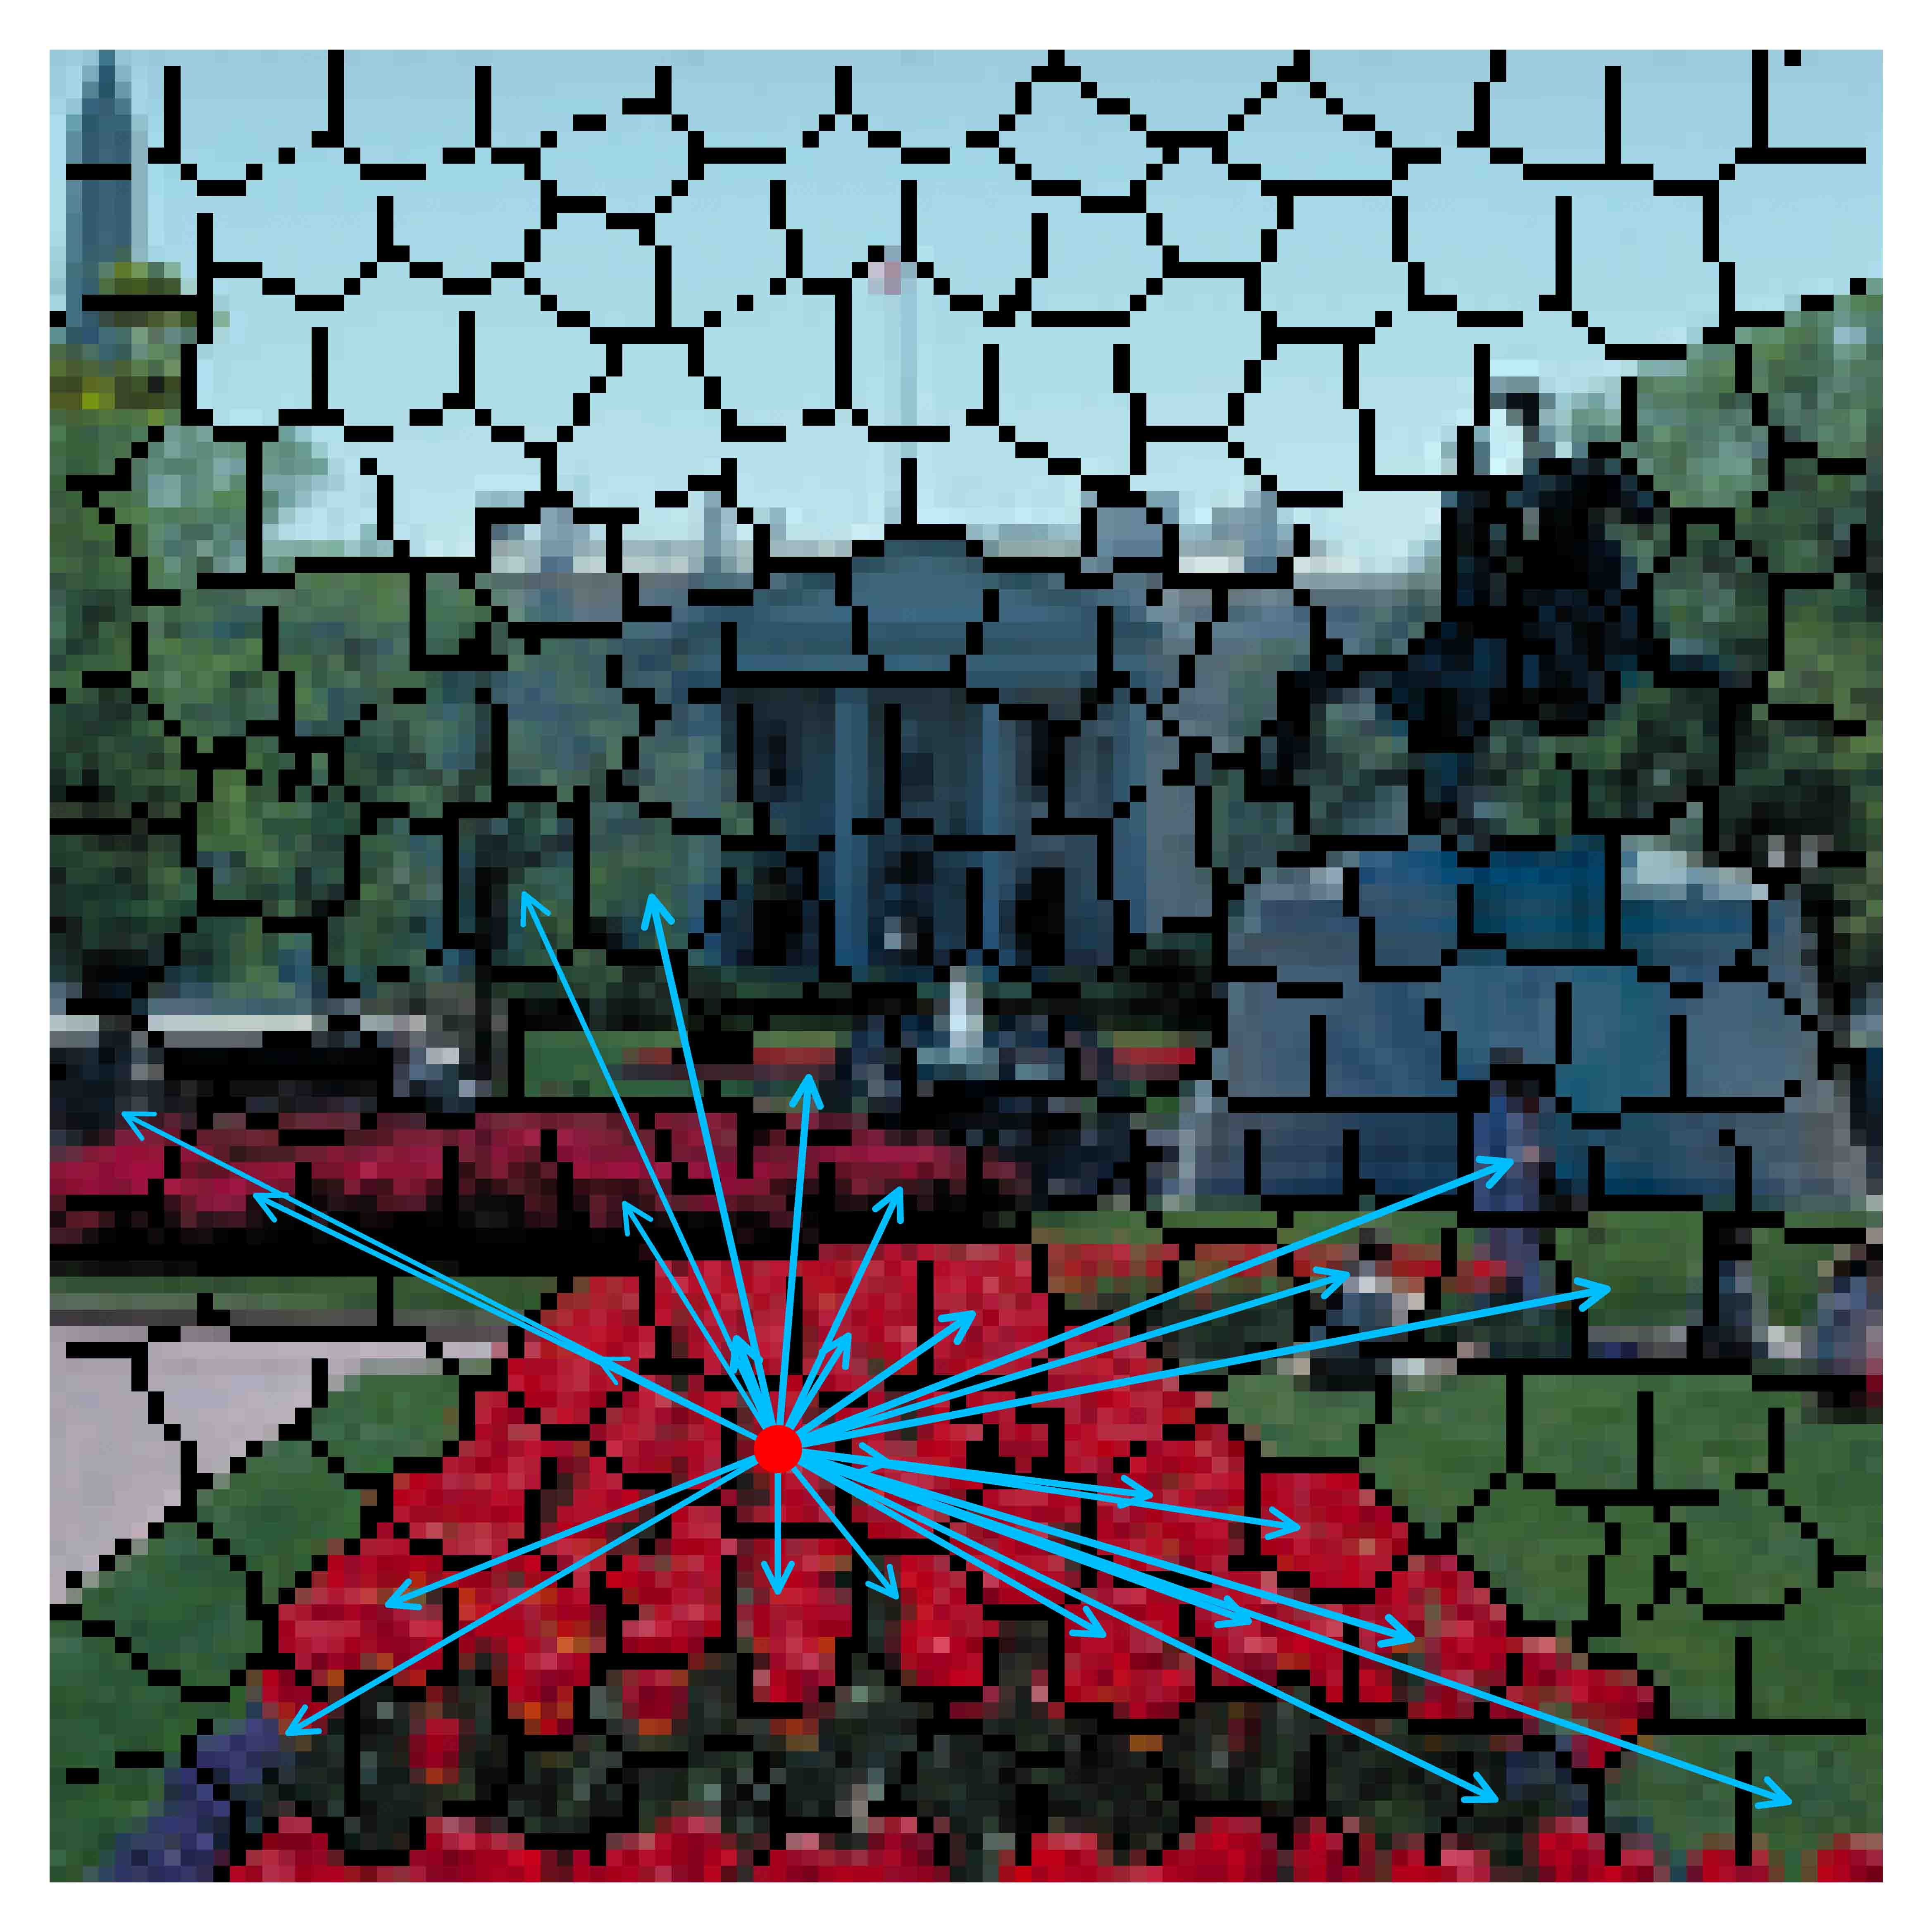
\includegraphics[width=2.8in]{images/flower_superpixel.jpg}
		\centerline{(c)}
		\label{FLOWER}
	\end{minipage}
	\begin{minipage}[t]{.49\linewidth}
		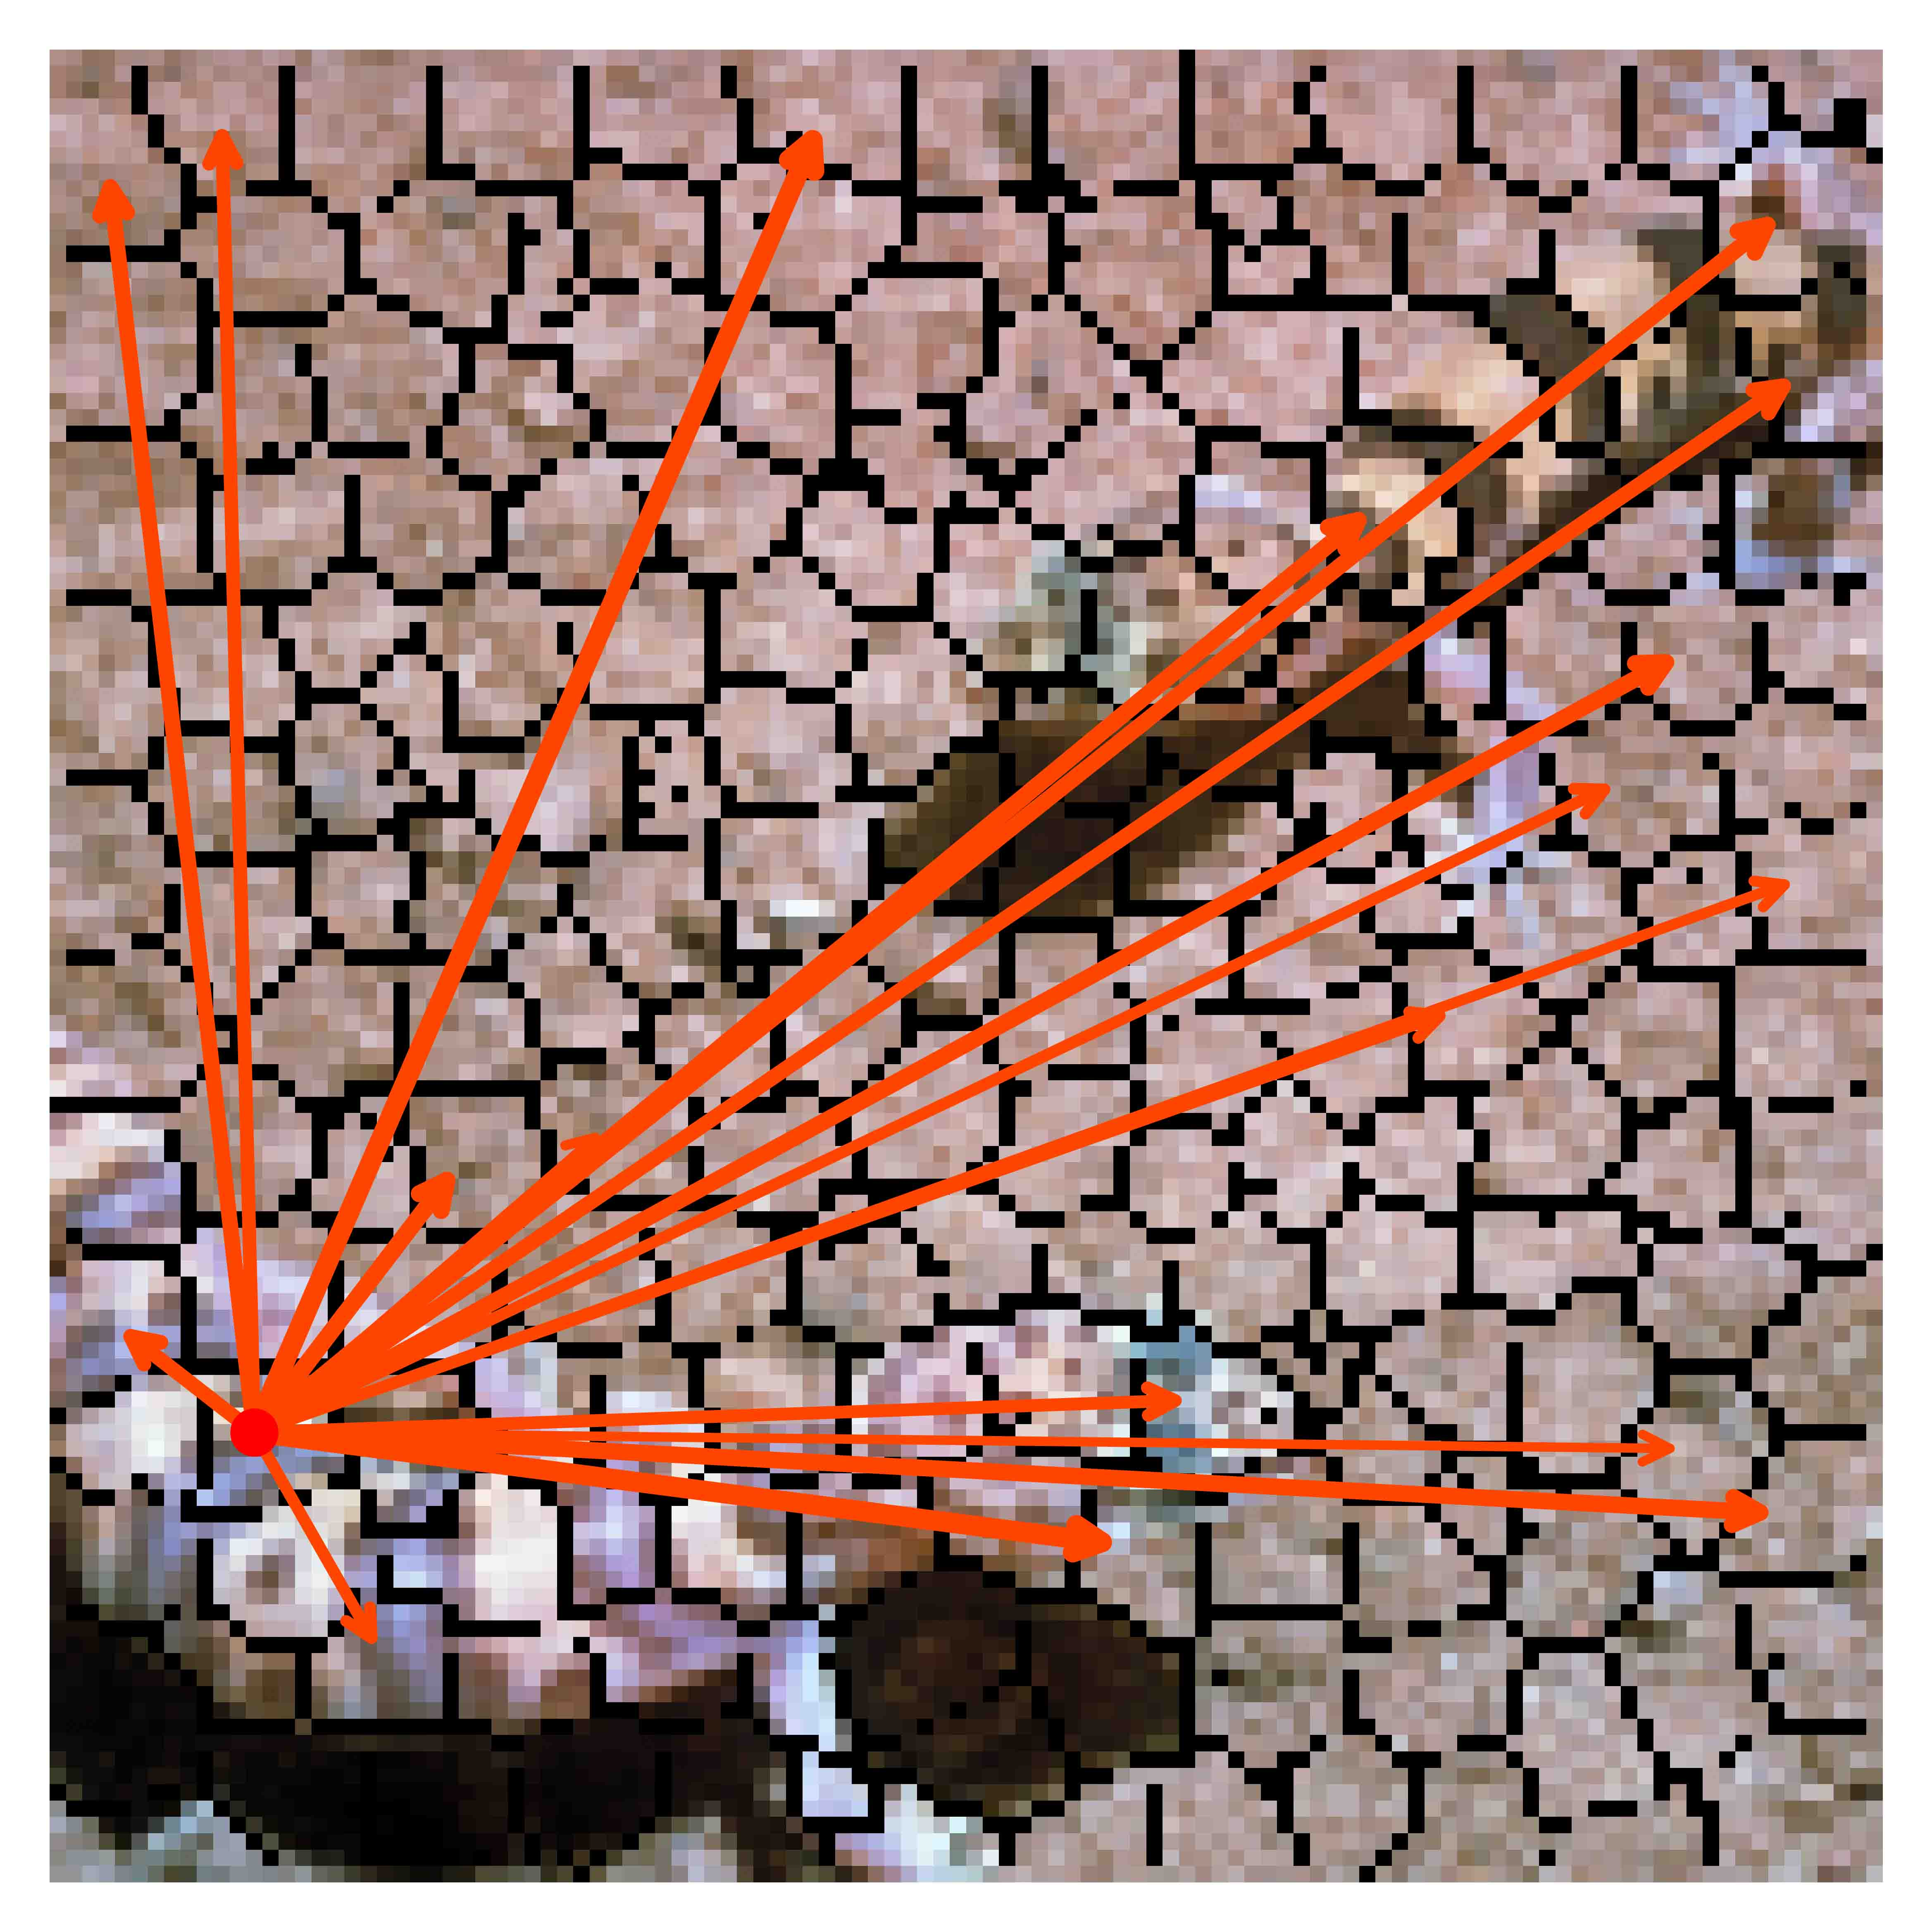
\includegraphics[width=2.8in]{images/geckos_superpixel.jpg}
		\centerline{(d)}
		\label{GECKOS}
	\end{minipage}
	\caption{Illustrations of the non-local behavior with superpixel segmentations. Images are randomly chosen from the CSIQ database for demonstrations. To verify the effectiveness of the non-local modeling and for better visibility, we resize the original image (\ie,~$512 \times 512$) to $112 \times 112$.}
	\label{Non-local Behavior from the TID2013 database with superpixel - 2}
\end{figure*}

\subsubsection{Graph Representation of Images}
There are four graph representations for images, from the perspectives of pixels, feature maps, groups of pixels, and images.
\paragraph{Pixel-level Representation}~Nodes $\boldsymbol{\mathrm{V}}$ of the graph are pixels as graph signals. Edges $\boldsymbol{\mathrm{E}}$ and adjacency matrix $\boldsymbol{\mathrm{A}}$ are pairs (denoting spatial proximity) between nodes. Because the spatial structure of images is regular in the Euclidean domain, images can be represented as regular spatial structures. Besides, it would be computationally inefficient and memory-intensive if all the image pixels were modeled as a graph. 

\paragraph{Feature Map-level Representation}~The second method is built upon feature maps. Graphs can be modeled inside these feature maps to learn the non-local information~\citep{wang2018non, yue2018compact, she2021hierarchical, zhang2019self, zhang2010non}. Although it may capture the non-local information from high-level semantic feature maps, it may be unable to extract low-level and middle-level features and statistics.

\paragraph{Group-level Representation}~The group-level representation gains much more attention nowadays due to the intrinsic properties of images' multi-scale and spatial-variant local regions. One way is to use square patches~\citep{dosovitskiy2020image, liu2021swin}. Another way is superpixels~\citep{Giraldo2022Graph}. The nodes of graph $\boldsymbol{\mathrm{V}}$ are superpixels in the image. Each superpixel's relative importance (correlation) is modeled by the adjacency matrix $\boldsymbol{\mathrm{A}}$.

\paragraph{Image-level Representation}~The last type is the image-level representation. For example, Sun~\etal model the relationships among image distortions by graphs~\citep{sun2022graphiqa}.

\subsubsection{Graph Construction}
Supposing $N$ superpixels are constructed by image segmentation, we construct an undirected and weighted graph denoted as $\boldsymbol{\mathrm{G}}$, and the superpixels are treated as nodes. Thus, $\boldsymbol{\mathrm{G}}=\{\boldsymbol{\mathrm{V}}, \boldsymbol{\mathrm{E}}, \boldsymbol{\mathrm{A}}\}$. In particular, $\boldsymbol{\mathrm{V}}$ denotes nodes (vertices), and $|\boldsymbol{\mathrm{V}}|=N$. $\boldsymbol{\mathrm{E}}$ denotes edges (links) that connect nodes $\boldsymbol{\mathrm{V}}$. The adjacency matrix $\boldsymbol{\mathrm{A}}$ contains weights (correlations) between nodes $\boldsymbol{\mathrm{V}}$.

\subsubsection{Self-Attention for Nodes Integration}
\begin{figure*}[!ht]
	\begin{minipage}[t]{\linewidth}
		\centering
		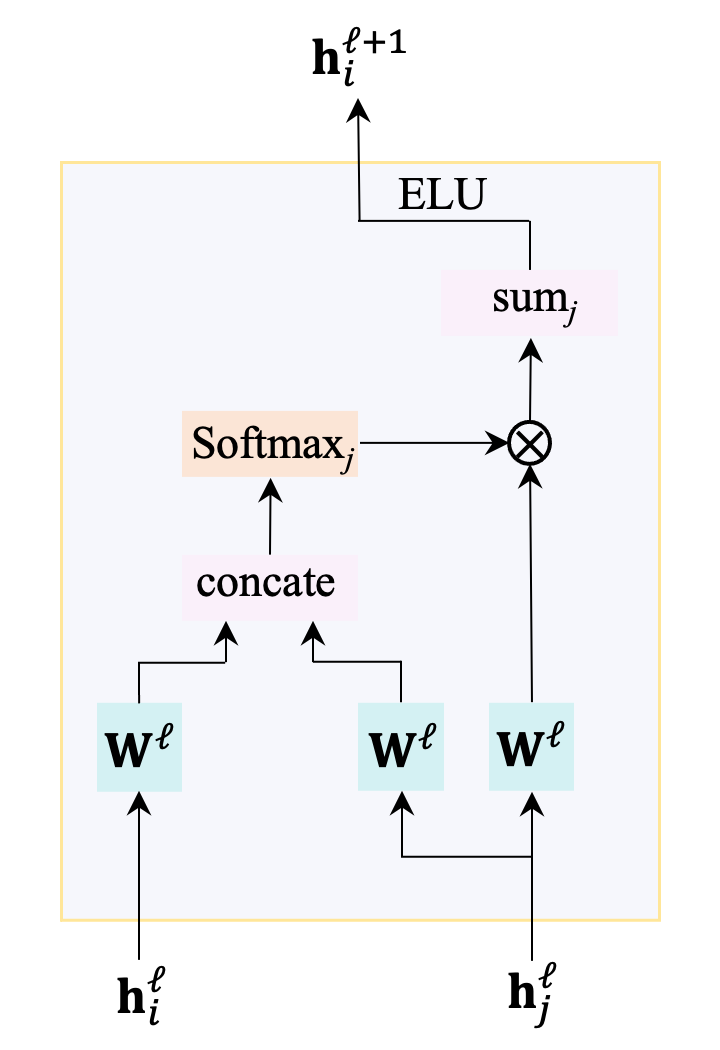
\includegraphics[width=2.5in]{fig/NLNet-Attention.png}
	\end{minipage}
	\caption{The demonstration of a self-attention module.}
	\label{NLNet}
\end{figure*}

To capture the long and short-range dependencies between different nodes, the self-attention mechanism is introduced in GNN. The demonstration of a self-attention module is shown in~\reffig{NLNet}.
\begin{equation}
	\boldsymbol{\mathrm{h}}_{i}^{l+1}=\mathrm{ELU}\left(\sum\limits_{j\in\mathcal{N}(i)} \alpha_{i j}^{l}\boldsymbol{\mathrm W}^{l} \boldsymbol{\mathrm h}_{j}^{l}\right),
	\label{GAT}
\end{equation}

\begin{equation}
	\mathrm{ELU}(\boldsymbol{\mathrm x})= \begin{cases}\boldsymbol{\mathrm x}, & \boldsymbol{\mathrm x}>0; \\ \alpha'(\exp(\boldsymbol{\mathrm x})-1), & \boldsymbol{\mathrm x} \leqslant 0.\end{cases}
	\label{ELU}
\end{equation}

\indent$\alpha_{i j}^{l}$ denotes the normalized attentional weight between node $j$ and node $i$ in the $l^{th}$ layer. Herein, $\mathcal{N}(i)$ is the neighborhood of the $i^{th}$ node, and $\boldsymbol{\mathrm h}_{j}^{l}$ are the features of the $j^{th}$ node in the $l^{th}$ layer. $\boldsymbol{\mathrm W}^{l}$ is a trainable matrix. We consider the Exponential Linear Unit (ELU)~\citep{clevert2015fast} as the activation function with $\alpha'=1$ and $\exp(\boldsymbol{\mathrm x})=e^{\boldsymbol{\mathrm x}}$. $\boldsymbol{\mathrm x}$ denote the input signals.

In~\refequ{GAT}, $\alpha_{i j}^{l}$ can be computed via a Softmax function~\citep{bridle1989training}.
\begin{equation}
	\alpha_{i j}^{l}=\frac{\mathrm{exp}\left(a_{i j}^{l}\right)}{\sum\limits_{k \in \mathcal{N}(i)} \mathrm{exp}\left(a_{i k}^{l}\right)},
	\label{softmax}
\end{equation}

\begin{equation}
	a_{i j}^{l}=\mathrm{LeakyReLU}\left({\mathrm{FC}}\left(\left[\boldsymbol{\mathrm W}^{l} \boldsymbol{\mathrm h}_{i}^{l} \| \boldsymbol{\mathrm W}^{l} \boldsymbol{\mathrm h}_{j}^{l}\right]\right)\right),
	\label{concat}
\end{equation}

\begin{equation}
	\mathrm{LeakyReLU}(\boldsymbol{\mathrm x})= \begin{cases}\boldsymbol{\mathrm x}, & \boldsymbol{\mathrm x}>0; \\ \alpha'' \boldsymbol{\mathrm x}, & \boldsymbol{\mathrm x} \leqslant 0.\end{cases}
	\label{LeakyReLU}
\end{equation}

\indent$a_{i j}^{l}$ is an attentional coefficient representing the importance of node $j$ to the center node $i$. $a_{i j}^{l}$ is derived by the concatenation of the mapped features $\boldsymbol{\mathrm W}^{l} \boldsymbol{\mathrm h}_{i}^{l}$ and $\boldsymbol{\mathrm W}^{l} \boldsymbol{\mathrm h}_{j}^{l}$ with a fully-connected neural network ${\mathrm{FC}}(\cdot)$. The Leaky Rectified Linear Unit (Leaky ReLU, denoted as $\mathrm{LeakyReLU}$ in~\refequ{LeakyReLU})~\citep{maas2013rectifier} is considered here as the activation function with $\alpha''=0.2$. We further adopt the multi-head self-attention mechanism for stable training~\citep{velickovic2018graph}.

\begin{equation}
	\boldsymbol{\mathrm h}_{i}^{l+1}=\mathop{\|}\limits_{m=1}^{M} \mathrm{ELU}\left(\sum_{j\in\mathcal{N}_{i}} \alpha_{i j}^{l, m} \boldsymbol{\mathrm W}^{l, m} \boldsymbol{\mathrm h}_{j}^{l}\right),
\end{equation}
where $M$ is the number of heads. It should be noted that although the learnable weight $\boldsymbol{\mathrm W}^{l, m}$ is shared among nodes, the graph attention layer aggregates features of each node with distinctions via different attentional coefficient $\alpha_{i j}^{l, m}$~\citep{velickovic2018graph}, highly improving the learning capacity of the GNN. After the aggregation, we normalize the acquired features of each node to alleviate the variance inflammation and prevent gradient vanishing~\citep{zhou2021understanding} as follows,

\begin{equation}
	\text{NodeNorm}\left(\boldsymbol{\mathrm x}_{i}\right)=\frac{x_{i, j}}{\left\{\left(\frac{1}{F-1}\sum_{j=1}^F (x_{i, j}-\bar{{x}}_i)^2\right)^{1/2}\right\}^{1/p} + C'}.
	\label{nodenorm}
\end{equation}

\indent$\boldsymbol{\mathrm x}_i \in\mathbb{R}^{1 \times F}$ represents graph signals of the $i^{th}$ node. $x_{i, j}$ denotes the $j^{th}$ feature of the $i^{th}$ node, and ${\bar{x}}_{i}=\sum_{j=1}^F x_{i, j}/F$ is the standard deviation of features in the $i^{th}$ node. $p$ is a constant, and $C'$ is a small positive constant to stabilize training. Finally, the means and standard deviations of the deep visual features are obtained from the graph attention layers,

\begin{equation}
	{\mu}_{j}=\frac{1}{N} \sum_{i=1}^{N} x_{i, j},
\end{equation}

\begin{equation}
	{\sigma_{j}}=\left(\frac{1}{N-1} \sum_{i=1}^{N}\left({x}_{i, j}-{\mu_{j}}\right)^{2}\right)^{\frac{1}{2}},
\end{equation}
in which $\boldsymbol{\mathrm{\mu_x}}=[{\mu}_{1},\cdots,{\mu}_{F}]\in\mathbb{R}^{1 \times F}$ denote the mean intensities of each graph feature layer, and $\boldsymbol{\mathrm{\sigma_{x}}}=[\sigma_{1},\cdots,\sigma_{F}]\in\mathbb{R}^{1 \times F}$ represent the standard deviations of features. By combining the feature means $\boldsymbol{\mathrm{\mu_{x}}}$ and standard deviations $\boldsymbol{\mathrm{\sigma_{x}}}$ along the feature dimension, the non-local features $\boldsymbol{\mathrm{f_{n}}}$ are extracted for the overall image quality estimation.

\subsection{Local Modeling via CNN}
In addition to the non-local features $\boldsymbol{\mathrm{f_{n}}}$ learned by the GNN, we further adopt the VGGNet-16 which is pre-trained on the ImageNet~\citep{deng2009imagenet} as the backbone for local feature extraction. As it is trained on the ImageNet database and focuses on the high-level vision tasks,~\eg, image classification and object detection, ideally, such a model is sensitive to high-level semantic information but robust to image distortions~\citep{wu2020end}. However, IQA models should be sensitive to semantic information and distortions. Besides, image quality degradation is hierarchical, which is consistent with the hierarchical degradation process of HVS~\citep{wu2020end}. Image features are degraded from the low-level local details, middle-level regional patterns to the high-level global abstracts. Therefore, feature maps from different layers are used to represent local features of the overall image quality. Thus, we employ the pre-trained VGGNet-16 to initialize the learnable parameters and fine-tune it with an image quality-related database~\citep{dingIQA}. In particular, we discard the fully-connected layers, and the multi-scale features at five stages are utilized. We denote the extracted local features as $\boldsymbol{\mathrm{f_{l}}}$.
\begin{equation}
	\boldsymbol{\mathrm{f_{l}}}=\mathop{\|}\limits_{i=1}^{5} \boldsymbol{\mathrm{f_{i}}}.
\end{equation}

\indent Furthermore, feature mean intensities and standard deviations are derived from the hierarchical feature maps $\boldsymbol{\mathrm{f_{l}}}$. For individual feature maps $\boldsymbol{\mathrm{f_{i}}}$, they hold 64 ($\boldsymbol{\mathrm{f_{1}}}$), 128 ($\boldsymbol{\mathrm{f_{2}}}$), 256 ($\boldsymbol{\mathrm{f_{3}}}$), 512 ($\boldsymbol{\mathrm{f_{4}}}$), 512 ($\boldsymbol{\mathrm{f_{5}}}$) feature maps, respectively. The mean intensities $\boldsymbol{\mathrm\mu}_{\boldsymbol{\mathrm{f_{i}}}}$ of feature maps $\boldsymbol{\mathrm{f_{i}}}$ can be described as:

\begin{equation}
	\boldsymbol{\mathrm\mu}_{\boldsymbol{\mathrm{f_{i}}}}=\frac{1}{H_{\boldsymbol{\mathrm{f_{i}}}} \times W_{\boldsymbol{\mathrm{f_{i}}}}} \sum_{i=1}^{H_{\boldsymbol{\mathrm{f_{i}}}}} \sum_{j=1}^{W_{\boldsymbol{\mathrm{f_{i}}}}} \boldsymbol{\mathrm{f_{i}}}\left(i, j\right),
\end{equation}
where $H_{\boldsymbol{\mathrm{f_{i}}}}$ and $W_{\boldsymbol{\mathrm{f_{i}}}}$ are the height and width of feature maps $\boldsymbol{\mathrm{f_{i}}}$.

\begin{equation}
	\boldsymbol{\sigma}_{\boldsymbol{\mathrm{f_{i}}}}=\left(\frac{\sum_{i=1}^{H_{\boldsymbol{\mathrm{f_{i}}}}} \sum_{j=1}^{W_{\boldsymbol{\mathrm{f_{i}}}}} \left(\boldsymbol{\mathrm{f_{i}}}\left(i, j\right) - \boldsymbol{\mathrm\mu}_{\boldsymbol{\mathrm{f_{i}}}}\right)^{2}}{(H_{\boldsymbol{\mathrm{f_{i}}}} - 1) \times (W_{\boldsymbol{\mathrm{f_{i}}}} - 1)}\right)^{\frac{1}{2}}.
\end{equation}

\indent$\boldsymbol{\mathrm\sigma}_{\boldsymbol{\mathrm{f_{i}}}}$ denotes the standard deviations of feature maps $\boldsymbol{\mathrm{f_{i}}}$. Finally, feature mean intensities $\boldsymbol{\mathrm\mu}_{\boldsymbol{\mathrm{f_{i}}}}$ and standard deviations $\boldsymbol{\mathrm\sigma}_{\boldsymbol{\mathrm{f_{i}}}}$ are concated as an output vector $\boldsymbol{\mathrm{f_{l}}}$ representing the local features of the image.

\subsection{Feature Fusion and Objective Functions}
Finally, we concatenate the non-local features $\boldsymbol{\mathrm{f_{n}}}$ and local features $\boldsymbol{\mathrm{f_{l}}}$ along the channel dimension to form a robust and comprehensive representation of the overall image quality. The combined features are denoted as $\boldsymbol{\mathrm{f_{g}}}$, and further processed by a fully-connected layer for quality prediction.

\begin{equation}
	\boldsymbol{\mathrm{f_{g}}}=[\boldsymbol{\mathrm{f_{n}}}\mathop{\|}\boldsymbol{\mathrm{f_{l}}}].
\end{equation}

\indent The local modeling and non-local modeling modules are jointly trained in an end-to-end manner. For the model learning, the quality prediction loss ${L}_{q}$, ranking loss ${L}_{r}$, and distortion type classification loss ${L}_{t}$ are conducted. In detail, we employ the Huber Loss~\citep{Huberloss} (denoted as ${\mathrm{HuberLoss}}$) for quality evaluation, which is less sensitive to noise than the ${\mathrm L}_{2}$ loss~\citep{wu2020end}. The ${L}_{q}$, ${L}_{r}$, and ${L}_{t}$ are defined as follows,

\begin{align}
	\label{quality}
	L_{q} & =\frac{1}{B} \sum_k {\mathrm{HuberLoss}}(\hat{q}_k - q_k),
\end{align}

\begin{equation}
	\label{ranking}
	L_{r}=\frac{1}{B(B-1)/2}\sum_{j< k}{\mathrm{HuberLoss}}\left((\hat{q}_{j}-\hat{q}_{k})-(q_{j}-q_{k})\right),
\end{equation}

\begin{equation}
	L_{t}=-\frac{1}{B}\sum_{i=1}^{B} \sum_{d=1}^{D} p_{i, d} \ln \hat{p}_{i, d},
	\label{type}
\end{equation}
where $B$ denotes the batch size, $\hat{q}_{j}$ and $\hat{q}_{k}$ are the predicted quality scores of two different images, and $q_{j}$ and $q_{k}$ are their corresponding MOSs. In~\refequ{type}, for the $i^{th}$ image inside the batch, $p_{i, d}$ is the label probability of the $d^{th}$ distortion type, and $\hat{p}_{i, d}$ is the predicted probability of the $d^{th}$ type. Herein, we adopt the cross-entropy loss for the distortion type classification. In particular, we map the $\boldsymbol{\mathrm{f_{g}}}$ to a hidden representation via a fully-connected layer. Then, the hidden features are mapped to $D$ neurons, where $D$ denotes the number of distortion types. In summary, the overall objective function is as follows,

\begin{equation}
	L = \theta \times L_{q} + L_{r} + L_{t} + \frac{\rho}{2P}\|{\boldsymbol{\mathrm W}}\|^{2},
	\label{loss}
\end{equation}
where $\theta$ is a hyper-parameter that leverages the importance of quality prediction loss, ${\boldsymbol{\mathrm W}}$ are the network parameters, $P$ denotes the number of network parameters, and $\rho$ is the weight decay rate. The model's parameters ${\boldsymbol{\mathrm W}}$ are updated by the Adam iterative gradient solver as follows,

\begin{align}
	{\boldsymbol{\mathrm W}}^{k+1}={\boldsymbol{\mathrm W}}^{k}-\eta\times\left(\frac{\theta\times\partial L_{q}}{\partial {\boldsymbol{\mathrm W}}^{k}}+\frac{\partial L_{r}}{\partial {\boldsymbol{\mathrm W}}^{k}}+\frac{\partial L_{t}}{\partial {\boldsymbol{\mathrm W}}^{k}}+\frac{\rho}{P}{\boldsymbol{\mathrm W}}^{k}\right).
\end{align}

\indent$k$ denotes $k^{th}$ batch training and $\eta$ is the learning rate.

\section{Experimental Validations and Analyses}
\subsection{Implementation Details}
\begin{figure*}[]
	\centering
	\begin{minipage}[t]{.24\linewidth}
		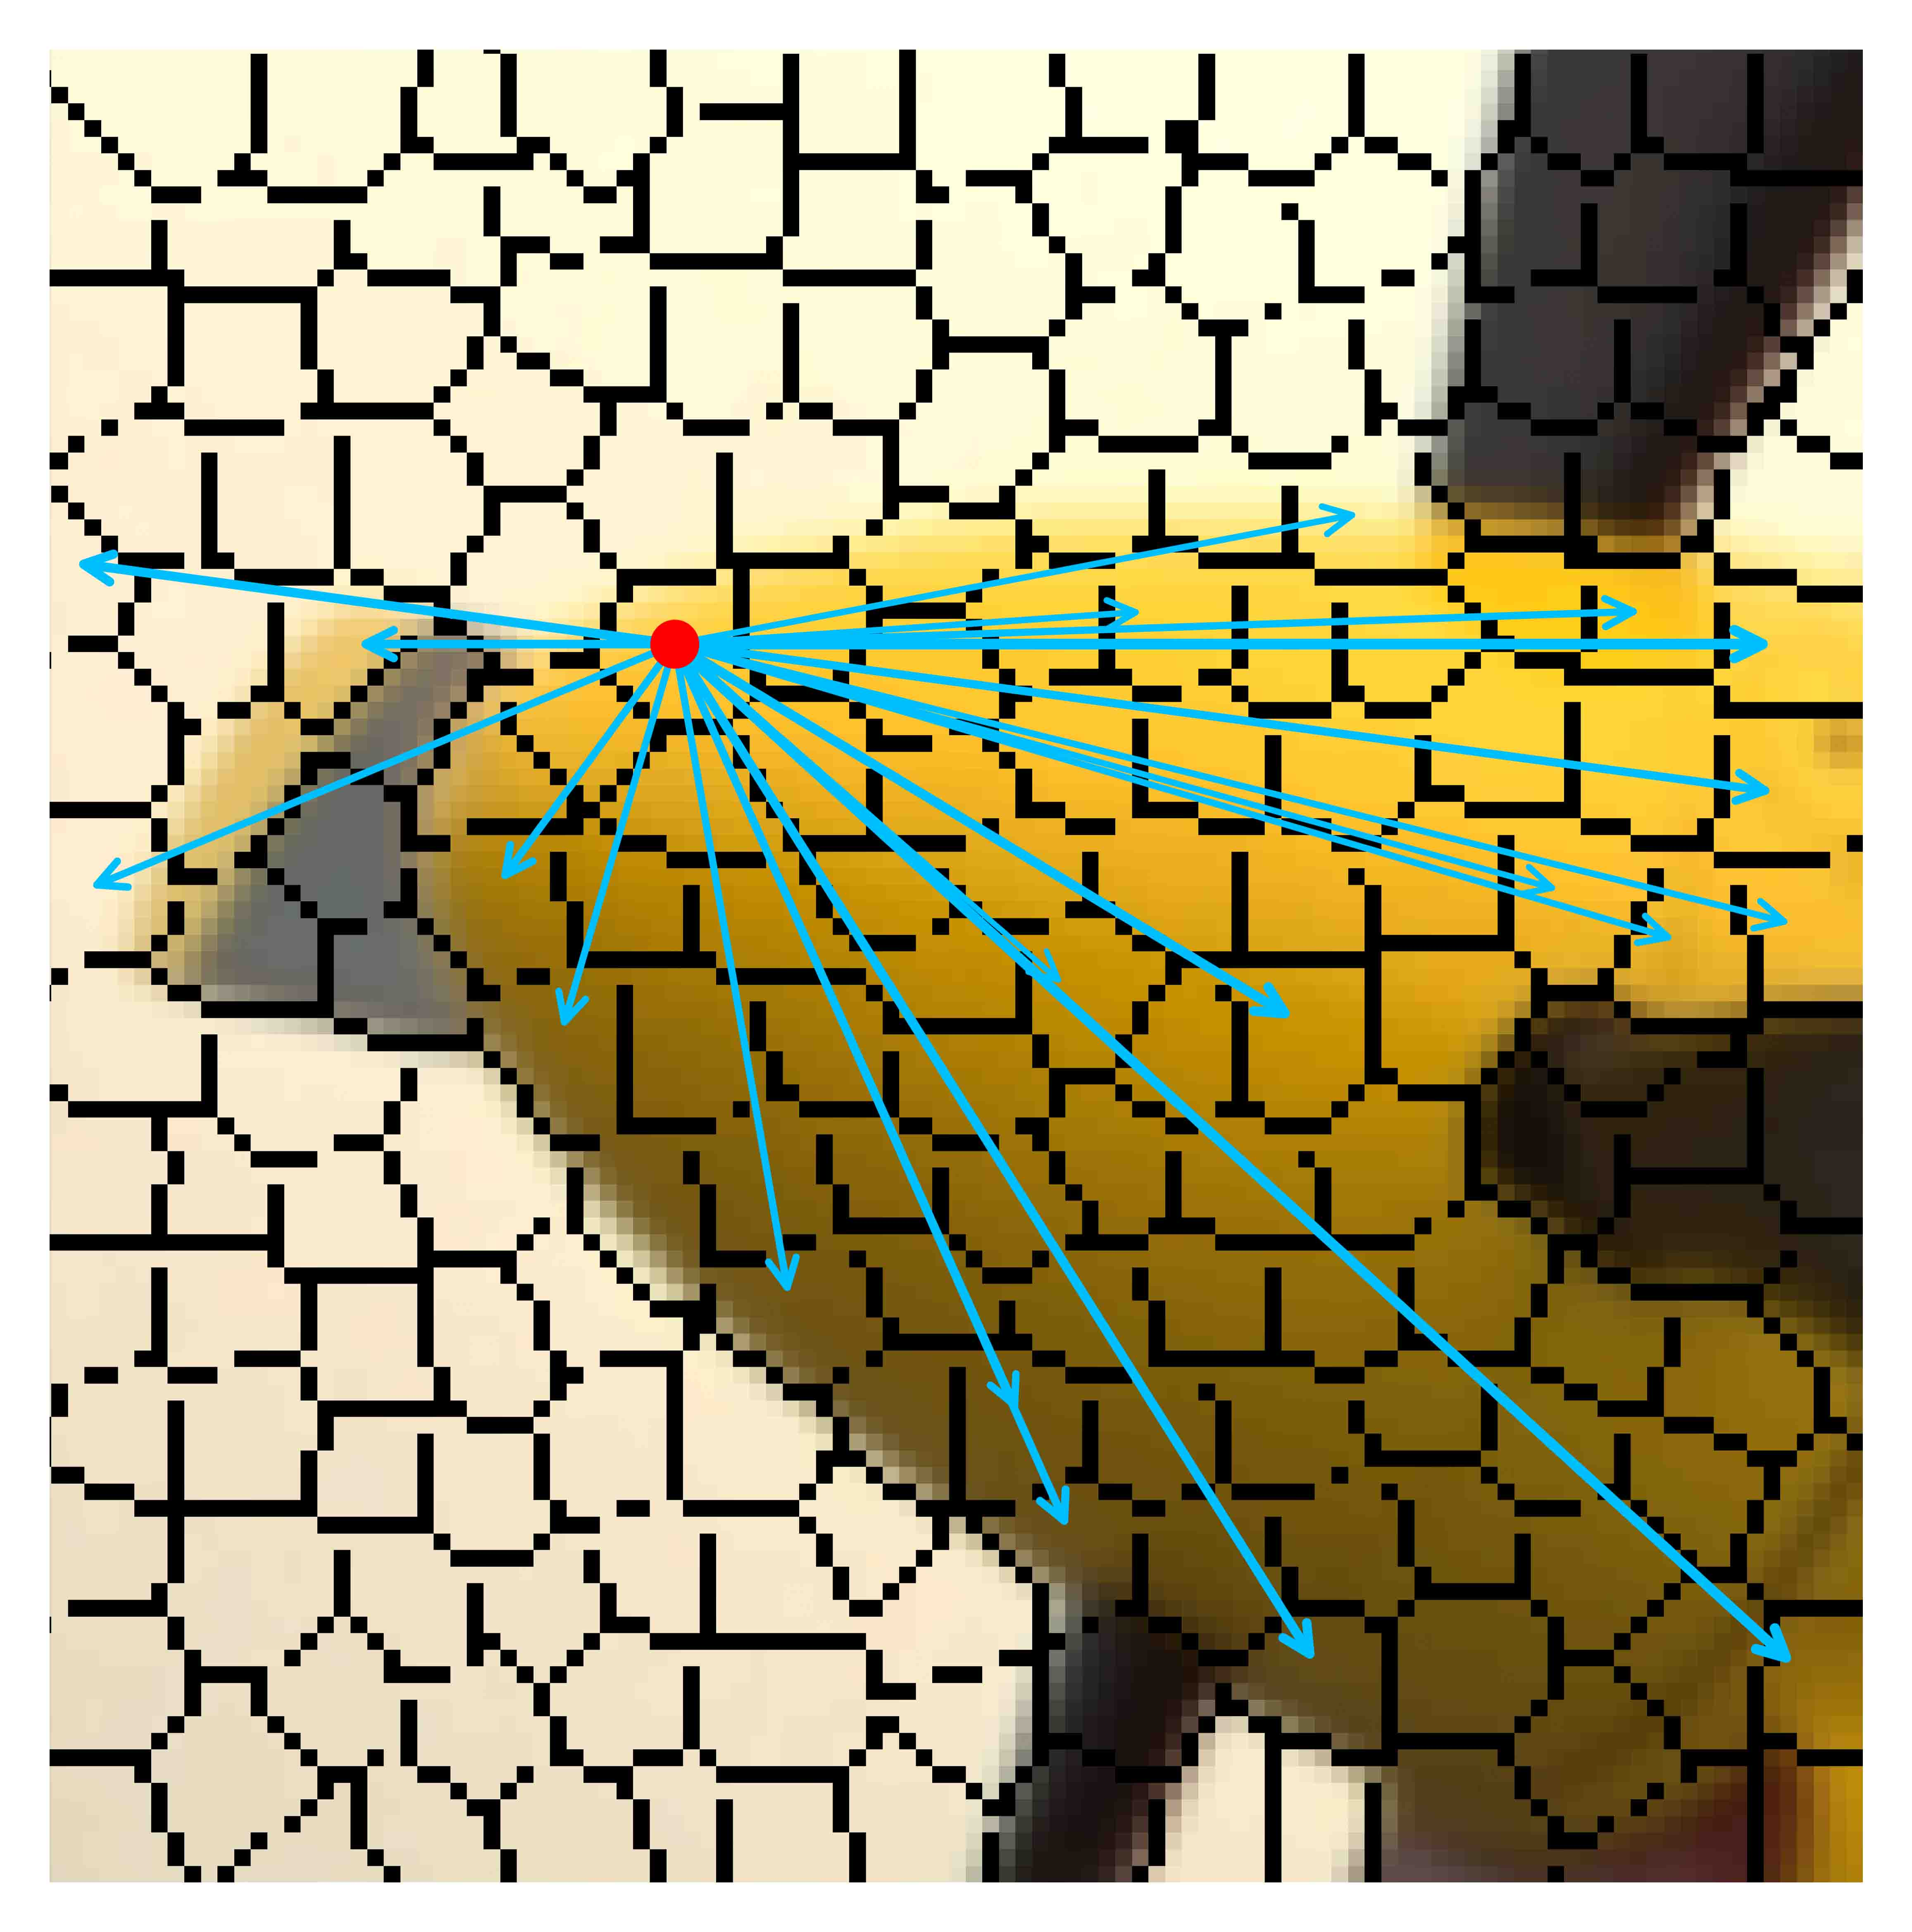
\includegraphics[width=1.5in]{cropped/jet_superpixel_4.jpg}
		\centerline{(a)}
	\end{minipage}
	\begin{minipage}[t]{.24\linewidth}
		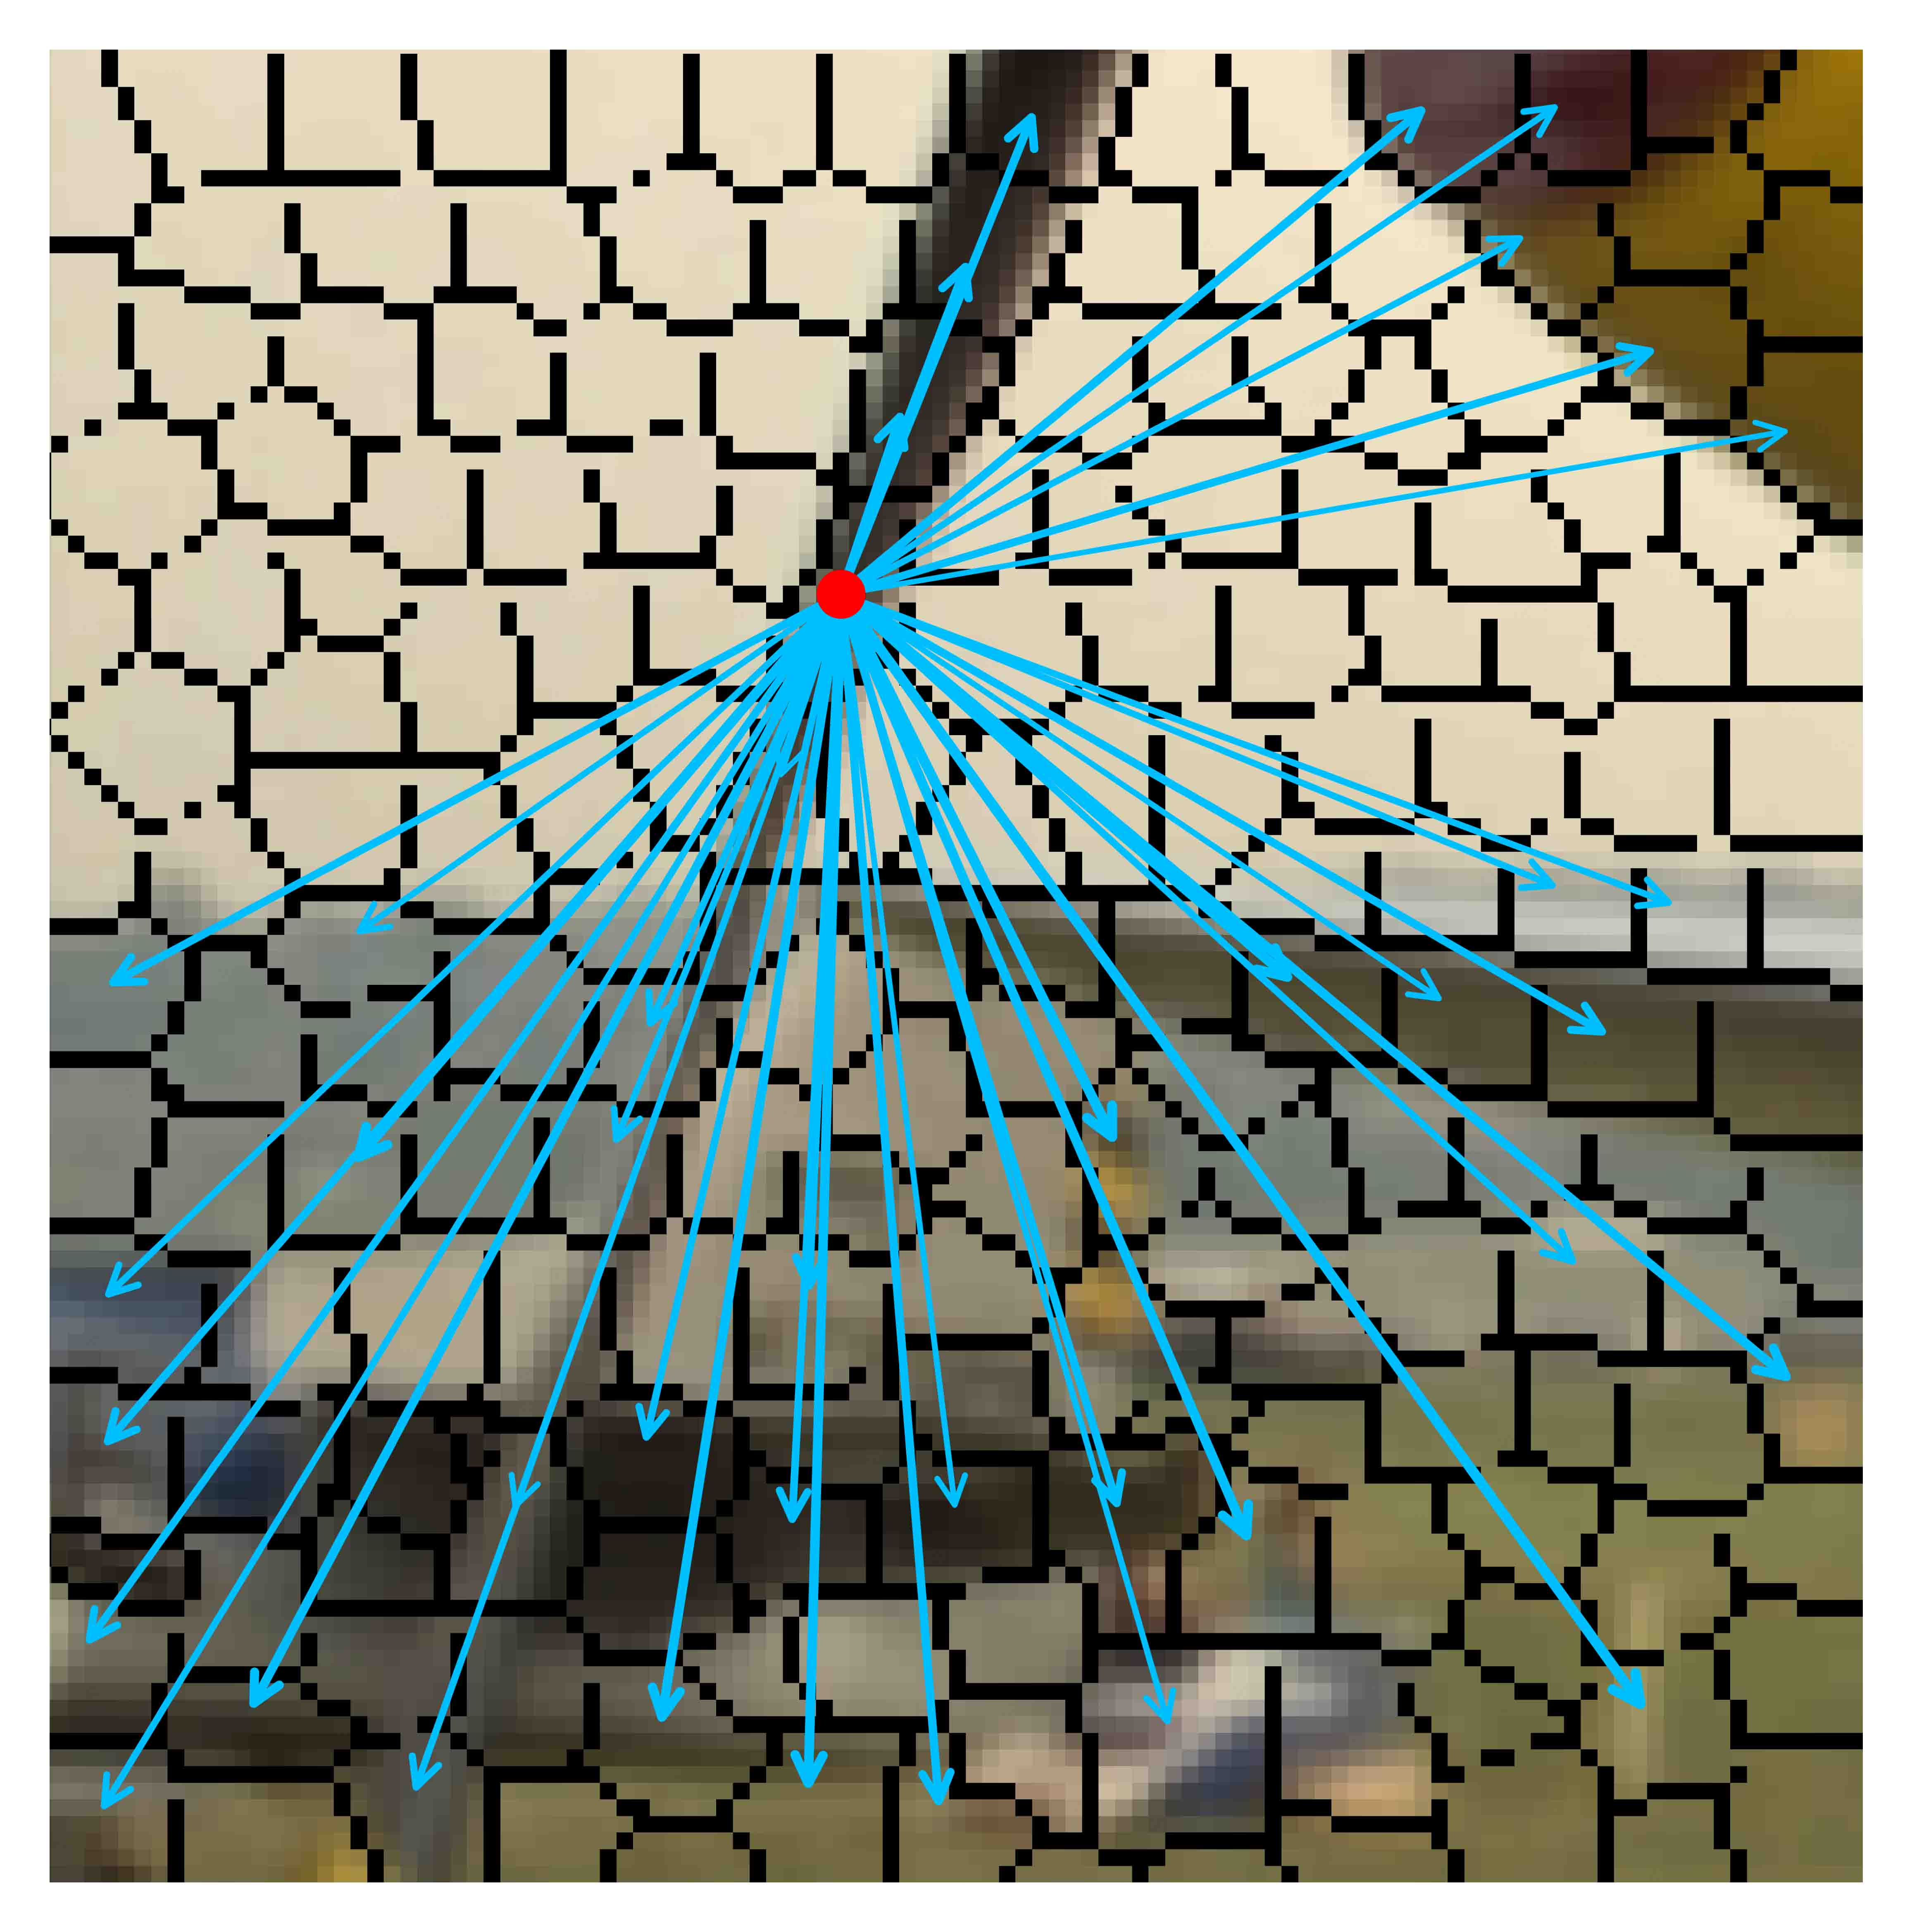
\includegraphics[width=1.5in]{cropped/jet_superpixel_8.jpg}
		\centerline{(b)}
	\end{minipage}
	\begin{minipage}[t]{.24\linewidth}
		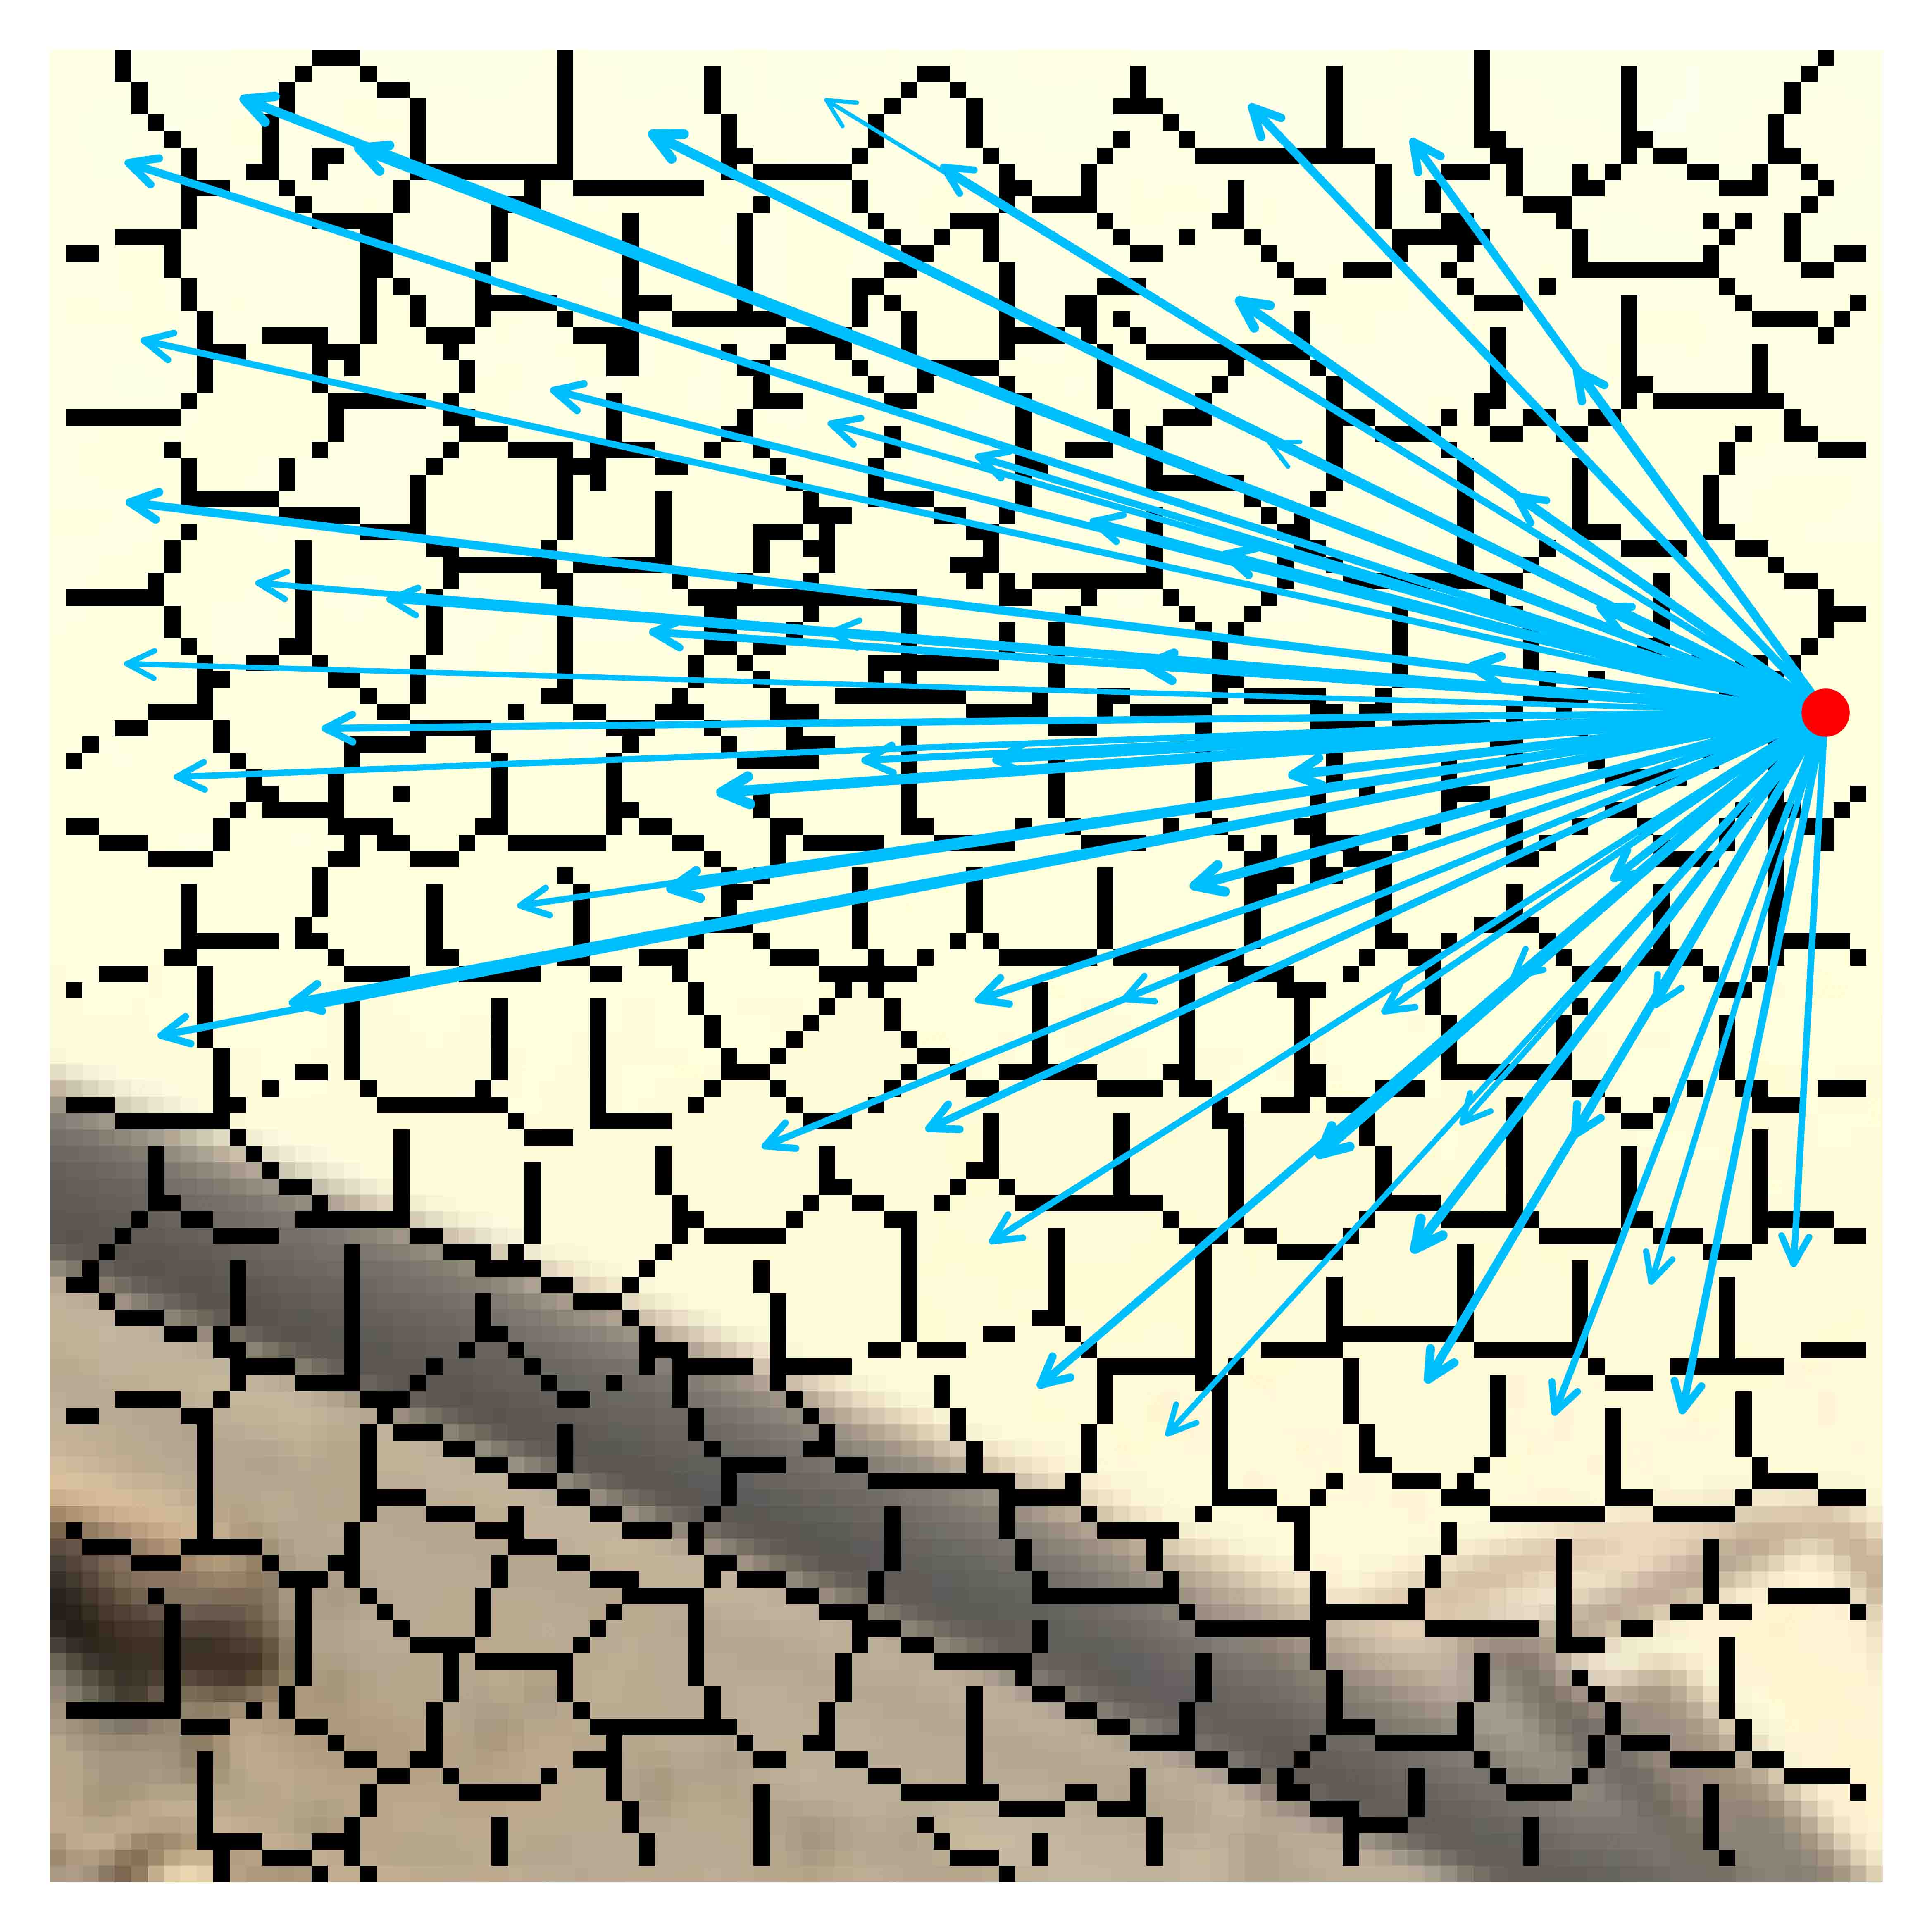
\includegraphics[width=1.5in]{cropped/jet_superpixel_6.jpg}
		\centerline{(c)}
	\end{minipage}
	\begin{minipage}[t]{.24\linewidth}
		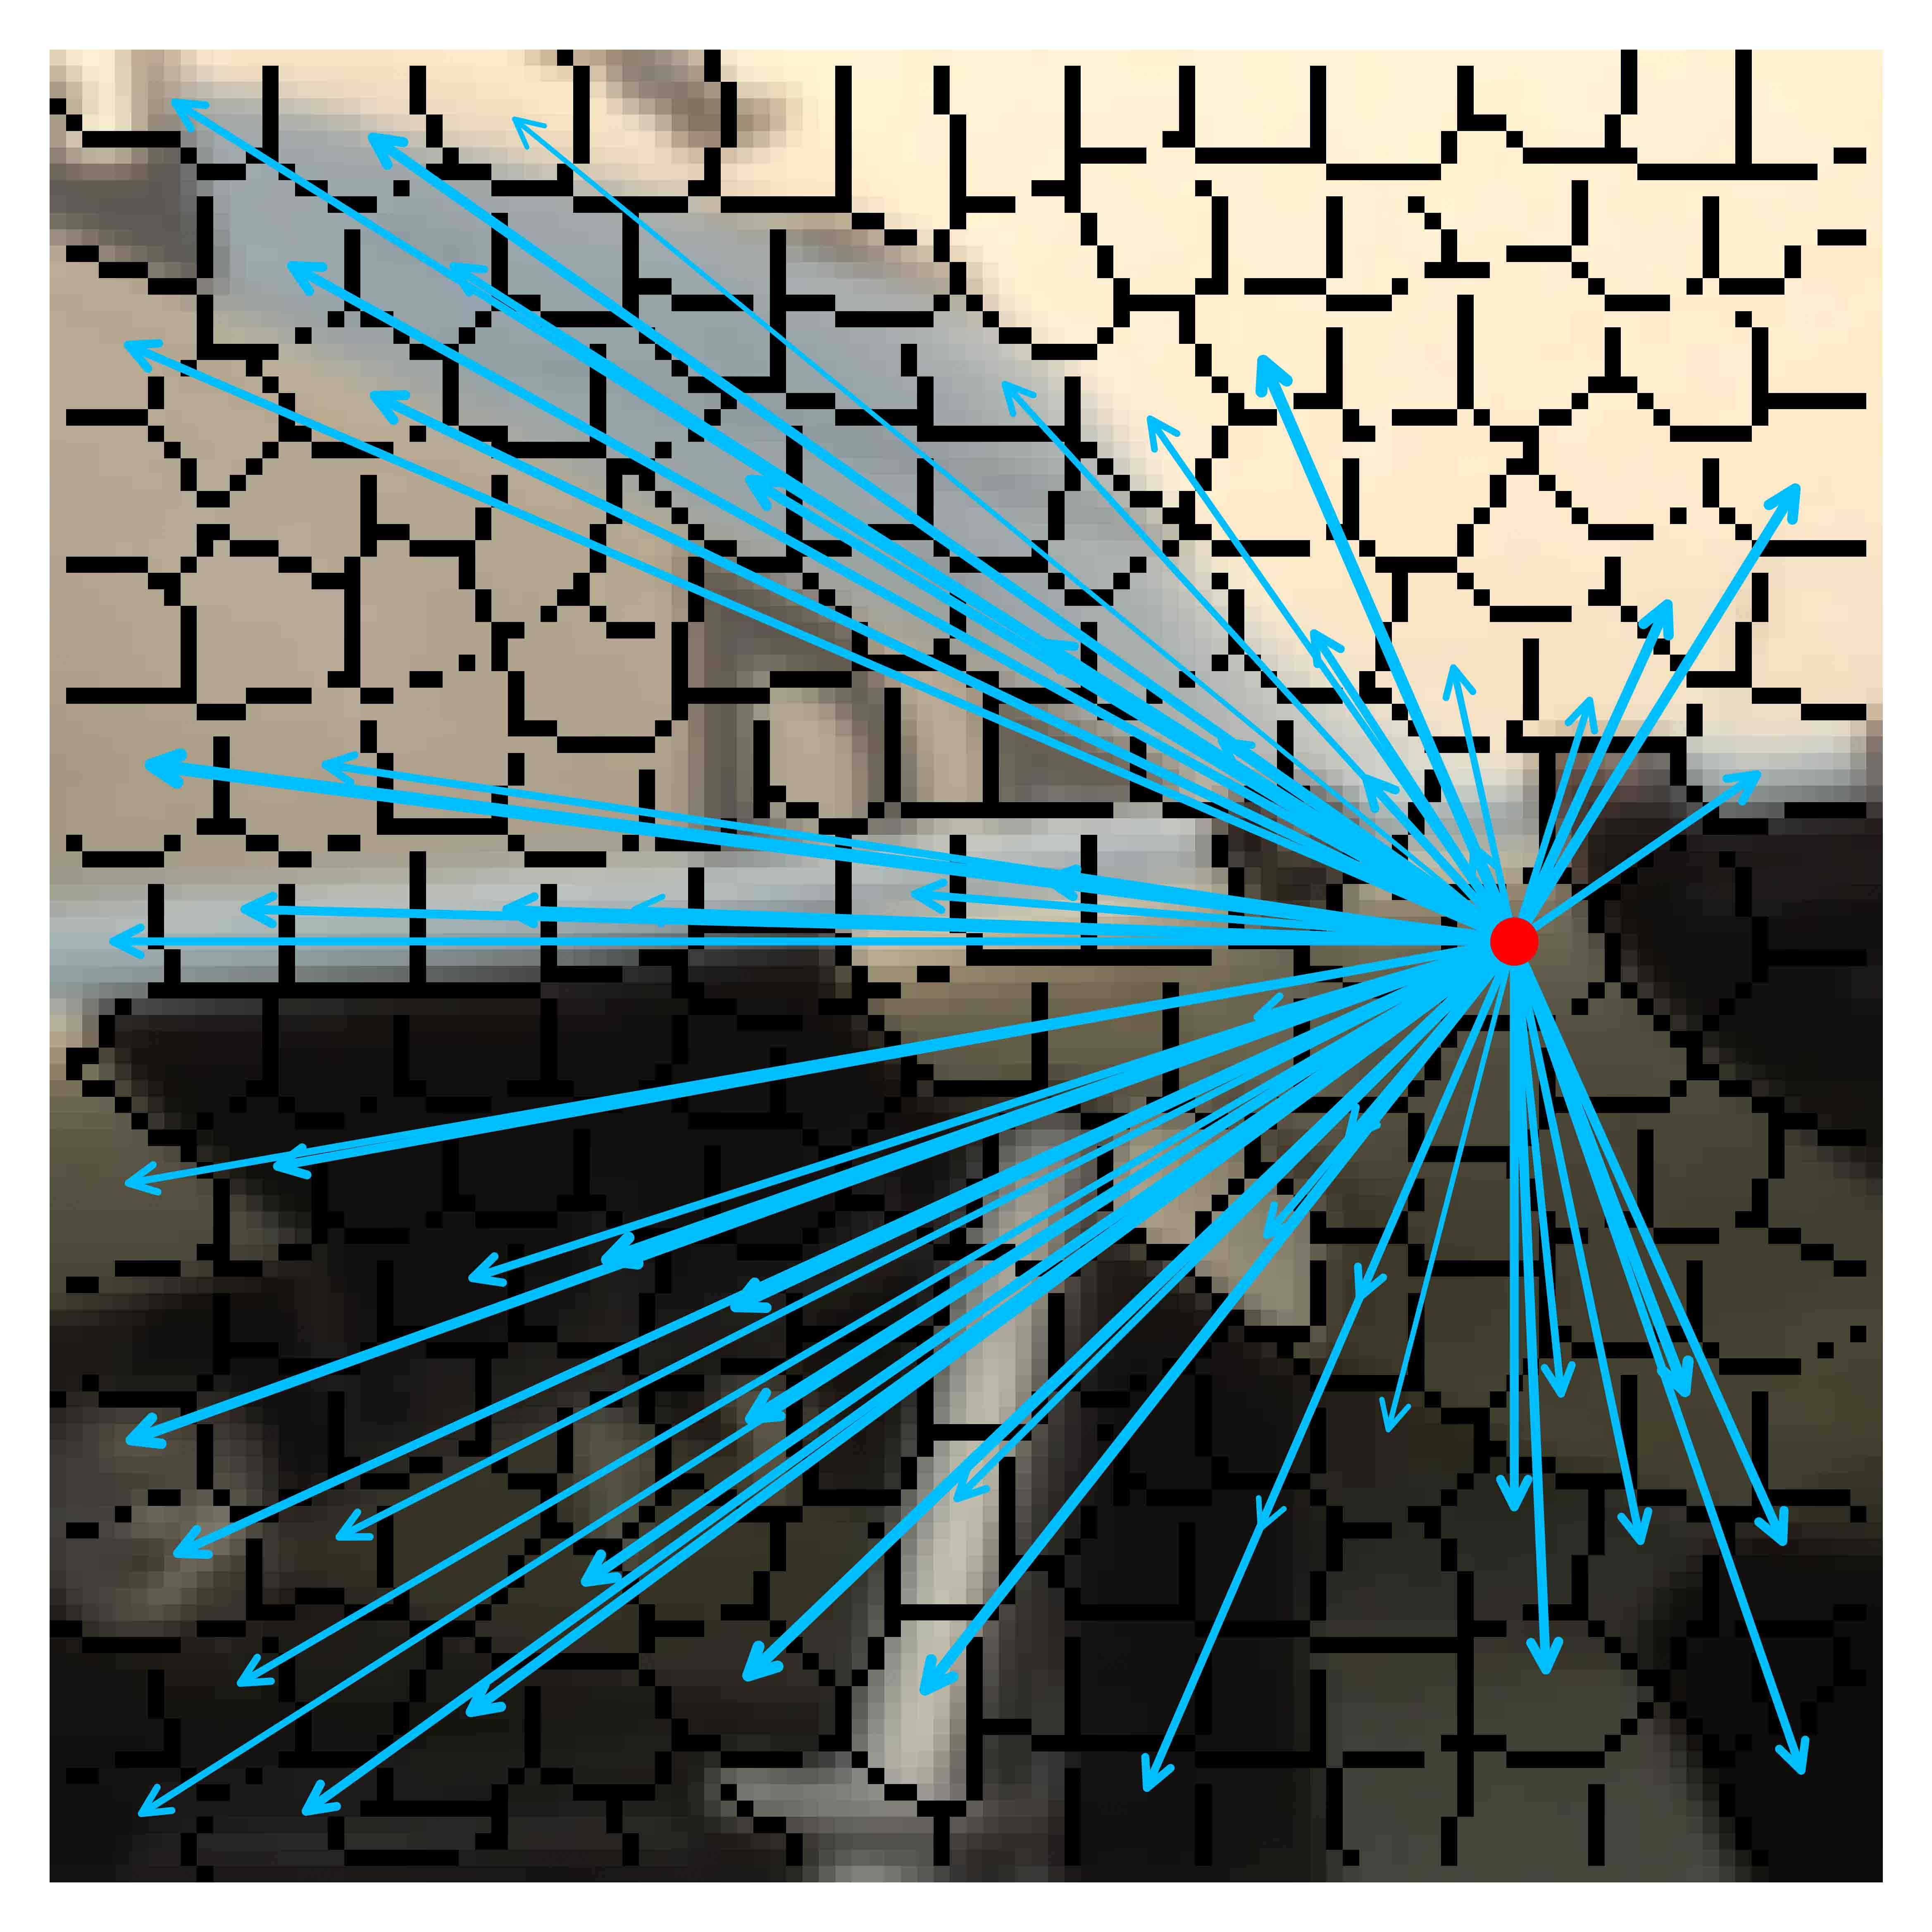
\includegraphics[width=1.5in]{cropped/jet_superpixel_11.jpg}
		\centerline{(d)}
	\end{minipage}
	\begin{minipage}[t]{.24\linewidth}
		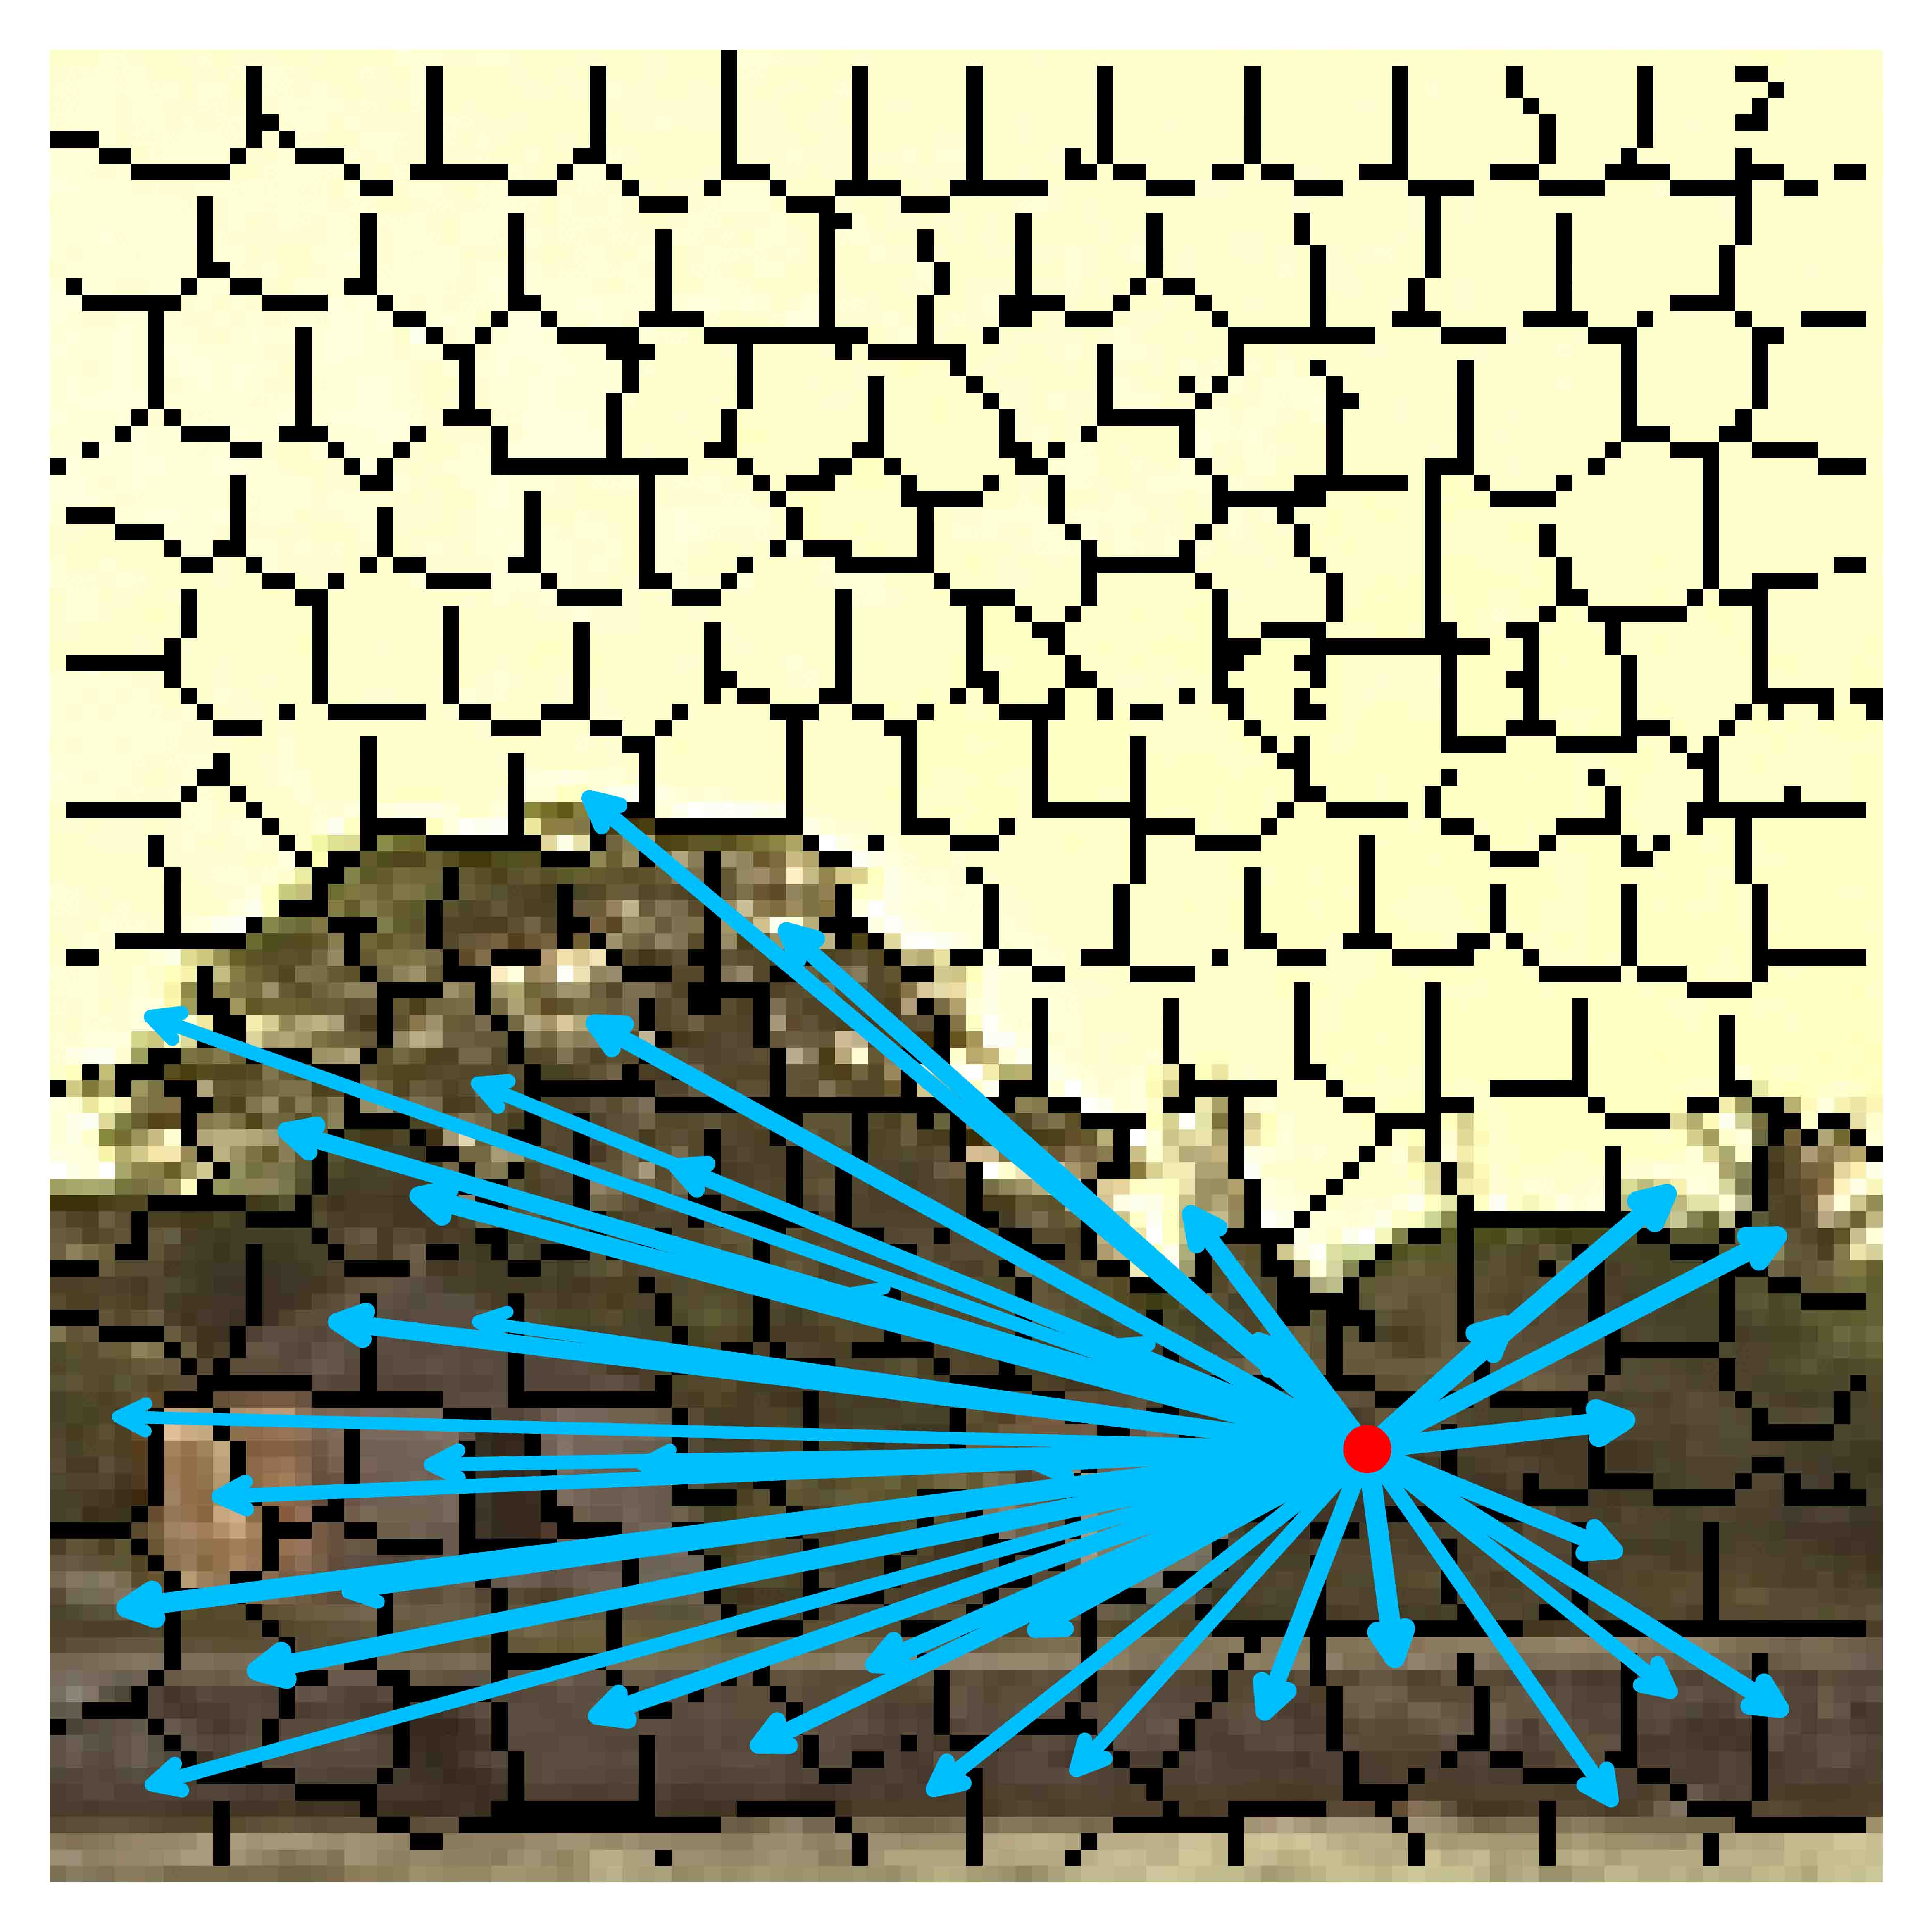
\includegraphics[width=1.5in]{cropped/boat_superpixel_0.jpg}
		\centerline{(e)}
	\end{minipage}
	\begin{minipage}[t]{.24\linewidth}
		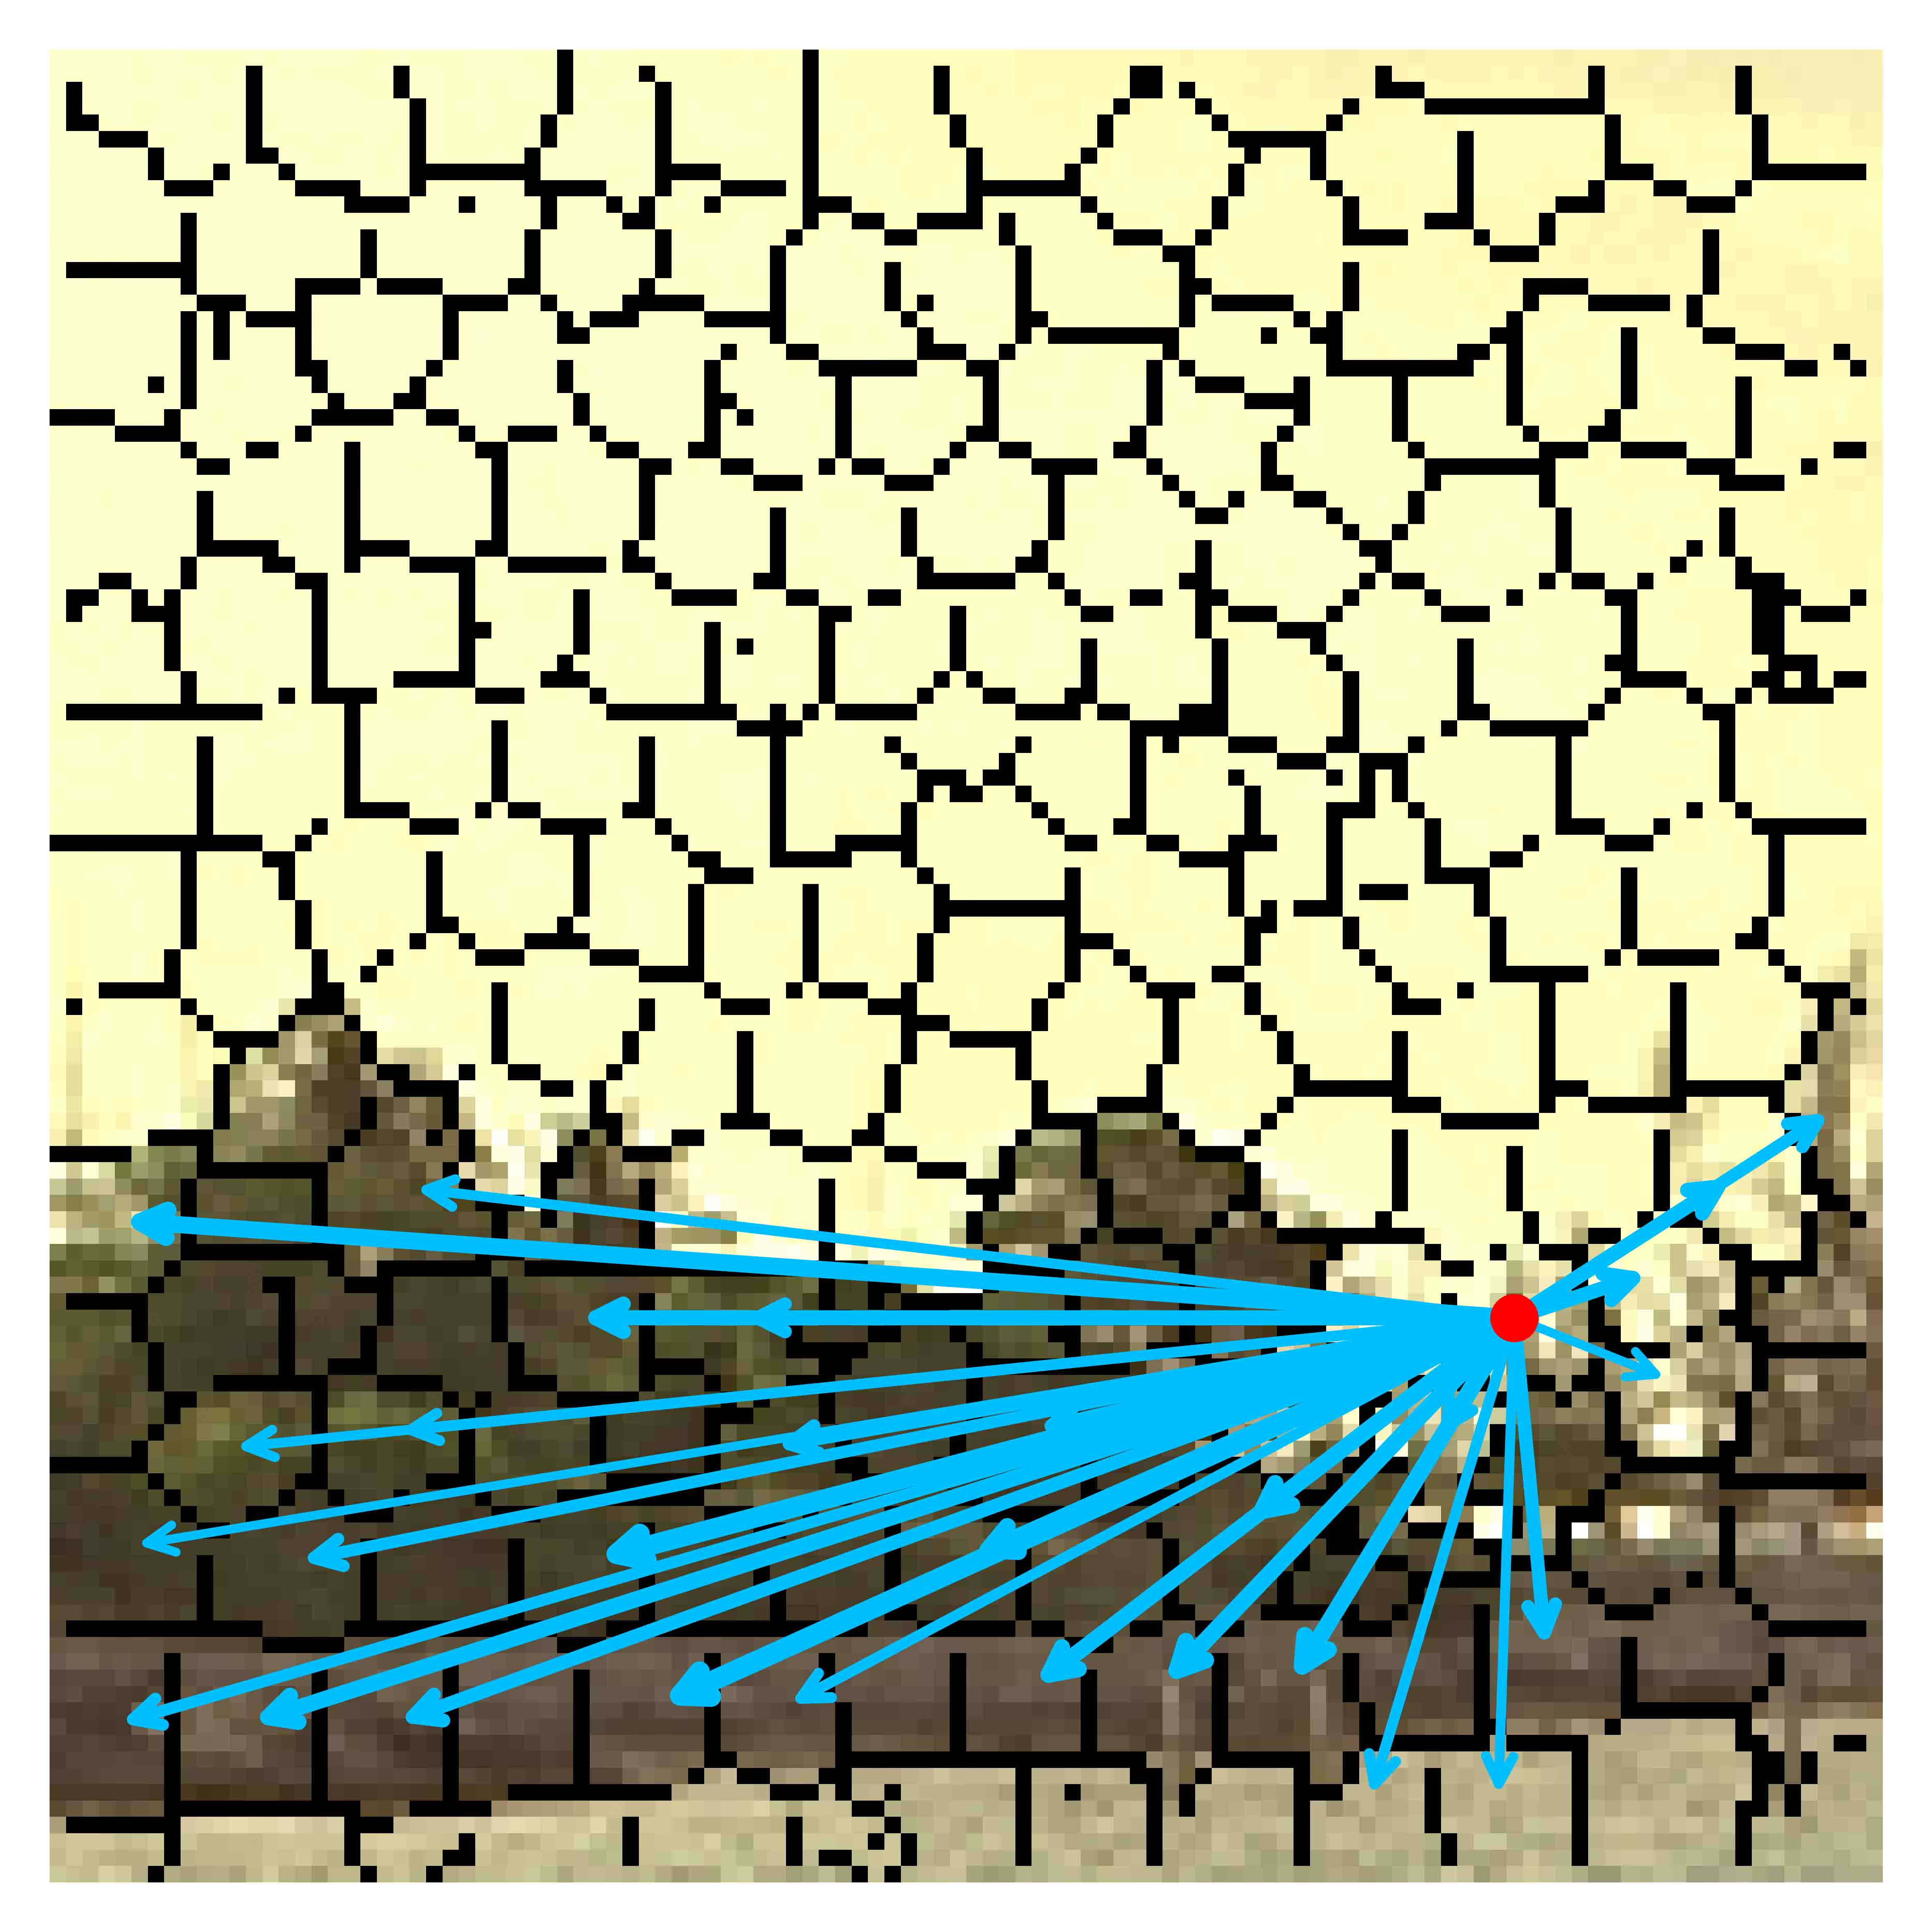
\includegraphics[width=1.5in]{cropped/boat_superpixel_1.jpg}
		\centerline{(f)}
	\end{minipage}
	\begin{minipage}[t]{.24\linewidth}
		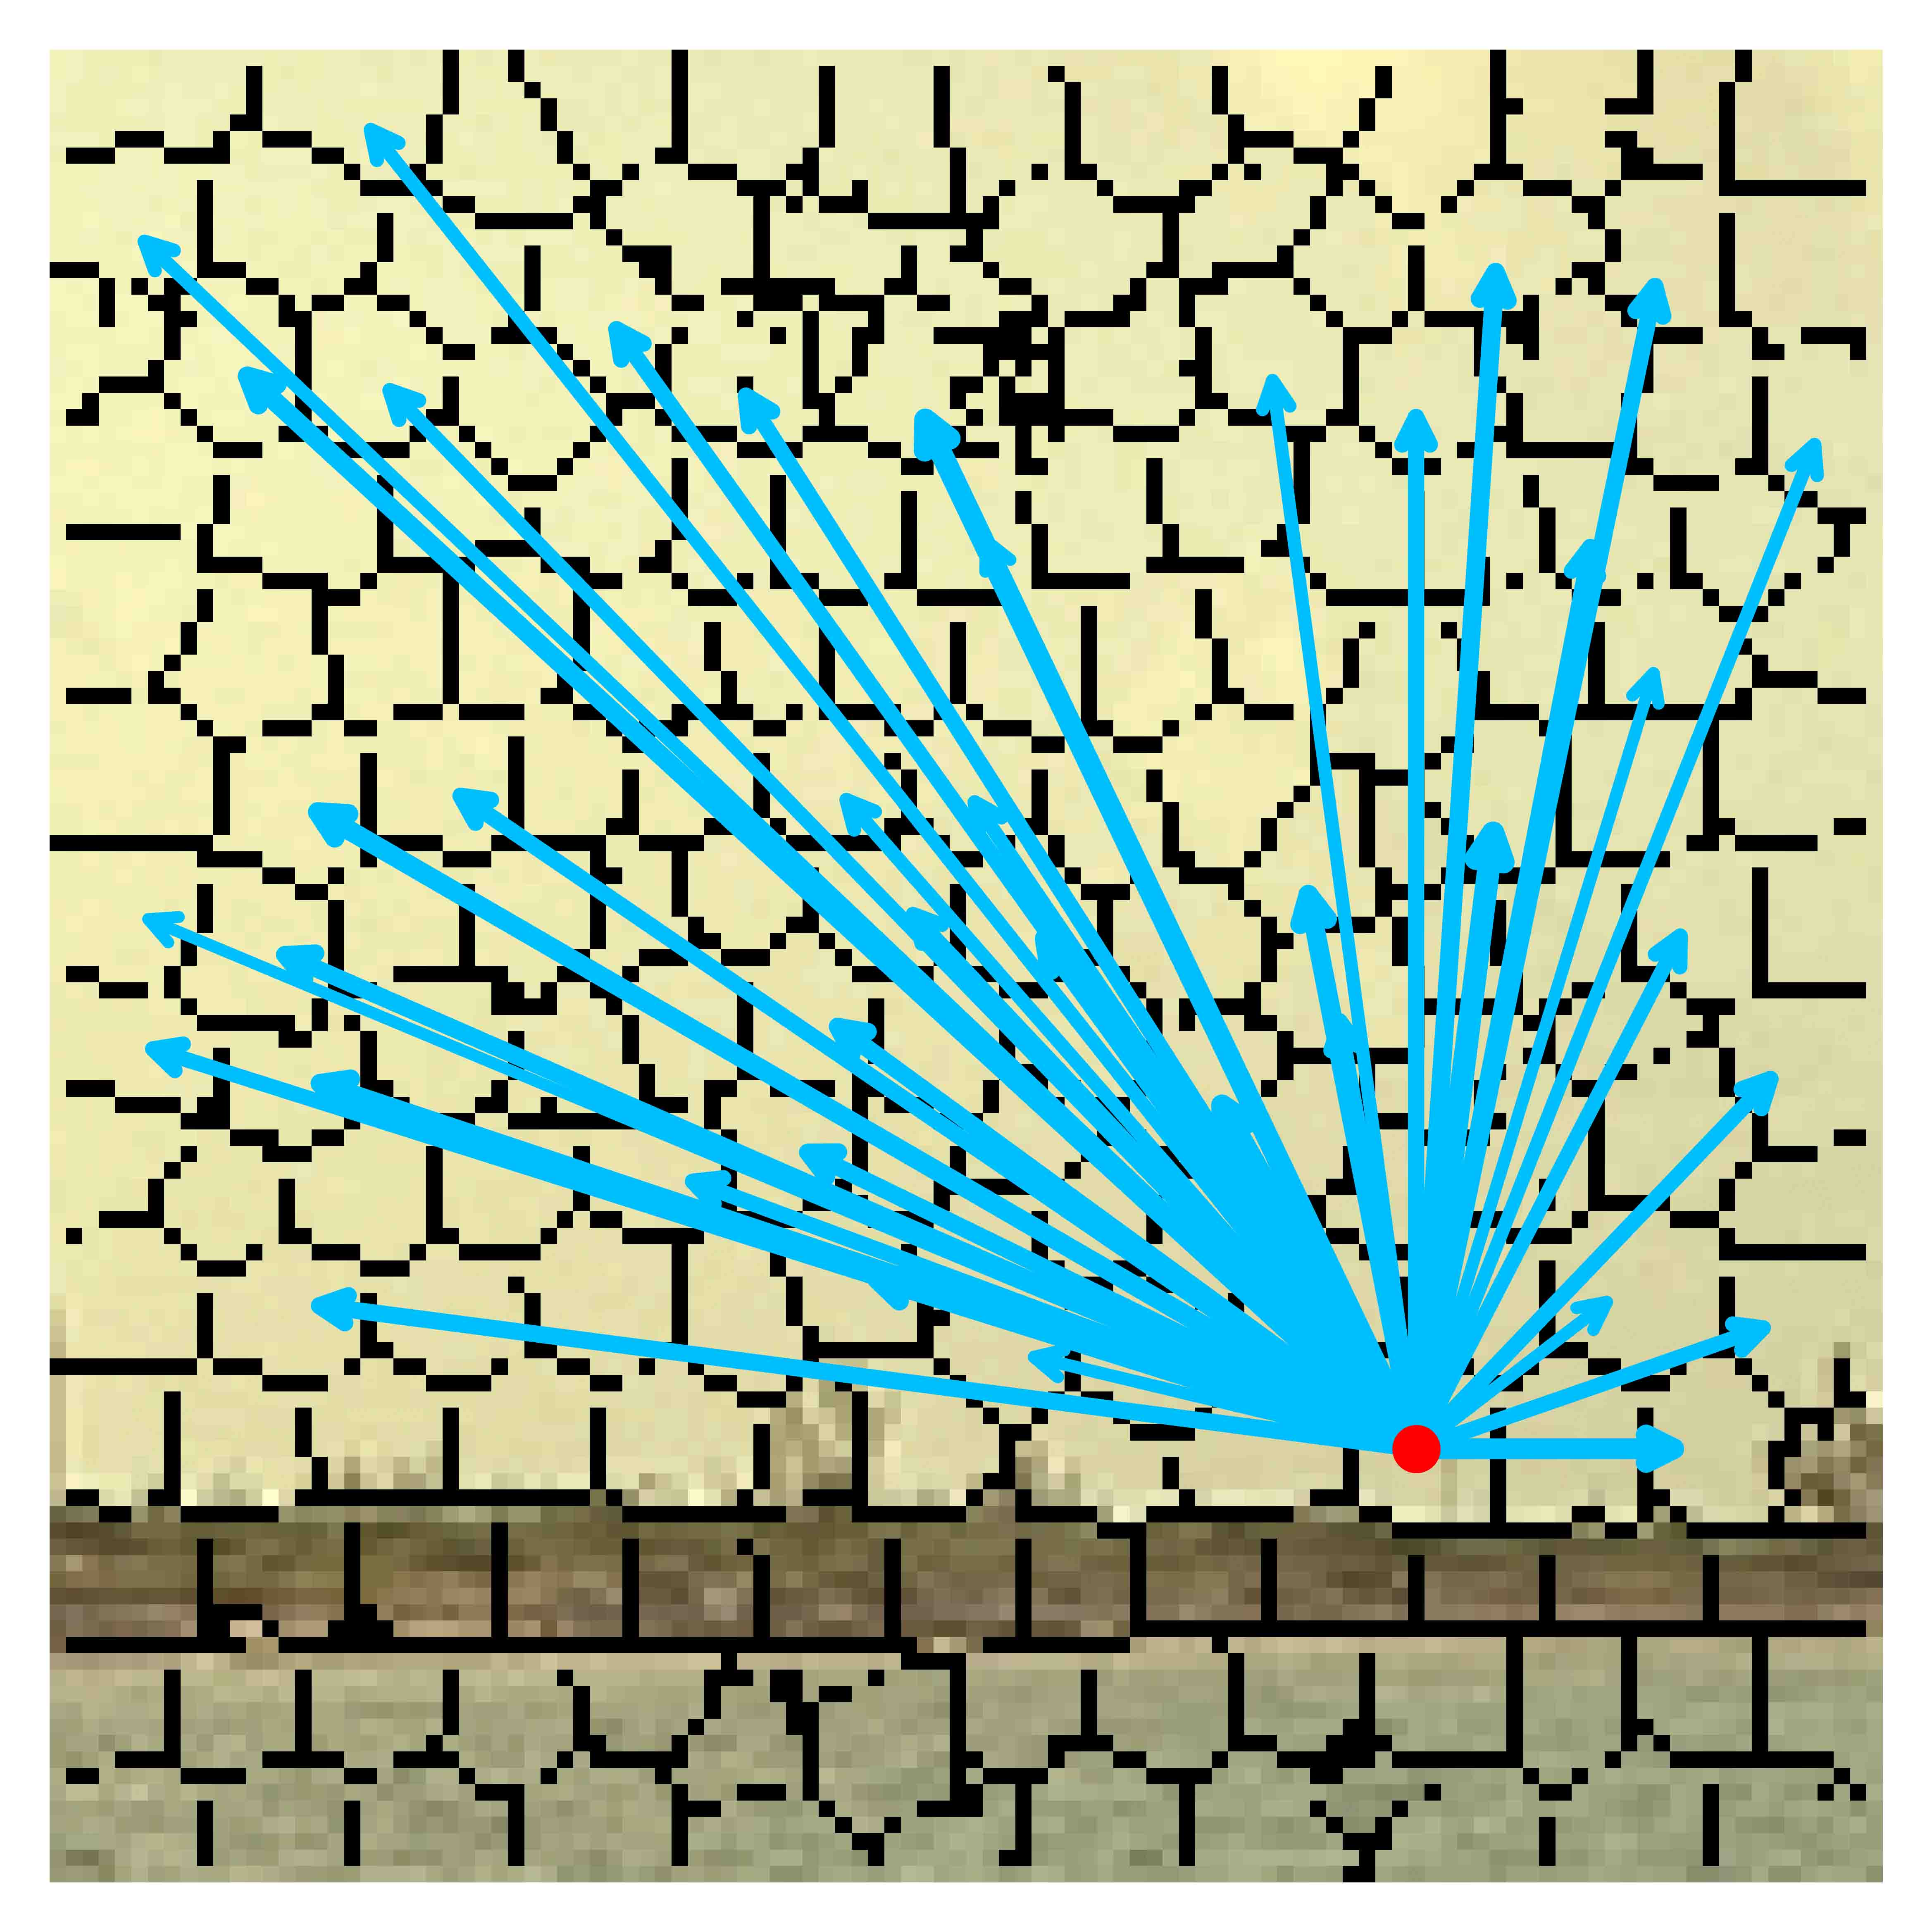
\includegraphics[width=1.5in]{cropped/boat_superpixel_3.jpg}
		\centerline{(g)}
	\end{minipage}
	\begin{minipage}[t]{.24\linewidth}
		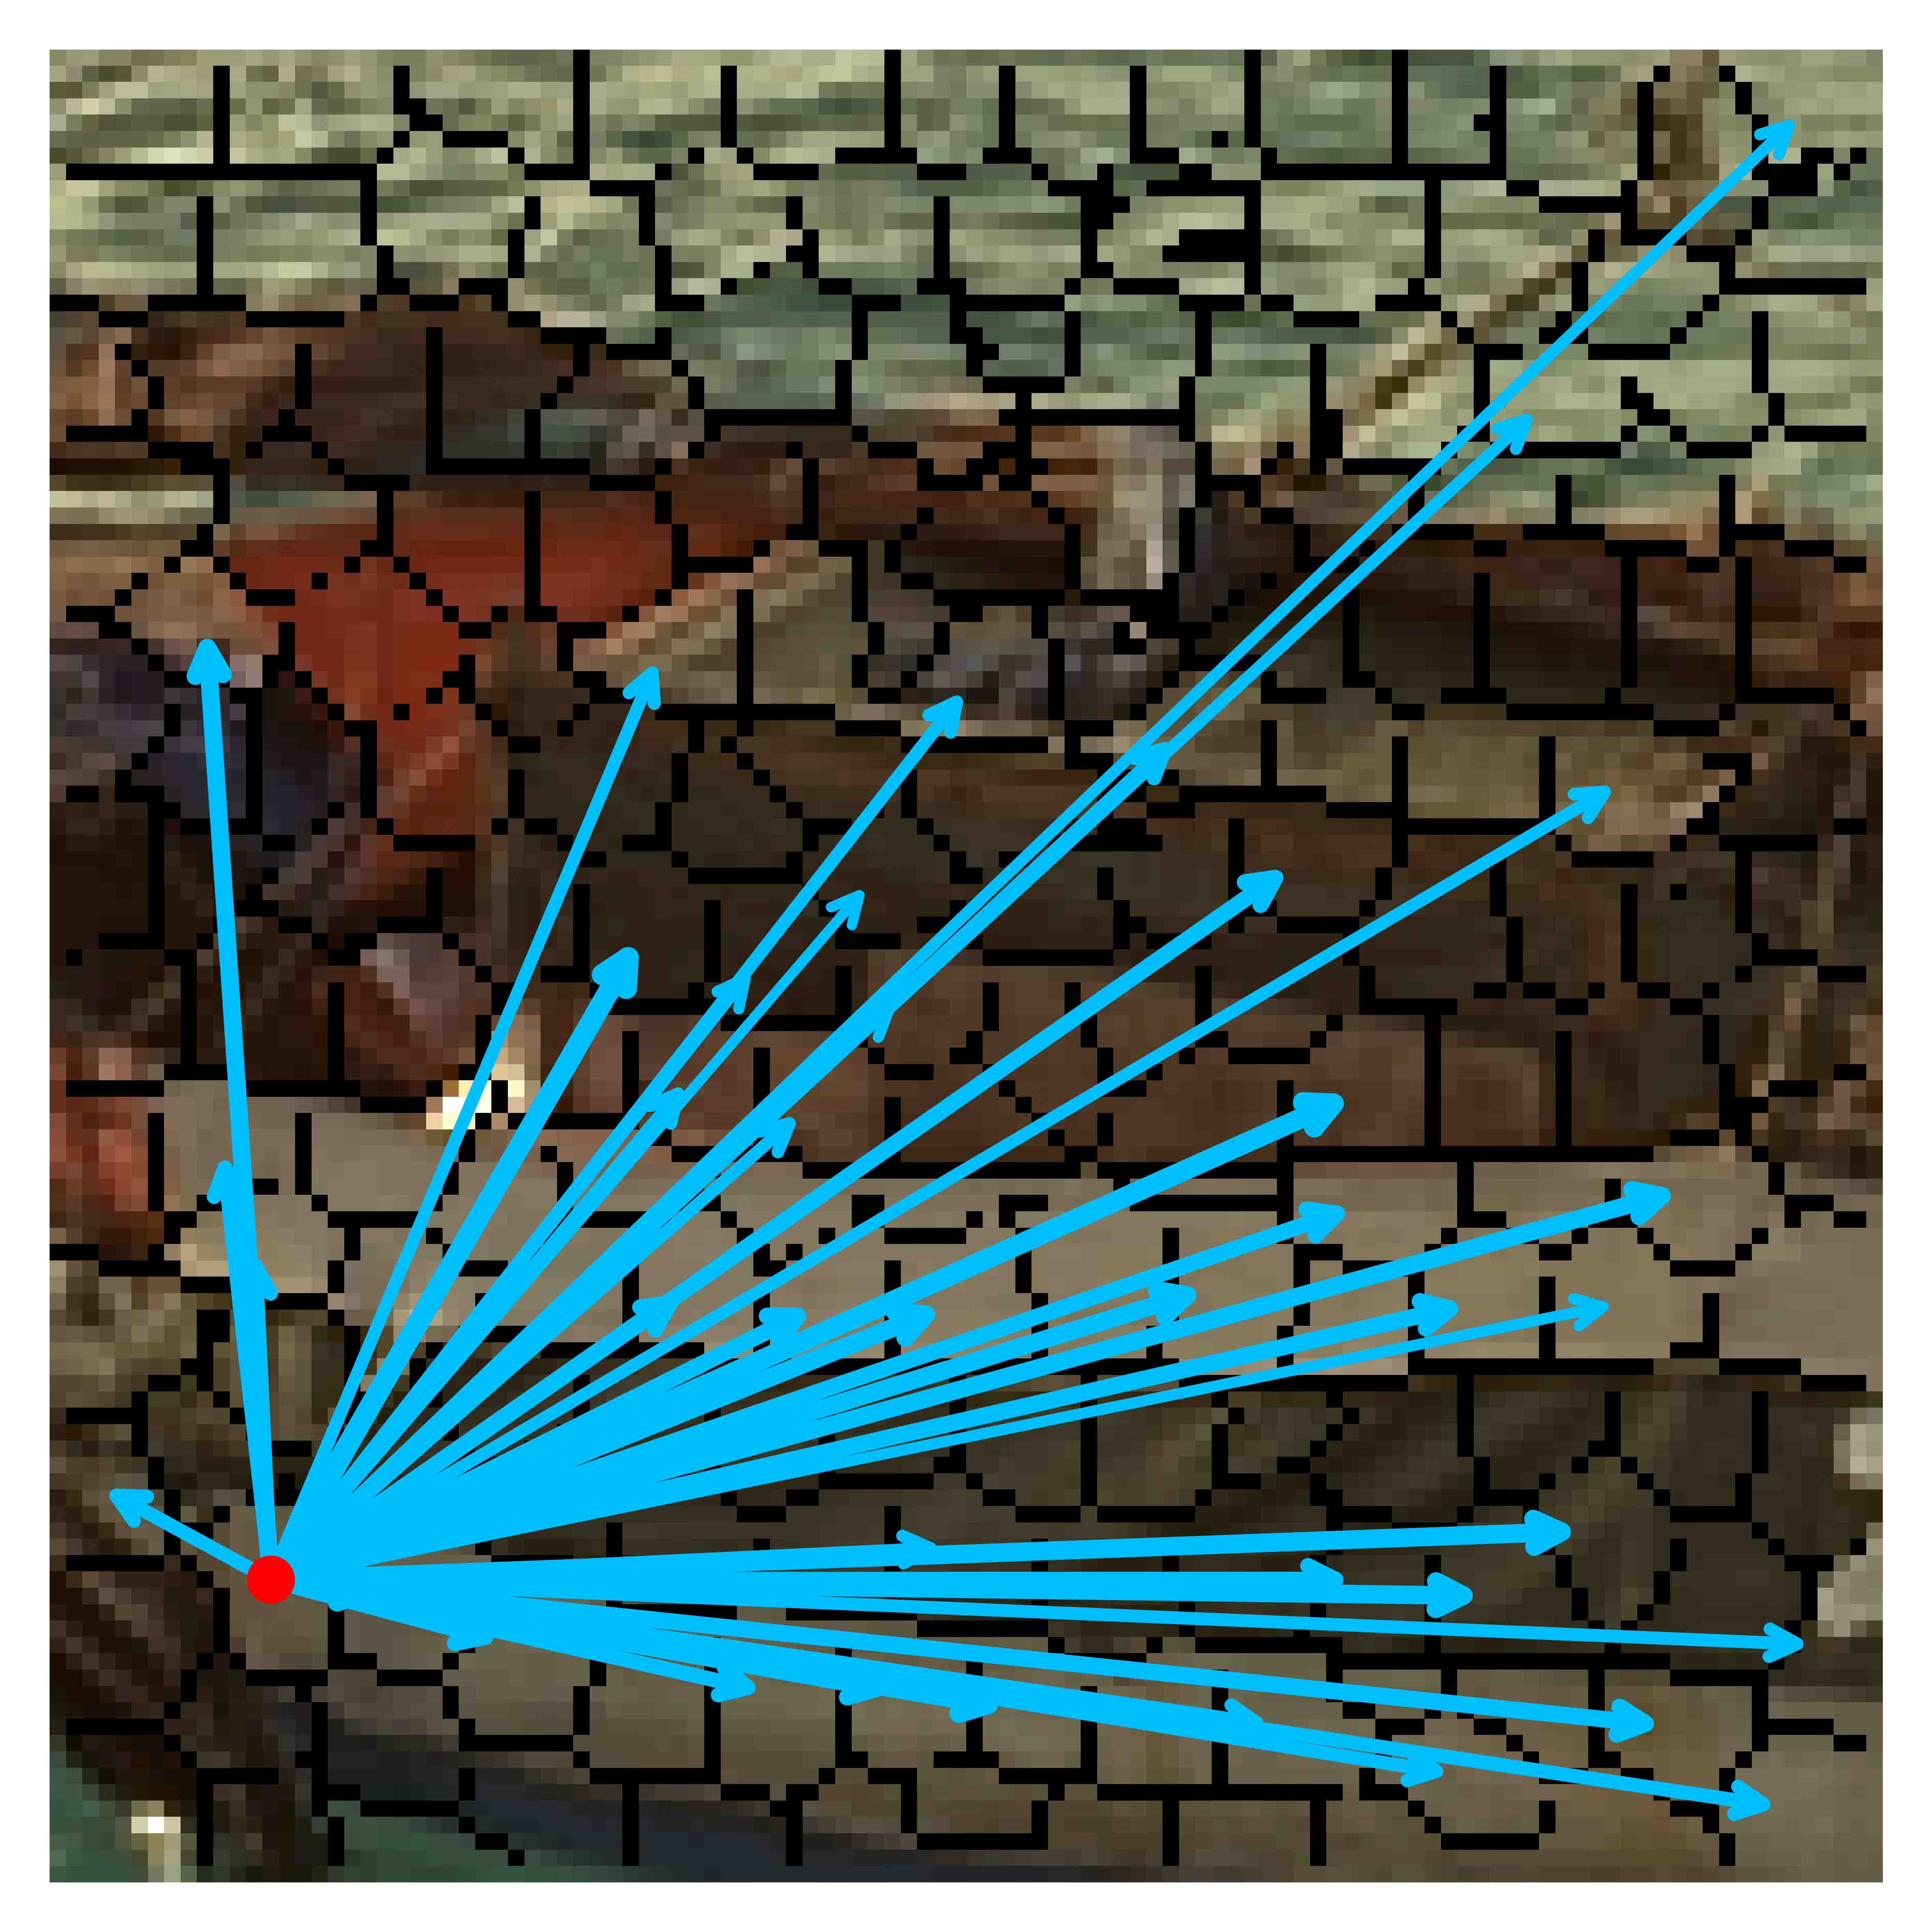
\includegraphics[width=1.5in]{cropped/boat_superpixel_9.jpg}
		\centerline{(h)}
	\end{minipage}
	\begin{minipage}[t]{.24\linewidth}
		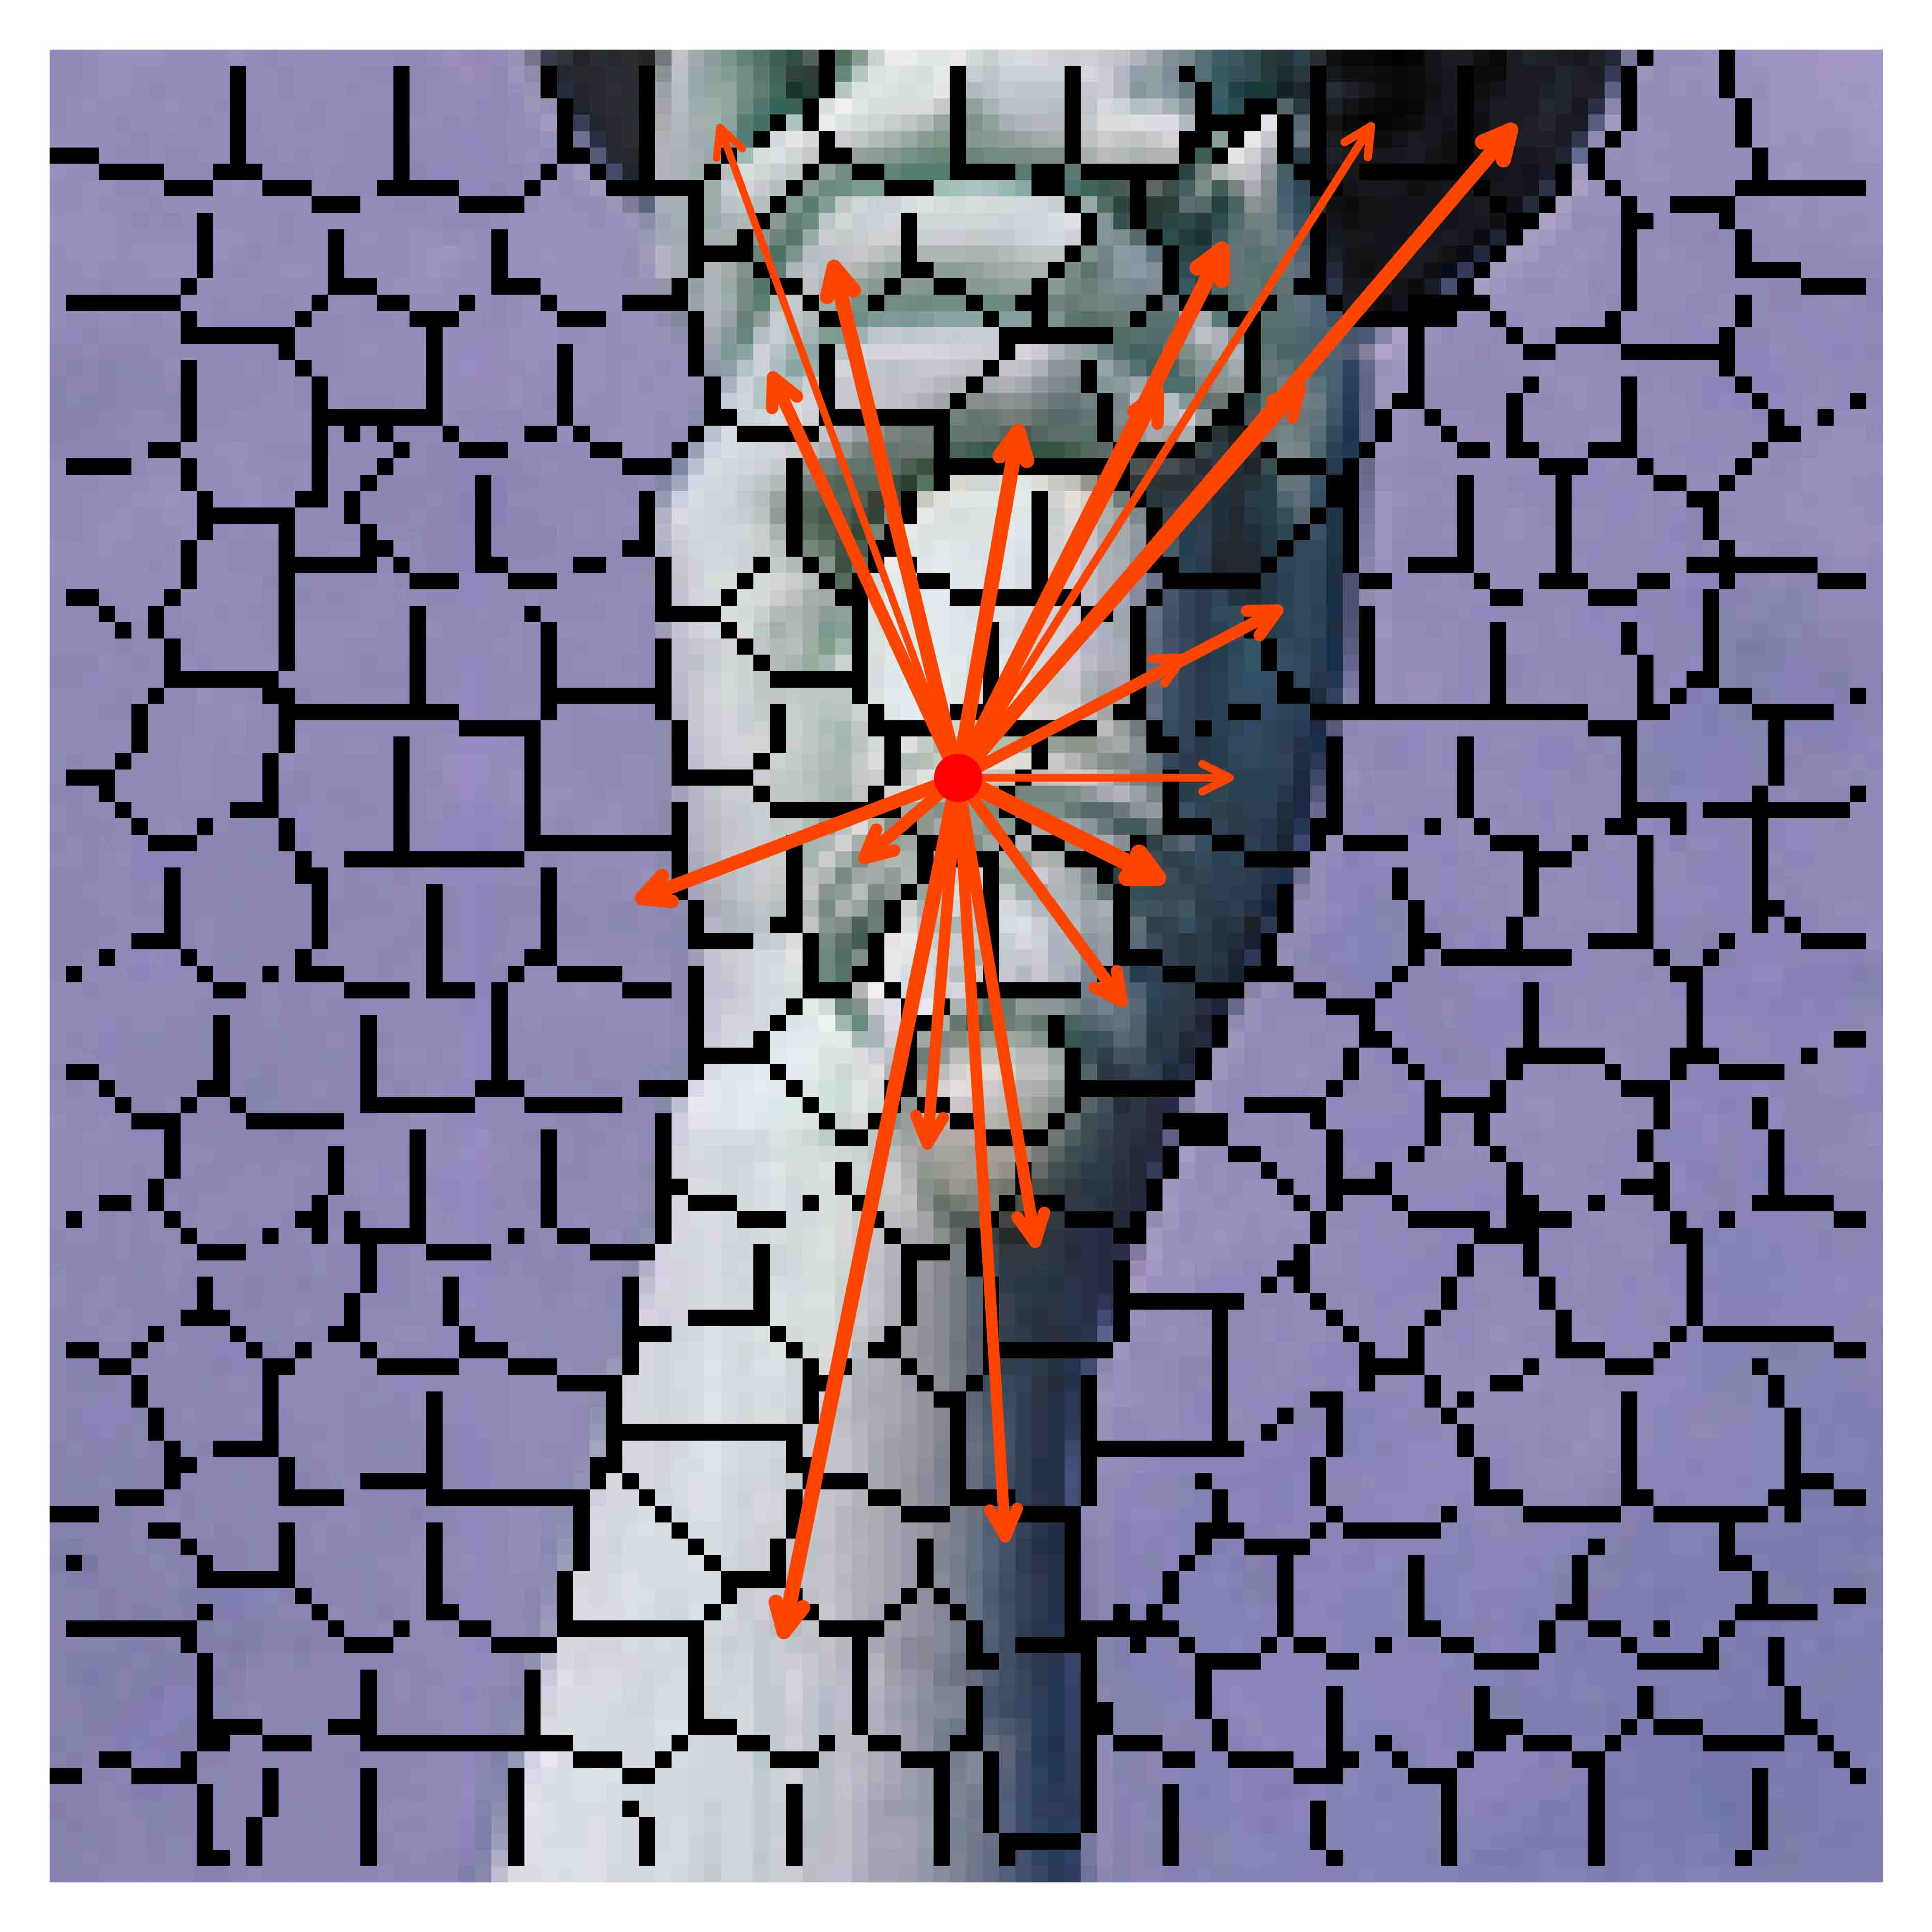
\includegraphics[width=1.5in]{cropped/lady_superpixel_1.jpg}
		\centerline{(i)}
	\end{minipage}
	\begin{minipage}[t]{.24\linewidth}
		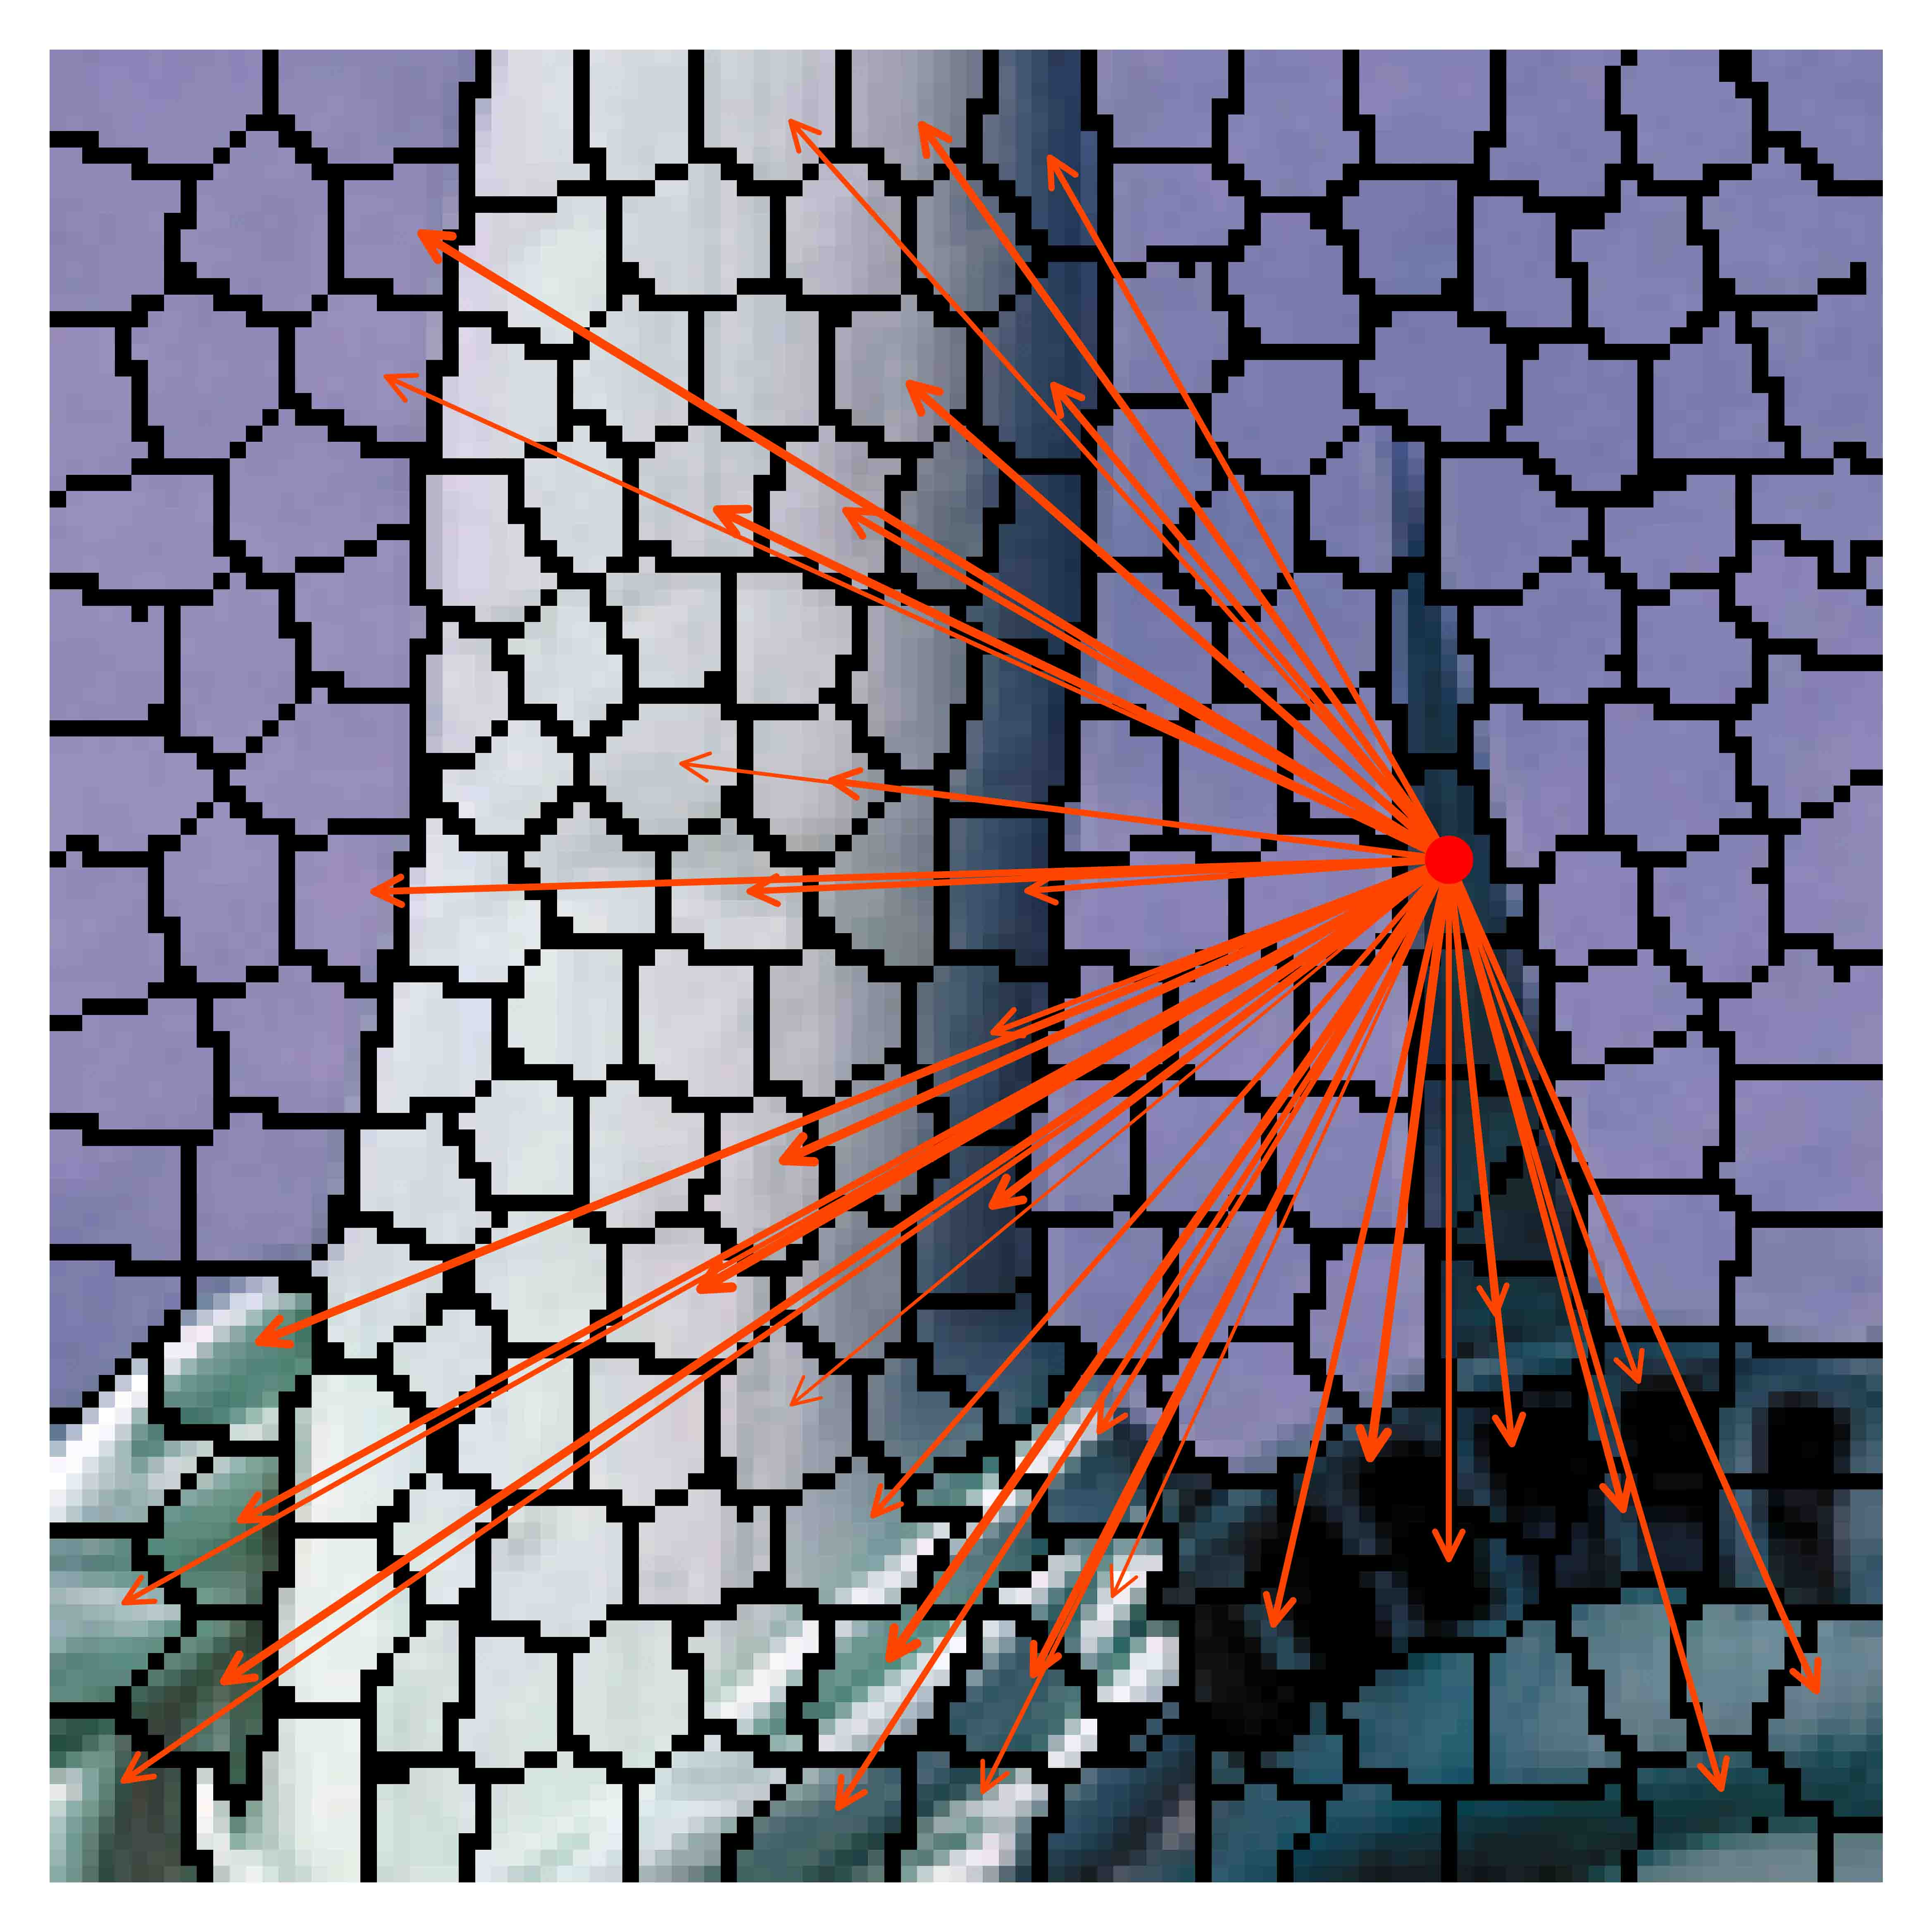
\includegraphics[width=1.5in]{cropped/lady_superpixel_5.jpg}
		\centerline{(j)}
	\end{minipage}
	\begin{minipage}[t]{.24\linewidth}
		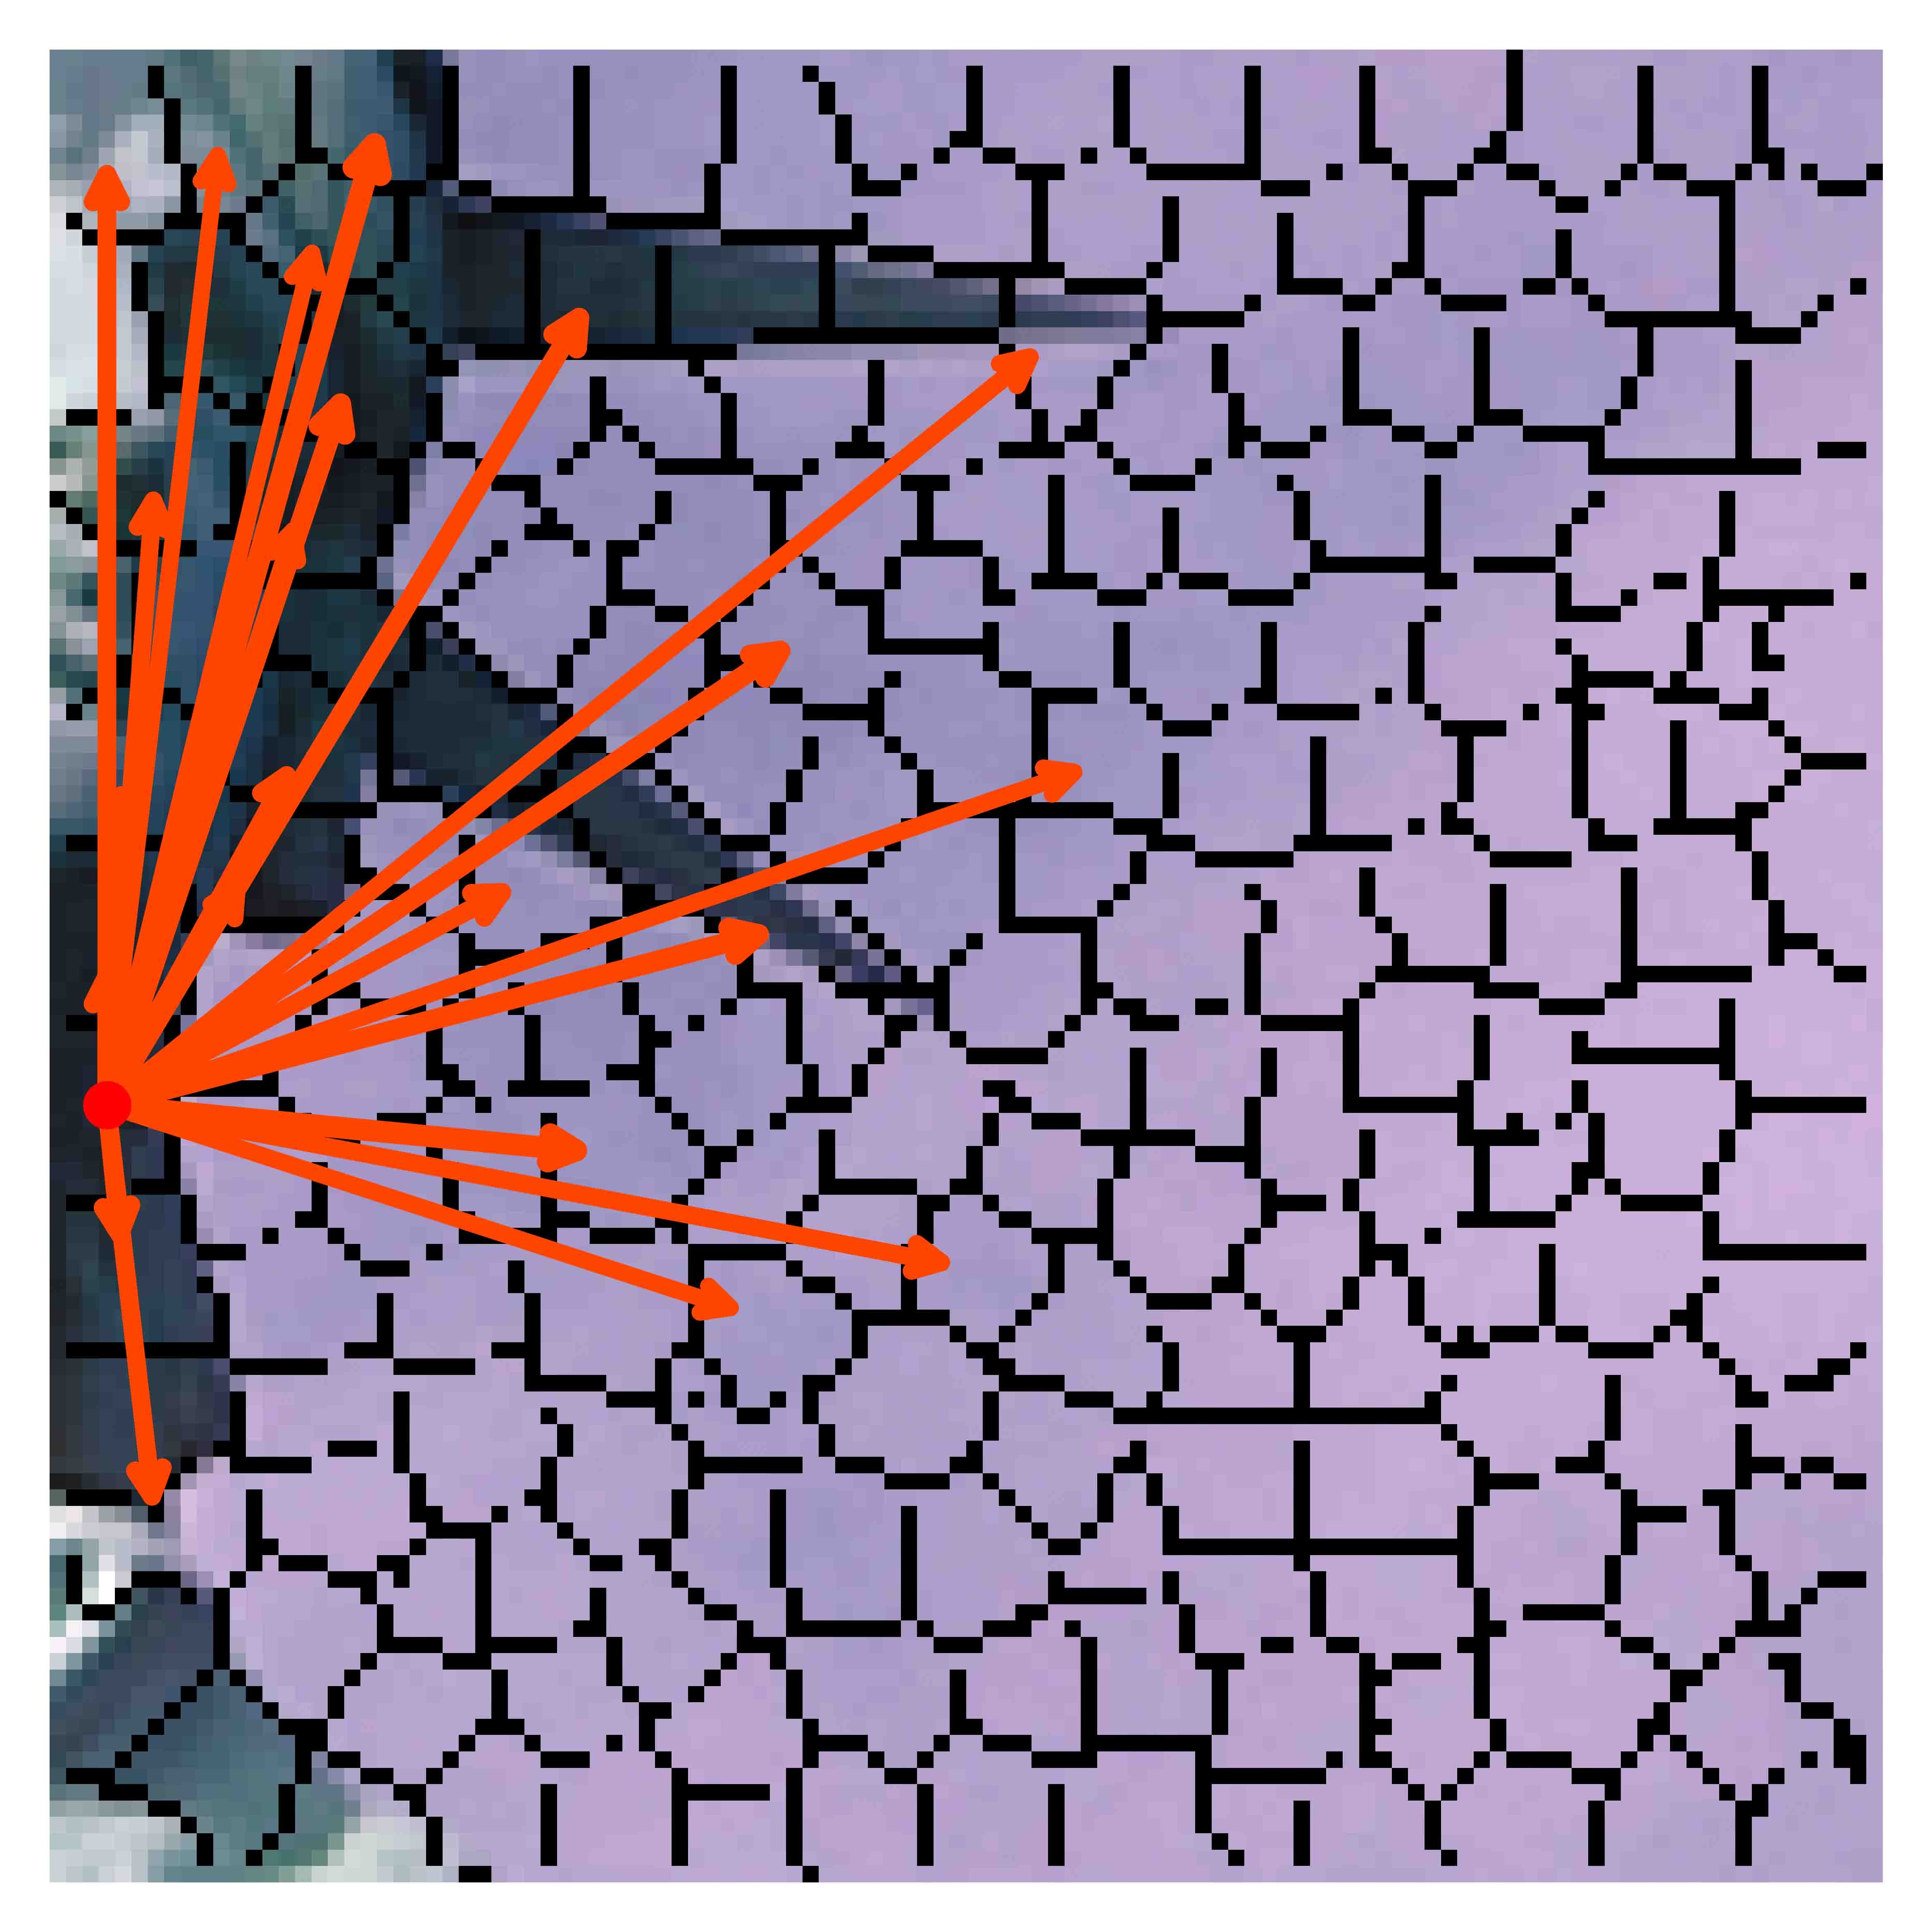
\includegraphics[width=1.5in]{cropped/lady_superpixel_10.jpg}
		\centerline{(k)}
	\end{minipage}
	\begin{minipage}[t]{.24\linewidth}
		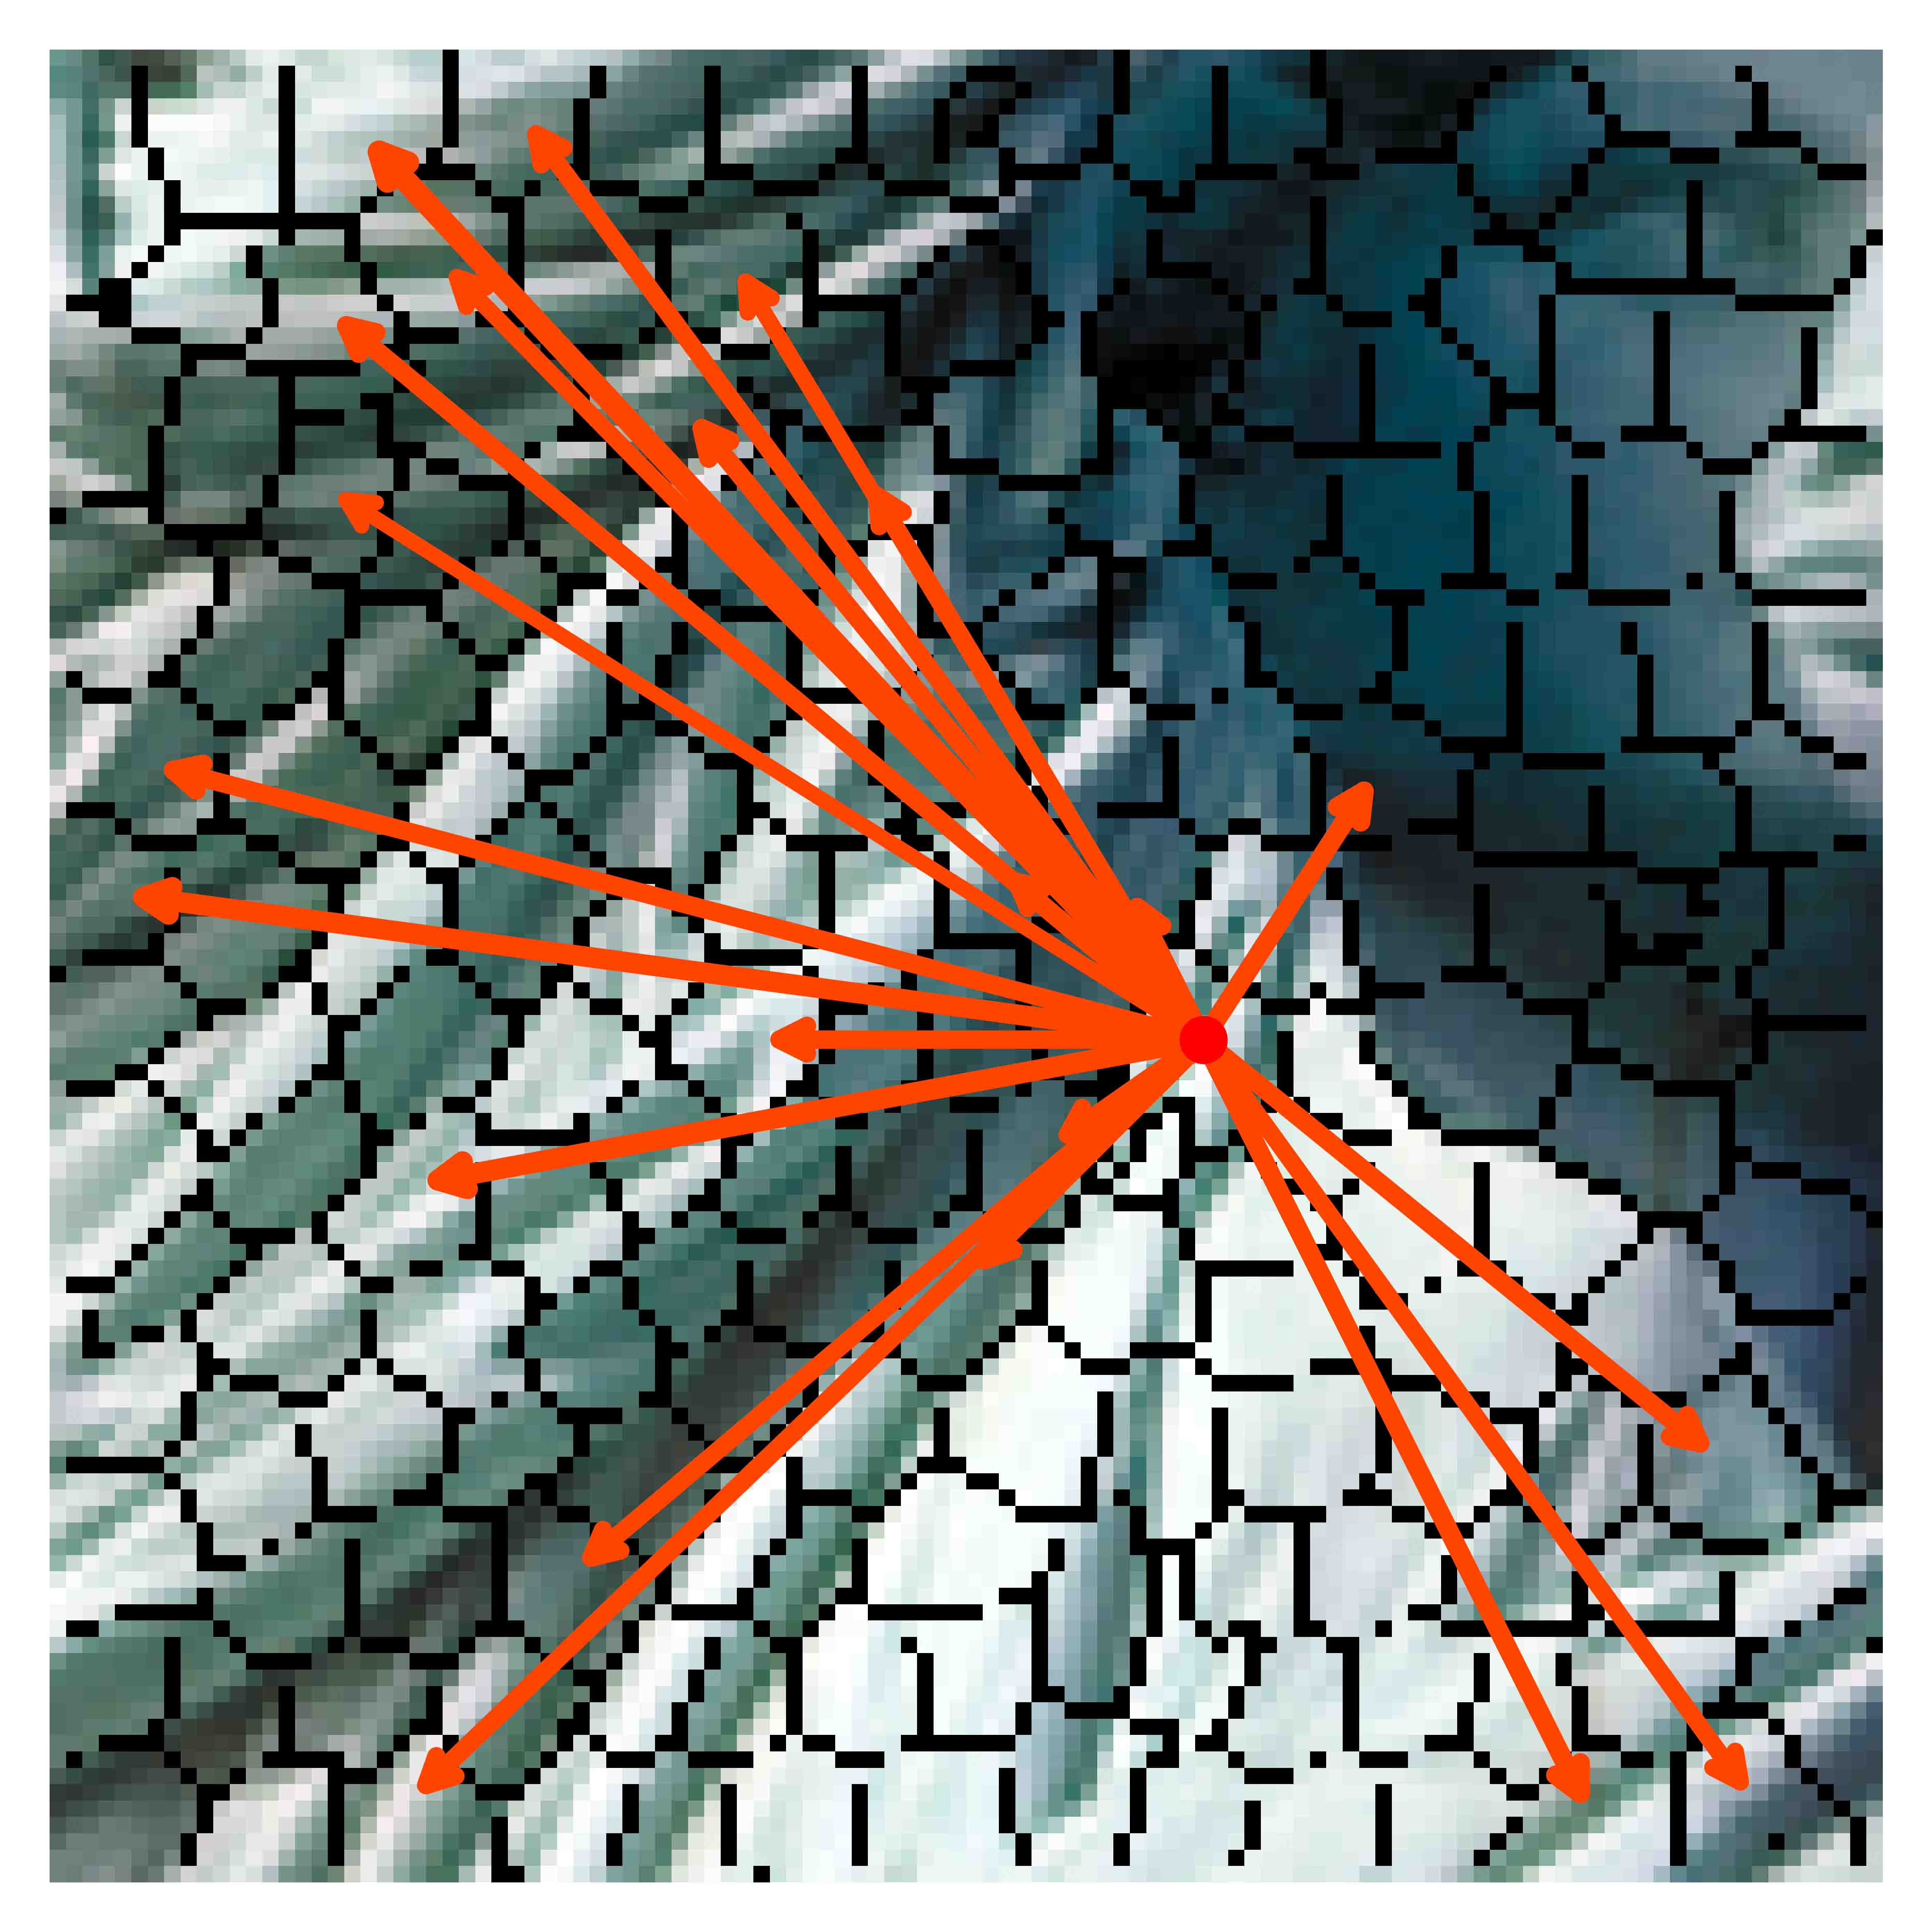
\includegraphics[width=1.5in]{cropped/lady_superpixel_9.jpg}
		\centerline{(l)}
	\end{minipage}
	\begin{minipage}[t]{.24\linewidth}
		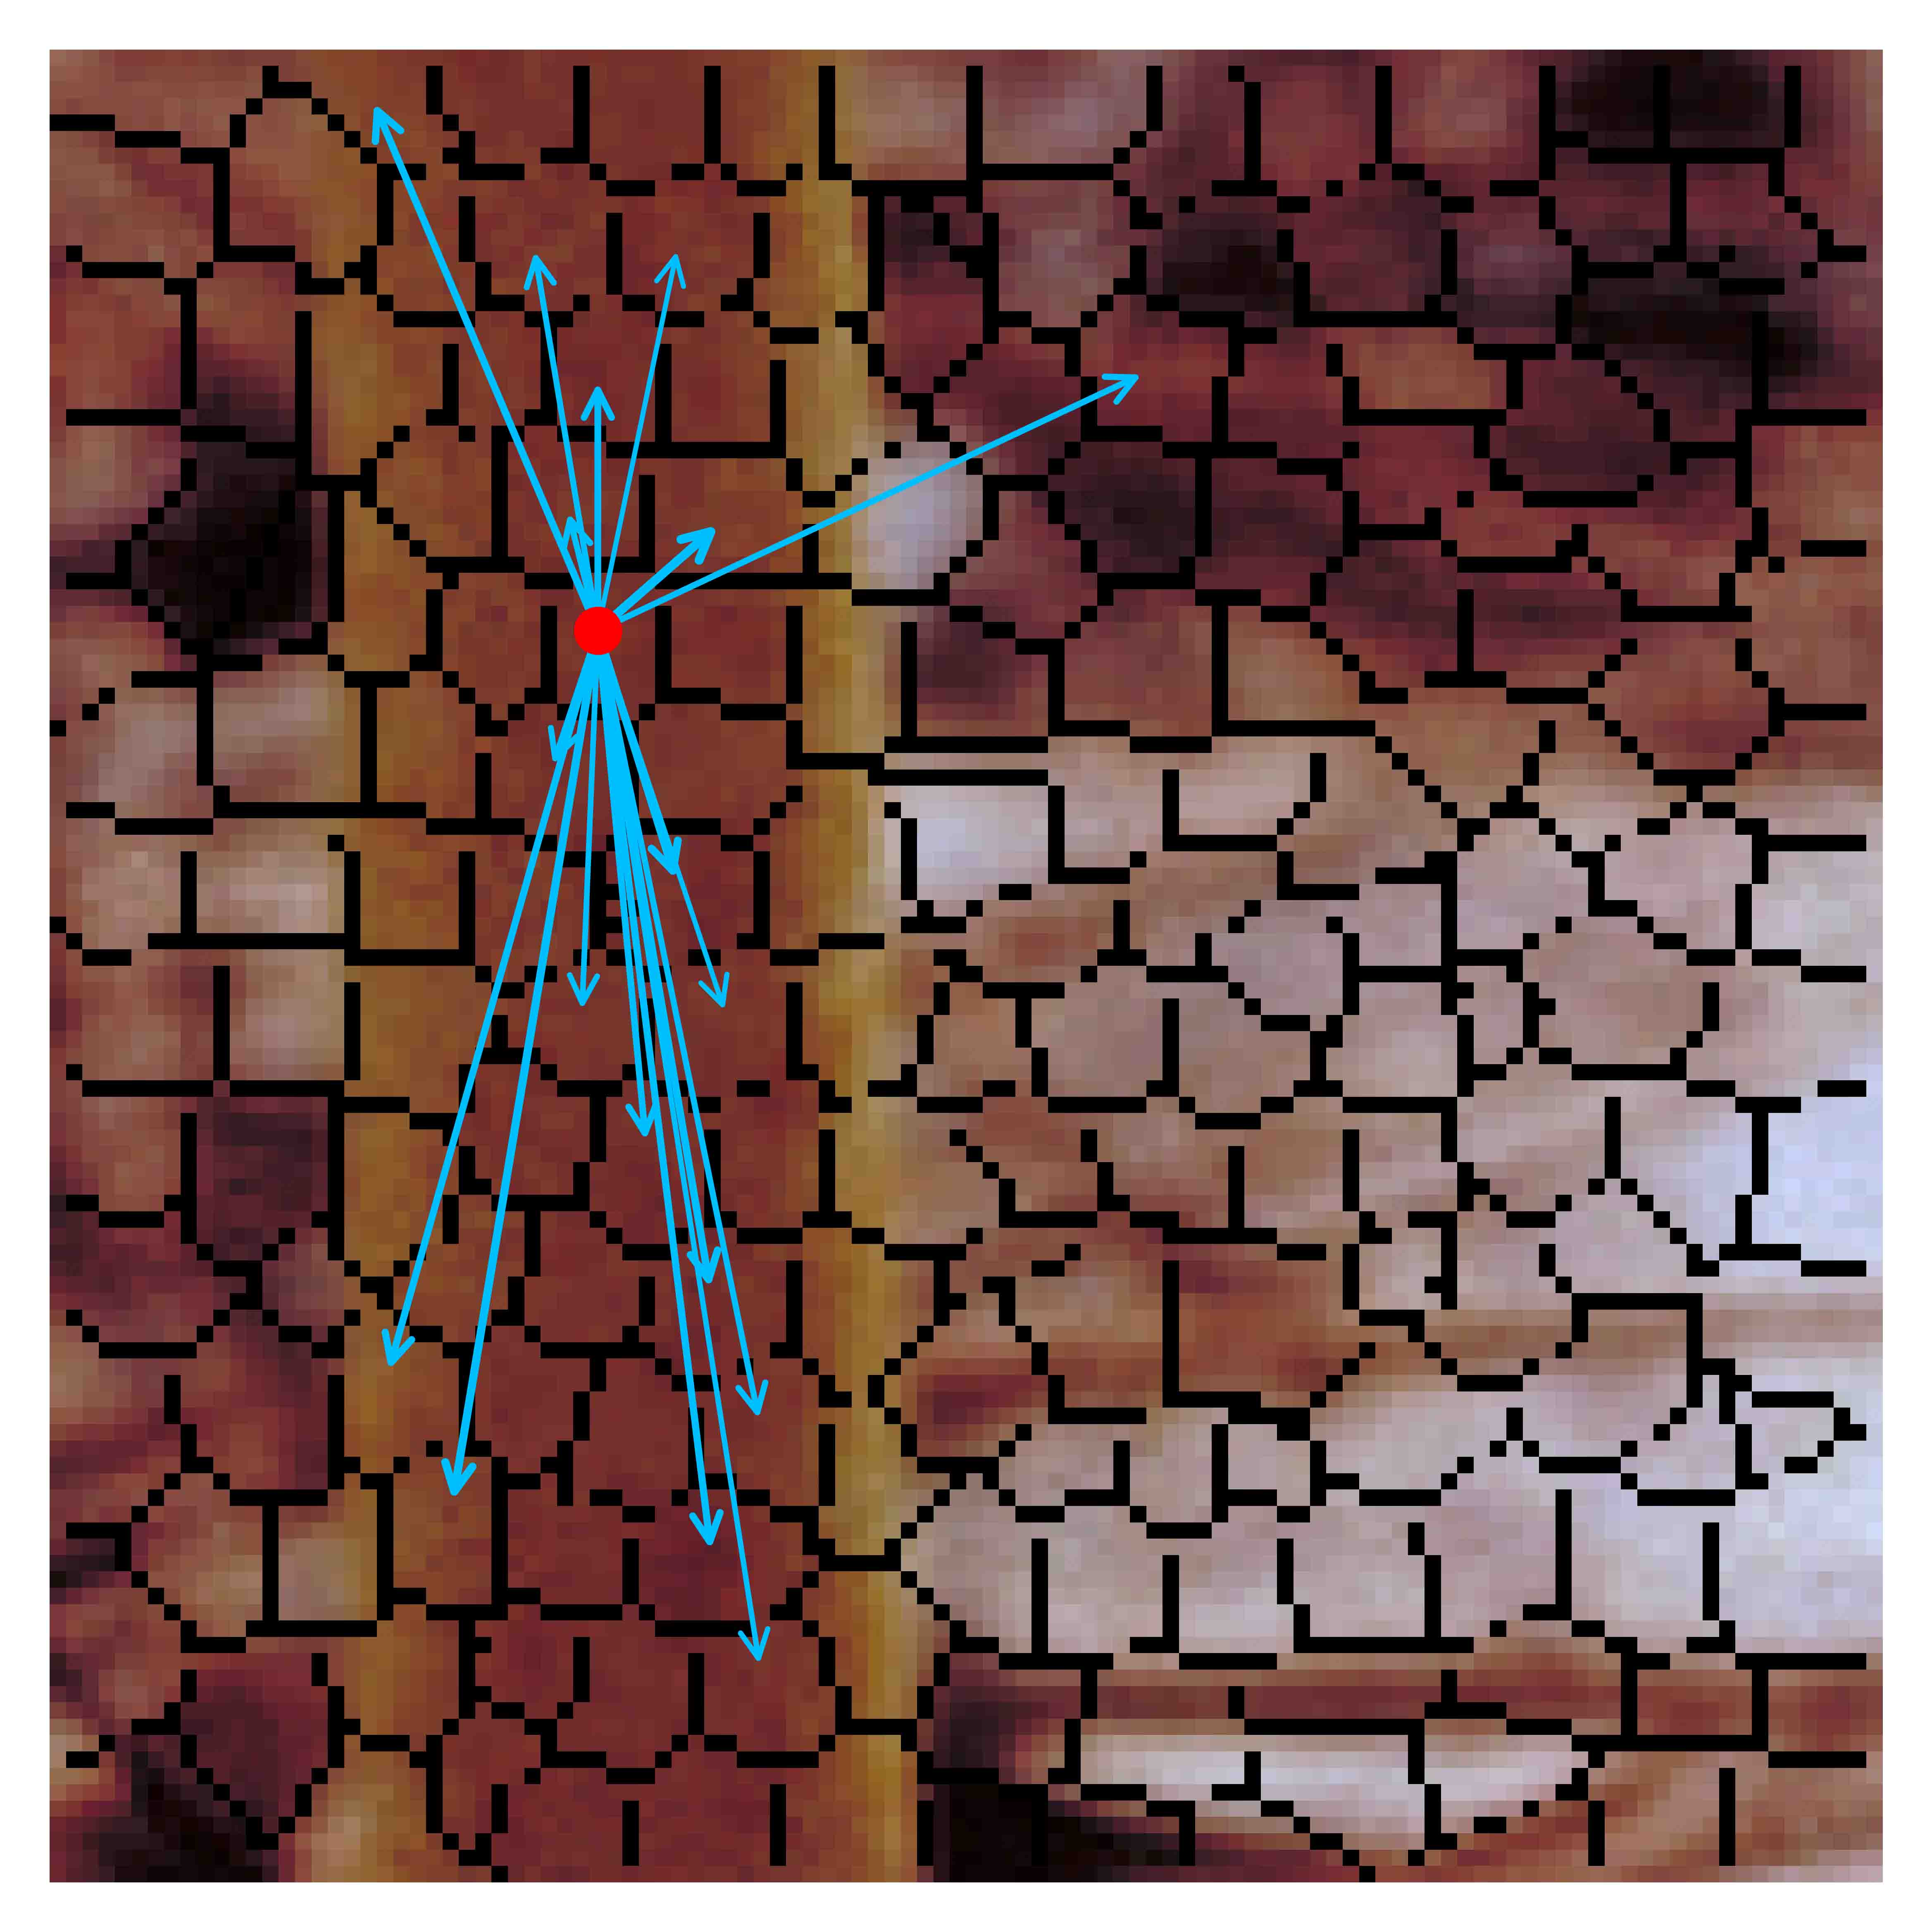
\includegraphics[width=1.5in]{cropped/shroom_superpixel_9.jpg}
		\centerline{(m)}
	\end{minipage}
	\begin{minipage}[t]{.24\linewidth}
		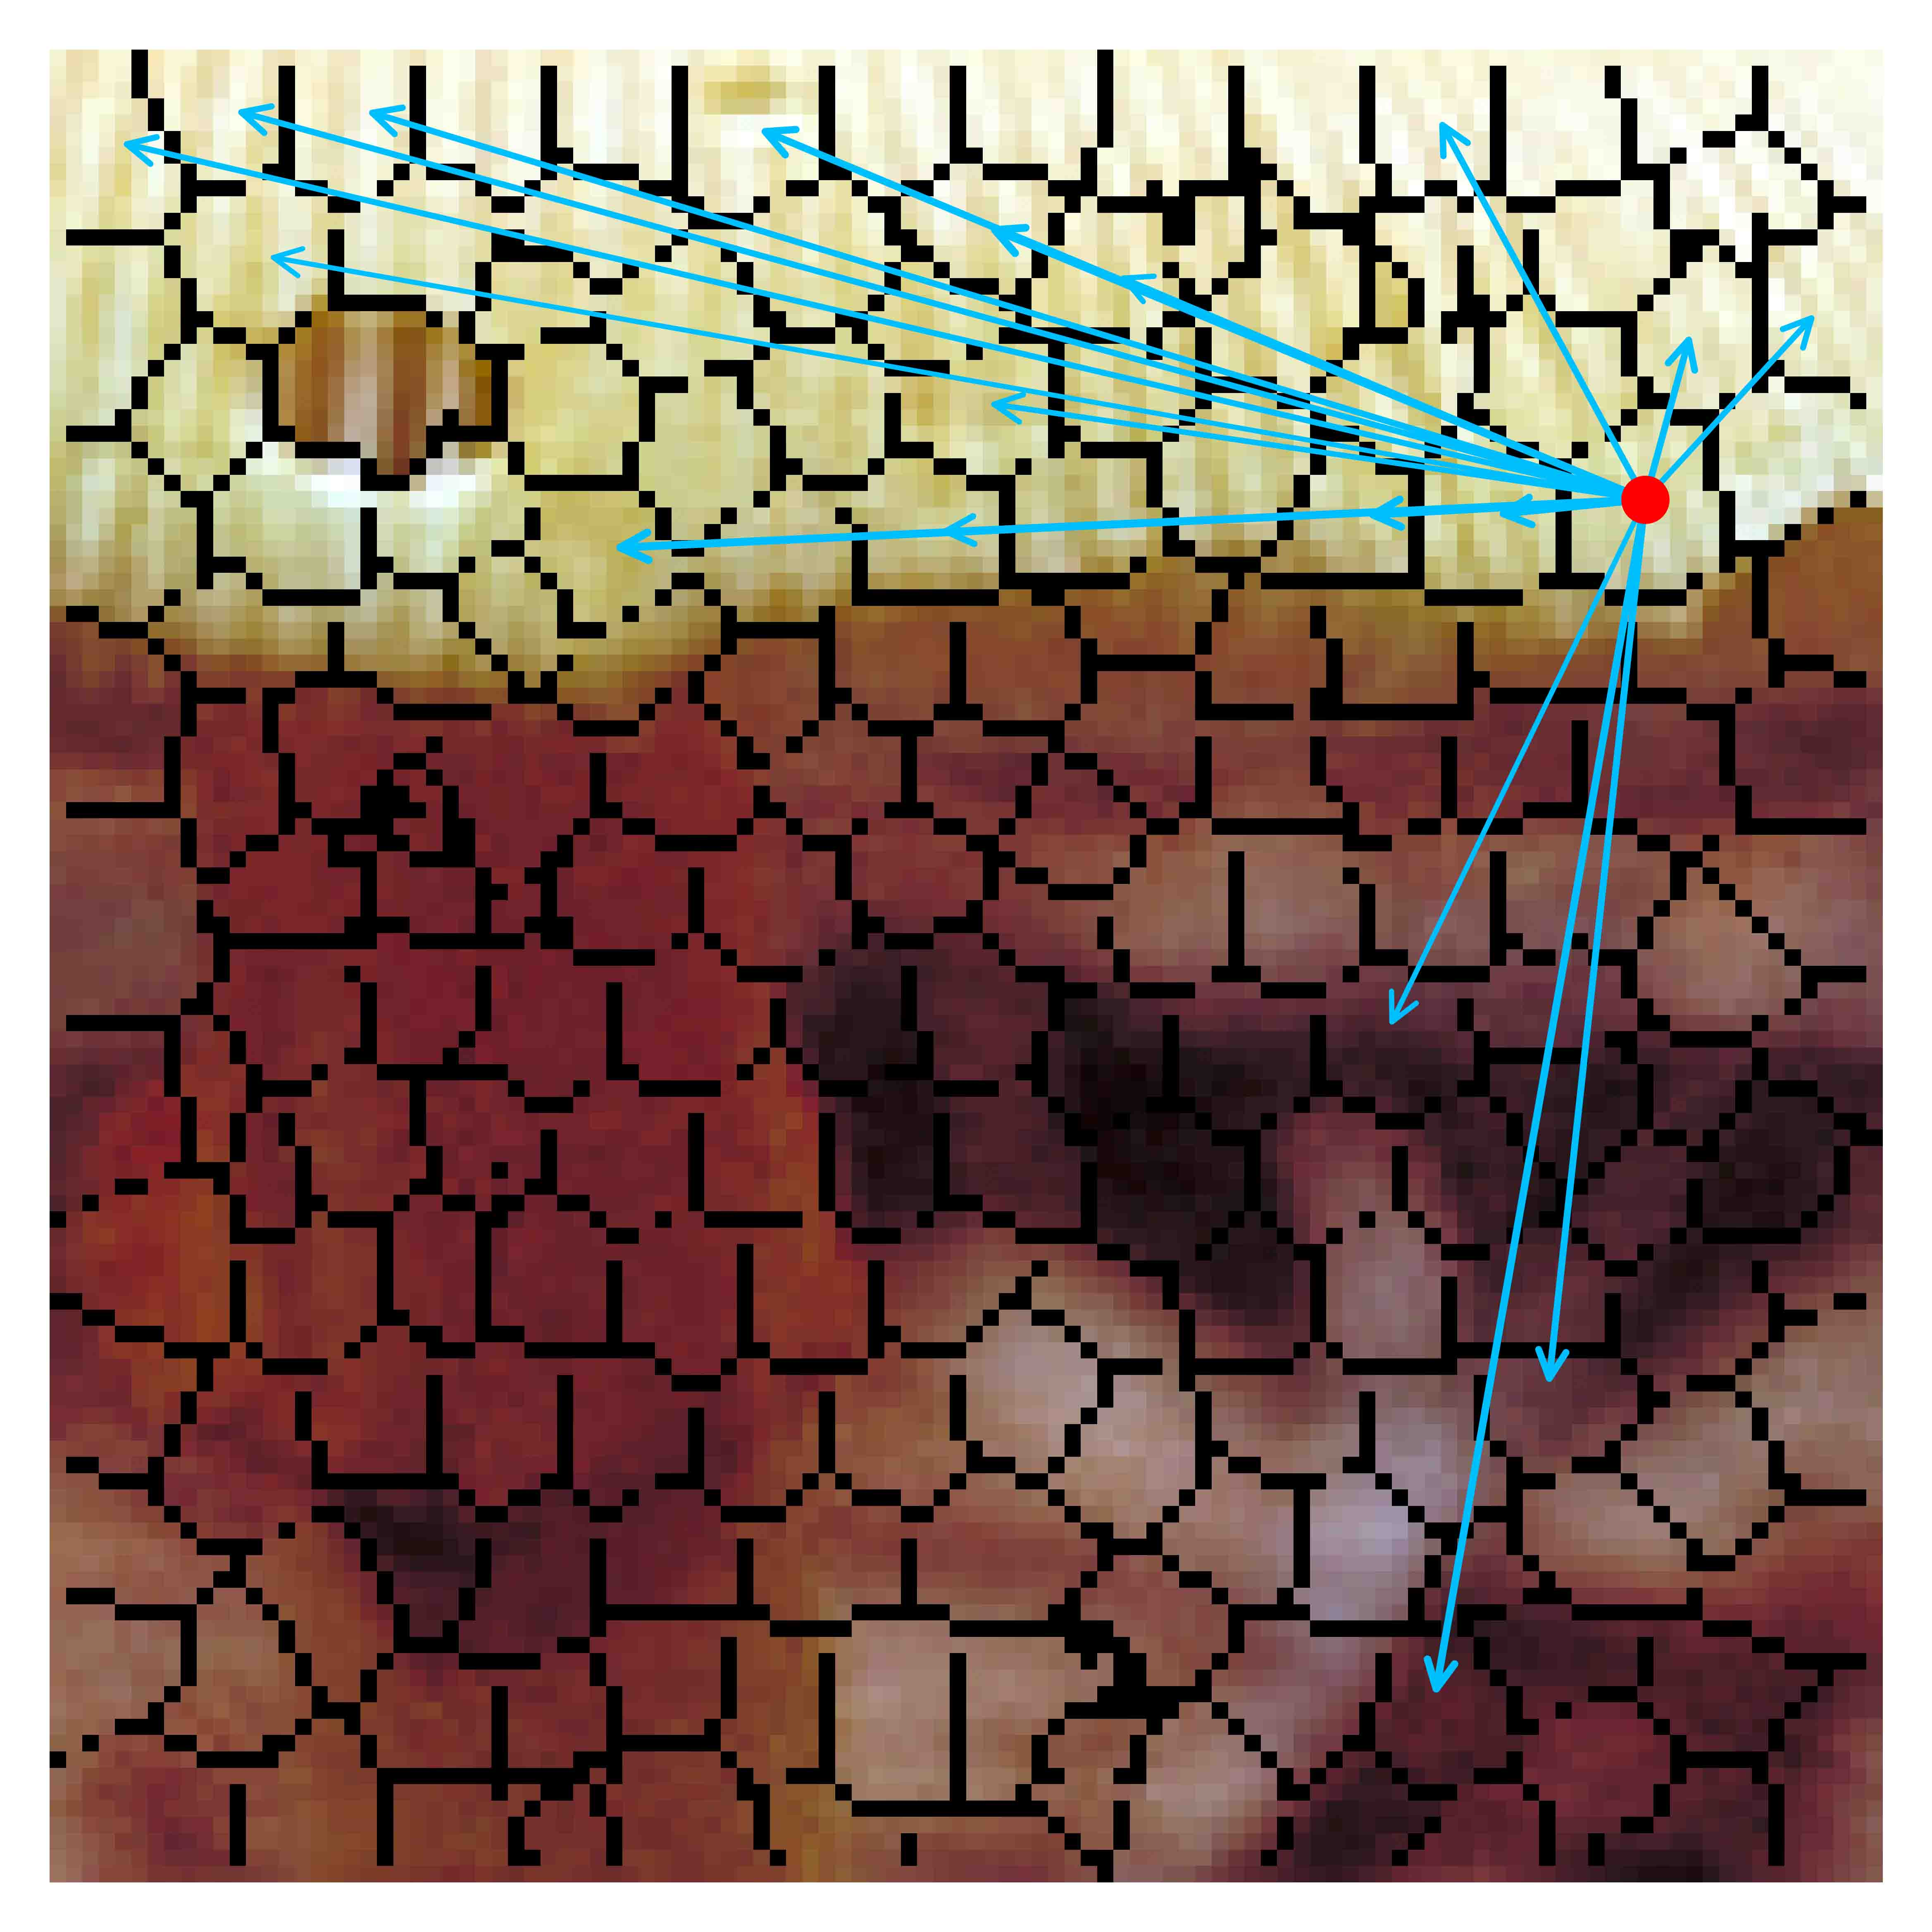
\includegraphics[width=1.5in]{cropped/shroom_superpixel_5.jpg}
		\centerline{(n)}
	\end{minipage}
	\begin{minipage}[t]{.24\linewidth}
		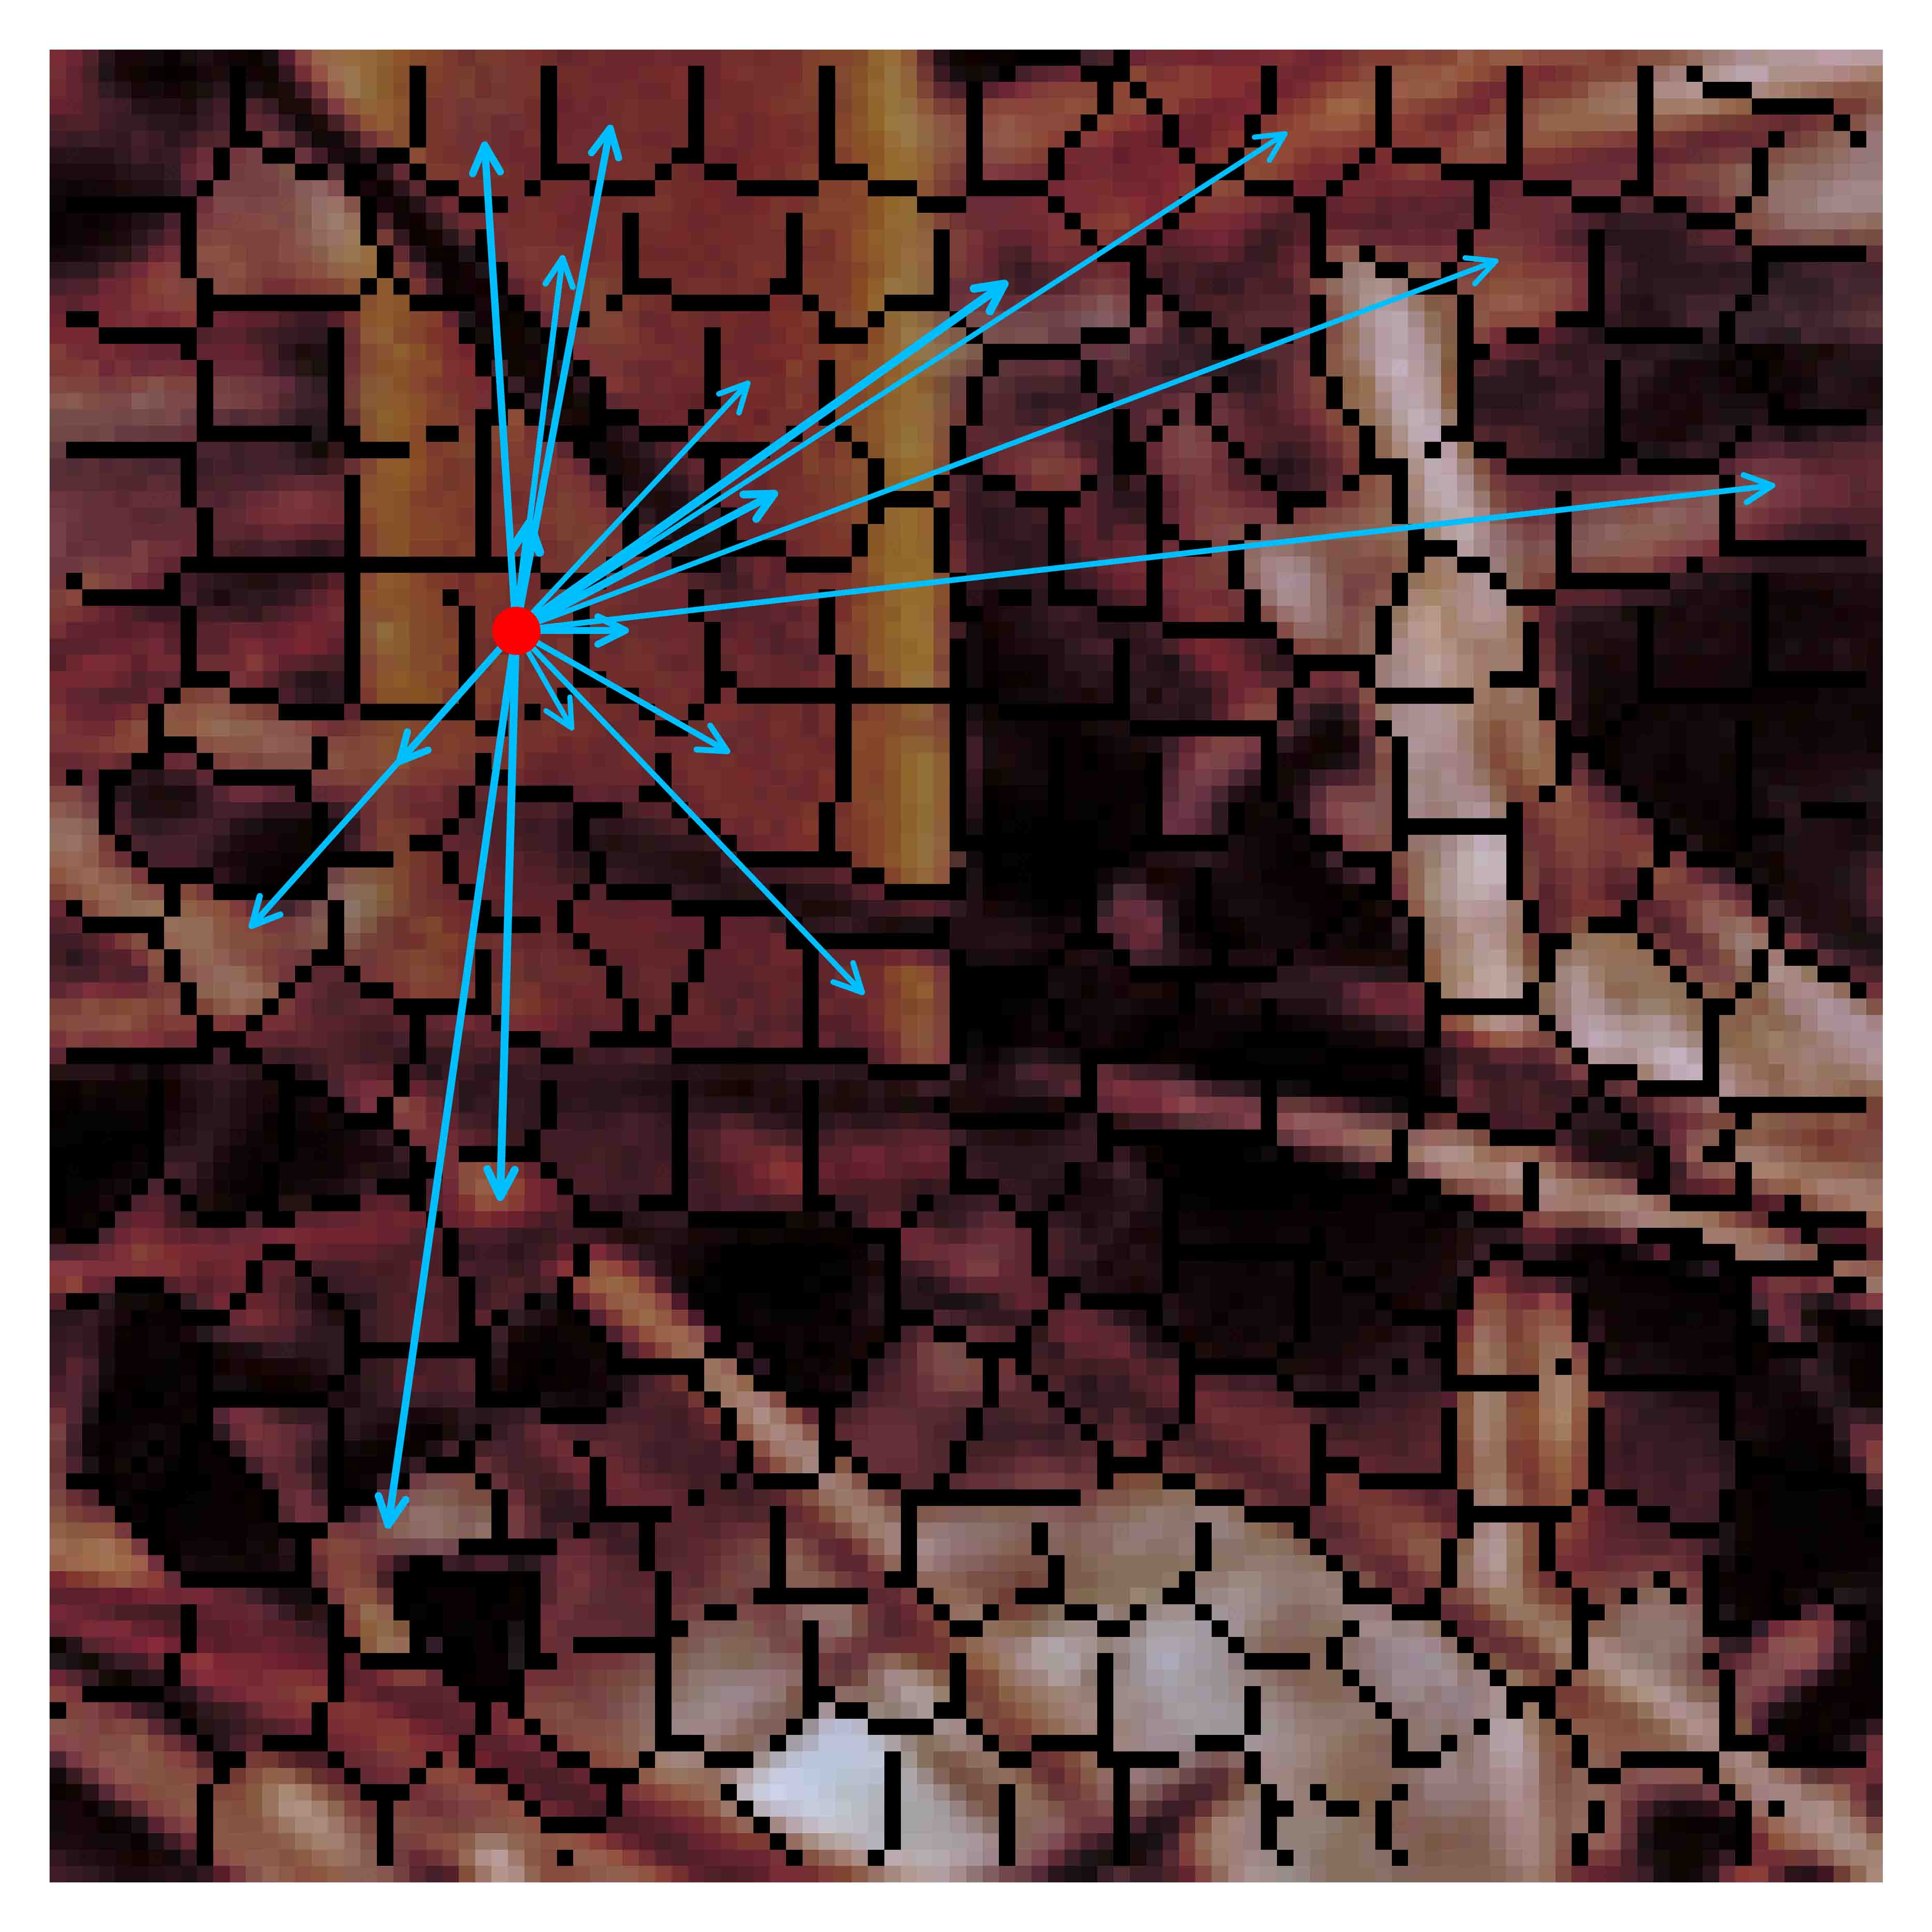
\includegraphics[width=1.5in]{cropped/shroom_superpixel_13.jpg}
		\centerline{(o)}
	\end{minipage}
	\begin{minipage}[t]{.24\linewidth}
		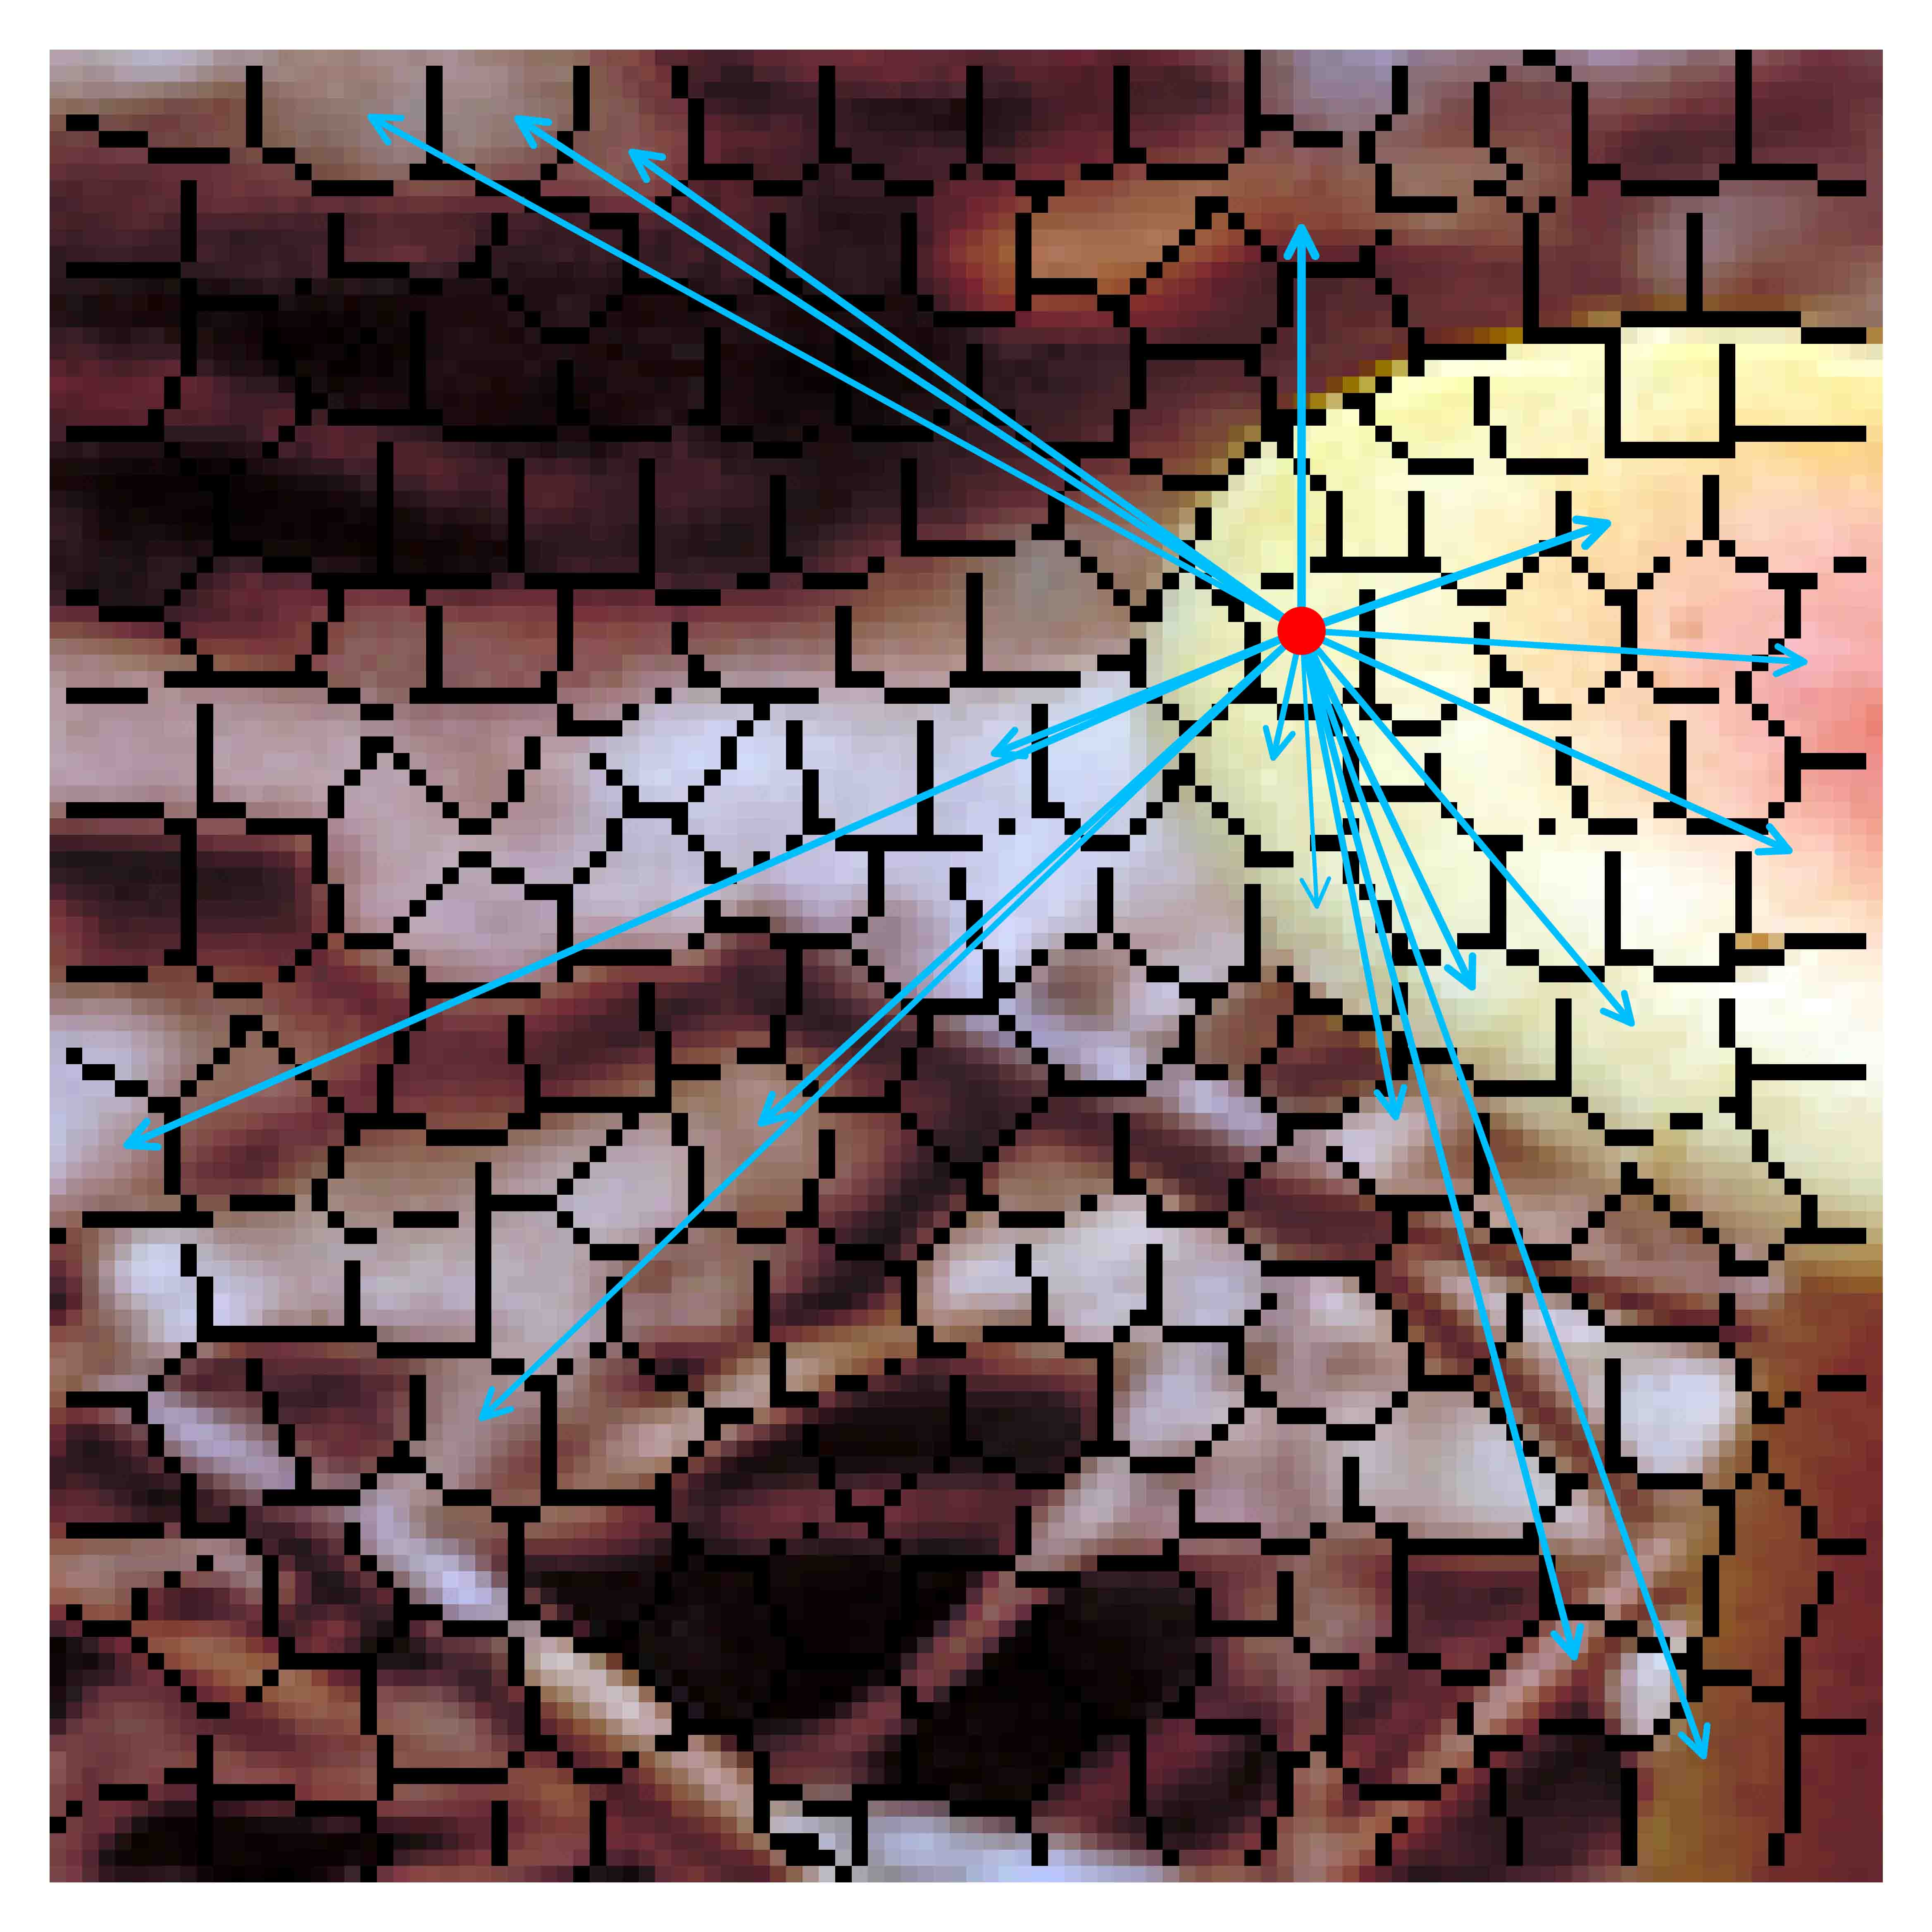
\includegraphics[width=1.5in]{cropped/shroom_superpixel_15.jpg}
		\centerline{(p)}
	\end{minipage}
	\caption{Selected demonstrations of the non-local behavior and long-range dependencies of the cropped image patches from the illustrated images in~\reffig{Non-local Behavior from the TID2013 database}.}
	\label{Non-local Behavior of the cropped patches with superpixels}
\end{figure*}

In this work, we perform the superpixel segmentation on the cropped patches ($112 \times 112$) with the size of superpixels set by $8 \times 8$. The non-local demonstrations are shown in~\reffig{Non-local Behavior of the cropped patches with superpixels}. In the GNN construction phase, we uniformly sample 60 nodes from each superpixel to aggregate local features within superpixels. We apply the cosine similarity among the aggregated features of superpixels to measure the correlations and similarities. To build a graph for non-local feature integration, we empirically set a threshold of 0.70. There is an edge if the similarity between two superpixels is greater than the threshold. Otherwise, there is no connection. We employ the initial connection for each layer to prevent the over-smoothing problem~\citep{chen2020simple}. Besides, half of the total nodes,~\ie, 100 nodes, are uniformly sampled to aggregate the non-local features~\citep{wang2018non}.

We utilize 32 hidden neurons inside ${\mathrm{FC}}(\cdot)$ in~\refequ{concat} to map the input normalized RGB values to a hidden representation. Besides, the number of heads $M$ is set as 4, and the GNN layer is parallelly implemented for stable and faster training. In~\refequ{Normalization}, $C$ is set as 127. In addition, in~\refequ{nodenorm}, we set $p=2$ and $C'$ to $1 \times 10^{-5}$. The number of neurons inside the fully-connected layer for quality prediction and distortion type classification is 512 before the final output layer. The batch size $B$ is 4. We train the model using the Adam optimizer~\citep{kingma2015adam} for 100 epochs over all the experiments with a learning rate $\eta=1\times10^{-4}$ which is reduced by 5 every 20 epochs. In~\refequ{loss}, the weight decay rate $\rho$ is $5\times10^{-4}$, and $\theta$ is set as 100.

\subsection{Evaluation Databases and Criteria}
\subsubsection{Evaluation Databases}
\begin{table*}[!ht]
	\centering
	\caption{Brief summary of the LIVE, CSIQ, TID2013, and KADID-10k databases.}
	\label{database}
	\resizebox{\linewidth}{!}{
		\begin{tabular}{lcccc}
			\toprule
			Database & LIVE~\citep{livedataset} & CSIQ~\citep{larson2010most} & TID2013~\citep{ponomarenko2015image} & KADID-10k~\citep{kadid10k} \\ 
			\midrule
			Num. of Reference Images & 29 & 30 & 25 & 81 \\
			Num. of Distorted Images & 779 & 866 & 3,000 & 10,125 \\
			Num. of Distortion Types & 5 & 6 & 24 & 25 \\
			Num. of Distortion Levels & $5 \sim8 $ & $3 \sim 5$ & 5 & 5 \\
			Annotation & DMOS & DMOS & MOS & MOS \\
			Range & [0, 100] & [0, 1] & [0, 9] & [1, 5] \\
			\bottomrule
		\end{tabular}
	}
\end{table*}
The proposed NLNet is evaluated on four natural image IQA benchmarks, including LIVE~\citep{livedataset}, CSIQ~\citep{larson2010most}, TID2013~\citep{ponomarenko2015image}, and KADID-10k~\citep{kadid10k} databases. In~\reftab{database}, a lower DMOS indicates a better quality, whereas the MOS is the opposite.

\paragraph{LIVE} The Laboratory of Image and Vision Engineering (LIVE) public-domain subjective image quality database contains 779 distorted images from 29 reference images of various sizes from $438 \times 634$ to $512 \times 768$. There are 5 distortion types, and each corresponds to 5 $\sim$ 8 distortion levels. The 5 distortion types are JPEG 2000 compression (JP2K, 169 images), JPEG compression (JPEG, 175 images), white noise (WN, 144 images), Gaussian blur (GB, 144 images), and fast fading Rayleigh (FF, 144 images). 29 observers' single-stimulus ratings are collected and converted to the DMOS, and then quality scores are scaled between 0 and 100. The format of the images is BMP.

\paragraph{CSIQ} The categorical image quality database contains 866 distorted images from 30 reference images with the size of $512 \times 512$. There are 6 distortion types. The 6 distortion types are JPEG (150 images), JP2K (150 images), GB (150 images), WN (150 images), global contrast decrements (CC, 116 images), and additive pink Gaussian noise (PN, 150 images). The CC distortion type corresponds to $3 \sim 5$ distortion levels, and other distortion types all correspond to 5 distortion levels. 35 observers' ratings are normalized to the DMOS between 0 and 1. The format of the images is PNG.

\paragraph{TID2013} The Tampere Image Database (TID) contains 3000 distorted images from 25 reference images with the size of $384 \times 512$. There are 24 distortion types and 5 distortion levels. The 24 distortion types are additive Gaussian noise, lossy compression of noisy images, spatially correlated noise, high frequency noise, impulse noise, quantization noise, GB, image denoising, JPEG, JP2K, multiplicative WN, image color quantization with dither, sparse sampling and reconstruction, JPEG transmission errors, JPEG 2000 transmission errors, additive noise in color components, non eccentricity pattern noise, comfort noise, contrast change, change of color saturation, chromatic aberrations, masked noise, local bock-wise distortions with different intensity, and mean shift (intensity shift). 985 observers' double-stimulus ratings are collected and scaled to the MOS between 0 and 9. The format of the images is BMP.

\paragraph{KADID-10k} The Konstanz Artificially Distorted Image quality Database (KADID) contains 10,125 distorted images and 81 reference images with the size of $384 \times 512$. There are 25 distortion types, and each corresponds to 5 distortion levels. The 25 distortion types are blurs (lens blur, motion blur, and GB), color distortions (color diffusion, color shift, color saturation 1, color saturation 2, and color quantization), compression (JPEG and JP2K), noise (impulse noise, denoise, WN, white noise in color component, and multiplicative noise), brightness change (brighten, darken, and mean shift), spatial distortions (jitter, pixelate, non-eccentricity patch, quantization, and color block), and sharpness and contrast (high sharpen and contrast change). 2,209 observers' ratings are converted to the MOS between 1 and 5. The format of the images is PNG.

\subsubsection{Experiments Settings}\label{Experiments Settings}
For intra-database experiments, we randomly split the reference images into 60\% training, 20\% validation, and 20\% testing, and 10 random splits of the reference indices are performed to avoid bias. We report the median performances on the testing set. Furthermore, for the cross-database experiments, one database is used as the training set, and the other databases are the testing sets. The performance of the model in the last epoch is reported. The images are cropped to several patches with the size of $112 \times 112$ during training. All the cropped patches are utilized in the testing phase, and the final prediction results are their average. The Pearson Linear Correlation Coefficient (PLCC) and Spearman Rank-order Correlation Coefficient (SRCC) are used to evaluate model performance. The proposed model will be more accurate if the PLCC and SRCC are closer to 1.

The PLCC is applied to measure the prediction accuracy.

\begin{equation}
	\mathrm{PLCC}=\frac{\sum\limits_{i=1}^{n}\left(s_{i}-\bar{s}\right)\left(q_{i}-\bar{q}\right)}{\sqrt{\sum\limits_{i=1}^{n}\left(s_{i}-\bar{s}\right)^{2}} \sqrt{\sum\limits_{i=1}^{n}\left(q_{i}-\bar{q}\right)^{2}}},
\end{equation}
in which $s_{i}$ and $q_{i}$ are subjective score,~\ie, MOS or DMOS, and the predicted quality score of the $i^{th}$ image. $\bar{s}$ and $\bar{q}$ are the mean values of $\boldsymbol{\mathrm{s}}$ and $\boldsymbol{\mathrm{q}}$. $n$ is the number of images.

The SRCC measures the prediction monotonicity.

\begin{equation}
	\mathrm{SRCC}=1-\frac{6 \sum\limits_{i=1}^{n} d_{i}^{2}}{n\left(n^{2}-1\right)},
\end{equation}
where $d_{i}$ denotes the difference between the subjective score (MOS/DMOS) $s_{i}$ and the predicted score $q_{i}$.

\subsection{Performance Evaluations on Individual Database}
\begin{table*}[!]
	\centering
	\caption{Performance comparisons on the LIVE, CSIQ, and TID2013 databases. \\Top two results are highlighted in bold.}
	\label{Individual Database}
	\resizebox{\linewidth}{!}{
		\begin{tabular}{lcccccc}
			\toprule
			\multirow{2}{*}{Method} & \multicolumn{2}{c}{LIVE} & \multicolumn{2}{c}{CSIQ} & \multicolumn{2}{c}{TID2013} \\ 
			& SRCC & PLCC & SRCC & PLCC & SRCC & PLCC \\ 
			\midrule
			BRISQUE (2012)~\citep{mittal2012no} & 0.939 & 0.935 & 0.746 & 0.829 & 0.604 & 0.694 \\
			CORNIA (2012)~\citep{ye2012unsupervised} & 0.947 & 0.950 & 0.678 & 0.776 & 0.678 & 0.768 \\
			M3 (2015)~\citep{xue2014blind} & 0.951 & 0.950 & 0.795 & 0.839 & 0.689 & 0.771 \\
			HOSA (2016)~\citep{xu2016blind} & 0.946 & 0.947 & 0.741 & 0.823 & 0.735 & 0.815 \\
			FRIQUEE (2017)~\citep{ghadiyaram2017perceptual} & 0.940 & 0.944 & 0.835 & 0.874 & 0.68 & 0.753 \\
			DIQaM-NR (2018)~\citep{bosse2017deep} & 0.960 & \textbf{0.972} & - & - & 0.835 & 0.855 \\
			DB-CNN (2020)~\citep{zhang2018blind} & 0.968 & \textbf{0.971} & \textbf{0.946} & \textbf{0.959} & 0.816 & 0.865 \\
			HyperIQA (2020)~\citep{su2020blindly} & 0.962 & 0.966 & 0.923 & 0.942 & 0.729 & 0.775 \\
			GraphIQA (2022)~\citep{sun2022graphiqa} & \textbf{0.968} & 0.970 & 0.920 & 0.938 & - & - \\
			TReS (2022)~\citep{golestaneh2021no} & \textbf{0.969} & 0.968 & 0.922 & 0.942 & \textbf{0.863} & \textbf{0.883} \\ 
			\tabincell{c}{\textbf{NLNet}} & 0.962 & 0.963 & \textbf{0.941} & \textbf{0.958} & \textbf{0.856} & \textbf{0.880} \\ 
			\bottomrule
		\end{tabular}
	}
\end{table*}
In~\reftab{Individual Database}, we present the performance comparisons with several NR-IQA methods. The reported performances are derived from the corresponding papers. We report the results of the DIQaM-NR from~\citep{bosse2017deep} which is the no-reference DIQaM model. From the table, we can observe that the deep-learning based methods, such as the DB-CNN~\citep{zhang2018blind}, HyperIQA~\citep{su2020blindly}, and TReS~\citep{golestaneh2021no}, usually achieve superior performances than the handcrafted feature based methods, as more quality-aware features can be learned from the data. Compared with the GraphIQA~\citep{sun2022graphiqa} where the GNN is also utilized, we achieve a significant SRCC improvement (0.941~\textit{vs.} 0.920) on the CSIQ database. Our method presents a higher subjective opinions consistency than the latest method TReS~\citep{golestaneh2021no} on both the LIVE and CSIQ databases. The comparable performances on the TID2013 and KADID-10k databases further verify the effectiveness of our method. The reason may lie in that the non-local features deliver a robust representation of visual quality.
\begin{table*}[!ht]
	\centering
	\caption{Performance comparisons on the KADID-10k database. \\Top two results are highlighted in bold.}
	\label{KADID}
	\resizebox{\textwidth}{!}{
		\begin{tabular}{lcccccccc}
			\toprule
			Method & \begin{tabular}[c]{@{}c@{}}BRISQUE~\citep{mittal2012no}\end{tabular} & \begin{tabular}[c]{@{}c@{}}CORNIA~\citep{ye2012unsupervised}\end{tabular} & \begin{tabular}[c]{@{}c@{}}HOSA~\citep{xu2016blind}\end{tabular} & \begin{tabular}[c]{@{}c@{}}InceptionResNetV2~\citep{kadid10k}\end{tabular} &
			\begin{tabular}[c]{@{}c@{}}DB-CNN~\citep{zhang2018blind}\end{tabular} &
			\begin{tabular}[c]{@{}c@{}}HyperIQA~\citep{su2020blindly}\end{tabular} & \begin{tabular}[c]{@{}c@{}}TReS~\citep{golestaneh2021no}\end{tabular} & \begin{tabular}[c]{@{}c@{}}\textbf{NLNet}\end{tabular} \\ 
			\midrule
			SRCC & 0.519 & 0.519 & 0.609 & 0.731 & 0.851 & \textbf{0.852} & \textbf{0.859} & 0.846 \\
			PLCC & 0.554 & 0.554 & 0.653 & 0.734 & \textbf{0.856} & 0.845 & \textbf{0.858} & 0.850 \\ 
			\bottomrule
		\end{tabular}
	}
\end{table*}

\subsection{Performance Evaluations of Individual Distortion Type}\label{Performance Evaluations of Individual Distortion Type}
In this subsection, we provide performance comparisons of the individual distortion type on the LIVE, CSIQ, TID2013, and KADID-10k databases in order to further explore and analyze the effectiveness of our proposed method. Distortion types are classified into global distortions and local distortions. Global distortions are the globally and uniformly distributed distortions with non-local recurrences over the image, and local distortions are the local nonuniform-distributed distortions in a local region. The demonstrations of the global and local distortions are shown in~\reffig{LIVE-Distortion-1},~\reffig{LIVE-Distortion-2},~\reffig{TID2013-Distortion}, and~\reffig{KADID-Distortion}.
	
	\subsubsection{Performance Evaluations of Individual Distortion Type on the LIVE Database}
	As shown in~\reftab{individual-LIVE}, we present the average SRCC and PLCC results of the individual distortion type on the LIVE database. The JPEG, JP2K, WN, and GB are globally and uniformly distributed distortions with non-local recurrences, and FF is a local nonuniform-distributed distortion. The global distortions (WN and JPEG) and local distortion (FF) are illustrated with the plane, parrot, butterfly, and motorcyclist images in~\reffig{LIVE-Distortion-1} and~\reffig{LIVE-Distortion-2}. 
	
	Our proposed method has achieved competing performances on all individual distortion types. In specific, compared with the traditional CNN-based methods, such as M3~\citep{xue2014blind}, dipIQ~\citep{ma2017dipiq}, and DB-CNN~\citep{zhang2018blind}, the non-local behavior improves the performance of the globally distorted images with highly competitive SRCC and PLCC results. It indicates the superiority of the non-local modeling methods to handle the globally and uniformly degraded images. Besides, the proposed NLNet obtains state-of-the-art performances on the Gaussian noise-distorted images (0.990 SRCC and 0.993 PLCC). In addition, prediction performance of the compression-related distortions (JPEG and JP2K) is promising. Lastly, our model also achieves comparable performance on the local distortion type,~\ie, FF distortion, revealing that the proposed NLNet manages to handle both global and local distortions.
	\begin{figure*}[!]
		\centering
		\begin{minipage}[t]{.49\linewidth}
			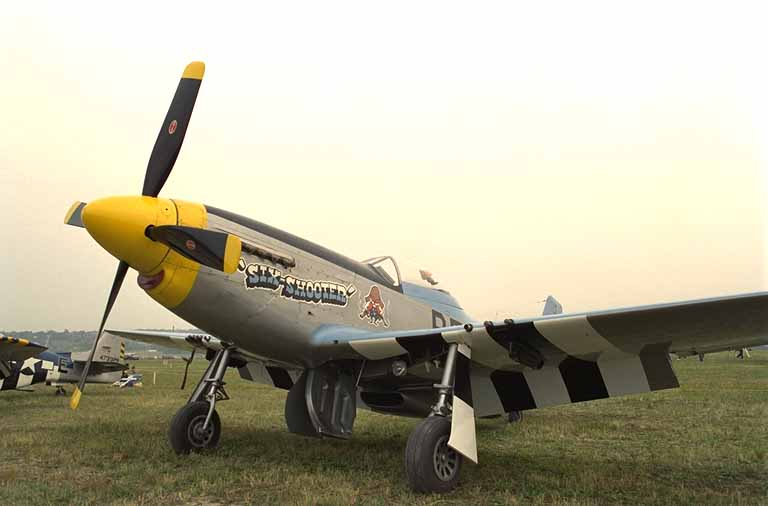
\includegraphics[width=2.8in]{LIVE/REF/plane.jpg}
			\centerline{(a)}
		\end{minipage}
		\begin{minipage}[t]{.49\linewidth}
			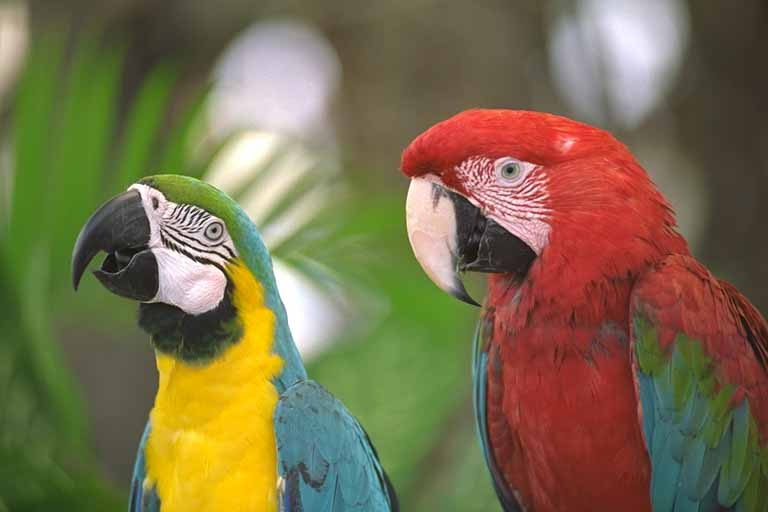
\includegraphics[width=2.8in]{LIVE/REF/parrots.jpg}
			\centerline{(e)}
		\end{minipage}
	
		\begin{minipage}[t]{.49\linewidth}
			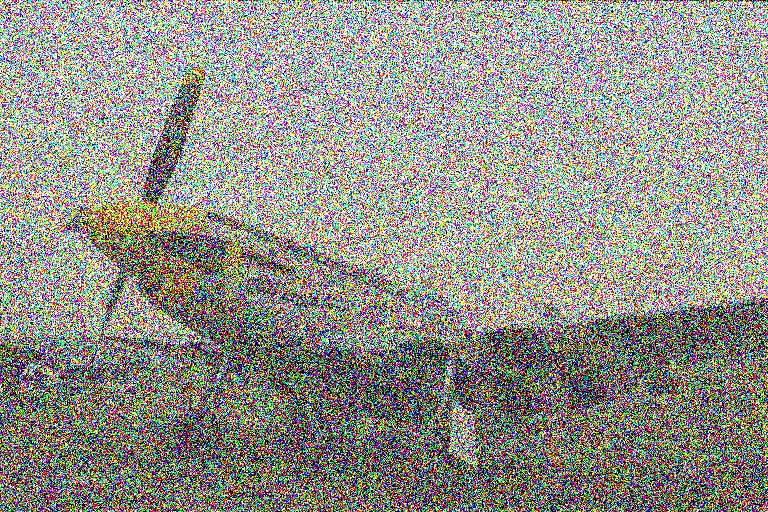
\includegraphics[width=2.8in]{LIVE/WN/img105.jpg}
			\centerline{(b)}
		\end{minipage}
		\begin{minipage}[t]{.49\linewidth}
			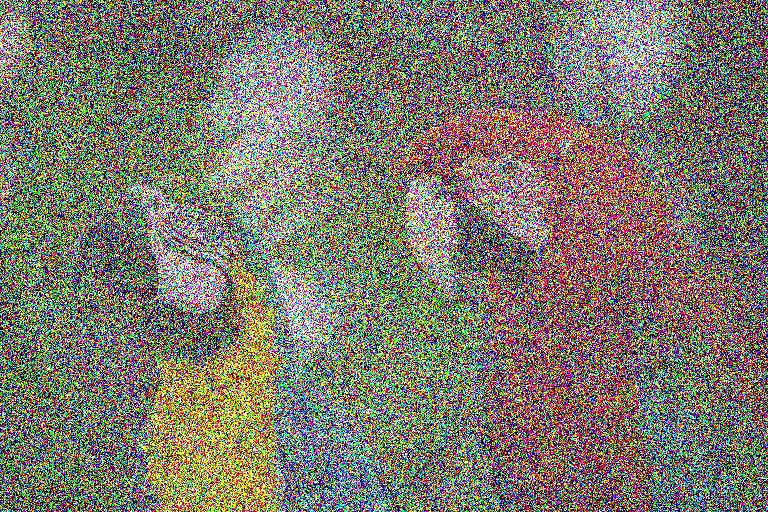
\includegraphics[width=2.8in]{LIVE/WN/img104.jpg}
			\centerline{(f)}
		\end{minipage}
	
		\begin{minipage}[t]{.49\linewidth}
			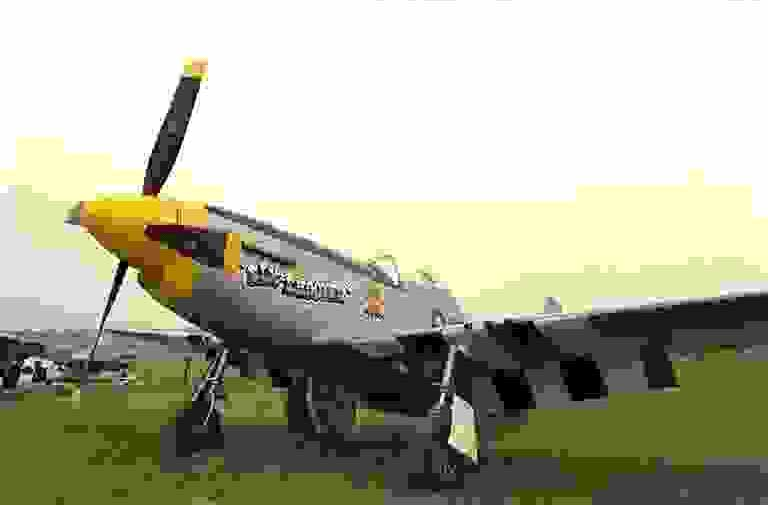
\includegraphics[width=2.8in]{LIVE/JPEG/img201.jpg}
			\centerline{(c)}
		\end{minipage}
		\begin{minipage}[t]{.49\linewidth}
			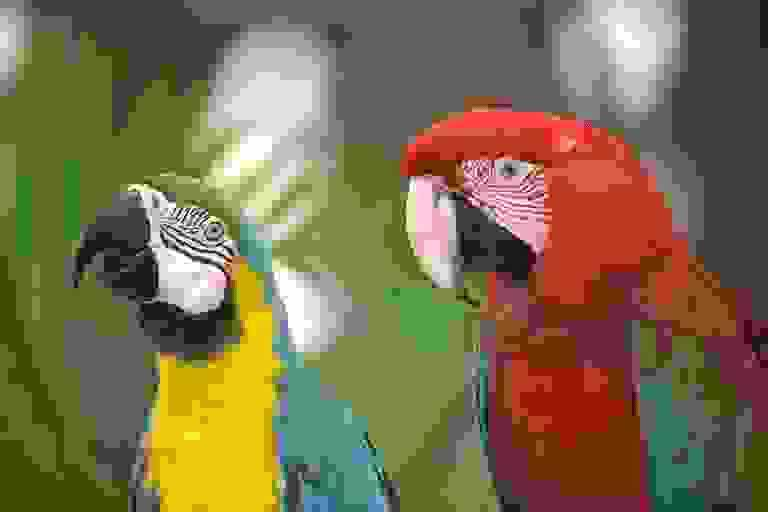
\includegraphics[width=2.8in]{LIVE/JPEG/img233.jpg}
			\centerline{(g)}
		\end{minipage}
	
		\begin{minipage}[t]{.49\linewidth}
			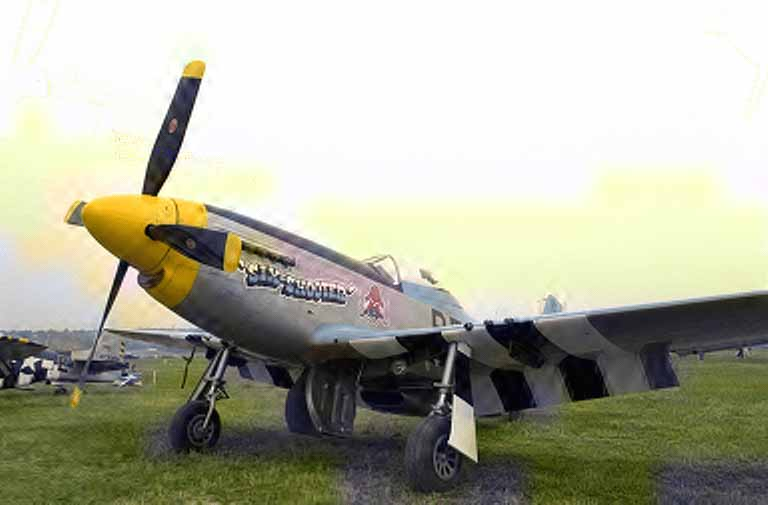
\includegraphics[width=2.8in]{LIVE/FF/img56.jpg}
			\centerline{(d)}
		\end{minipage}
		\begin{minipage}[t]{.49\linewidth}
			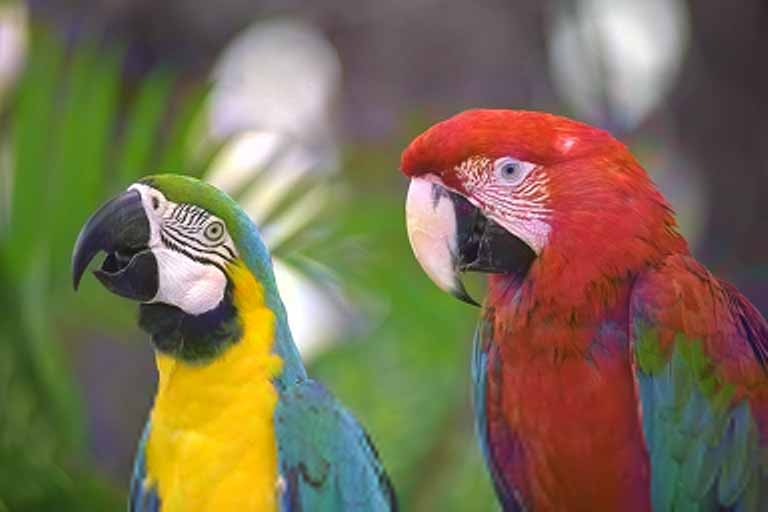
\includegraphics[width=2.8in]{LIVE/FF/img44.jpg}
			\centerline{(h)}
		\end{minipage}
		
		\caption{Demonstrations of the global distortions (b/f: WN and c/g: JPEG) and local distortions (d/h: FF) contaminating the plane and parrot images. Figure (a) and Figure (e) are reference images from the LIVE database.}
		\label{LIVE-Distortion-1}
	\end{figure*}
	\begin{figure*}[!]
		\centering
		\begin{minipage}[t]{.49\linewidth}
			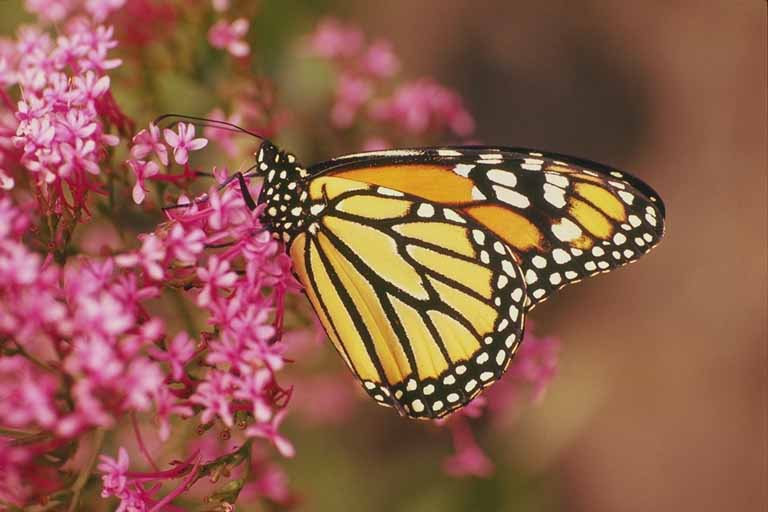
\includegraphics[width=2.8in]{LIVE/REF/monarch.jpg}
			\centerline{(a)}
		\end{minipage}
		\begin{minipage}[t]{.49\linewidth}
			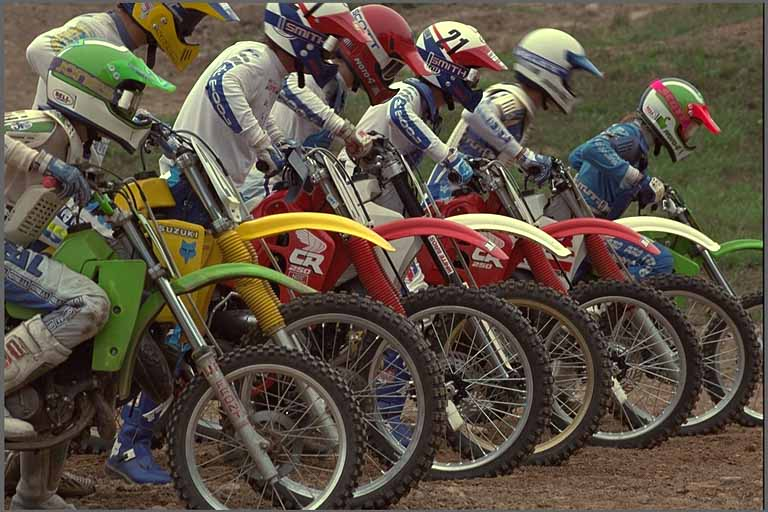
\includegraphics[width=2.8in]{LIVE/REF/bikes.jpg}
			\centerline{(e)}
		\end{minipage}
	
		\begin{minipage}[t]{.49\linewidth}
			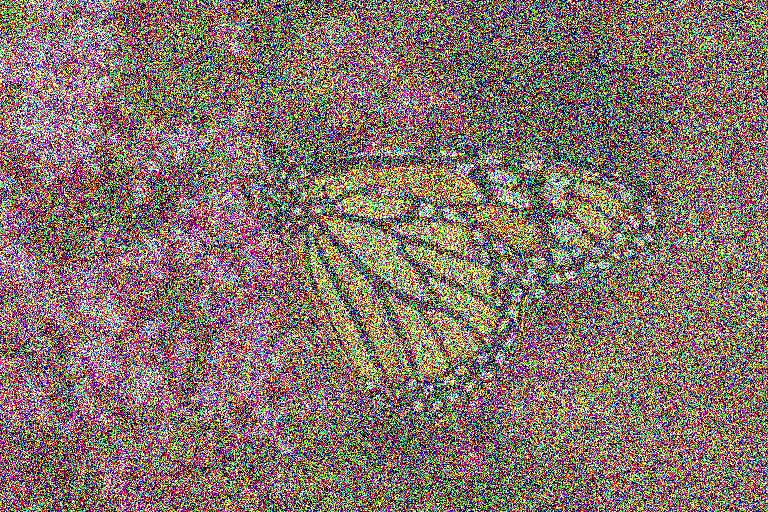
\includegraphics[width=2.8in]{LIVE/WN/img34.jpg}
			\centerline{(b)}
		\end{minipage}
		\begin{minipage}[t]{.49\linewidth}
			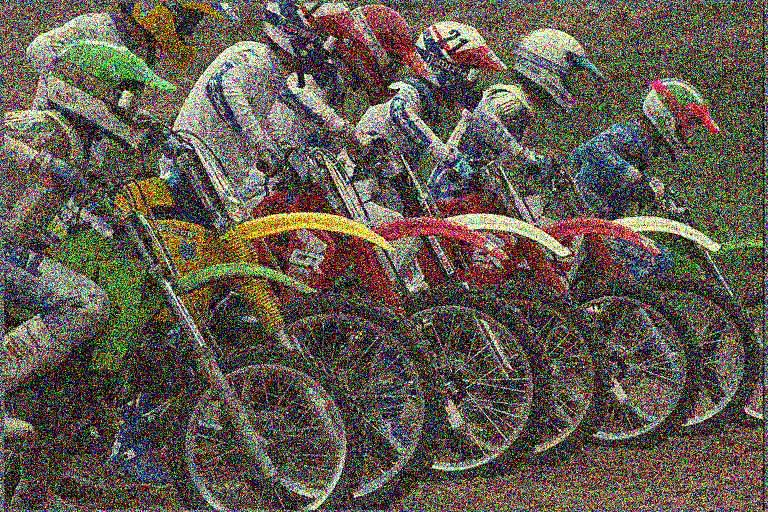
\includegraphics[width=2.8in]{LIVE/WN/img29.jpg}
			\centerline{(f)}
		\end{minipage}
		
		\begin{minipage}[t]{.49\linewidth}
			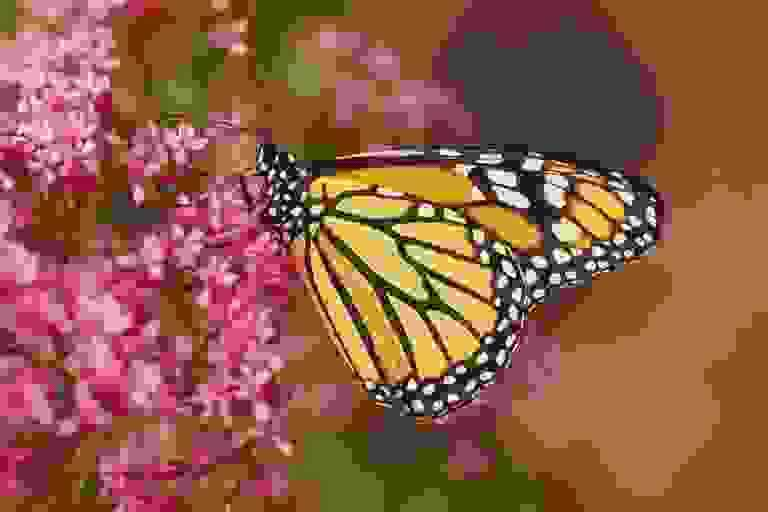
\includegraphics[width=2.8in]{LIVE/JPEG/img170.jpg}
			\centerline{(c)}
		\end{minipage}
		\begin{minipage}[t]{.49\linewidth}
			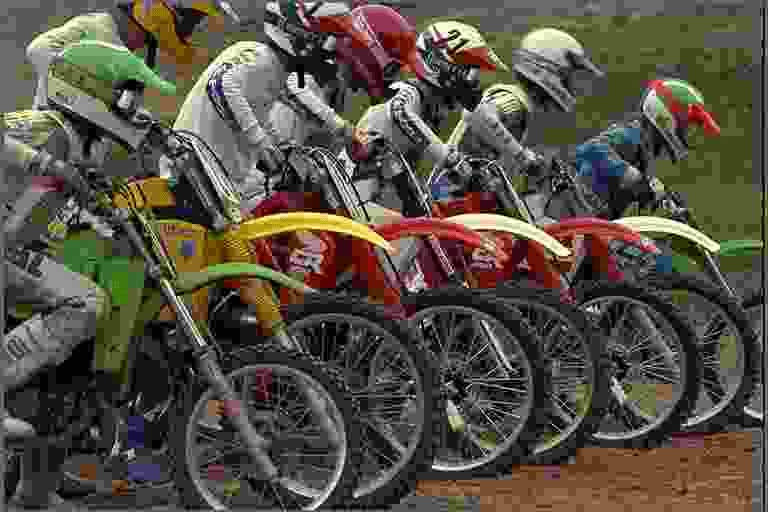
\includegraphics[width=2.8in]{LIVE/JPEG/img29.jpg}
			\centerline{(g)}
		\end{minipage}
	
		\begin{minipage}[t]{.49\linewidth}
			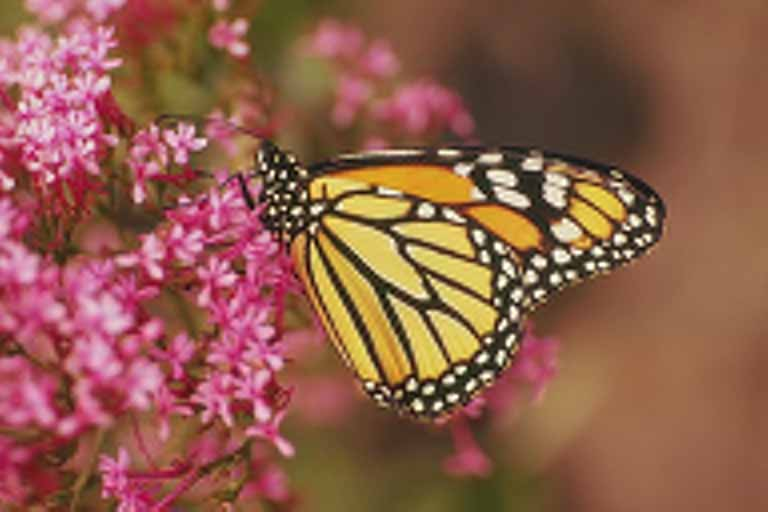
\includegraphics[width=2.8in]{LIVE/FF/img137.jpg}
			\centerline{(d)}
		\end{minipage}
		\begin{minipage}[t]{.49\linewidth}
			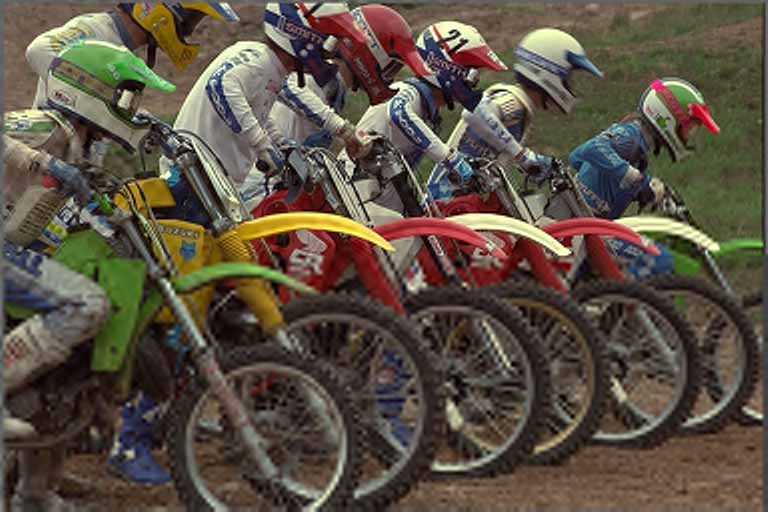
\includegraphics[width=2.8in]{LIVE/FF/img35.jpg}
			\centerline{(h)}
		\end{minipage}
	
		\caption{Demonstrations of the global distortions (b/f: WN and c/g: JPEG) and local distortions (d/h: FF) contaminating the butterfly and motorcyclist images. Figure (a) and Figure (e) are reference images from the LIVE database.}
		\label{LIVE-Distortion-2}
	\end{figure*}
	\begin{table*}[!ht]
		\centering
		\caption{The average SRCC and PLCC results of the individual distortion type on the LIVE database. Top two results are highlighted in bold.}
		\label{individual-LIVE}
		\resizebox{\linewidth}{!}{
			\begin{tabular}{c|cccc|c}
				\toprule
				\multirow{2}{*}{SRCC} & \multicolumn{4}{c|}{Global Distortion} & Local Distortion \\ \cline{2-6} 
				& JPEG & JP2K & WN & GB & FF \\ \midrule
				BRISQUE (2012)~\citep{mittal2012no} & 0.965 & 0.929 & 0.982 & \textbf{0.964} & 0.828 \\
				CORNIA (2012)~\citep{ye2012unsupervised} & 0.947 & 0.924 & 0.958 & 0.951 & 0.921 \\
				M3 (2014)~\citep{xue2014blind} & 0.966 & 0.930 & \textbf{0.986} & 0.935 & 0.902 \\
				HOSA (2016)~\citep{xu2016blind} & 0.954 & 0.935 & 0.975 & 0.954 & \textbf{0.954} \\
				FRIQUEE (2017)~\citep{ghadiyaram2017perceptual} & 0.947 & 0.919 & 0.983 & 0.937 & 0.884 \\
				dipIQ (2017)~\citep{ma2017dipiq} & 0.969 & \textbf{0.956} & 0.975 & 0.940 & - \\
				WaDIQaM (2018)~\citep{bosse2017deep} & 0.953 & 0.942 & 0.982 & 0.938 & 0.923 \\
				DB-CNN (2020)~\citep{zhang2018blind} & \textbf{0.972} & 0.955 & 0.980 & 0.935 & 0.930 \\
				HyperIQA (2020)~\citep{su2020blindly} & 0.961 & 0.949 & 0.982 & 0.926 & 0.934 \\ \midrule
				\begin{tabular}[c]{@{}c@{}}\textbf{NLNet}\end{tabular} & \textbf{0.979} & \textbf{0.958} & \textbf{0.990} & \textbf{0.964} & \textbf{0.941} \\ \toprule
				
				\multirow{2}{*}{PLCC} & \multicolumn{4}{c|}{Global Distortion} & Local Distortion \\ \cline{2-6} 
				& JPEG & JP2K & WN & GB & FF \\ \midrule
				BRISQUE (2012)~\citep{mittal2012no} & 0.971 & 0.940 & 0.989 & \textbf{0.965} & 0.894 \\
				CORNIA (2012)~\citep{ye2012unsupervised} & 0.962 & 0.944 & 0.974 & 0.961 & 0.943 \\
				M3 (2014)~\citep{xue2014blind} & 0.977 & 0.945 & \textbf{0.992} & 0.947 & 0.920 \\
				HOSA (2016)~\citep{xu2016blind} & 0.967 & 0.949 & 0.983 & \textbf{0.967} & \textbf{0.967} \\
				FRIQUEE (2017)~\citep{ghadiyaram2017perceptual} & 0.955 & 0.935 & 0.991 & 0.949 & 0.936 \\
				dipIQ (2017)~\citep{ma2017dipiq} & 0.980 & \textbf{0.964} & 0.983 & 0.948 & - \\
				DB-CNN (2020)~\citep{zhang2018blind} & \textbf{0.986} & \textbf{0.967} & 0.988 & 0.956 & \textbf{0.961} \\ \midrule
				\begin{tabular}[c]{@{}c@{}}\textbf{NLNet}\end{tabular} & \textbf{0.986} & 0.961 & \textbf{0.993} & 0.964 & 0.951 \\ \bottomrule
			\end{tabular}
		}
	\end{table*}
	
	\subsubsection{Performance Evaluations of Individual Distortion Type on the CSIQ Database}
	In~\reftab{individual-CSIQ}, our proposed non-local modeling method has achieved predominant SRCC and PLCC on all the distortion types. This phenomenon is because all the distortions inside CSIQ are globally and uniformly distributed with non-local recurrences. Some distortions, such as the GB, CC, and PN, are demonstrated in~\reffig{CSIQ-Distortion}. Such a phenomenon primarily lies in the global modeling capability by learning long-range dependencies and integrating local and non-local features. Taking advantage of the non-local features, the state-of-the-art performances on global distortions further verify the effectiveness and robustness of our proposed non-local modeling method. 
	
	The proposed NLNet achieves superior performance on noisy and compressed images. In specific, compared with the best-performed and deliberately-designed CNN-based methods,~\eg, DB-CNN~\citep{zhang2018blind}, there is a 0.032 SRCC increment for the JPEG-distorted images, a 0.01 SRCC increment for the JP2K-distorted images, a 0.017 SRCC increment for the WN-distorted images, and a 0.029 SRCC increment for the PN-distorted images. In addition, due to the global modeling ability, there are 0.098 SRCC and 0.074 PLCC increments for the CC-distorted images, so far ahead of the local modeling method DB-CNN~\citep{zhang2018blind}. It has shown the advantage of capturing local distortions and aggregating non-local dependencies for visual quality prediction.
	\begin{figure*}[!]
		\centering
		\begin{minipage}[t]{.24\linewidth}
			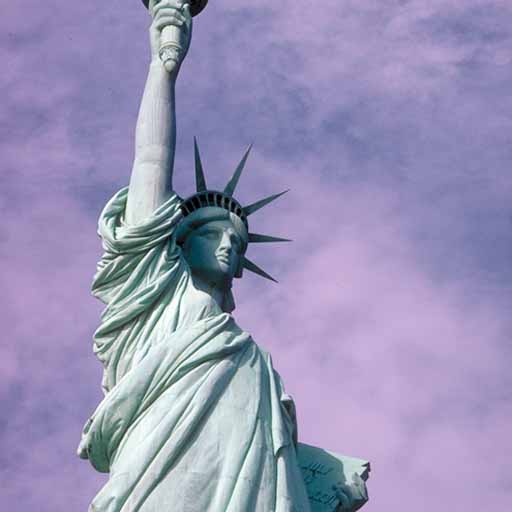
\includegraphics[width=1.4in]{CSIQ/lady_liberty.jpg}
			\centerline{(a)}
		\end{minipage}
		\begin{minipage}[t]{.24\linewidth}
			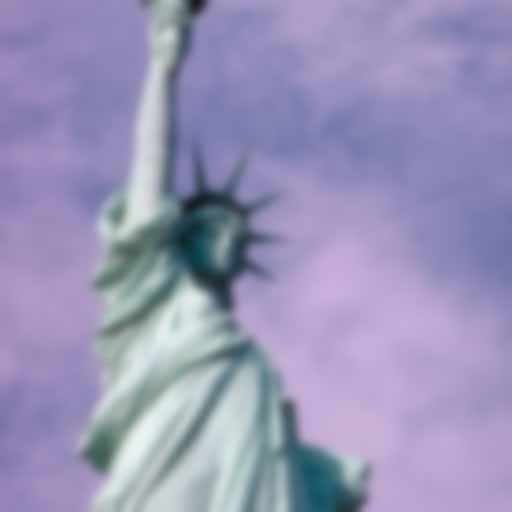
\includegraphics[width=1.4in]{CSIQ/lady_liberty.BLUR.4.jpg}
			\centerline{(b)}
		\end{minipage}
		\begin{minipage}[t]{.24\linewidth}
			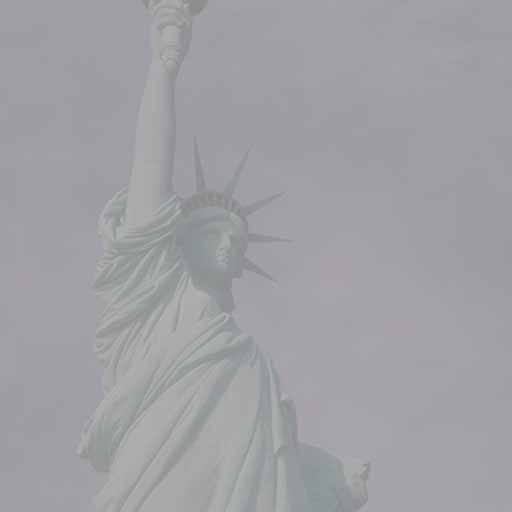
\includegraphics[width=1.4in]{CSIQ/lady_liberty.contrast.3.jpg}
			\centerline{(c)}
		\end{minipage}
		\begin{minipage}[t]{.24\linewidth}
			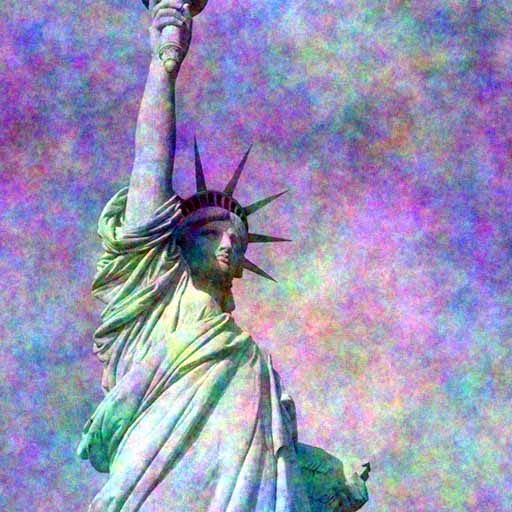
\includegraphics[width=1.4in]{CSIQ/lady_liberty.fnoise.5.jpg}
			\centerline{(d)}
		\end{minipage}
		\begin{minipage}[t]{.24\linewidth}
			\includegraphics[width=1.4in]{CSIQ/monument.jpg}
			\centerline{(e)}
		\end{minipage}
		\begin{minipage}[t]{.24\linewidth}
			\includegraphics[width=1.4in]{CSIQ/monument.BLUR.4.jpg}
			\centerline{(f)}
		\end{minipage}
		\begin{minipage}[t]{.24\linewidth}
			\includegraphics[width=1.4in]{CSIQ/monument.contrast.5.jpg}
			\centerline{(g)}
		\end{minipage}
		\begin{minipage}[t]{.24\linewidth}
			\includegraphics[width=1.4in]{CSIQ/monument.fnoise.5.jpg}
			\centerline{(h)}
		\end{minipage}
		\caption{Demonstrations of the global distortions (b/f: GB, c/g: CC, and d/h: PN) contaminating the Statue of Liberty and George Rogers Clark Memorial images. Figure (a) and Figure (e) are reference images from the CSIQ database.}
		\label{CSIQ-Distortion}
	\end{figure*}
	
	\begin{table*}[!ht]
		\centering
		\caption{The average SRCC and PLCC results of the individual distortion type on the CSIQ database. Top two results are highlighted in bold.}
		\label{individual-CSIQ}
		\resizebox{\linewidth}{!}{
			\begin{tabular}{c|cccccc}
				\toprule
				SRCC & JPEG & JP2K & WN & GB & PN & CC \\ \toprule
				BRISQUE (2012)~\citep{mittal2012no} & 0.806 & 0.840 & 0.723 & 0.820 & 0.378 & 0.804 \\
				CORNIA (2012)~\citep{ye2012unsupervised} & 0.513 & 0.831 & 0.664 & 0.836 & 0.493 & 0.462 \\
				M3 (2014)~\citep{xue2014blind} & 0.740 & 0.911 & 0.741 & 0.868 & 0.663 & 0.770 \\
				HOSA (2016)~\citep{xu2016blind} & 0.733 & 0.818 & 0.604 & 0.841 & 0.500 & 0.716 \\
				FRIQUEE (2017)~\citep{ghadiyaram2017perceptual} & 0.869 & 0.846 & 0.748 & 0.870 & 0.753 & 0.838 \\
				dipIQ (2017)~\citep{ma2017dipiq} & 0.936 & 0.944 & 0.904 & 0.932 & - & - \\
				MEON (2018)~\citep{ma2017end} & \textbf{0.948} & 0.898 & \textbf{0.951} & 0.918 & - & - \\
				WaDIQaM (2018)~\citep{bosse2017deep} & 0.853 & 0.947 & 0.974 & 0.979 & 0.882 & \textbf{0.923} \\
				DB-CNN (2020)~\citep{zhang2018blind} & 0.940 & 0.953 & 0.948 & \textbf{0.947} & \textbf{0.940} & 0.870 \\
				HyperIQA (2020)~\citep{su2020blindly} & 0.934 & \textbf{0.960} & 0.927 & 0.915 & 0.931 & 0.874 \\ \midrule
				\begin{tabular}[c]{@{}c@{}}\textbf{NLNet}\end{tabular} & \textbf{0.972} & \textbf{0.963} & \textbf{0.965} & \textbf{0.955} & \textbf{0.969} & \textbf{0.968} \\ \toprule
				
				PLCC & JPEG & JP2K & WN & GB & PN & CC \\ \midrule
				BRISQUE (2012)~\citep{mittal2012no} & 0.828 & 0.887 & 0.742 & 0.891 & 0.496 & 0.835 \\
				CORNIA (2012)~\citep{ye2012unsupervised} & 0.563 & 0.883 & 0.687 & 0.904 & 0.632 & 0.543 \\
				M3 (2014)~\citep{xue2014blind} & 0.768 & 0.928 & 0.728 & 0.917 & 0.717 & 0.787 \\
				HOSA (2016)~\citep{xu2016blind} & 0.759 & 0.899 & 0.656 & 0.912 & 0.601 & 0.744 \\
				FRIQUEE (2017)~\citep{ghadiyaram2017perceptual} & 0.885 & 0.883 & 0.778 & 0.905 & 0.769 & 0.864 \\
				dipIQ (2017)~\citep{ma2017dipiq} & 0.975 & \textbf{0.959} & 0.927 & 0.958 & - & - \\
				MEON (2018)~\citep{ma2017end} & 0.979 & 0.925 & \textbf{0.958} & 0.946 & - & - \\
				DB-CNN (2020)~\citep{zhang2018blind} & \textbf{0.982} & 0.971 & 0.956 & \textbf{0.969} & \textbf{0.950} & \textbf{0.895} \\ \midrule
				\begin{tabular}[c]{@{}c@{}}\textbf{NLNet}\end{tabular} & \textbf{0.991} & \textbf{0.976} & \textbf{0.967} & \textbf{0.9746} & \textbf{0.966} & \textbf{0.969} \\ \bottomrule
			\end{tabular}
		}
	\end{table*}
	
	\subsubsection{Performance Evaluations of Individual Distortion Type on the TID2013 Database}
	As can be seen from~\reftab{individual-TID2013}, we divide the distortion types into global distortions and local distortions. The local distortions (JPEG transmission errors, JPEG2000 transmission errors, non eccentricity pattern noise, and local block-wise distortions of different intensity) are illustrated in~\reffig{TID2013-Distortion}. Due to the non-local behavior and long-range feature aggregation capability, our method's performance on the globally distorted images is superior to those CNN-based local modeling methods, such as M3~\citep{xue2014blind}, MEON~\citep{ma2017end}, and DB-CNN~\citep{zhang2018blind}. Besides, the NLNet performs well on the noisy images by a large margin, such as those contaminated by the non eccentricity pattern noise ($\uparrow$ 0.346 SRCC), additive noise in color components ($\uparrow$ 0.128  SRCC), comfort noise ($\uparrow$ 0.118 SRCC), additive Gaussian noise ($\uparrow$ 0.084  SRCC), spatially correlated noise ($\uparrow$ 0.032 SRCC), high frequency noise ($\uparrow$ 0.01 SRCC), impulse noise ($\uparrow$ 0.012 SRCC), quantization noise ($\uparrow$ 0.041 SRCC), image denoising ($\uparrow$ 0.017 SRCC), and multiplicative Gaussian noise ($\uparrow$ 0.055 SRCC). This finding is indeed compatible with the results of the Non-local Means denoising, in which the non-local statistics are sensitive to noise. Thus, it successfully assesses noisy images' visual quality with supreme performance. It should also be noted that the non-local nature of spatial filtering preserves the structural information of the image~\citep{buades2011non}. The structural distortion would be sensitively perceptive during the non-local feature aggregation process, leading to an effective and robust IQA method.
	\begin{figure*}[!]
		\centering
		\begin{minipage}[t]{.32\linewidth}
			\includegraphics[width=1.8in]{TID/I15.jpg}
			\centerline{(a)}
		\end{minipage}
		\begin{minipage}[t]{.32\linewidth}
			\includegraphics[width=1.8in]{TID/I12.jpg}
			\centerline{(f)}
		\end{minipage}
		\begin{minipage}[t]{.32\linewidth}
			\includegraphics[width=1.8in]{TID/I05.jpg}
			\centerline{(k)}
		\end{minipage}
		
		\begin{minipage}[t]{.32\linewidth}
			\includegraphics[width=1.8in]{TID/i15_12_4.jpg}
			\centerline{(b)}
		\end{minipage}
		\begin{minipage}[t]{.32\linewidth}
			\includegraphics[width=1.8in]{TID/i12_12_4.jpg}
			\centerline{(g)}
		\end{minipage}
		\begin{minipage}[t]{.32\linewidth}
			\includegraphics[width=1.8in]{TID/i05_12_4.jpg}
			\centerline{(l)}
		\end{minipage}
	
		\begin{minipage}[t]{.32\linewidth}
			\includegraphics[width=1.8in]{TID/i15_13_3.jpg}
			\centerline{(c)}
		\end{minipage}
		\begin{minipage}[t]{.32\linewidth}
			\includegraphics[width=1.8in]{TID/i12_13_5.jpg}
			\centerline{(h)}
		\end{minipage}
		\begin{minipage}[t]{.32\linewidth}
			\includegraphics[width=1.8in]{TID/i05_13_3.jpg}
			\centerline{(m)}
		\end{minipage}
		
		\begin{minipage}[t]{.32\linewidth}
			\includegraphics[width=1.8in]{TID/i15_14_5.jpg}
			\centerline{(d)}
		\end{minipage}
		\begin{minipage}[t]{.32\linewidth}
			\includegraphics[width=1.8in]{TID/i12_14_5.jpg}
			\centerline{(i)}
		\end{minipage}
		\begin{minipage}[t]{.32\linewidth}
			\includegraphics[width=1.8in]{TID/i05_14_5.jpg}
			\centerline{(n)}
		\end{minipage}
	
		\begin{minipage}[t]{.32\linewidth}
			\includegraphics[width=1.8in]{TID/i15_15_1.jpg}
			\centerline{(e)}
		\end{minipage}
		\begin{minipage}[t]{.32\linewidth}
			\includegraphics[width=1.8in]{TID/i12_15_1.jpg}
			\centerline{(j)}
		\end{minipage}
		\begin{minipage}[t]{.32\linewidth}
			\includegraphics[width=1.8in]{TID/i05_15_1.jpg}
			\centerline{(o)}
		\end{minipage}
		
		\caption{Demonstrations of the local distortions (b/g/l: JPEG transmission errors, c/h/m: JPEG2000 transmission errors, d/i/n: non-eccentricity pattern noise, and e/j/o: local block-wise distortions of different intensity). Figure (a), Figure (f), and Figure (k) are reference images from the TID2013 database.}
		\label{TID2013-Distortion}
	\end{figure*}
	\begin{table*}[!ht]
		\centering
		\caption{The average SRCC results of the individual distortion type on the TID2013 database. Top two results are highlighted in bold.}
		\label{individual-TID2013}
		\resizebox{\textwidth}{!}{
			\begin{tabular}{c|c|ccccccc|c}
				\toprule
				SRCC & Distortion Type & BRISQUE~\citep{mittal2012no} & FRIQUEE~\citep{ghadiyaram2017perceptual}& HOSA~\citep{xu2016blind} & MEON~\citep{ma2017end} & M3~\citep{xue2014blind} & DB-CNN~\citep{zhang2018blind} & CORNIA~\citep{ye2012unsupervised} & \begin{tabular}[c]{@{}c@{}}\textbf{NLNet}\end{tabular} \\ \toprule
				
				\multicolumn{1}{c|}{\multirow{20}{*}{\begin{tabular}[c]{@{}c@{}}Global \\Distortion\end{tabular}}} & Additive Gaussian noise & 0.711 & 0.730 & \textbf{0.833} & 0.813 & 0.766 & 0.790 & 0.692 & \textbf{0.917} \\
				\multicolumn{1}{c|}{} & Lossy compression of noisy images & 0.609 & 0.641 & 0.838 & 0.772 & 0.692 & \textbf{0.860} & 0.712 & \textbf{0.935} \\
				\multicolumn{1}{c|}{} & Additive noise in color components & 0.432 & 0.573 & 0.551 & \textbf{0.722} & 0.560 & 0.700 & 0.137 & \textbf{0.850} \\
				\multicolumn{1}{c|}{} & Comfort noise & 0.196 & 0.318 & 0.622 & 0.406 & 0.353 & \textbf{0.752} & 0.617 & \textbf{0.870} \\
				\multicolumn{1}{c|}{} & Contrast change & -0.001 & \textbf{0.585} & 0.362 & 0.252 & 0.155 & 0.548 & 0.254 & \textbf{0.793} \\
				\multicolumn{1}{c|}{} & Change of color saturation & 0.003 & 0.589 & 0.045 & \textbf{0.684} & -0.199 & 0.631 & 0.169 & \textbf{0.827} \\
				\multicolumn{1}{c|}{} & Spatially correlated noise & 0.746 & 0.866 & 0.842 & \textbf{0.926} & 0.782 & 0.826 & 0.741 & \textbf{0.958} \\
				\multicolumn{1}{c|}{} & High frequency noise & 0.842 & 0.847 & 0.897 & \textbf{0.911} & 0.900 & 0.879 & 0.815 & \textbf{0.921} \\
				\multicolumn{1}{c|}{} & Impulse noise & 0.765 & 0.730 & 0.809 & \textbf{0.901} & 0.738 & 0.708 & 0.616 & \textbf{0.913} \\
				\multicolumn{1}{c|}{} & Quantization noise & 0.662 & 0.764 & 0.815 & \textbf{0.888} & 0.832 & 0.825 & 0.661 & \textbf{0.929} \\
				\multicolumn{1}{c|}{} & Gaussian blur & 0.871 & 0.881 & 0.883 & 0.887 & \textbf{0.896} & 0.859 & 0.850 & \textbf{0.912} \\
				\multicolumn{1}{c|}{} & Image denoising & 0.612 & 0.839 & 0.854 & 0.797 & 0.709 & \textbf{0.865} & 0.764 & \textbf{0.882} \\
				\multicolumn{1}{c|}{} & JPEG compression & 0.764 & 0.813 & 0.891 & 0.850 & 0.844 & \textbf{0.894} & 0.797 & \textbf{0.905} \\
				\multicolumn{1}{c|}{} & JPEG 2000 compression & 0.745 & 0.831 & \textbf{0.919} & 0.891 & 0.885 & 0.916 & 0.846 & \textbf{0.930} \\
				\multicolumn{1}{c|}{} & Multiplicative Gaussian noise & 0.717 & 0.704 & 0.768 & \textbf{0.849} & 0.738 & 0.711 & 0.593 & \textbf{0.904} \\
				\multicolumn{1}{c|}{} & Image color quantization with dither & 0.831 & 0.768 & 0.896 & 0.857 & \textbf{0.908} & 0.833 & 0.683 & \textbf{0.911} \\
				\multicolumn{1}{c|}{} & Sparse sampling and reconstruction & 0.807 & 0.891 & \textbf{0.909} & 0.855 & 0.893 & 0.902 & 0.865 & \textbf{0.940} \\
				\multicolumn{1}{c|}{} & Chromatic aberrations & 0.615 & 0.737 & 0.753 & \textbf{0.779} & 0.570 & 0.732 & 0.696 & \textbf{0.773} \\
				\multicolumn{1}{c|}{} & Masked noise & 0.252 & 0.345 & 0.468 & \textbf{0.728} & 0.577 & 0.646 & 0.451 & \textbf{0.700} \\
				\multicolumn{1}{c|}{} & Mean shift (intensity shift) & 0.219 & \textbf{0.254} & 0.211 & 0.177 & 0.119 & -0.009 & 0.232 & \textbf{0.358} \\ \midrule
				
				\multicolumn{1}{c|}{\multirow{4}{*}{\begin{tabular}[c]{@{}c@{}}Local \\Distortion\end{tabular}}} & JPEG transmission errors & 0.301 & 0.498 & 0.730 & 0.746 & 0.375 & \textbf{0.772} & 0.694 & \textbf{0.805} \\
				\multicolumn{1}{c|}{} & JPEG 2000 transmission errors & 0.748 & 0.660 & 0.710 & 0.716 & 0.718 & \textbf{0.773} & 0.686 & \textbf{0.875} \\
				\multicolumn{1}{c|}{} & Non eccentricity pattern noise & 0.269 & 0.076 & 0.242 & 0.116 & 0.173 & \textbf{0.270} & 0.200 & \textbf{0.616} \\
				\multicolumn{1}{c|}{} & Local bock-wise distortions with different intensity & 0.207 & 0.032 & 0.268 & \textbf{0.500} & 0.379 & 0.444 & 0.027 & \textbf{0.493} \\ \bottomrule
			\end{tabular}
		}
	\end{table*}
	
	Furthermore, it obtains state-of-the-art results on the compressed distortions, such as JPEG, JP2K, JPEG transmission errors, JPEG 2000 transmission errors, and lossy compression of noisy images~\footnote{~In some compression systems, the predictive error between the compressed and reference images can be modeled as the double exponential noise, which is a kind of heavy-tailed noises.}. The performance of the individual distortion type has proven that our proposed method is capable of predicting image quality distorted by global distortions with non-local recurrences. It also indicates our model's generalization ability and robustness by integrating the non-local concept into the local modeling method.
	
	\subsubsection{Performance Evaluations of Individual Distortion Type on the KADID-10k Database}
	On the KADID-10k database, the non-eccentricity patch and color block are local distortions (highlighted in blue), and others are globally distributed. Some local distortion examples are shown in~\reffig{KADID-Distortion}. Experimental results of global distortions have verified that the non-local modeling method performs superior to the local modeling-based methods on the globally distributed distortions with non-local recurrences. The reason for this phenomenon is that our method keeps a global modeling capability by learning the non-local features and long-range dependencies.
	\begin{figure*}[!]
		\centering
		\begin{minipage}[t]{.32\linewidth}
			\includegraphics[width=1.8in]{KADID/I38.jpg}
			\centerline{(a)}
		\end{minipage}
		\begin{minipage}[t]{.32\linewidth}
			\includegraphics[width=1.8in]{KADID/I38_20_05.jpg}
			\centerline{(b)}
		\end{minipage}
		\begin{minipage}[t]{.32\linewidth}
			\includegraphics[width=1.8in]{KADID/I38_23_05.jpg}
			\centerline{(c)}
		\end{minipage}
		
		\begin{minipage}[t]{.32\linewidth}
			\includegraphics[width=1.8in]{KADID/I71.jpg}
			\centerline{(d)}
		\end{minipage}
		\begin{minipage}[t]{.32\linewidth}
			\includegraphics[width=1.8in]{KADID/I71_20_05.jpg}
			\centerline{(e)}
		\end{minipage}
		\begin{minipage}[t]{.32\linewidth}
			\includegraphics[width=1.8in]{KADID/I71_23_05.jpg}
			\centerline{(f)}
		\end{minipage}
		
		\begin{minipage}[t]{.32\linewidth}
			\includegraphics[width=1.8in]{KADID/I72.jpg}
			\centerline{(g)}
		\end{minipage}
		\begin{minipage}[t]{.32\linewidth}
			\includegraphics[width=1.8in]{KADID/I72_20_04.jpg}
			\centerline{(h)}
		\end{minipage}
		\begin{minipage}[t]{.32\linewidth}
			\includegraphics[width=1.8in]{KADID/I72_23_05.jpg}
			\centerline{(i)}
		\end{minipage}
		
		\caption{Demonstrations of the local distortions (b/e/h: non-eccentricity patch and c/f/i: color block). Figure (a), Figure (d), and Figure (g) are reference images from the KADID-10k database.}
		\label{KADID-Distortion}
	\end{figure*}
	\begin{table*}[!ht]
		\centering
		\caption{The average SRCC results of the individual distortion type on the KADID-10k database. The local distortions are highlighted in blue and the top two results are highlighted in bold.}
		\label{individual-KADID}
		\resizebox{\textwidth}{!}{
			\begin{tabular}{cc|cccccc|c}
				\toprule
				\multicolumn{2}{c|}{Distortion Type} & BLIINDS-II~\citep{saad2012blind} & BRISQUE~\citep{mittal2012no} & ILNIQE~\citep{zhang2015feature} & CORNIA~\citep{ye2012unsupervised} & HOSA~\citep{xu2016blind} & WaDIQaM~\citep{bosse2017deep} & \begin{tabular}[c]{@{}c@{}}\textbf{NLNet}\end{tabular} \\ \midrule
				\multicolumn{1}{c|}{\multirow{3}{*}{Blurs}} & Lens blur & 0.781 & 0.674 & \textbf{0.846} & 0.811 & 0.715 & 0.730 & \textbf{0.914} \\
				\multicolumn{1}{c|}{} & Gaussian blur & 0.880 & 0.812 & \textbf{0.883} & 0.866 & 0.852 & 0.879 & \textbf{0.914} \\
				\multicolumn{1}{c|}{} & Motion blur & 0.482 & 0.423 & \textbf{0.779} & 0.532 & 0.652 & 0.730 & \textbf{0.899} \\ \midrule
				
				\multicolumn{1}{c|}{\multirow{5}{*}{Color distortions}} & Color diffusion & 0.572 & 0.544 & 0.678 & 0.243 & 0.727 & \textbf{0.833} & \textbf{0.916} \\
				\multicolumn{1}{c|}{} & Color saturation 2 & 0.602 & 0.375 & 0.677 & 0.120 & \textbf{0.841} & 0.836 & \textbf{0.909} \\ 
				\multicolumn{1}{c|}{} & Color quantization & 0.670 & 0.667 & 0.676 & 0.323 & 0.662 & \textbf{0.806} & \textbf{0.853} \\
				\multicolumn{1}{c|}{} & Color shift & -0.139 & -0.182 & 0.090 & -0.002 & 0.050 & \textbf{0.421} & \textbf{0.777} \\
				\multicolumn{1}{c|}{} & Color saturation 1 & 0.091 & 0.071 & 0.027 & -0.019 & \textbf{0.216} & 0.148 & \textbf{0.604} \\ \midrule
				
				\multicolumn{1}{c|}{\multirow{2}{*}{Compression}} & JPEG compression & 0.414 & 0.782 & \textbf{0.804} & 0.556 & 0.582 & 0.530 & \textbf{0.866} \\
				\multicolumn{1}{c|}{} & JPEG 2000 compression & 0.655 & 0.516 & \textbf{0.790} & 0.342 & 0.608 & 0.539 & \textbf{0.853} \\ \midrule
				
				\multicolumn{1}{c|}{\multirow{5}{*}{Noise}} & Denoise & 0.457 & 0.221 & \textbf{0.856} & 0.229 & 0.247 & 0.765 & \textbf{0.953} \\	
				\multicolumn{1}{c|}{} & White noise in color component & 0.757 & 0.718 & 0.841 & 0.418 & 0.745 & \textbf{0.925} & \textbf{0.936} \\			
				\multicolumn{1}{c|}{} & Multiplicative noise & 0.702 & 0.674 & 0.682 & 0.306 & 0.776 & \textbf{0.884} & \textbf{0.934} \\
				\multicolumn{1}{c|}{} & Impulse noise & 0.547 & -0.543 & 0.808 & 0.219 & 0.254 & \textbf{0.814} & \textbf{0.916} \\
				\multicolumn{1}{c|}{} & White Gaussian noise & 0.628 & 0.708 & 0.776 & 0.357 & 0.680 & \textbf{0.897} & \textbf{0.914} \\ \midrule

				\multicolumn{1}{c|}{\multirow{3}{*}{Brightness change}} & Brighten & 0.458 & 0.575 & 0.301 & 0.227 & \textbf{0.753} & 0.685 & \textbf{0.822} \\
				\multicolumn{1}{c|}{} & Darken & 0.439 & 0.405 & 0.436 & 0.206 & \textbf{0.744} & 0.272 & \textbf{0.647} \\
				\multicolumn{1}{c|}{} & Mean Shift & 0.112 & 0.144 & 0.315 & 0.122 & \textbf{0.591} & \textbf{0.348} & 0.335 \\ \midrule
				
				\multicolumn{1}{c|}{\multirow{5}{*}{Spatial distortions}} & Jitter & 0.629 & 0.672 & 0.441 & 0.719 & 0.391 & \textbf{0.778} & \textbf{0.899} \\
				\multicolumn{1}{c|}{} & Pixelate & 0.196 & 0.648 & 0.577 & 0.587 & \textbf{0.702} & 0.700 & \textbf{0.814} \\
				\multicolumn{1}{c|}{} & Quantization & \textbf{0.781} & 0.714 & 0.571 & 0.259 & 0.681 & 0.735 & \textbf{0.791} \\
				\multicolumn{1}{c|}{} & \color{blue}{Color block} & -0.020 & 0.067 & 0.003 & 0.094 & \textbf{0.388} & 0.160 & \textbf{0.440} \\
				\multicolumn{1}{c|}{} & \color{blue}{Non-eccentricity patch} & 0.083 & 0.191 & 0.218 & 0.121 & \textbf{0.461} & 0.348 & \textbf{0.433} \\ \midrule
				
				\multicolumn{1}{c|}{\multirow{2}{*}{Sharpness and contrast}} & High sharpen & -0.015 & 0.361 & \textbf{0.681} & 0.114 & 0.230 & 0.558 & \textbf{0.932} \\
				\multicolumn{1}{c|}{} & Contrast change & 0.062 & 0.105 & 0.072 & 0.125 & \textbf{0.452} & 0.421 & \textbf{0.513} \\ \bottomrule
			\end{tabular}
		}
	\end{table*}
	
	Besides, we discuss the implications of non-local modeling on the individual distortion. In~\reftab{individual-KADID}, the non-local modeling promotes the performance of the noise-related and compression-related distortions, such as impulse noise ($\uparrow$ 0.102 SRCC), denoise ($\uparrow$ 0.097 SRCC), white Gaussian noise ($\uparrow$ 0.017 SRCC), white noise in color component ($\uparrow$ 0.011 SRCC), multiplicative noise ($\uparrow$ 0.05 SRCC), JPEG ($\uparrow$ 0.062 SRCC), and JP2K ($\uparrow$ 0.063 SRCC). In addition, compared with WaDIQaM~\citep{bosse2017deep}, our proposed NLNet performs excellent on distortions of color shift, color saturation 1, JPEG, JP2K, denoise, brighten, darken, color block, and high sharpen. It has shown the advantage of integrating the non-local features with local features for visual quality assessment.
	
	In addition, the NLNet achieves competing performances on the locally distorted images, such as color block-distorted and non-eccentricity patch-distorted images. The reason is that a local modeling method,~\ie, VGGNet-16, is employed in our work. Thus, our proposed method can predict both globally and locally distorted images with competitive performance.
	
	\subsubsection{Four Common Distortion Types on the LIVE, CSIQ, and TID2013 Databases}
	We also provide performance comparisons of four common distortion types,~\ie, WN, GB, JPEG, and JP2K. As shown in~\reftab{common-distortion-types}, the promising performances indicate that our method is robust to assess visual quality distorted by the most widely-used types.
	\begin{table*}[!ht]
		\centering
		\caption{The average SRCC comparisons of four common distortion types on the LIVE, CSIQ, and TID2013 databases. Top two results are highlighted in bold.}
		\label{common-distortion-types}
		\resizebox{\linewidth}{!}{
			\begin{tabular}{c|c|ccccccccccc}
				\toprule
				\multirow{2}{*}{Dataset} & \multirow{2}{*}{Dist.Type} & \multicolumn{11}{c}{Method} \\ \cline{3-13} 
				&  & BRISQUE~\citep{mittal2012no} & BLIINDS-II~\citep{saad2012blind}  & DIIVINE~\citep{moorthy2011blind} & HOSA~\citep{xu2016blind} & CORNIA~\citep{ye2012unsupervised} & WaDIQaM~\citep{bosse2017deep} & DIQA~\citep{kim2018deep} & BPRI (c)~\citep{min2017blind} & BPRI (p)~\citep{min2017blind} & \multicolumn{1}{c|}{TSPR~\citep{min2017blind}} & \begin{tabular}[c]{@{}c@{}}\textbf{NLNet}\end{tabular} \\ \midrule
				\multirow{4}{*}{LIVE} & WN & 0.979 & 0.947 & \textbf{0.988} & 0.975 & 0.976 & 0.970 & \textbf{0.988} & 0.984 & 0.985 & \multicolumn{1}{c|}{0.972} &  \textbf{0.990} \\
				& GB & 0.951 & 0.915 & 0.923 & 0.954 & \textbf{0.969} & 0.960 & 0.962 & 0.927 & 0.924 & \multicolumn{1}{c|}{\textbf{0.978}} & 0.964 \\
				& JPEG & 0.965 & 0.950 & 0.921 & 0.954 & 0.955 & 0.964 & \textbf{0.976} & 0.967 & \textbf{0.967} & \multicolumn{1}{c|}{0.947} & \textbf{0.979} \\
				& JP2K & 0.914 & 0.930 & 0.922 & 0.954 & 0.943 & 0.949 & \textbf{0.961} & 0.908 & 0.907 & \multicolumn{1}{c|}{0.950} & \textbf{0.958} \\ \midrule
				
				\multirow{4}{*}{CSIQ} & WN & 0.682 & 0.760 & 0.866 & 0.604 & 0.664 & 0.929 & 0.835 & 0.931 & \textbf{0.936} & \multicolumn{1}{c|}{0.910} & \textbf{0.965} \\
				& GB & 0.808 & 0.877 & 0.872 & 0.841 & 0.836 & \textbf{0.958} & 0.870 & 0.904 & 0.900 & \multicolumn{1}{c|}{0.908} & \textbf{0.955} \\
				& JPEG & 0.846 & 0.899 & 0.800 & 0.733 & 0.869 & 0.921 & 0.931 & 0.918 & 0.930 & \multicolumn{1}{c|}{\textbf{0.944}} & \textbf{0.972} \\
				& JP2K & 0.817 & 0.867 & 0.831 & 0.818 & 0.846 & 0.886 & \textbf{0.927} & 0.863 & 0.862 & \multicolumn{1}{c|}{0.896} & \textbf{0.963} \\ \midrule
				
				\multirow{4}{*}{TID2013} & WN & 0.858 & 0.647 & 0.855 & 0.817 & 0.817 & 0.843 & 0.915 & \textbf{0.918} & \textbf{0.918} & \multicolumn{1}{c|}{0.876} & \textbf{0.904} \\
				& GB & 0.814 & 0.837 & 0.834 & 0.870 & 0.840 & 0.861 & \textbf{0.912} & \textbf{0.873} & 0.859 & \multicolumn{1}{c|}{0.837} & \textbf{0.912} \\
				& JPEG & 0.845 & 0.836 & 0.628 & \textbf{0.986} & 0.896 & \textbf{0.931} & 0.875 & 0.907 & 0.910 & \multicolumn{1}{c|}{0.913} & 0.905 \\
				& JP2K & 0.893 & 0.888 & 0.853 & 0.902 & 0.901 & \textbf{0.932} & 0.912 & 0.883 & 0.868 & \multicolumn{1}{c|}{\textbf{0.935}} & 0.930 \\ \bottomrule
			\end{tabular}
		}
	\end{table*}

\subsection{Cross-Database Evaluations}
We further analyze the generalization capability of our model in a cross-database manner. As shown in~\reftab{Cross Database Evaluation}, our method achieves the best performances in terms of both SRCC and PLCC on the LIVE (Train) $\rightarrow$ CSIQ (Test), CSIQ (Train) $\rightarrow$ LIVE (Test), and TID2013 (Train) $\rightarrow$ LIVE (Test) settings. As shown in~\reftab{Cross Database Evaluation}, we can observe the setting that training on the CSIQ or LIVE database and testing on the TID2013 database is much more challenging, as many distortion types in the TID2013 database are unseen during training. However, our method still achieves a comparable performance. The superior performance in the cross-database settings reveals the high generalization capability of our method, making our method to be more practical in real applications.
\begin{table*}[!ht]
	\centering
	\caption{Cross-database performance comparisons.}
	\label{Cross Database Evaluation}
%	\resizebox{\linewidth}{!}{
		\begin{tabular}{ccccccc}
			\toprule
			Training & \multicolumn{2}{c}{LIVE} & \multicolumn{2}{c}{CSIQ} & \multicolumn{2}{c}{TID2013} \\ 
			Testing & \multicolumn{1}{c}{CSIQ} & TID2013 & \multicolumn{1}{c}{LIVE} & TID2013 & \multicolumn{1}{c}{LIVE} & CSIQ \\ 
			\midrule
			BRISQUE (2012)~\citep{mittal2012no} & \multicolumn{1}{c}{0.562} & 0.358 & \multicolumn{1}{c}{0.847} & 0.454 & \multicolumn{1}{c}{0.790} & 0.590 \\
			CORNIA (2012)~\citep{ye2012unsupervised} & \multicolumn{1}{c}{0.649} & 0.360 & \multicolumn{1}{c}{0.853} & 0.312 & \multicolumn{1}{c}{0.846} & 0.672 \\
			M3 (2015)~\citep{xue2014blind} & \multicolumn{1}{c}{0.621} & 0.344 & \multicolumn{1}{c}{0.797} & 0.328 & \multicolumn{1}{c}{0.873} & 0.605 \\
			HOSA (2016)~\citep{xu2016blind} & \multicolumn{1}{c}{0.594} & 0.361 & \multicolumn{1}{c}{0.773} & 0.329 & \multicolumn{1}{c}{0.846} & 0.612 \\
			FRIQUEE (2017)~\citep{ghadiyaram2017perceptual} & \multicolumn{1}{c}{0.722} & 0.461 & \multicolumn{1}{c}{0.879} & 0.463 & \multicolumn{1}{c}{0.755} & 0.635 \\
			DIQaM-NR (2018)~\citep{bosse2017deep} & \multicolumn{1}{c}{0.681} & 0.392 & \multicolumn{1}{c}{-} & - & \multicolumn{1}{c}{-} & 0.717 \\
			DB-CNN (2020)~\citep{zhang2018blind} & \multicolumn{1}{c}{\textbf{0.758}} & \textbf{0.524} & \multicolumn{1}{c}{0.877} & \textbf{0.540} & \multicolumn{1}{c}{\textbf{0.891}} & \textbf{0.807} \\ 
			HyperIQA (2020)~\citep{su2020blindly} & \multicolumn{1}{c}{0.697} & \textbf{0.538} & \multicolumn{1}{c}{\textbf{0.905}} & \textbf{0.554} & \multicolumn{1}{c}{0.839} & 0.543 \\ 
			\begin{tabular}[c]{@{}c@{}}\textbf{NLNet}\end{tabular} & \multicolumn{1}{c}{\textbf{0.771}} & 0.497 & \multicolumn{1}{c}{\textbf{0.923}} & 0.516 & \multicolumn{1}{c}{\textbf{0.895}} & \textbf{0.730} \\ \bottomrule
		\end{tabular}
%	}
\end{table*}

\subsection{Ablation Study}\label{Ablation Study}
To verify the functionalities and effectiveness of different components in our model, we conduct an ablation study on the CSIQ database. The experimental results are shown in~\reftab{Ablation Study of different modules}.
\begin{table*}[!ht]
	\centering
	\caption{The results of ablation study.}
	\label{Ablation Study of different modules}
	\begin{tabular}{ccc|cc|cc}
		\toprule
		Non-local block & ${L}_{r}$ & ${L}_{t}$ & PLCC $\uparrow$ & $\Delta$ & SRCC $\uparrow$ & $\Delta$ \\ \hline
		$\checkmark$ & $\checkmark$ & $\checkmark$ & 0.941 & - & 0.958 & - \\ \hline
		& $\checkmark$ & $\checkmark$ & 0.936 & -0.005 & 0.951 & -0.007 \\
		$\checkmark$ &  &  & 0.916 & -0.025 & 0.938 & -0.020 \\
		$\checkmark$ & $\checkmark$ &  & 0.929 & -0.012 & 0.945 & -0.013 \\
		$\checkmark$ &  & $\checkmark$ & 0.934 & -0.007 & 0.947 & -0.011 \\ 
		\bottomrule
	\end{tabular}
\end{table*}
As shown in the table, when we ablate the non-local block from the NLNet, a performance drop can be observed, revealing that the non-local modeling plays an essential and complementary role to the local modeling. In addition, we explore the importance of the quality ranking loss ${L}_{r}$ or the distortion type identification loss ${L}_{t}$. The ablation result shown in~\reftab{Ablation Study of different modules} reveals that the rank learning and distortion type identification contribute to the final performance improvement. We believe the reason may lie in that more discriminative features can be obtained when the quality ranking and distortion identification are performed. Overall, we can conclude that each component of our method provides an influential contribution to the final performance achievement. 
\begin{table*}[!ht]
	\centering
	\caption{Validation performances regarding different hyperparameters in NLNet.}
	\label{Ablation Study of numbers of heads, neurons, and GNN layers}
	\begin{tabular}{cccccc}
		\toprule
		Setting & \begin{tabular}[c]{@{}c@{}}Num. of \\ heads\end{tabular} & \begin{tabular}[c]{@{}c@{}}Num. of\\ neurons\end{tabular} & \begin{tabular}[c]{@{}c@{}}Num. of\\ layers\end{tabular} & SRCC & PLCC \\ \midrule
		1 & \textbf{1} & 32 & 3 & 0.936 & 0.953 \\
		2 & \textbf{4} & 32 & 3 & 0.941 & 0.958 \\
		3 & \textbf{8} & 32 & 3 & 0.938 & 0.949 \\ \midrule
		4 & 4 & \textbf{16} & 3 & 0.933 & 0.953 \\
		5 & 4 & \textbf{32} & 3 & 0.941 & 0.958 \\
		6 & 4 & \textbf{64} & 3 & 0.932 & 0.950 \\ \midrule
		7 & 4 & 32 & \textbf{2} & 0.932 & 0.949 \\
		8 & 4 & 32 & \textbf{3} & 0.941 & 0.958 \\
		9 & 4 & 32 & \textbf{4} & 0.936 & 0.952 \\
		\bottomrule
	\end{tabular}
\end{table*}

Moreover, the multi-head self-attention module is introduced in our method. To verify its effectiveness, we further compare our method with only single-head attention utilized (Num. of heads is 1) in~\reftab{Ablation Study of numbers of heads, neurons, and GNN layers}. Again, the performance drops in terms of both PLCC and SRCC. However, the performance will not be improved when the head number increases which may be led by the over-fitting problem due to more parameters introduced. The best number of heads we finally adopt is 4. Furthermore, as shown in the settings $4\sim6$ and settings $7\sim9$ of~\reftab{Ablation Study of numbers of heads, neurons, and GNN layers}, we also explore the optimal numbers of neurons and GNN layers on the CSIQ database, and the best performance can be achieved when we set the numbers of neurons and GNN layers as 32 and 3, respectively.

\section{Chapter Conclusion}
In this paper, we propose a non-local modeling method for NR-IQA inspired by HVS usually perceives image quality with long-range dependencies. The non-local features and long-range dependencies are learned via a two-stage superpixel-based graph neural network, which plays a complementary role with the local modeling. Experimental results on different IQA datasets demonstrate the effectiveness of the proposed method. Besides, the results of the individual distortion type reveal that the non-local modeling method manages to handle a wide variety of globally and uniformly distributed distortions with non-local recurrences. Meanwhile, it also maintains sensitivity to the local nonuniform-distributed distortions. In addition, it particularly holds a stronger prediction capability to assess the noisy and compressed images quality. Lastly, the superior performance in the cross-dataset setting indicates the high generalization capability of our method, shedding light on the exploration of the generalized NR-IQA models.